% PROJECT: <ETD> Electronic Thesis and Dissertation Initiative
%   TITLE: LaTeX report template for ETDs in LaTeX
%  AUTHOR: Neill Kipp, nkipp@vt.edu
%     URL: http://etd.vt.edu/latex/
% SAVE AS: etd.tex
% REVISED: September 6, 1997
% 
%\documentclass[12pt,dvips]{report}
\documentclass[12pt]{report}
\setlength{\textwidth}{6.5in}
\setlength{\textheight}{8.5in}
\setlength{\evensidemargin}{0in}
\setlength{\oddsidemargin}{0in}
\setlength{\topmargin}{0in}

\setlength{\parindent}{0pt}
\setlength{\parskip}{0.1in}

%\usepackage[left=3cm,top=2cm,right=3cm]{geometry}

 \usepackage[hang,small,bf]{caption}

\usepackage[printonlyused,withpage]{acronym}
\usepackage{colortbl}
\usepackage{times}
\usepackage[siunitx]{circuitikz}
%\usetikzlibrary{trees}
%\usetikzlibrary{shapes,snakes}
\usepackage{verbatim}
\usepackage{amsmath}
\usepackage{amssymb}
\usepackage{setspace}
\usepackage{graphicx}
\usepackage{subfigure}
\usepackage{cancel}
\usepackage[colorlinks=true,linkcolor=blue,citecolor=blue]{hyperref}
\def\chapterautorefname{Chapter}
\def\sectionautorefname{Section}
\def\subsectionautorefname{Section}

\usepackage{algorithm}
\numberwithin{algorithm}{chapter}
\usepackage{algorithmic}

\newcommand{\R}{\mathbb{R}}
\newcommand{\Q}{\mathbb{Q}}
\newcommand{\N}{\mathbb{N}}
\newcommand{\Z}{\mathbb{Z}}

\begin{comment}

:Author: Micah Chambers
\end{comment}

\begin{document}
\thispagestyle{empty}
\pagenumbering{roman}
\begin{center}

% TITLE
{\Large 
Full Brain Blood-Oxygen-Level-Dependent Signal Parameter Estimation Using Particle Filters
}

\vfill

Micah C. Chambers

\vfill

Thesis submitted to the Faculty of the \\
Virginia Polytechnic Institute and State University \\
in partial fulfillment of the requirements for the degree of

\vfill

Master of Science \\
in \\
Electrical Engineering

\vfill

Chris L. Wyatt, Chair \\
William T. Baumann\\
Aloysius. A. Beex \\
Daniel J. Stilwell

\vfill

August 30, 2010\\
Blacksburg, Virginia

\vfill

Keywords: BOLD Response, FMRI, Nonlinear Systems, Particle Filter, Bayesian Statistics, System Identification
\\
Copyright 2010, Micah C. Chambers

\end{center}

\pagebreak

\thispagestyle{empty}
\begin{center}

{\large Full Brain Blood-Oxygen-Level-Dependent Signal Parameter Estimation Using Particle Filters}

\vfill

Micah C. Chambers

\vfill

(ABSTRACT)

\vfill

\end{center}

Traditional methods of analyzing functional Magnetic Resonance 
Images use a linear combination of
just a few static regressors. This work demonstrates an alternative
approach using a physiologically inspired nonlinear model. By using a 
particle filter to optimize the model parameters, the computation time
is kept below a minute per voxel without requiring a linearization 
of the noise in the state
variables. The activation results show regions similar to those found in 
Statistical Parametric Mapping; however, there are some notable regions not 
detected by that technique. Though the parameters selected by the particle filter based approach
are more than sufficient to predict the Blood-Oxygen-Level-Dependent signal
response,
more model constraints are needed to uniquely identify a single set
of parameters. This ill-posed nature explains the large discrepancies
found in other research that attempted to characterize the model parameters.
For this reason the final distribution of parameters is more medically relevant
than a single estimate. Because the output of the particle filter is 
a full posterior probability, the reliance on the mean to estimate 
parameters is unnecessary. This work presents
not just a viable alternative to the traditional method of detecting
activation, but an extensible technique of estimating the joint probability
distribution function of the Blood-Oxygen-Level-Dependent Signal parameters.

\vfill

% GRANT INFORMATION

%That this work received support from the Southeastern Universities
%Research Association (SURA) ``Monticello Library Project'' is purely
%coincidental.

\pagebreak

% Dedication and Acknowledgments are both optional
% \chapter*{Dedication}
\chapter*{Acknowledgments}

This thesis would not have been possible without the guidance, advice and
patience of my advisor, Chris Wyatt. I knew nothing about being a researcher
or about medical imaging when I came to him, and he taught me to read broadly
and to always dig deeper. Thank you Dr. Wyatt.

I would also like to thank William Baumann for his help and inspiration. I
have learned an incredible amount reading papers with you and Dr. Wyatt.

The Neuroscientists at Wake Forest have also been extremely helpful. In 
particular I would like to thank Paul Laurienti for help gathering fMRI
data and using SPM.

To my parents, for all the psychological (and financial) help along the way,
thank you so much. You were always there for me, I couldn't
ask for better parents. Love you guys.

Finally I would like to thank my friends, for the support, for the prayer,
and, yes, for the occasional stress-relieving game of Halo, SOASE, and every
type of SC.  You guys are the best. 

\tableofcontents
\pagebreak

\listoffigures
\pagebreak

\listoftables
\pagebreak

\huge
\bfseries
List of Acronyms
\mdseries
\normalsize
\begin{acronym}[CMRO2]
\acro{BOLD}{Blood-Oxygen-Level-Dependent}
\acro{CBF}{Cerebral Blood Flow}
\acro{CBV}{Cerebral Blood Volume}
\acro{CMRO2}{Cerebral Metabolic Rate of Oxygen}
\acro{DC}{Direct Current}
\acro{dHb}{Deoxygenated Hemoglobin}
\acro{EM}{Expectation-Maximization}
\acro{EPI}{Echo Planar Imaging}
\acro{fMRI}{Functional Magnetic Resonance Imaging}
\acro{FMRIB}{Oxford Centre for Functional MRI of the Brain}
\acro{FSL}{FMRIB Software Library}
\acro{FWHM}{Full-Width Half-Maximum}
\acro{GA}{Genetic Algorithms}
\acro{GLM}{General Linear Model}
\acro{HRF}{Hemodynamic Response Function}
\acro{Hb}{Hemoglobin}
\acro{MAD}{Median Absolute Deviation}
\acro{MI}{Mutual Information}
\acro{MR}{Magnetic Resonance}
\acro{MRI}{Magnetic Resonance Imaging}
\acro{MSE}{Mean Squared Error}
\acro{O2Hb}{Oxygenated Hemoglobin}
\acro{ODE}{Ordinary Differential Equation}
\acro{PDF}{Probability Density Function}
\acro{POSSUM}{Physics-Oriented Simulated Scanner for Understanding MRI}
\acro{RF}{Radio Frequency}
\acro{RMSE}{Root Mean Squared Error}
\acro{RMSR}{Root Mean Squared Residual}
\acro{SA}{Simulated Annealing}
\acro{SNR}{Signal-to-Noise Ratio}
\acro{SPM}{Statistical Parametric Mapping}
\acro{T1}{Longitudinal}
\acro{T2}{Spin-Spin}
\acro{TR}{Repetition Time}
\acro{UKF}{Unscented Kalman Filter}
\end{acronym}
\pagebreak

\pagenumbering{arabic}
\pagestyle{myheadings}
\acresetall
\chapter{Introduction}
Traditional methods of analyzing timeseries images produced by 
Functional Magnetic Resonance 
Imaging (FMRI) perform regression using the linear combination of explanatory variables. 
Though adding nonlinear degrees of freedom naturally mandates more computation,
in this thesis I will discuss a Sequential Monte Carlo method of fitting a nonlinear
model a computation cost that would still allow real time calculations for multiple voxels.
More practically, this method is an alternative
method of detecting neural activity from the traditionally
used Statistical Parametric Mapping (SPM). Though more computationally intense,
this method is capable of modeling nonlinear effects, is conceptually simpler
and provides more detailed output. Additionally,
by using a separate particle filter for each single time series it 
is possible to estimate parameters and make real-time predictions
for small neural regions, a feature which could be useful towards real time FMRI 
\cite{DeCharms2005}. Future works will also benefit from the ability to 
apply conditions to the posterior distribution in post-processing without
recalculating parameters; for instance to impose additional 
physiological
constraints. Modeling the BOLD response as a nonlinear system is the
best way to determine the correlation of stimulus sequence with the BOLD
response; yet in the past doing this on a large scale has been far too
computationally taxing. The solution used here takes approximately 40 seconds
for a single voxel's time series (5 minutes in length, with Core 2 Duo Q6600). 

This thesis is organized as follows. In the introduction I will introduce
FMRI, the method by which neural time changing data is detected. This section
will also describe the basic form of the BOLD model - which drives the 
detectable changes in MR signal. \autoref{sec:Prior Works} will discuss other
methods of analyzing FMRI images as well as other techniques that have
been, or could be applied to the nonlinear regression model described here. 
\autoref{sec:Particle Filter} derives the particle filter using Bayesian 
statistics and discusses some practical elements of implementing the 
particle filter algorithm. \autoref{sec:Methods} then goes into further
detail about the specific particle filter configuration used in this work.
This section also describes the pre-processing pipeline. 
The results are described separately for simulated data
and real FMRI data in \autoref{sec:SimulationResults} and \autoref{sec:RealData},
respectively. Finally in \autoref{sec:Conclusion} there is a discussion of
the usefulness and implications of this technique as well as recommendations
for the direction of future works. 

\section{Historic Context}
For the past twenty years, Functional Magnetic Resonance Imaging (FMRI) 
has been at the forefront of cognitive research. Despite its
limited temporal resolution, FMRI is the standard tool for localizing 
neural activation.  Whereas other methods
of analyzing neural signals can be invasive or difficult to acquire, 
FMRI is quick and cheap, and its analysis straight forward.
By modeling the governing equations behind the neural response that
drives FMRI, it is possible to increase the power of FMRI.
The underlying state equations hold important information
about how individual brain regions react to stimuli. The model parameters
on the other hand, hold important information about the patients individual
physiology including existing and future pathologies. In short,
the long chain of events driving FMRI signals contain information 
beyond correlation with stimuli.

In the past fifteen years, a steady stream of studies have built
on the original Blood Oxygen Level Dependent (BOLD) signal 
derivation first described by \cite{Ogawa}.
The seminal work by \cite{Buxton1998} attempted to explain the
time evolution of the BOLD signal using a windkessel model to
describe the local changes in Deoxygenated Hemoglobin content.
Incremental improvements were made to this model until
\cite{Friston2000} brought all the changes together into a single complete 
set of equations. And while there have been numerous adaptations in the model, 
many of them summarized in \cite{Deneux2006}, even the basic versions
have less bias error than the empirically driven \emph{Canonical Hemodynamic Model}
\cite{Deneux2006,Handwerker2004}.
On the other hand BOLD signal models have numbers
of parameters ranging from seven \cite{Riera2004} to 50 \cite{Behzadi2005} 
for a signal as short as 100 samples long. This number of parameters presents
a significant risk of being under-determined and having high computation cost. 
In this work, only the simplest physiologically inspired model will be
used (with 7 parameters), and steps will be taken to make the most of computation
time.

\section{Overview}
\label{sec:Introduction Overview}
Detecting neural activity using the changes in FMRI images is based on 
the Blood Oxygen Level Dependent (BOLD) signal.
The BOLD signal is caused by minute changes in the ratio of Deoxygenated
Hemoglobin to Oxygenated Hemoglobin in blood vessels throughout the brain \cite{Ogawa}.
Because Deoxygenated Hemoglobin (DHb) is paramagnetic, higher concentrations
attenuate the signal detected during T2-weighted Magnetic Resonance Imaging (MRI)
techniques. The most common FMRI imaging technique, due to its rapid repetition 
time (TR), is Echo Planar Imaging (EPI). When axons becomes active,
a large amount of ions quickly flow out of the cell. In order for this
action potential to occur again (and thus for the neuron to fire again),
an active pumping process must move ions back into the
axon. This process of recharging the axon requires extra energy, which temporarily
increases the metabolic rate of oxygen. On a massive scale (cubic millimeter) 
this activation/recharge process happens continuously. However, when a 
particular region of the brain is significantly active, the action potentials
occur more often, resulting in a local increase of the 
Cerebral Metabolic Rate of Oxygen (CMRO2). Thus, if everything else 
stay the same, blood vessels in an active area will 
tend to have less oxygenated hemoglobin, and more deoxygenated hemoglobin
(due to the increased rate at which oxygen is being consumed).
This would then result in an attenuated FMRI signal. However, to
compensate for activation, muscles that
control blood vessels relax allowing increased blood flow,
which actually overcompensates.
This ultimately results in lower than average concentration of 
deoxyhemoglobin. Thus, the BOLD signal consists of a short initial
dip in the MR signal, followed by a prolonged increase in signal
that slowly settles out. It is the overcompensation that provides
the  primary signal detected with FMRI. This cascade of events
is believed to drive a prolonged increased in local metabolism, 
blood flow, blood volume, and oxygenated hemoglobin. The differences
in onsets and recovery times of these variables are what causes the 
distinguishing characteristics of the BOLD signal. Unfortunately, 
FMRI signal levels are all relative: within a particular
person, scanner and run. 

\section{FMRI}
Magnetic Resonance Imaging, MRI, is a method of building 3D images
non-invasively, based on the difference between nuclear spin
relaxation times in different molecules. First, the subject 
is brought into a large magnetic field which causes nuclear spins
to align. Radio Frequency (RF) signals may
then be used to excite nuclear spin away from the base alignment. 
As the nuclei precess back to the alignment of the magnetic
field, they emit detectable RF signals. Conveniently, the
nuclear spins return their original state at different
rates, called the T1 relaxation time, depending on the atoms excited.
Additionally, the
coherence of the spins also decay differently (and roughly an order of 
magnitude faster
than T1 relaxation) based on the properties of the region.
This gives two primary methods of contrasting substances,
which form the basis of T1 and T2 weighted images. Additionally, 
dephasing occurs at two different rates, the T2 relaxation time,
which is unrecoverable, and T2$^*$ relaxation, which is
much faster, but possible to recover from via special RF signals.
T1 relaxation times are typically on the order of seconds if 
a sufficiently strong excitation was applied, whereas T2 relaxation
times are usually less than 100ms. 
In order to rapidly acquire entire brain images, as done in Functional 
MRI, a single large excitation pulse is applied to the entire brain,
and the entire volume is acquired in a single T1 relaxation period. 
Because the entire k-space (spatial-frequency) volume is acquired 
from a single excitation, the signal-to-noise-ratio is low
in EPI. 

Increasing the spatial resolution of EPI necessarily 
requires more time or faster magnetic field switching. Increasing
magnet switching rates can result in
more artifacts and lower signal to noise ratios. The result is
that at best FMRI is capable of 1 second temporal resolution. 
The signal is also diluted because each voxel contains
a variety of neurons, capillaries and veins. 
Thus, the FMRI signal, which is sensitive to the chemical composition of 
materials, is the average signal from various types of tissue
in addition to the blood. As mentioned in \autoref{sec:Introduction Overview},
and explored in depth in \autoref{sec:BOLD Physiology},
the usefulness of FMRI comes from discerning of changes in 
Deoxyhemoglobin/Oxyhemoglobin. Therefore, it is necessary to assume
that the only chemical changes will be in
capillary beds feeding neurons. In practice this may not be the case, for
instance near large veins, and it may explain some of the
noise seen in FMRI imaging (see \autoref{sec:Introduction Noise}. 
Because MRI is unitless and certain
areas will have a higher base MR signal, all FMRI studies deal with
percent change from the base signal; rather than raw values. 

\section{BOLD Physiology}
\label{sec:BOLD Physiology}
It is well known that the two types of hemoglobin act as a contrast agents in 
EPI imaging
\cite{Buxton1998, WEISSKOFF1994, Ogawa}, however the connection
between Deoxyhemoglobin/Oxygenated Hemoglobin and neural activity is non-trivial. 
Intuitively, increased 
metabolism will increase Deoxyhemoglobin, however blood vessels are quick
to compensate by increasing local blood flow. Increased inflow, accomplished by loosening 
capillary beds, precedes increased outflow, driving increased 
blood storage.
Since the local MR signal depends on the ratio of Deoxyhemoglobin to Oxygenated
Hemoglobin, increased blood volume affects this ratio if 
metabolism doesn't exactly match the increased inflow of oxygenated blood.
This was the impetus
for the ground breaking balloon model \cite{Buxton1998} and windkessel
model \cite{Mandeville1999}. These works derive, from first principals,
the changes in deoxyhemoglobin ratio and volume of capillaries given flow waveform.
These were the first two attempts to quantitatively account for the shape of the 
BOLD signal as a consequence of the lag between the cerebral blood volume (CBV) 
and the inward cerebral blood flow (CBF). 

Although \cite{Buxton1998} demonstrated that a well chosen flow waveform could 
explain most features of the BOLD signal, it stopped short of proposing a
realistic waveform for the CBF and CMRO2. In \cite{Friston2000} Friston et. al.
gave a reasonable and simple
expression for CBF input based on a flow inducing signal.
Additionally, in the same work Friston et. al. proposed a simple method
of estimating metabolic rate: as a direct function of the inward blood flow.
By combining these equations with the balloon model from \cite{Buxton1998},
it is possible to predict the BOLD signal directly from a stimulus time course.
\begin{eqnarray}
\dot{s} &=& \epsilon u(t) - \frac{s}{\tau_s} - \frac{f - 1}{\tau_f} \\
\dot{f} &=& s\\
\dot{v} &=& \frac{1}{\tau_0}(f - v^\alpha)\\
\dot{q} &=& \frac{1}{\tau_0}(\frac{f(1-(1-E_0)^f)}{E_0} - \frac{q}{v^{1-1/\alpha}})
\label{eq:bold}
\end{eqnarray}
where $s$ is a flow inducing signal, $f$ is the input blood flow (CBF),
$v$ is normalized cerebral blood volume (CBV), and $q$ is the normalized
local deoxyhemoglobin. The 
parameters controlling blood flow are $\epsilon$, which is a neuronal 
efficiency term, $u(t)$, which is the stimulus, and $\tau_f$, $\tau_s$ 
which are time constants. The parameters for the evolution of blood 
volume are $E_0$ which the resting metabolic
rate and $\alpha$ which is Grubb's parameter controlling the balloon model. 
$\tau_0$ is a single time constant controlling the speed of $v$ and $q$.

This completed balloon model was well summarized again
in \cite{Riera2003}. Ogawa et. al. \cite{Obata2004} refined the readout equation 
of the BOLD signal based on the
deoxyhemoglobin content (q) and local blood volume (v), resulting in the
final BOLD equation:
\begin{eqnarray}
y   &=& V_0((k_1 + k_2)(1-q) - (k_2 + k_3)(1-v))\\
k_1 &=& 4.3 \times \nu_0 \times E_0 \times TE = 2.8\\
K_2 &=& \epsilon_0 \times r_0 \times E_0 \times TE = .57\\
k_3 &=& \epsilon_0 - 1 = .43
\label{eq:boldout}
\end{eqnarray}
Where $\nu_0 = 40.3 s^{-1}$  is the frequency offset in Hz for fully
de-oxygenated blood (at 1.5T), $r_0 = 25 s^{-1}$  is the slope relating
change in relaxation rate with change in blood oxygenation, and
$\epsilon_0 = 1.43$ is the 
ratio of signal MR from intravascular to extravascular regions at rest. Although,
these constants change with experiment ($TE$, $\nu_0$, $r_0$),
patient, and brain 
region ($E_0$, $r_0$), often the estimated values taken from \cite{Obata2004} are 
taken as the constants $a_1 = k_1 + k_2 = 3.4$, and $a_2 = k_2+k_3 = 1$ in 
studies using 1.5 Tesla scanners.
While this model is more accurate than the static Hemodynamic Model used in SPM,
there are other additions which give it more degrees of freedom. 

\section{Post Stimulus Undershoot}
\label{sec:Post Stimulus Undershoot}
Although the most widely used, the BOLD model described in \autoref{eq:bold}
and \autoref{eq:boldout} has been extended in various fashions. The most
significant feature missing from the original model is the 
post-stimulus undershoot.
The post-stimulus undershoot is the term used for a prolonged subnormal
BOLD response for a period of 10 to 60 seconds after stimulus has
ceased \cite{Chen2009,Mandeville1999a}.

Because \autoref{eq:bold} is not capable of producing such a prolonged undershoot,
additional factors must be at play. Two prominent theories exist to explain the post 
stimulus undershoot.  Recall
that a lower than base signal means that there is an increased deoxyhemoglobin
content in the voxel. The first and simplest explanation is that the post-stimulus
undershoot is caused by a prolonged increase in CMRO2 after CBV and CBF
have returned to their base levels. This theory is justified by 
studies that show CBV and CBF returning to the baseline before the BOLD signal
\cite{Frahm2008, Donahue2009, Buxton2004, Lu2004, Shen2008}. 
Unfortunately, because of limitations on FMRI and in vivo
CBV/CBF measurement techniques it is difficult to isolate whether CBF and
CBV truly have returned to their baseline. Other studies indicate
that there can be a prolonged supernormal CBV \cite{Mandeville1999a,
Behzadi2005, Chen2009a}, although none of these papers completely
rule out the possibility of increased CMRO2. The discrepancies may in part
be explained by a spatial dependence in the post-stimulus undershoot; described
by \cite{Yacoub2006}. In \cite{Chen2009}
a compelling case is made that most of the post stimulus undershoot can be 
explained by combination of a prolonged CBV increase, and a prolonged CBF 
undershoot, and that
the previous measurements showing a quick recovery of CBV 
were in fact showing a return to baseline by arterial CBV (which
has little effect on the BOLD signal).

Regardless of the probability that CMRO2 and CBF are detached,
research into the post-stimulus undershoot has led to the creation
of much more in depth models. In \cite{Zheng2002} additional state
variables model oxygen transport, whereas \cite{Buxton2004} models
CMR02 from a higher level, and somewhat more simply; though it 
still adds 9 new parameters. \cite{Behzadi2005}
introduces nonlinearities into the CBF equations as a method to
explain the post-stimulus undershoot, which falls in line with a 
prolonged increase in CBF observed in \cite{Chen2009}. Similarly
\cite{Zheng2005} adds additional compartments to model 
venous and arterial blood. 
In \cite{Deneux2006} Deneux et. al. compared these models and though 
that work did not deal extensively with the 
post-stimulus undershoot, it did show incremental improvements
in quality from the additional parameters. 
Importantly, \cite{Deneux2006} did show that by 
simply adding viscoelastic terms from \cite{Buxton2004}, a slowed return 
to baseline is possible to model, without greatly increasing
complexity. Regardless, because these models are more 
complex, and the parameters are not well characterized, in this work the simple
Balloon model is used. 

In summary, there have been extensive refinements to the Balloon
model; however, the increased complexity and lack of known priors 
make these models difficult to work with. Additional degrees of freedom 
could also make parameter estimation intractable.

\section{Properties of the BOLD Model}
\label{sec:BOLD Analysis}
Since the first complete BOLD model was proposed by \cite{Friston2002}, 
several studies have analyzed its properties. 
The most important property is that the system is dissipative, and given
enough time will converge to a constant value. This is found simply by
analyzing the eigenvalues of the state equation Jacobian, 
\cite{Deneux2006, Hu2009}. The steady state of the Balloon
model equations gives:

\begin{eqnarray}
s_{ss} &=& 0 \nonumber \\
f_{ss} &=& \tau_f\epsilon u + 1\nonumber \\
v_{ss} &=& (\tau_f\epsilon u + 1)^\alpha\nonumber \\
q_{ss} &=& \frac{(\tau_f\epsilon u + 1)^\alpha}{E_0}(1-(1-E_0)^{1/(\tau_f\epsilon u + 1)})\nonumber \\
y_{ss} &=& V_0((k_1+k_2)(1-q_{ss}) - (k_2+k_3)(1-v_{ss}))
\label{eq:steadystate}
\end{eqnarray}

where the parameters are all the same as in \autoref{eq:bold}

In real FMRI data, there is a significant nonlinearity in response; with short sequences
responding disproportionately strongly \cite{Birn2001, Wager2005, Deneux2006}.
This nonlinearity is accounted for in the Balloon model, although \cite{Deneux2006}
shows that when duration of stimuli varies greatly,
modeling Neural Habituation is necessary to fully capture the range of responses. 
In both \cite{Birn2001} and \cite{Deneux2006} it was found that 
stimuli lasting longer than 4 seconds 
tend to be more linear, which is why block designs are so well accounted for
by the General Linear Model (see \autoref{sec:Current Techniques General Linear Model}).

Another interesting result of \cite{Deneux2006} was the sensitivity analysis.
There it was found that the parameters are far from perpendicular,
and that very different parameters could give nearly identical BOLD output.
The means that that without constraining parameter values, they may not be 
precisely ascertainable. This could explain discrepancies in previous studies
(\autoref{tab:Params}).

%note to self, friston2002b's parameters are from a picture
\begin{table}[t]
\centering
\begin{tabular}{|c || c | c | c | c|}
\hline 
Parameter  & \cite{Friston2000} & \cite{Johnston2008} & \cite{Vakorin2007} & \cite{Deneux2006}\\
\hline
$\tau_0  $ &  $N(.98 , .25^2)$  & $8.38 \pm 1.5  $ & $.94$ & .27\\
$\alpha  $ &  $N(.33 , .45^2)$  & $.189 \pm .004 $ & $.4$ (NC) & .63 \\
$E_0     $ &  $N(.34 , .1 ^2)$  & $.635 \pm .072 $ & $.6$ (NC) & .33\\
$V_0     $ &  $.03$ (NC)        & $.0149 \pm .006$ & (NC) & .16\\
$\tau_s  $ &  $N(1.54, .25^2)$  & $4.98 \pm 1.07 $ & $2.2$ & 2.04 \\
$\tau_f  $ &  $N(2.46, .25^2)$  & $8.31 \pm 1.51 $ & $.45$ & 5.26\\
$\epsilon$ &  $N(.54 , .1 ^2)$  & $.069 \pm .014 $ & (NC) & .89\\
\hline
\end{tabular}
\caption{Parameters found by various studies. (NC) indicates that the value
wasn't calculated. \cite{Vakorin2007} made use of the values from \cite{Friston2002}
where not explicitly stated}
\label{tab:Params} 
\end{table}


\chapter{Alternate Methods}
\label{sec:Prior Works}
Currently, \ac{fMRI} is used to determine the location of responses
to stimuli. The method of finding activation is discussed in 
\autoref{sec:Statistical Parametric Mapping}. The goal of this 
work is to move away from simple localization, and move toward
characterizing the response curve. Doing so 
necessitates more complex models and requires
more computation. Already there have been several other
attempts to model the \ac{BOLD} response; these works will be discussed
in this chapter.

\section{Statistical Parametric Mapping}
\label{sec:Statistical Parametric Mapping}
Although not strictly the same as parameter calculation from 
\ac{fMRI}, activation detection is similar and worth discussing. Estimation of 
parameters is a generalization of the idea 
of activation detection.
Given the popularity of \ac{SPM}
it is important to draw a distinction between it and the methods proposed
in this work.

\subsection{Random Field Theory}
\label{sec:RFT}
\ac{SPM} methods make significant use of $t$-Tests across large regions;
however, such $t$-tests work slightly differently than a single
individual test. A $t$-test with a p-value of $0.05$ over 
10,000 voxels, will on average generate 500 false
positives. This is called the multiple comparison problem. Traditional
Bonferroni Correction
deals with this by requiring each test to pass with P
value of $\frac{0.05}{10000}$. The probability of 
a single false positive would then be $0.05$. Unfortunately this leads to unrealistically
low p-values; so low that it would be impossible for any biological system to satisfy. To
compensate, a Gaussian kernel is applied to smooth the image. This has
the benefit of reducing the noise variance and 
decreasing the effective number of independent measurements. Because
the number of \emph{independent} measurements is smaller, Bonferroni correction
can theoretically be applied with a lower scaling factor than
the original voxel count \cite{Worsley2004}. As a side effect of this 
extreme smoothing, a single active voxel is very difficult to detect.

\subsection{Classical Activation Detection}
\label{sec:Square Wave}
The most basic method of analyzing \ac{fMRI} data is by standard $t$-test
between resting state and active state samples. Simply put, the
mean is calculated separately for non-stimulus and stimulus time intervals.
A classic $t$-test may then be applied, giving the probability that the
distributions actually have the same mean. Because of the correlated
noise present in \ac{fMRI} (\autoref{sec:Introduction Noise}), it is necessary
to apply a high-pass filter to the data. Without applying
such a filter, T-values must be set extraordinarily high to prevent
false positives \cite{Smith2007}. Because the \ac{BOLD} response is known
not to fit a square wave this method is rarely used
(\autoref{sec:BOLD Physiology}). For this reason other methods
are often more used, as discussed in 
\autoref{sec:Current Techniques General Linear Model}.

\subsection{General Linear Model}
\label{sec:Current Techniques General Linear Model}
The most common \ac{fMRI} analysis tool is \ac{SPM}, which generates
statistical parametric map using more advanced methods than a simple
square wave. Hierarchal
Models are one important improvement that allows researchers
to combine data across multiple runs, patients and stimuli
(see \cite{Hofmann1997} for more on Hierarchical Modeling). 
Hierarchical Models
concatenate all the data into a single dataset, then perform
a linear fit between a design matrix and the data. The design matrix
encapsulates all known experimental factors such as stimuli,
young/old, etc.  The general linear model is defined as:

\begin{equation}
Y(t) = X(t)\beta + \epsilon(t)
\end{equation}

where $Y(t)$ is the smoothed or de-trended time course of measurements,
$X(t)$ is the design matrix, $\beta$ is a column vector of weights,
and $\epsilon$ is the error. Thus for every time, the measurement is
assumed to be a weighted sum of the columns of $X$ plus some error. The calculation
of $\beta$ is then performed using a maximum likelihood or gradient descent search 
to minimize the error. 

\begin{figure}
\centering
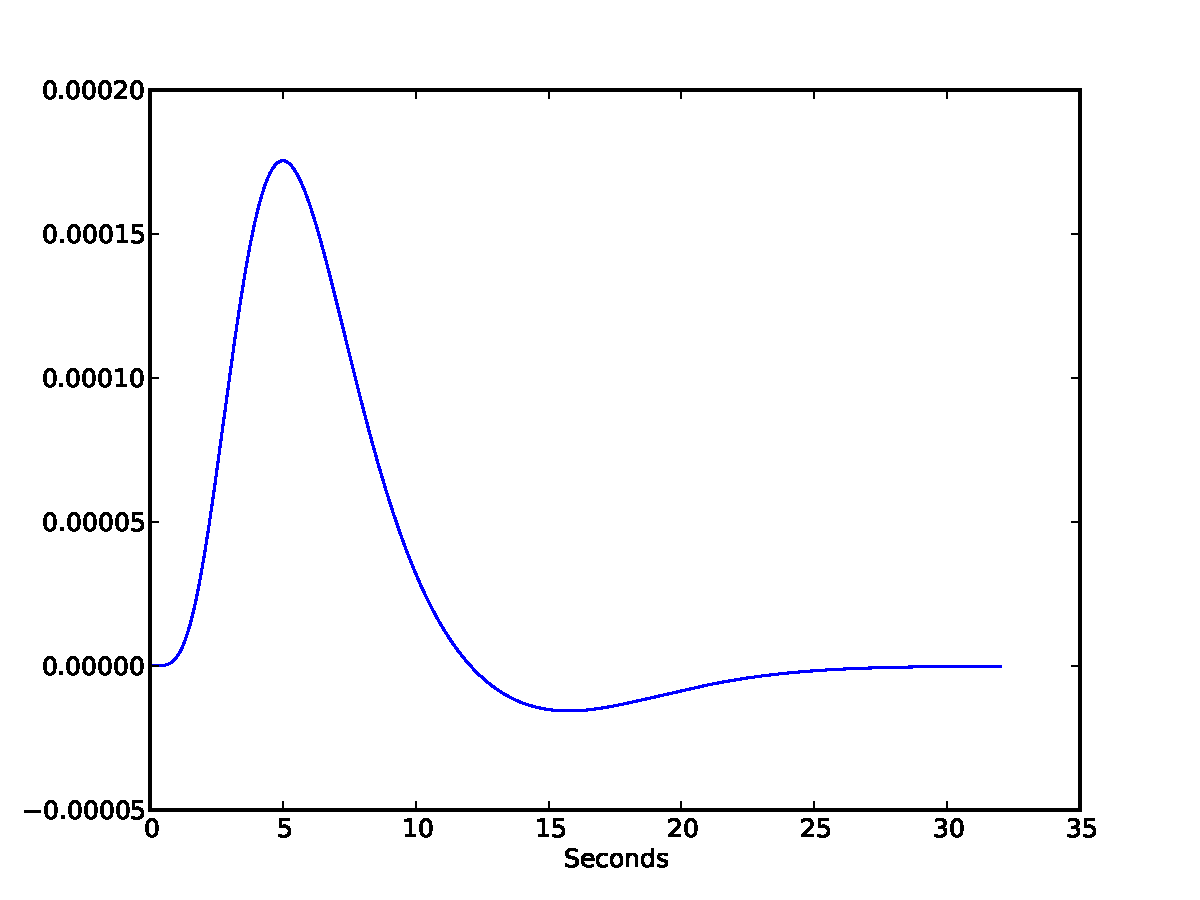
\includegraphics[scale=.7]{images/HRF}
\caption{Canonical Hemodynamic Response Function (y-axis units are arbitrary because 
normalization is performed).}
\label{fig:HRF}
\end{figure}

As mentioned previously, a square wave stimulus 
does not result in a square wave in the activation of brain regions. 
The \ac{BOLD} signal is in fact a smoothed version of the 
stimuli. As such, when fitting an \ac{fMRI} time course to the input,
the input ($X$'s columns) is usually smoothed to reduce bias error. 
The best method, that maintains a linear fit, is convolving the input 
with a \ac{HRF}. The \ac{HRF}
mimics the basic shape of \ac{BOLD} activation, including a delay
due to rise time and fall time. The fitting 
process is then a least squares fit over the space of the vector $\beta$. 
Therefore $Y(t)$ is estimated as a linear combination 
of the columns of $X$. 

Smoothing the input with a single \ac{HRF} poses certain problems.
It is well known that different Hemodynamic Response Functions are necessary 
for different regions of the brain \cite{Handwerker2004}. The Canonical 
\ac{HRF} that is most often used, 
has been optimized for the visual cortex. As discussed in \autoref{sec:Post Stimulus Undershoot},
there are definitely variations in the shape of the
\ac{BOLD} response, over both brain regions and patients. Handwerker et. al. 
discussed the implications of choosing an incorrect \ac{HRF}, the most important
of which is a definite increase in false negatives \cite{Handwerker2004}. While an atlas
of Hemodynamic Response Functions for each region could definitely 
mitigate this risk, it does not account for variation between patients.

\subsection{Hierarchical Linear Models}
As mentioned previously and discussed extensively
in Friston et al. \cite{Friston2002a} and Hoffman et al. \cite{Friston2002a},
hierarchical models may be 
applied to account for systematic differences between subjects.
For instance, if the
study mixes young and old subjects, incorporating
that into the model is wise, regardless of whether it is the goal of the test. 
The reason to do this is to account for additional variance that may not
be otherwise explainable.  The Hierarchical form used by
Friston et al. \cite{Friston2002a} the \ac{GLM} which 
is shown in \autoref{eq:Hierarchical} .

\begin{eqnarray}
\label{eq:Hierarchical}
Y(t) & = & X_1(t)\theta_1 + \epsilon_1(t)            \nonumber \\
\theta_1(t) &=& X_2(t)\theta_2 + \epsilon_2(t)     \nonumber \\
 & ... &                                             \nonumber \\
\theta_{n-1}(t)& =& X_n(t)\theta_n + \epsilon_n(t) 
\end{eqnarray}

The Empirical Bayes algorithm was used by both Friston et al. \cite{Friston2002a}
and Hofmann et al. \cite{Hofmann1997}. Note that in Empirical Bayes, 
point estimators are used for each $\theta$, rather than full 
distributions or the first two moments.

\subsection{Discussion}
\label{sec:BackgroundConclusion}
In all, the \ac{GLM} is useful for determining linear 
dependence of a set of regressors on the output. Unfortunately, as discussed in
\autoref{sec:BOLD Analysis} there are significant nonlinearities 
that almost certainly cause false negatives in the Statistical Parametric
Maps. Unfortunately nonlinear analyses have only recently become feasible,
so the scale of the problem is still unknown. The problem is 
highlighted by the common scenario where no significant
activation can be found in a single run \cite{Riera2003, Johnston2007}.  

The static nature of the  linear model also limits its potential use. 
Besides not allowing \ac{HRF} differences between patients, there is no
reasonable way to incorporate other forms of physiological
data. Combined \ac{fMRI} \ac{CBF} or \ac{CBV} imaging methods are improving,
as seen in Chen et al. \cite{Chen2009}. These techniques could shed light on
neural activation by providing extra measurements, yet a 
physiologically reasonable model is necessary to incorporate this extra data.
Activation detection methods also don't have the ability 
to identify pathologies based on state variables or parameters. For
example, decreased compliance of
blood vessels could indicate, or even cause, a neurological condition that 
is not easily seen in other imaging modalities. 

\section{Approaches to the Balloon Model}
Unlike Statistical Parametric Mapping, the techniques described in this
section are all attempts to regress some version of the \ac{BOLD} model. 
Although Buxton et al. \cite{Buxton1998} and Friston et al. \cite{Friston2000}
both proposed physiologically reasonable values for the model parameters, 
Friston et al. \cite{Friston2002b} was the first paper to calculate the 
parameters based on actual \ac{fMRI} data. 
However, in that case, the voxels were chosen from
regions that were detected as active by the \ac{GLM}. It is therefore possible
that the parameters are biased toward parameters that fit the linear model.

\subsection{Polynomial Approximation}
\label{sec:Background Linear Approximation}
In Friston et al. \cite{Friston2002b}, a novel combination of 
linear and nonlinear modeling proposed to generate parameter estimates. 
Because there is no closed 
form solution to the balloon model, it is impossible to 
calculate the Jacobian matrix $\frac{\partial Y}{\partial \theta}$. Thus 
Friston et al. \cite{Friston2002b} approximated the partial using a
low-order Volterra Kernel. 
At each step of the \ac{EM} algorithm, 
the differential equation was integrated and the residuals
calculated. Then, for each $\theta_i$ surrounding the estimate of 
$\theta$, a Volterra Kernel expansion of the output $y$ was generated. Generation
of the Volterra Kernel is quick, and, since there
is an analytical solution, calculating partial derivatives is easy. 
Unfortunately, it was found in that work that estimating a Volterra kernel
took longer than simply integrating the state variables. 
The full E-M algorithm for estimating the states is notation-heavy 
 and can be found in Friston et al. \cite{Friston2002b}.

There are a few caveats with this method of optimization. First, the 
partials are based on approximate values (using Volterra-Kernels) of $y$.
Importantly, the Volterra-Expansion of $y$ is not able to model interactions
between state variables; which certainly increases error \cite{Friston2002b}.
Additionally, to date no extensive review of the accuracy of the 
Volterra expansion has been performed. Finally all the tests performed
by Friston et al. were on regions found to be active by the General
Linear Model \cite{Friston2002b}. For this reason, the reliability of 
the approximation is unknown for regions that are active but sufficiently 
nonlinear to avoid detection by conventional tests.

\subsection{Nonlinear Least Squares}
\label{sec:Nonlinear Least Squares}
Although there are certainly benefits to using a derived model, rather
than a purely empirical model, there are serious implications. The
first problem is that all the powerful linear techniques of gradient
descent are off limits; since the model is a true nonlinear dynamical
system with no closed form solution (although \autoref{sec:Background Linear Approximation}
circumvented this by calculating a Volterra Series approximation). Without
a Jacobian for residuals, the Gauss-Newton method
is impossible. Additionally, a gradient descent is slow
without the ability to form partials of the output with respect
to all the parameters. 

Still, there are other heuristic algorithms
that could estimate the \ac{BOLD} response. 
\ac{SA} is a common method of optimizing high dimensional
regression problems. First the program selects a random starting point, then
at each iteration it selects a random point in the neighborhood. If the 
new point is 
below some energy constraint (energy is a function of the residual), 
called the temperature, the algorithm moves
to that point and continues with the next iteration. The temperature
is slowly lowered until no nearby points below the temperature can
be found. There are
variations of this, for instance it is common to require every movement
to be in the downward direction (in terms of energy). Like most nonlinear
optimization problems, there is no guarantee of an optimal solution,
although the longer the algorithm is allowed to run, the better the solution.
Since every step requires a re-integration of the  
balloon model, it can be extremely time consuming, which is why I did 
not use it here.

%\begin{algorithm}
%\caption{Simulated Annealing Algorithm}
%\label{alg:Simulated Annealing}
%\begin{algorithmic}
%\STATE Initialize $\Theta$, or if there exists a decent estimate start there
%\STATE Initialize temperature, T to value above initial energy
%\WHILE{$E(\Theta) < T$}
%    \REPEAT
%        \STATE Pick $\theta$ near $\Theta$
%        \STATE Calculate energy, $E$, of $\theta$
%    \UNTIL{$E > T$}
%    \STATE Move to new estimate: set $\Theta = \theta$
%\ENDWHILE
%\end{algorithmic}
%\end{algorithm}

\ac{GA} are similar to Simulated Annealing, in
that they randomly move to better solutions based on a cost function.
However, in genetic algorithms, a single point estimate isn't used. Instead
a population of estimates is generated, each with distinct parameters,
and then each set of parameters is rated with a fitness function. Parameter
sets that are good get a higher weight. New parameter sets are generated by 
randomly combining pieces of the old parameter sets. The pieces are 
chosen at a rate proportional to the fitness of the donor; thus good
parameter sets tend to pass on their properties. In addition to this,
random mutations are introduced that come from no existing parent. 
The fitness function is then used to weight the new generation, and
the entire process starts over. The stop condition for a genetic algorithm
is typically based on some threshold for fitness or a maximum number 
of generations. As with simulated annealing (or any generic non-linear optimization),
there is no guarantee that a global minimum has been reached.

%\begin{algorithm}
%\caption{Genetic Algorithm}
%\label{alg:Genetic Algorithm}
%\begin{algorithmic}
%\STATE Initialize $N$ estimates, $E = \{\Theta_0, \Theta_1, ... \Theta_N\}$
%\FOR{G generations}
%    \STATE Calculate fitness for each $\Theta$, Ex. for residual $R$, $1/R$ or, $e^{-R}$
%    \FOR{$i$ in $N$}
%        \STATE Randomly select two parents (with higher probability for more fit $\Theta$'s)
%        \STATE Randomly merge parts of the two parents to form a new $\Theta_i$
%        \STATE With low probability introduce random mutations to parameters in $\Theta_i$
%    \ENDFOR
%\ENDFOR
%\end{algorithmic}
%\end{algorithm}

Although both these methods can be highly effective, they have the downside of
requiring high computation time. In the case of the \ac{BOLD} model,
each time the energy or fitness needs to be calculated, a large number of cycles
must be spent re-simulating the \ac{BOLD} model for the set of parameters. As I'll
discuss in \autoref{sec:Particle Filter}, the Particle Filter method is able
to circumvent this re-calculation to some degree. Its worth noting though, that 
to beat the particle filter algorithm discussed in \autoref{sec:Particle Filter} 
these would have to converge in less than 1000 simulations (which is far less than
1000 generations in \ac{GA}). 

\subsection{Unscented Kalman Filter}
\label{sec:Unscented Kalman Filter}
The \ac{UKF} is a powerful Gaussian/Bayes filter that attempts
to model the posterior distribution of dynamical systems as a multivariate
Gaussian. The \ac{UKF} generalizes the Extended Kalman
Filter by allowing the state update and output functions to be arbitrary functions.

\begin{eqnarray}
X(t) &=& g(u(t), X(t-1))\\
Y(t) &=& h(X(t))
\end{eqnarray}

In order to estimate the posterior at $t$, a deterministic set of sigma points 
(often 2 per dimension, plus 1 at the mode of the multivariate distribution)
weighted according to a Gaussian estimate of $X(t-1)$ are passed through
the update equation. This set of points are then used to estimate the 
mean and covariance of $X(t)$. The benefit of this is that it requires
no Jacobian and only a few extra calculations to get a decent estimate of
a posterior Gaussian. Hu et. al. used the \ac{UKF} to  perform a similar type of analysis to
the one performed in this work \cite{Hu2009}. 

\begin{figure}
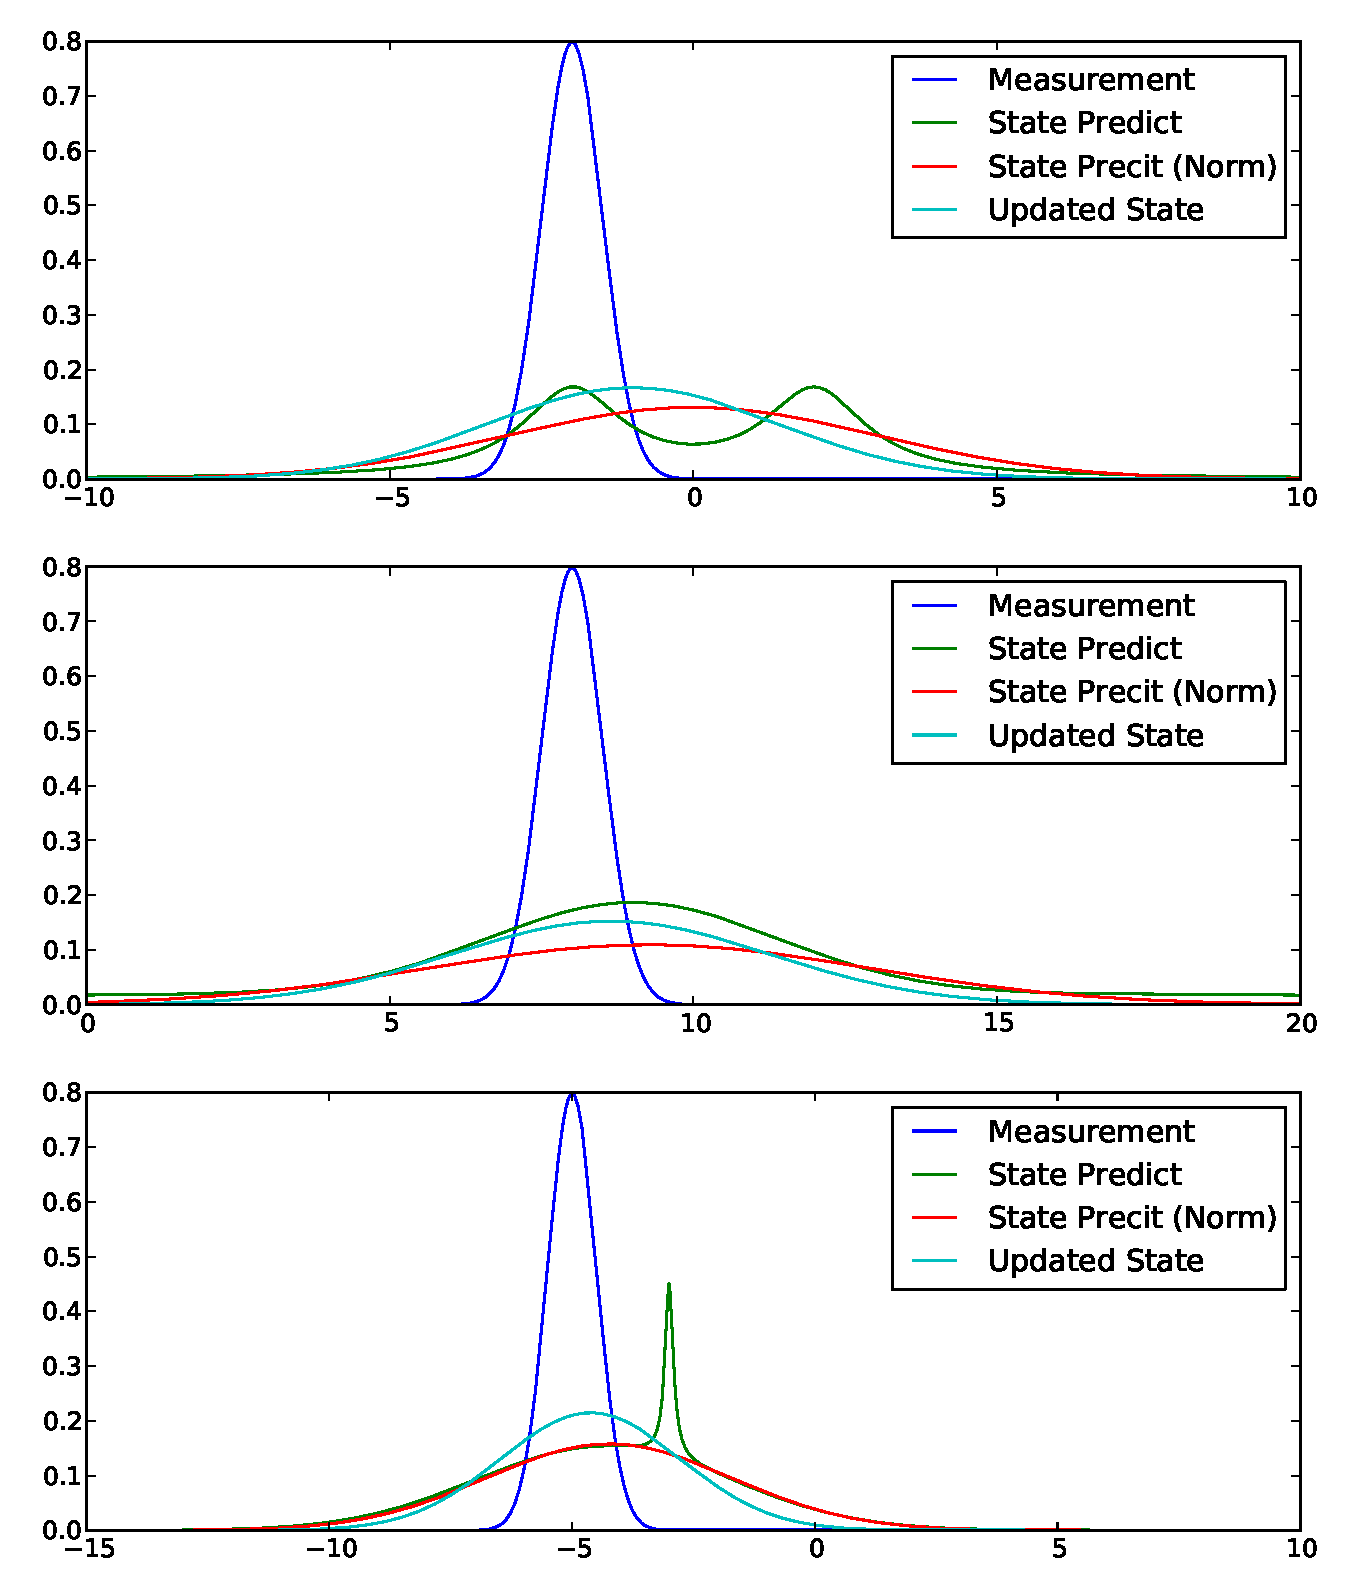
\includegraphics[width=16cm]{images/kalman}
%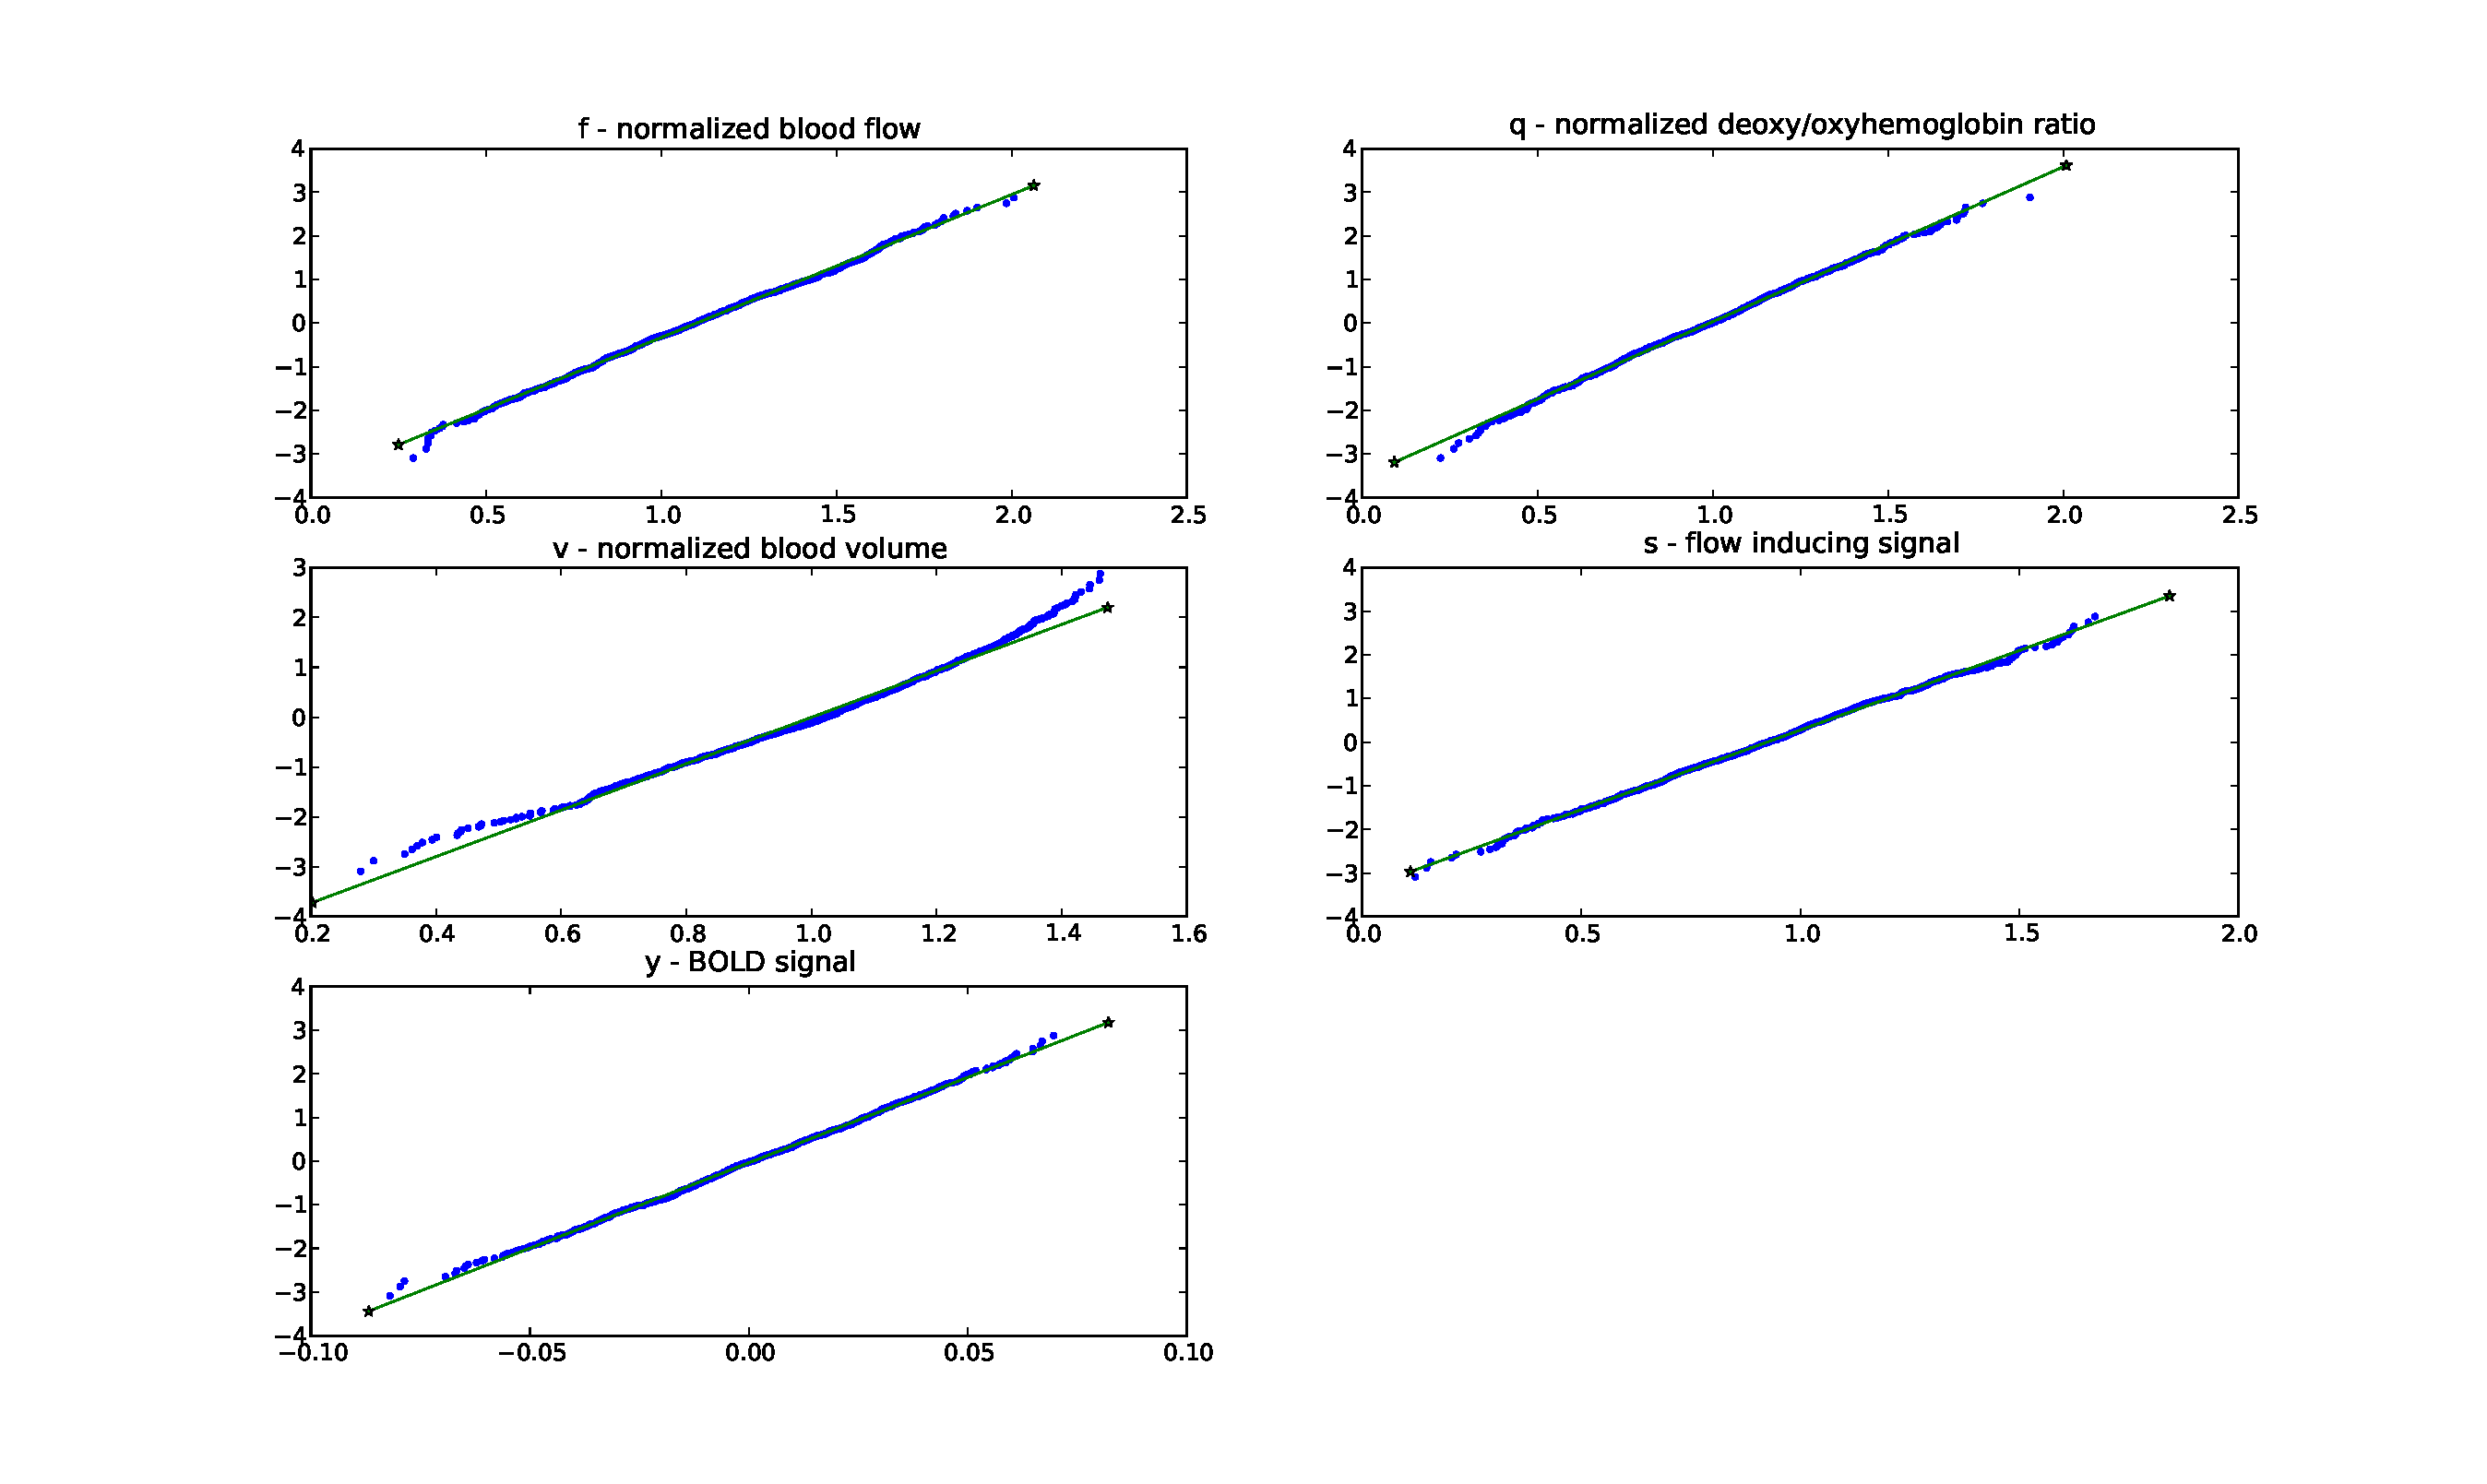
\includegraphics[trim=6cm .75cm 6cm .75cm,width=16cm]{images/gauss_step_point1sec_3sigma.pdf}
\caption{Example updates of a distribution using the Kalman Filter.}
\label{fig:EKFWorking}
\end{figure}

The difficulty
of using a Kalman Filter, however, is that it assumes a multivariate 
Gaussian for the state variables, $X(t-1)$. The more nonlinear the system
gets the more likely that the Gaussian will be insufficient to describe
the distribution, $X(t)$. When this occurs, every step from  $X(t-1)$ 
to $X(t)$ will introduce additional
error in the posterior distribution. Furthermore, it is not really known what 
sort of underlying distributions may exist in such a mixed biological,
mechanical, chemical system such as the brain.
 The assumption of Gaussianity is what allows
the \ac{UKF} to estimate the posterior distribution using only the 
first and second moments;
however, if this assumption is violated significant error will result.
 On the other hand, for
small variances and short time steps the Gaussian distribution is a good 
fit, and so in some cases the Unscented Kalman Filter could work quite
well. 
\begin{table}[t]
\centering
\begin{tabular}{|c || c |}
\hline 
Parameter & Run 1 \\
\hline
$\tau_0$ & .98  \\
$\alpha$ & .33 \\
$E_0$ & .34  \\
$V_0$ & .03  \\
$\tau_s$ & 1.54  \\
$\tau_f$ & 2.46  \\
$\epsilon$ & .54  \\
$V_t$ & N(1, .09)  \\
$Q_t$ & N(1, .09)  \\
$S_t$ & N(1, .09) \\
$F_t$ & N(1, .09) \\
\hline
\end{tabular}
\caption{Parameters used to test Gaussianity of variables after being transitioned through
the \ac{BOLD} model}
\label{tab:steptable} 
\end{table}

To determine the amount of error incurred in a Gaussian estimate during
a typical sample period, the states of \ac{BOLD} equations were assigned according
to a four dimensional Gaussian. The states were then propagated through 
two seconds of simulation (a typical \ac{TR} in \ac{fMRI}) and plotted the resulting
marginal distributions against a Gaussian distribution. This also demonstrates
the degree of nonlinearity present in the system. The parameters used are 
shown in \autoref{tab:steptable}

In order to drive the system without input, the initial state was set
to a non-steady but physically 
plausable $s_t$ state value. The value of $u$ was left at zero 
the entire time, so the 
system would decay naturally (see \autoref{sec:BOLD Physiology})
\autoref{fig:transp1s} shows the results after the
system ran for 100 milliseconds. 
The Q-Q plots fit will with a Gaussian, demonstrating that at this short
time interval nonlinearities have not yet begun to effect the distribution.
However, \autoref{fig:trans1s} shows the result after 1 second, which is faster
than most \ac{fMRI} scanners are capable of sampling at. At that range the tails 
of the distributions for $v$ and $q$ started to deviate from the
Gaussian distribution. As a result the uncertainty in $y$ deviated from
the Gaussian distribution as well. This is important, because although 
approximating the distribution with a Gaussian based on the first two
moments will work in the short run, within a period less than typical
measurement rates the distribution deviated from a Gaussian substantially. 

Thus, even without introducing variation in the model parameters,
a distinct nonlinearity and non-Gaussianity was present. 
More advanced tests where parameters (especially $\alpha$) are varied
would certainly introduce more error into the Gaussian estimate. 
For this reason, estimating the posterior distribution using only 
the first two moments, which is the basis for the \ac{UKF}, is not wise. 

\begin{figure}
\centering
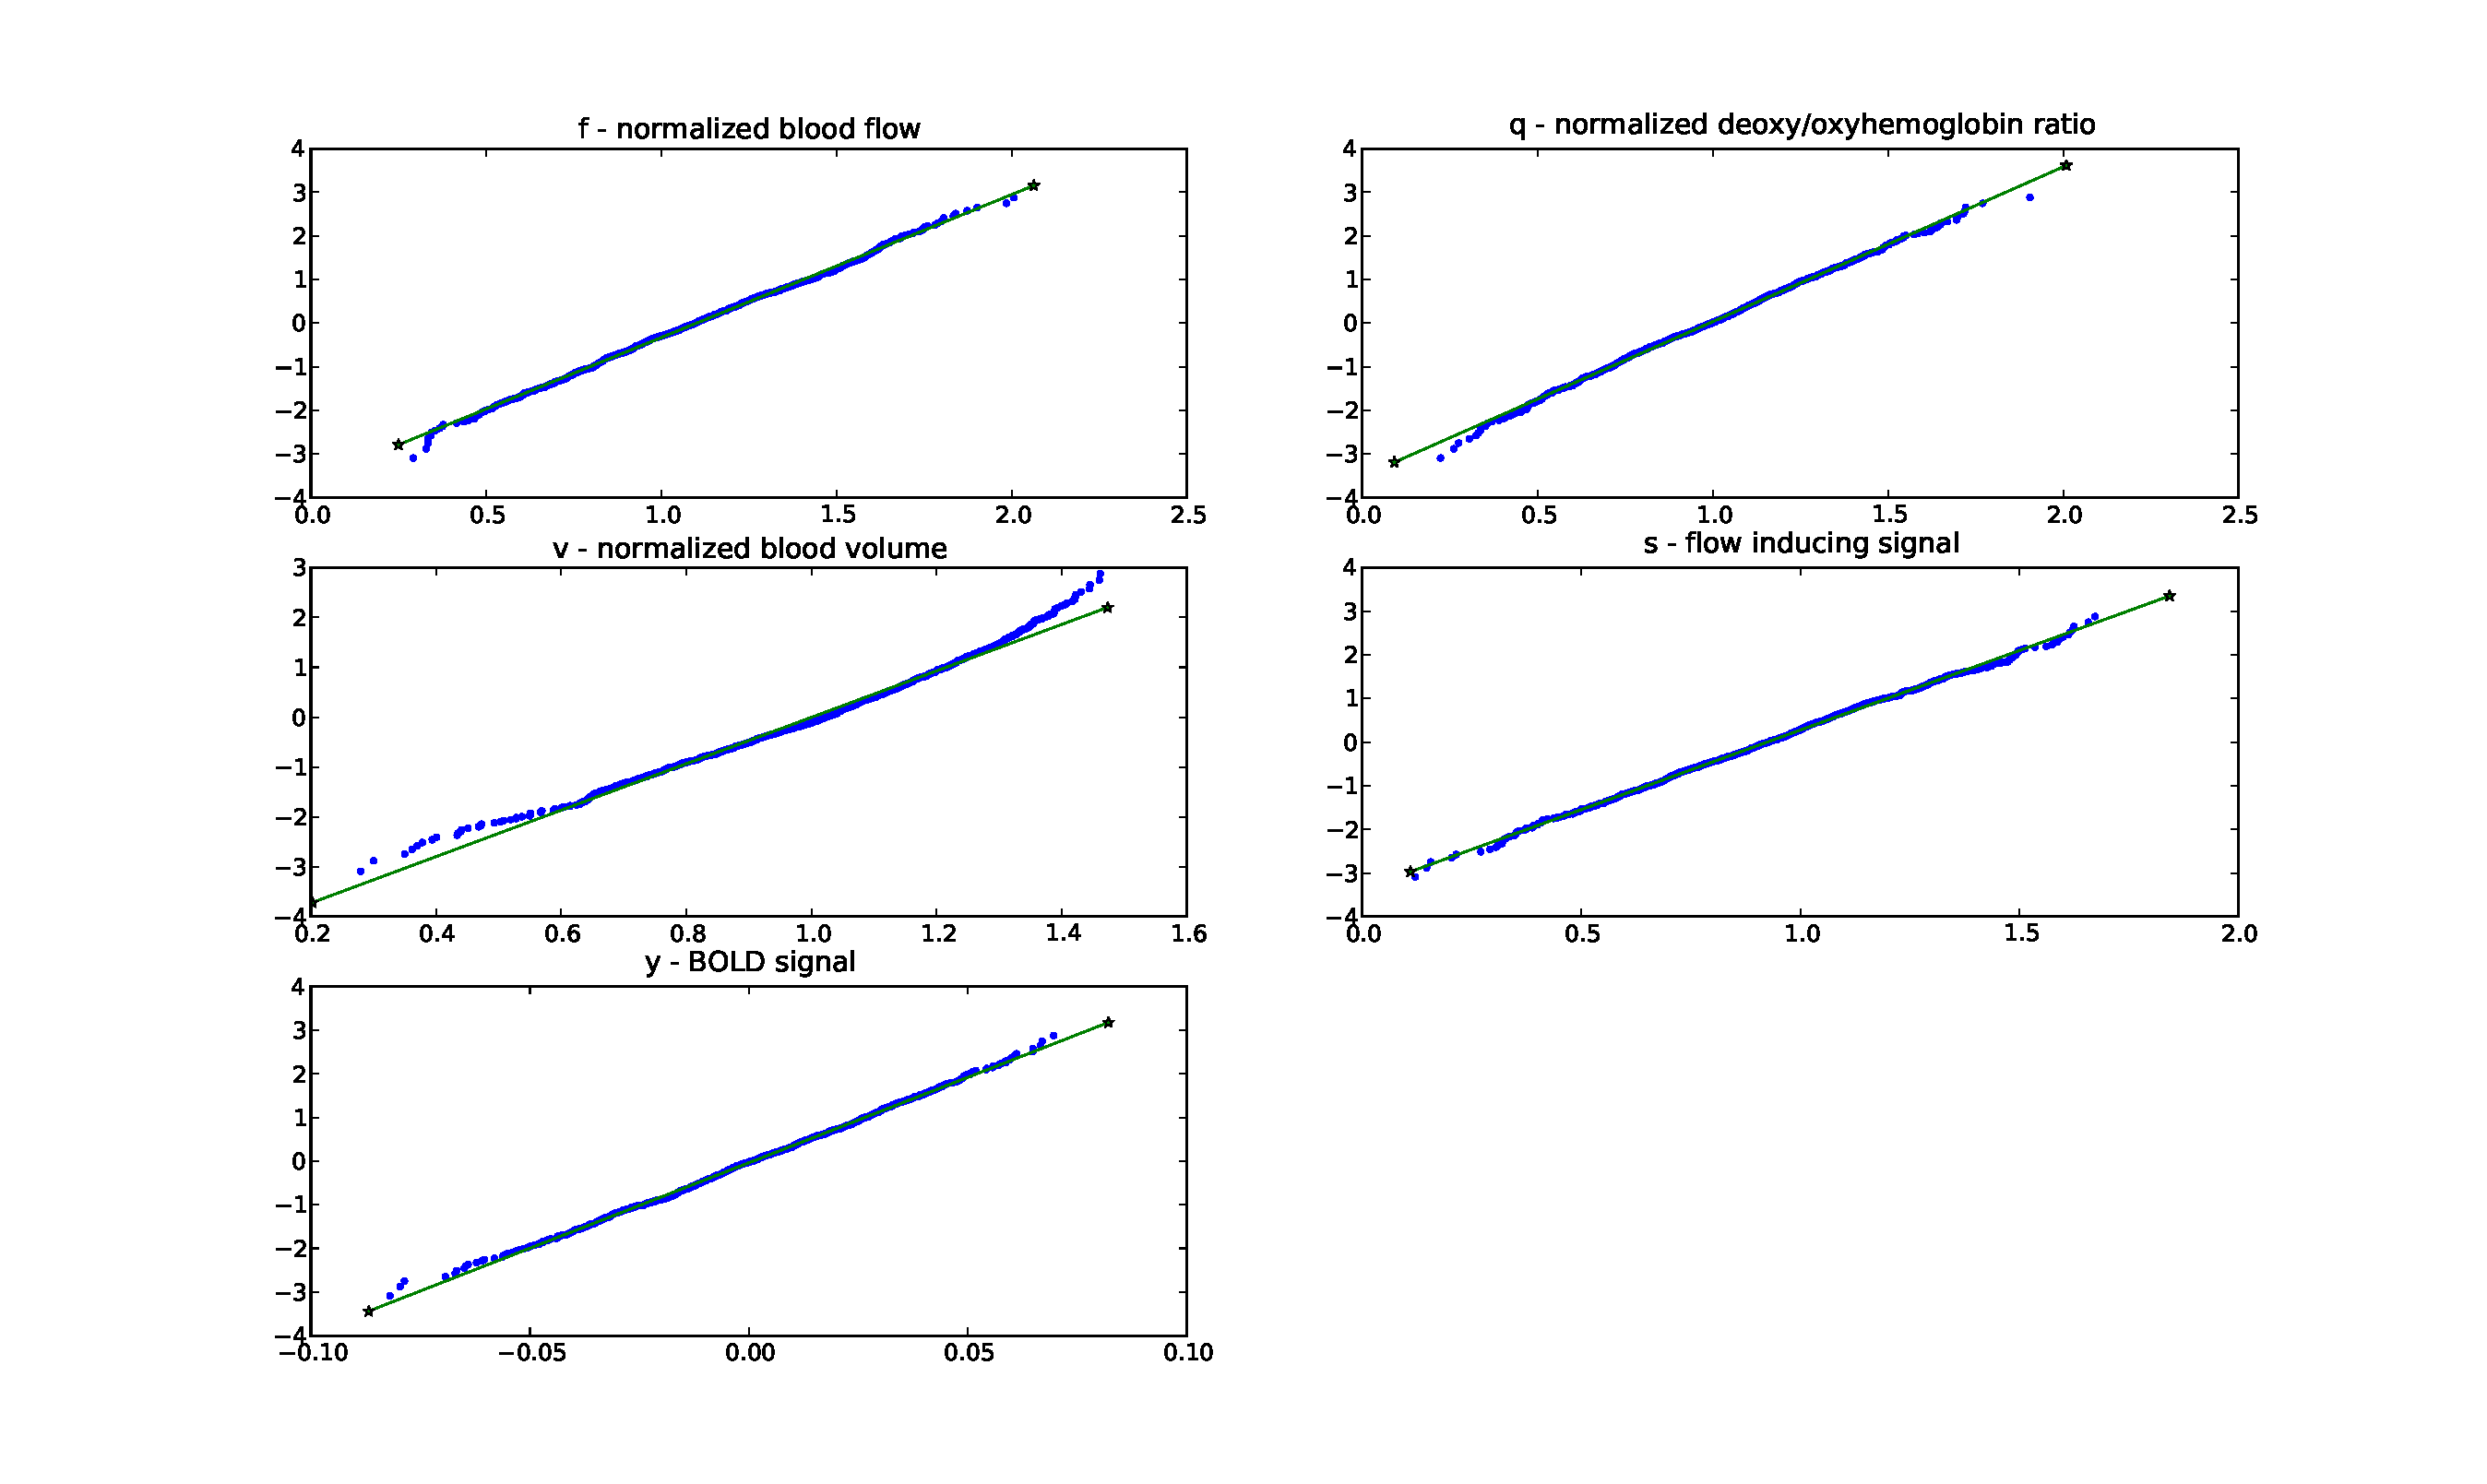
\includegraphics[trim=6cm .75cm 6cm .75cm,width=16cm]{images/gauss_step_point1sec_3sigma.pdf}
\caption{Distributions of state variables after simulating for $0.1$s}
\label{fig:transp1s}
\end{figure}

\begin{figure}
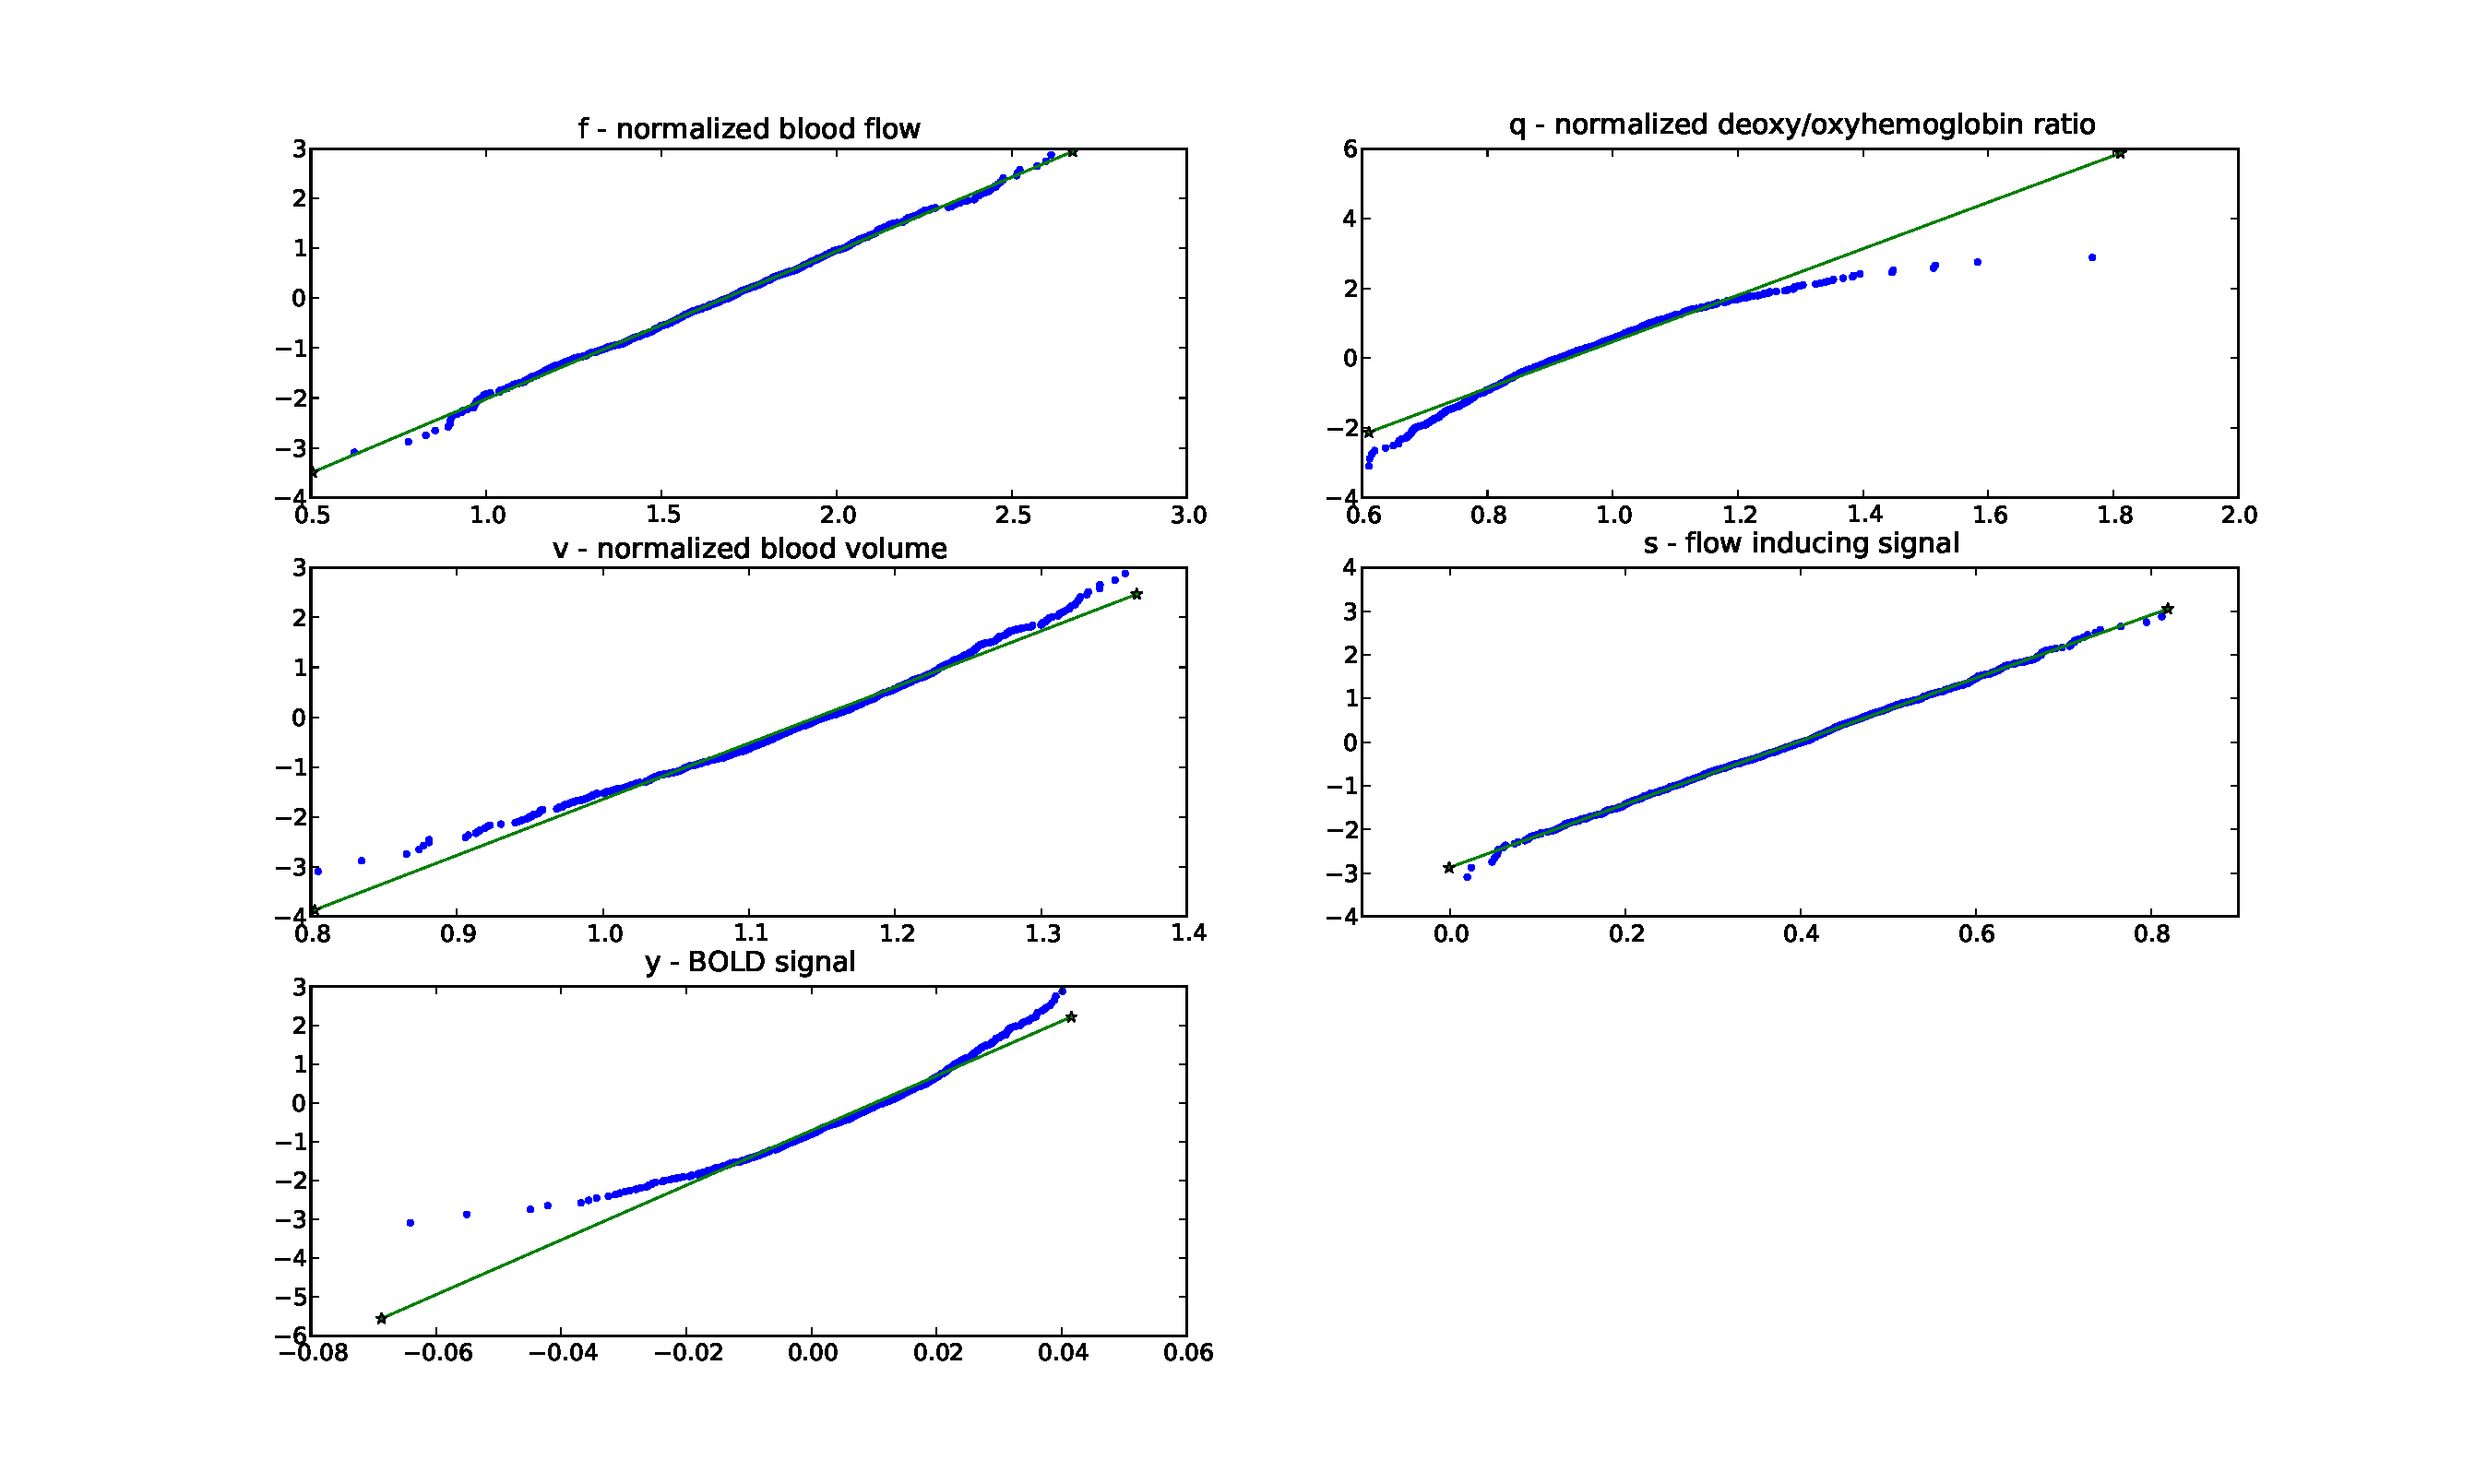
\includegraphics[trim=6cm .75cm 6cm .75cm,width=16cm]{images/gauss_step_1sec_3sigma.pdf}
\caption{Distributions of state variables after simulating for $1$s}
\label{fig:trans1s}
\end{figure}

\subsection{Hybrid Methods}
In Riera et al. \cite{Riera2003}, a maximum
likelihood method for innovation processes was used, as described by
Ozakai \cite{Ozaki1994}. Ozaki \cite{Ozaki1994} used a similar construction to a 
Kalman filter on nonlinear signals \cite{Ozaki1994}. 
The method used by Riera et al.\cite{Riera2003} used this method to 
perform maximum likelihood on
the innovations rather than the absolute signal levels. 
By using a Local Linearization Filter,
innovation noise such as noise in $\dot{f}$ is turned into simple 
Gaussian noise. This approach is useful when the \ac{DC} portion of the signal is
of no use; however, it depends greatly on the type of signal. I found that
this method was not very effective for the \ac{BOLD} signal, when I used it 
with the particle filter approach discussed in the next chapter; although its
effectiveness depended greatly on the stimulus.

In Johnston et al. \cite{Johnston2007}, a hybrid particle filter/gradient
descent algorithm was used to simultaneously derive the static and dynamic 
parameters, (classically known as parameters and state variables, respectively)
.
A particle filter was used to calculate the state variables at each
time; then the estimated distribution of the particles was used to find
the most likely set of parameters that would give that distribution of state variables.
This process was repeated until the parameters converged. Interestingly Johnston et al. \cite{Johnston2007}
came to a very different set of parameter estimates as compared
to the original Friston et al. \cite{Friston2000} estimates (\autoref{tab:Params}).
In fact the results 
are significantly different from virtually every other study. The most obvious discrepancy
is the larger time constants, $\tau_f$, $\tau_s$ and $\tau_0$. 
While of course this could be poor convergence of the algorithm, there is another other possibility.
Unlike all the other methods mentioned, excepting the methods in 
\autoref{sec:Nonlinear Least Squares},
the algorithm described in Johnston et al. \cite{Johnston2007} 
does not depend on prior distributions.
It is possible then that the bias toward the prior in other methods 
skewed their results. 
While Johnston et al. \cite{Johnston2007} is certainly in the minority;
further exhaustive studies 
of the parameters, using unbiased techniques may be called for. A further 
comparison between the distributions found in Johnston et al.
\cite{Johnston2007} and Friston et al. \cite{Friston2000} 
will be discussed in \autoref{sec:PriorDist}. Although Johnston et al.
\cite{Johnston2007} did not explicity list computation times, from
this work, a particle filter with 100 particles integrating the 
BOLD model should take around 5 seconds, repeated 10 times should
take approximately 50 seconds for the particle filter alone. For
the least squares searches performed at each iteration, computation
likely takes around a minute, giving the algorithm a 10 minute 
computation time per voxel. 

In Vakorin et al. \cite{Vakorin2007}, a combination of Genetic Algorithms and 
Simulated Annealing was
used to estimate not only the parameters, but the true stimuli driving the \ac{BOLD}
signal. 
This addresses the inherent uncertainty of exactly where and when 
stimuli actually get applied. Unfortunately this algorithm took
in more than 16 hours per voxel.

\subsection{Previous Particle Filter Approaches}
In his PhD thesis, Murray \cite{Murray2008} used a particle filter based 
approach to integrate
the \ac{BOLD} equations. The method used in that work focused primarily on estimating
the \ac{BOLD} output and state equations as a nonlinear stochastic differential 
equation. The primary difference between that work and this is that
Murray \cite{Murray2008} took the parameters as a given. Thus, differences in the \ac{BOLD} output
were taken to be primarily driven by stochastic changes in the underlying state
equations. Because the parameters were not allowed to change, the estimate of 
the \ac{BOLD} signal was not very good. The fact that the
differences in \ac{BOLD} response cannot be explained solely by stochastic elements 
is important, however. The filtering framework created
in Murray \cite{Murray2008}, dysii, forms the basis for the particle 
filter used in this work, 
and was well designed. The work also clearly presents the particle filter;
both its derivation and use. 

\section{Conclusion}
Currently there is no ideal solution to solving this system of nonlinear
equations. Exhaustive search type methods such as those employed by
Johnston et al. \cite{Johnston2007} and Vakorin et al. \cite{Vakorin2007}
have greater than 10 minute run times for a single voxel. 
While Volterra models are an interesting
solution,there have not yet been exhaustive tests to determine whether
such approximations work well throughout state space. The most promising
method of those reviewed here is the Kalman filter based method. It is
able to maintain a fast runtime while still approaching the solution.
The reliance on a Gaussian estimate to the true posterior distribution could
cause problems however. 
The particle filter method proposed in the next section bears a strong 
resemblance to the unscented Kalman filter; albeit without the Gaussian 
assumptions. 

\chapter{Particle Filters}
\label{sec:Particle Filter}
\section{Introduction}
Particle filters, a type of Sequential Monte Carlo (SMC) methods,
are a powerful way of estimating the posterior probability distribution
a set of parameters given a timeseries of measurements. Unlike Markov 
Chain Monte Carlo (MCMC) estimation, particle filters are designed for 
time-varying random variables. The idea behind particle filters is
extremely similar to Kalman Filters; however, unlike Kalman Filters,
distributions are stored as an empircal distribution rather than the
as the first two moments of a Gaussian. Thus particle filters are 
preferred when the model is nonlinear, and thus non-gaussian.

\section{Model}
\label{sec:Particle Filter Model}
The idea of the particle filter is to build an empirical distribution
out of a large number of parameter \emph{sets}, called particles. Each
particle contains all the parameters and states needed to propagate
the model forward.  The particle filter begins with a wide distribution 
(called the Prior Distribution)
of possible particles and then, as measurements come in, weights 
particles based on the quality of their output estimates. Thus parameter sets 
that tend to give good estimations of the measurements get weighted higher
than parameter sets that give poor estimates. Although the reliance on
a prior distribution can be troublesome, when the system being modeled
has physical meaning, establishing reasonable ranges for parameters can 
actually be quite easy. Optimizing the prior can be more difficult though,
unless the system has been extensively studied.

Suppose set or stream of measurements at discrete times are given, 
$\{Y_k, k = 1, 2, 3, ... K\}$, where $K$ is infinite for a stream. 
Because $k$ is a discrete time, let $t_k$ define the continuous
time of $k$
Suppose also that there is a hidden set of state variables,
$X(t)$ that dictates the movement
of $Y(t)$, although for most of the time dealings will be
with $X_k = X(t_k)$. The goal of the particle filter is to estimate the 
\emph{distribution} of the
true parameters $\Theta$ that dictates the movement of $X(t)$.
The model also permits random motion in $X(t)$, so the 
particle filter also estimates the distribution of $X(t)$.
The only difference between the members of parameter vector
$\Theta$ and those of $X(t)$ is that the memebers of
$\Theta$ have no known update equation. Members of both vectors
are permitted to have some noise, although this
may not be explicitly stated in the model. The generic, continuous, nonlinear
system definition is shown in \autoref{eq:GenericNonlinear}.

\begin{eqnarray}
\dot{X}(t) = f(t, X(t), u(t), \theta, \nu_x) \nonumber \\
Y(t) = g(t, X(t), u(t), \theta, \nu_y)
\label{eq:GenericNonlinear}
\end{eqnarray}

$X(t)$ is vector of state variables, $\Theta$ is a vector of system
constants, $u(t)$ is an input, $Y(t)$ the observation, and
$\nu_x$ and $\nu_y$ are random variates. Although any of these
variables could be a vector, for the sake of simplicity only
$\Theta$ and $X(t)$ will be considered as such. 

Although not necessary for particle filters in general, a few  simplifying
assumptions are made for this work. First, the systems are assumed to be 
time invariant. This 
assumption is based on the idea that if you paused the system for $\Delta t$
seconds, when unfrozen the system would continue as if nothing happend. 
Few biological systems are predictable enough for them to be summarized
by a time varying function, least of all the brain. While heart beats are certainly
periodic and have an effect on the BOLD signal, the period varies too much
for the system to be considered varying with time. 
Next, its assumes that input cannot directly
influence the output, which in the case of the BOLD signal is a good assumption.
Also, noise is considered to be additive.
Finally, because the only difference between the members of $X(t)$ and 
$\Theta$ is an update function, from now on $x$ will contain 
$\Theta$. The assumptions now allow for a simplified version of the
state space equations:

\begin{eqnarray}
\dot{X}_k = f(X_{k-1}, u_k) + \nu_x 
\label{eq:stateass}\\
Y_k = g(X_k) + \nu_y 
\label{eq:measass}
\end{eqnarray}

\section{Derivation}
The goal of the particle filter is to evolve an empirical distribution 
$P(x_k | u_{0:k}, Y_{0:k})$,
that asymptotically approaches the true probability distribution $P(X_k | u_{0:k})$.
Note that capital $X$ will be used as the actual realizations of 
the state variable, whereas $x$ will denote estimates of $X$.
Additionally, the notation $a:b$ indicates the set $[a,b]$,
as in $u_{a:b}$, which would indicate all the inputs from time $a$ to time $b$.
Considering the noise present in $X$,
 $P(X_k | u_{0:k})$ is not a single true value but probability distribution. 

To begin with, the particle filter must be given a prior distribution, from
which the initial $N_p$ particles are drawn. A particle contains a weight
as well as an estimate of $X_k$, which as already stated, contains every
variable needed to run the model. Then the prior is generated from a 
given distribution, $\alpha(X)$, by:

\begin{equation}
\{[x^i_0,w^i] : x^i_0 \sim \alpha(X), w^i = \frac{1}{N_p}, i \in \{1, 2, ... , N_p\} \}
\end{equation}

Where $N_p$ is the number of particles or points used to describe the prior 
using a Mixture PDF. 
Note that any exponents will be explicitly labeled as such, to avoid confusion with
the particle numbering scheme. 

Therefore, after the particle have been generated they should approximate $\alpha(X)$:

\begin{equation}
\alpha(X) \approx P(x_0) = \sum_{i=0}^{N_p} w^i\delta(X - x^i_0 ) dx
\end{equation}
Where $\delta(x-x_0)$ is 1 if and only if $x = x_0$ (the Kronecker delta function).

If a flat prior is 
preferred, then each particle's weight could be scaled to the reciprocal of the
density at the particle: 
\begin{equation}
w^i = \frac{1}{\alpha(x^i_0)}
\end{equation}
Whether or not to flatten the prior is a design decision. The reason this might 
be preferred over a direct
uniform distribution is that the distribution width will inherently scale 
for increased particle counts although some distributions
flatten out better than others. Either way, $\alpha(X)$ \emph{must} be
wide enough to incorporate any posterior that arises. If the prior is
not sufficiently dense, the particle filter can compensate, if it is
not sufficiently wide the particle filter won't converge. 

%todo, put back?
%Once the probability, $P(x_k | x_{0:k-1}, y_{0:k-1})$ has been found
%(initially this is just Mixture approximating the prior since no measurements are 
%available and no previous probabilities are available), its possible to approximate
%the probability between times when measurement is available, by shifting
%the probability according the progression of the state equations. This is only 
%an approximate, since integrating $\nu_d$ should increase uncertainty as
%time without a measurement passes. 
%
%\begin{equation}
%P(x(T+\Delta t)) \approx 
%\sum_{i=1}^{N_p} w_i\delta\left(x - (x_i(T) + \int_T^{T+\Delta} \dot{x}_i(t) dt) \right)
%\end{equation}

\subsection{Weighting}
For all the following areas, the probabilities implicitly depend on $u_{0:k}$, 
so those terms are left off for simplicity.

Whenever a measurement becomes available it permits refinement of the
posterior density.
This process of incorporating new data is called sequential importance sampling,
and eventually allows convergence. The weight is defined as
\begin{equation}
w^i_k \propto \frac{P(x^i_{0:k} | y_{0:k})}{q(x^i_{0:k} | y_{0:k})}
\label{eq:weightfunc}
\end{equation}
where $q$ is called an \emph{importance density}. The importance density
is the density of the points, thus by dividing by this value, the weight
should not depend on the location of the estimation points, but rather
only on $P(x^i_{0:k} | y_{0:k})$, the probability of that particle
being correct given all the measurements up to time $k$. 
Of course if there is a far off peak in
the posterior that $q$ does not have support points in, there will 
be quantization errors, and that part of the density can't be modeled. This is why
it is absolutely necessary that $q$ fully covers $P(x^i_{0:k} | y_{0:k})$.

It is helpful
to consider how the importance density affects the initial distribution. 
In the initial distribution, the weights are all the same; and for
the sake of argument, let them all be scaled up to 1. Then
\begin{equation}
w^i_k q(x^i_{0:k} | y_{0:k}) = q(x^i_{0:k} | y_{0:k}) = P(x^i_{0:k} | y_{0:k})
\end{equation}
the estimated probability, $P(x^i_{0:k} | y_{0:k})$ depends only on the 
way the particles are distributed. As new measurements are incorporated,
the weight will accumulate probabilities through time, which will be discussed
next. 

\section{Calculating Weights}
To calculate the weight of a particular particle, it is necessary to 
calculate both $q(x^i_{0:k} | y_{0:k})$ and $P(x^i_{0:k} | y_{0:k})$.
Note that $q(x^i_{0:k} | y_{0:k})$ may be simplified by assuming that 
$y_k$ doesn't contain any information about $x_{k-1}$. Technically this 
could be false; since later measurements may shed light on currently hidden
changes in $x$. For practical applications though it is helpful assumption.
\begin{equation}
q(x^i_{0:k} | y_{0:k}) = q(x^i_{0:k} | y_{0:k-1})
\label{eq:QAssump}
\end{equation}
The choice of the importance density is another design decision; however
it is common to use the integrated state equations. 
Although other importance density functions exist; for the particle filter
used here, the standard importance density will be used: the modeled
prior.
\begin{equation}
q(x_k | x_{k-1}, y_{0:k}) =  P(x_k | x_{k-1})
\label{eq:ImportanceDensity}
\end{equation}
The benefit of this choice for importance density is that an approximation for
$P(x_k | x_{k-1})$ is freely available: its simply the set of particles propagated
forward in time using the state equations. Additionally it makes
updating weights extremely simple, as seen in \autoref{eq:weightevolve}.

The $q(x^i_{0:k} | y_{0:k})$ may then be simplified:
\begin{equation}
\begin{array}{cclr}
q(x_{0:k} | y_{0:k}) & = & q(x_k | x_{0:k-1}, y_{0:k})q(x_{0:k-1} | y_{0:k}) &  \\
& = & q(x_k | x_{0:k-1}, y_{0:k})q(x_{0:k-1} | y_{0:k-1})  & \text{[\autoref{eq:QAssump}]} \\
& = & q(x_k | x_{k-1}, y_{0:k})q(x_{0:k-1} | y_{0:k-1})  & \text{[Markov Property]}\\
& = & P(x_k | x_{k-1})q(x_{0:k-1} | y_{0:k-1})  & \text{[\autoref{eq:ImportanceDensity}]}
\end{array}
\end{equation}

Calculating $P(x_{0:k} | y_{0:k})$ is a bit more involved. 
First, using the assumption that the distribution of $y_k$ is 
fully constrained by $x_k$, and that $x_k$ is similarly fully 
constrained by $x_{k-1}$, we are able to make the very good assumptions that:
\begin{eqnarray}
P(y_k | x_{0:k}, y_{0:k-1}) &=& P(y_k | x_k) \nonumber \\
P(x_k | x_{0:k}, y_{0:k-1}) &=& P(x_k | x_{k-1})
\label{eq:MarkovProperty}
\end{eqnarray}
These are of course just re-statements of the state equations assumed by \autoref{eq:stateass}
and \autoref{eq:measass}.

Additionally, for the particle filter $y_k$ and $y_{0:k-1}$ are 
constant across all particles, thus $P(y_k| y_{0:k-1})$ can
be dropped when the equality is changed to a proportion. 
Using these properties, $P(x^i_{0:k} | y_{0:k})$ may be broken up as follows 
(mostly using Bayes' Theorem):
\begin{equation}
\begin{array}{lclr}
P(x_{0:k} | y_{0:k}) & = & \frac{P(y_{0:k}, x_{0:k})}{P(y_{0:k})} & \\
 & = & \frac{P(y_k, x_{0:k} | y_{0:k-1}) \cancel{P(y_{0:k-1})}}{P(y_k | y_{0:k-1}) \cancel{P(y_{0:k-1})}} & \\
 & = & \frac{P(y_k| x_{0:k}, y_{0:k-1}) P(x_{0:k} | y_{0:k-1})}{P(y_k | y_{0:k-1}) } & \\
 & = & \frac{P(y_k| x_{0:k}, y_{0:k-1}) P(x_k | x_{0:k-1}, y_{0:k-1}) P(x_{0:k-1} | y_{0:k-1})}{P(y_k | y_{0:k-1})} &  \\
& = & \frac{P(y_k| x_k) P(x_k | x_{k-1}) P(x_{0:k-1} | y_{0:k-1})}{P(y_k | y_{0:k-1})}  & [\text{\autoref{eq:MarkovProperty}}]\\
& \propto & P(y_k| x_k) P(x_k | x_{k-1}) P(x_{0:k-1} | y_{0:k-1}) & [P(y_k|y_{0:k-1}) \text{ is constant}]
 \end{array}
 \label{eq:UpdateBayes}
\end{equation}
Plugging \autoref{eq:ImportanceDensity} and the result of \autoref{eq:UpdateBayes}
into \autoref{eq:weightfunc} leads to:
\begin{eqnarray}
w^i_k & \propto & \frac{P(y_k| x^i_k) \cancel{P(x^i_k | x^i_{k-1})} P(x^i_{0:k-1} | y_{0:k-1})}
                         {\cancel{P(x^i_k | x^i_{k-1})}q(x^i_{0:k-1} | y_{0:k-1})} \nonumber \\
& \propto & w^i_{k-1}P(y_k| x_k) 
\label{eq:weightevolve}
\end{eqnarray}

Thus, by making the following relatively easy assumptions, evolving a posterior
density  requires no knowledge of noise distribution.
\begin{enumerate}
\item $f(t, x(t), u(t)) = f(x(t), u(t))$ and $g(t, x(t), u(t)) = g(x(t))$ 
\item The PDF $q(x_i(0))$ (the prior) fully covers $P(x_i(0))$
\item Markov Property: $P(x_k | x_{0:k-1}) = Pr(x_k | x_{k-1})$
\item $q(x_{0:k-1} | y_{0:k}) = q(x_{0:k-1} | y_{0:k-1})$
\end{enumerate}

\subsection{Basic Particle Filter Algorithm}
From the definition of $w_i$, the algorithm to calculate
an approximation of $P(X(t_k) | Y_{0:k})$ or $P(X(t_k + \delta t) | Y_{0:k})$
is relatively simple.

\begin{algorithm}
\caption{Sequential Importance Sampling}
\begin{algorithmic}
\STATE Initialize Particles:
\FOR{$i$ : each of $N_p$ particles }
    \STATE $x^i_0  \sim \alpha(X)$
    \STATE $w^i_0 = \frac{1}{N_p}$
\ENDFOR
\FOR{$k$ : each measurement}
    \FOR{$i$ : each particle }
        \STATE $x^i_k = x^i_{k-1} + \int_{t-1}^t f(x(\tau), u(\tau)) d\tau $
        \STATE $w^i_k = w^i_{k-1}P(y_k | x_k)$
    \ENDFOR
\ENDFOR
\STATE $P(x(t_k+\Delta t)) \approx 
\sum_{i=0}^{N_p} w^i_k \delta\left(x - (x^i_k + \int_{t_k}^{t_k+\Delta t} f(x(\tau), u(\tau)) d\tau) \right)$
\end{algorithmic}
\end{algorithm}

\subsection{Resampling}
\label{sec:Particle Filter Resampling}
As a consequence 
of the wide prior distribution (required for a proper discretization of a continuous
distribution), there will be many particles with insignificant weights. While this does help
describe the tails of the distribution, it means a lot of computation will be based.
Instead, it would be preferable if most of the computation is spent on the most probable regions.
Ideally the computation time spent on tails would be proportional to the actual size of the
tails. In this case particle locations would match the true posterior and all weights would
be equal.  The case where a large number of the weights have become irrelevantly small
is called "particle degeneracy". In  \cite{Liu1998b}
an ideal calculation of the "effective" number of particles is found based on the 
particles' "true weight". However, given that only an approximation for the true weight 
exists, they also provide a simple heuristic calculation of $N_{eff}$.
\begin{equation}
N_{eff} \approx \frac{\sum_{i=0}^{N_p} w_i}{\sum_{i=0}^{N_p} w_i^2}
\label{eq:neff}
\end{equation}
Any quick run of a particle filter will reveal that unless the prior is particularly accurate,
$N_{eff}$ drops precipitously.  To alleviate this problem
a common technique known as resampling may be applied. The idea of resampling is to 
draw from the approximate posterior, thus generating a replica of the posterior with 
a better support. Therefore, a new set of particles may be drawn from the empirical
distribution as follows:
\begin{equation}
\hat{x}_j \sim \left(\sum_{i=0}^{N_p} w^i_k\delta(x - x^i_k)\right)
\end{equation}

\begin{algorithm}
\caption{Stratified Resampling Algorithm}
\begin{algorithmic}

\end{algorithmic}
\end{algorithm}

Unfortunately, this isn't necessarily the truth: since the support is
still limited to the original particles, the number of unique particles can only go down.
This effect, often dubbed "particle impoverishment" can result in excessive quantization
errors in the final distribution. However, there is a solution. Instead of sampling from the
discrete distribution, a smoothing kernel is applied, and $\hat{\chi}_j$ are drawn from
that distribution. Because the distribution is continuous, there is no way for a collapse
of the particles to occur. The question then, is how to decide on the smoothing kernel. 
Often times the easiest way to sample from the continous distribution is to break the 
re-sampling down into two steps. First a member of the discrete distribution is randomly
selected based on the weights, and then based on the smoothing a nearby state variable 
is selected. The process of the selection will be defined as:
\begin{equation}
\chi_i = x_i + h\sigma \epsilon
\end{equation}
Where $h$ is the bandwidth, $\sigma$ is the standard deviation such that $\sigma \sigma^T = cov(x)$
and $\epsilon$ is drawn from the chosen kernel.
It has been proven that when all the elements of the mixture
have the same weight, as is the case after basic resampling, the kernel that minimizes the 
MSE between the estimated and true posterior is the Epanechnikov Kernel (cite Improving Regularised
Particle Filters, C Musso, N Oudjane and F LeGrand). 
\begin{equation}
K = \left\{
\begin{array}{lr}
\frac{n_x+2}{2c_{n_x}}(1-\|x\|^2) & if\ \|x\| < 1\\
0 & otherwise
\end{array}\right.
\end{equation}
%<more here>

\subsection{Weighting Function}
Because $P(y_k | x(T))$, what I will call the weighting function,
is based on an unknown distribution, it is necessary to decide on a function
that will approximate $P(y_k | x(T))$. Obviously the function, $\omega(y_k, f(x(t))$
needs to be centered at zero and have a scale comparable to the signal levels.
Obviously if the actual noise present in $y_k$ were to be known, then that would
be the best distribution for $\Omega$. In that case, particles that fell
far out on that distribution would be statistically impossible representations
of the system, and it would be completely reasonable to throw such particles away.
While a Gaussian function is the natural choice, because this distribution
and weight are unknown we wanted to try distributions
with wider tails, so that outliers don't completely destroy particle's weights
(and thus convergence proceeds more slowly).

Another natural choice might be one of the robust estimator weight functions, for
example the Huber or bi-square. For the purpose of this work we will stick
with long tailed distributions, however it is worth noting that long tails
may not be the optimal choice in all, or even this situation. The justification
for long tailed distributions is that we believe the noise to be long tailed,
and the variance of the noise is not well known.

Therefore, we tried three weighting functions based on three distributions: Gaussian, 
Laplace and the Cauchy. The standard deviation of the distribution is extremely
important to the convergence of particle filter. A standard deviation that is 
too large will not allow the distribution to converge in any reasonable number of 
measurements. A standard deviation below the standard deviation of the noise 
will cause the algorithm to throw out perfectly acceptable particles. 
The weighting function ultimately will shape the output distribution, $P[y]$, into that
distribution, however the distribution of $x$ will still approach a reasonable
estimate of its true distribution. Even an overly wide weighting function, will
allow the Gaussian Mixture estimate of $X$ to converge to the correct location 
parameters of the "real" posterior distribution, though the scale parameters may 
be overly large.

A reasonable method of setting the standard deviation of $\Omega$ may be by 
taking a small sample from "resting" data and using the sample standard deviation.
Since this is the first attempt at using particle filters for modeling the 
BOLD model, in this work we set the standard deviation manually at <weight standard dev>,
because it gives a more consistency and control. Of course this could be taken
further, by testing the sample data against a set of stock distributions
and choosing the best fit. This of course depends on having enough samples
to make a reasonable inference, which may not always exist. 

\section{Simple, Nonlinear Example}
A typical half wave rectifier takes a AC voltage circuit and removes
one half (say the negative half) of the signal. The resulting waveform
is still not DC, however it is then possible to use a capacitor to 
smooth the signal into something similar to DC, as shown in \autoref{fig:HalfWaveIO}.
There are other, more
complex circuits that convert the negative portion into positive and
waste less energy but but here we will keep the system simple.
Thus, let us consider a simple half wave rectifier circuit, shown in 
\autoref{fig:HalfWaveRectifier}.

The half wave rectifier circuit smoothes the gaps between high voltage
with a capacitor. Thus, when $u(t)G$ is less than $v_t$, the circuit will 
discharge the capacitor and maintain a non-zero voltage,
but when $u(t)G$ is greater than $v_t$, the output voltage will be set
by $u(t)G$ and the capacitor will charge up. We will assume a very simple
model for all the components, ignoring the complex nonlinear behavior
that can occur in a diode. 

\begin{figure}
\centering
\begin{circuitikz}[scale=2, american]
\draw
 (0,0)  node[transformer core] (T) {}
 (T.A1) -- (-1,0)
 (T.A2) -- (-1,-1.05)  to[V, v=$u(t)$] (-1, 0)
 (T.B1) -- (.5, 0) to[D, l=$v_t$] (1.5,0) to[C=$C$] (1.5, -1.05)
 (1.5, 0) -- (2.5, 0) to[R=$Rm$, v=$v_y$] (2.5, -1.05) -- (T.B2) 
 (T.base) node {G}
 (T.B1) to[open, *-*, v=$V_1$] (T.B2); 
\end{circuitikz}
\caption{An Example Half Wave Rectifier Circuit, where $G$ is the transformer
gain, $v_t$ is the activation voltage of the diode, $u(t)$ is the input at time $t$, 
$C$ is the capacitance, $R$ is the load resistance and $v_y$ is the output voltage}
\label{fig:HalfWaveRectifier}
\end{figure}

\begin{figure}
\centering
\caption{Example Input/Output of the Half Wave Rectifier}
\label{fig:HalfWaveIO}
\end{figure}

Although rectifiers are typically thought
of as receiving an AC circuit 60 Hz, we will ignore such specifics and 
assume the voltage across the output of the transformer is simply a scalar
multiple of the input voltage.  As discussed in the \autoref{sec:Particle Filter Model}
any variable with uncertainty must be part of the state variable. Therefore
the state variable will be: $X(t) = \{G, v_t, C, R_m, v_y\}$. Of course,
$u(t)$ cannot be allowed to be a square wave in such a system, since that
such a signal would never get across the transformer and regardless it
would necessitate an unrealistic infinite current across the capacitor.
The state equations would then be 

\begin{equation}
v_y(t)  = f(v_y(t-1, u(t)) =  \begin{cases} 
        u(t)G & \text{ if }  u(t)G-v_y \ge v_t\\
        v_y(t-1)\left(1 - \frac{\delta t}{R_mC}\right) & \text{ if }  u(t)G-v_y < v_t
    \end{cases} 
\end{equation}

To run the particle filter is relatively easy then, since there exists 
a recursive definition of the dynamic state variable, $v_y$. To start
with, an initial distribution must be assumed and while at first a 
Gaussian seems like a good idea, all the static state variables are strictly
positive and thus not well suited to the Gaussian. In this case then,
it would be wise to start with a Gamma distribution, and just be wary of
any standard deviation that gets larger than the prior mean. We will define
the gamma distribution as follows:

\begin{equation}
X \sim Gamma(k, \theta) \rightarrow f(x) = x^{k-1}\frac{e^{-x/\theta}}{\theta^k\Gamma(k)}
\end{equation}

where $\Gamma$ is the gamma function.
The in some ways the margin for error is decided by the weighting function, which
here will define as $W(V_y, v_{yi})$, where $V_y$ is the actual measurement, $v_y$ is the 
estimate based on all the particles, and 
$v_{yi}$ is the estimate by a particular (i$^{\text{th}}$) particle. The choice of this function is difficult,
and although the Gaussian is typically used, we found the exponential helpful
in dealing with particle deprivation.  The algorithm will then look like the following,

\begin{algorithmic}
\STATE Initialize $N_p$ Particles:
\FOR{$i$ in $N_p$}
    \STATE $G \sim Gamma(\frac{\mu^2_G}{\sigma^2_G}, \frac{\sigma^2_G}{\mu_G})$
    \STATE $v_t \sim Gamma(\frac{\mu^2_{v_t}}{\sigma^2_{v_t}}, \frac{\sigma^2_{v_t}}{\mu_{v_t}})$
    \STATE $C \sim Gamma(\frac{\mu^2_C}{\sigma^2_C}, \frac{\sigma^2_C}{\mu_C})$
    \STATE $R_m \sim Gamma(\frac{\mu^2_R}{\sigma^2_R}, \frac{\sigma^2_R}{\mu_R})$
    \STATE $v_y = 0$, (Assume the system has been off for a long time)
    \STATE let $X_i(0) = \{G, v_t, C, R_m, v_y\}$
    \STATE let $w_i(0) = 1$ or to make a flat prior, $w_i(0) = \frac{1}{Pr(X_i(0))}$ 
\ENDFOR
\STATE Run the Filter:
\FOR{$t$ in Set of Measurement Times}
    \FOR{$i$ in $N_p$}
        \STATE $v_{yi}(t) = f(v_{yi}(t-1), u(t))$
        \STATE (All other members of $X_i(t)$ remain the same)
        \STATE $w_i(t) = w_i(t-1)W(V_y(t), v_y(t))$
    \ENDFOR
\ENDFOR
\end{algorithmic}

Initially the particles will have the same output, $0$, however, as $u(t)$
changes, the response of each particle to that input will result in different
outputs. Particles that have a $v_{yi}$ near $V_y$ will be weighted higher,
and others farther away will be weighted lower. As the particle filter
runs, weights will compound resulting in a distribution that asymptotically
approaches the true joint distribution of the $X(t)$.  Of course, as we
mentioned in \autoref{sec:Particle Filter Resampling}, particles weighted zero do not significantly
contribute to the empirical distribution, so re-sampling may be necessary.
If the noise is assumed to be Gaussian then it is possible to further optimize. 
Thus we let $h$ be defines as:
\begin{eqnarray}
h = [N_s8c^{-1}_{n_x}(n_x + 4)(2\sqrt{\pi})^{n_x}]^{\frac{1}{n_x +4}}
\end{eqnarray}
and although it is very possible the underlying noise is non-gaussian, the Gaussian
may work, but sub-optimally. It has been proposed that (Monte Carlo Approximations for
General State-Space Models, markus Hurzeler and Hans R. Kunsch) if the underlying 
distribution is non-Gaussian, then using this bandwidth will oversmooth. 
In reality over smoothing
should not be too great an issue because the smoothing is only being applied to find new
particles. If the distribution is over smoothed then the algorithm may not converge as rapidly;
however, because the bandwidth is still based on particle variance, which will decay as 
particles are ruled out, it is still able to converge. In fact over smoothing is preferrable
to under smoothing, since the latter would result in false negatives, but the previous only
results in a slower decay of the variance. 
At the same time, as $n_x$, the number of dimensions in
$x$, goes to infinity, the standard deviation based approximation becomes less effective
(cite a Tutorial on Particle Filters for on-line non-linear non-gaussian bayesian
tracking, sanjeev arulampalam, simon maskell, neil gordon...).  Because of the high dimensionality of our system,
and limited measurements, it is helpful to have a broader bandwidth to explore the distribution. 
Nevertheless, because 
of the potentially wide smoothing factor applied by regularized resampling, performing this
step at every measurement would allow particles a great deal of mobility. This mobility is
the enemy of convergence, which is why regularized resampling should only be done when
$\hat{N}_{eff}$ drops very low (say less than 50). Other than the periodic regularized
resampling then, the regularized particle filter is nearly identical to the basic sampling
importance sampling filter (SIS). 

 \begin{algorithmic}
\STATE Initialize $N_p$ Particles: 
        $\{x_i(0),w_i(0) : x_i(0) \sim \alpha(x), w_i(0) = \frac{1}{N_p}, i \in \{1, 2, ... , N_p\} \}$
\STATE $T$ = \{Set of Measurement Times\}
\FOR{$t$ in $T$}
    \FOR{$i$ in $N_p$}
        \STATE $x_i(t) = x_i(t-1) + \int_{t-1}^t f(x(\tau), u(\tau)) d\tau $
        \STATE $w_i(t) = w_i(t-1)P(y(t) | x(t))$
    \ENDFOR

    \STATE Calculate $N_{eff}$ with \autoref{eq:neff}
    \IF{$N_{eff} < N_R$ (recommend $N_R = min(50, .1N_p)$ )}
        \STATE Calculate empirical $\sigma$ 
        \STATE $h = [N_s8c^{-1}_{n_x}(n_x + 4)(2\sqrt{\pi})^{n_x}]^{\frac{1}{n_x +4}}$
        \STATE Redraw particles using (stratified) basic resampling
        \FOR{$i$ in $N_p$}
            \STATE Draw $\epsilon \sim K$
            \STATE $x_i = x_i + h \sigma \epsilon$
        \ENDFOR
    \ENDIF
\ENDFOR

\STATE At $t + \Delta t$, $t \in T$, $P(x(t+\Delta t)) \approx 
\sum_{i=1}^{N_p} w_i(t)\delta\left(x - (x_i(t) + \int_t^{t+\Delta t} f(x(\tau), u(\tau)) d\tau) \right)$

 \end{algorithmic}

The ultimate effect of this regularized resampling is a convergence similar to simulated annealing
or a genetic algorithm. Versions of $x$ that are "fit" (give good measurements) spawn more children 
nearby which allow for more accurate estimation near points of high likelihood. 
As the variance of the estimated
$x$'s decrease, the radius in which children are spawned also decreases. Eventually the radius
will approach the width of the underlying uncertainty, $\nu_x$ and $\nu_y$.


\chapter{Methods}
\label{sec:Methods}
Although the particle filter  is a standard Regularized
Particle filter, as described in \cite{Arulampalam2002a}, optimizing the 
particle filter for use with FMRI data is non-trivial. 


\section{Model}
As originally written in \autoref{sec:BOLD Physiology} the state variables
for the BOLD model are as follows:
\begin{eqnarray}
\dot{s} &=& \epsilon u(t) - \frac{s}{\tau_s} - \frac{f - 1}{\tau_f} \\
\dot{f} &=& s\\
\dot{v} &=& \frac{1}{\tau_0}(f - v^\alpha)\\
\dot{q} &=& \frac{1}{\tau_0}(\frac{f(1-(1-E_0)^f)}{E_0} - \frac{q}{v^{1-1/\alpha}})
\end{eqnarray}
The original assumption regarding particle filter models (\autoref{sec:Particle Filter Model})
included noise in the update of $x$, however that is not included here.
The reason for the difference is that cloud of particles is, to some extent,
able to account for that noise. It is common, however, to model that noise
in particle filters by adding a random value to each updated state variable. 
Because the purpose of this particle filter is to learn the underlying distribution
of the static parameters, rather than precisely model the time course of the 
in the dynamic parameters ($\{s,f,v,q\}$) this noise is left out. It also helps
that detrending is applied before the particle filter and that the
BOLD model is dissipative. When no stimuli are applied, all the particles 
decay to ($\{0,1,1,1\}$). Typical particle filters 
also use this state noise as an exploratory measure; however this method is
less necessary when good priors are available.

Typically a step size of .001 was used, after finding that even .01 can
at times lead to the state equations careening out of control.



\section{Preprocessing}
\label{sec:Methods Preprocessing}
The normal pipeline for analyzing
FMRI involves a several preprocessing steps. The first and most important
task is motion correction. To do this, a single volume in time is chosen, and
volumes at every other time are registered to this one volume. This corrects
for motion by the patient as well as small changes in the magnetic
fields that cause the image to shift. 
In conventional statistical parametric mapping, a Gaussian smoothing
filter is applied across the image as discussed in \autoref{sec:RFT}.
After this, detrending is performed which is discussed in \autoref{sec:Detrend}.
Recall that FMRI signal levels are unit-less and though detrending is not
always necessary, the data must always be converted 
into \% difference from baseline. 
The generally accepted method is to use a high pass filter, although the
cutoff frequency is application dependent and often applied haphazardly.
Before going into the detrending used in this work, it is necessary to 
discuss the type of noise present in FMRI.

\subsection{BOLD Noise}
\label{sec:Introduction Noise}
As demonstrated in \autoref{sec:BOLD Physiology} the BOLD response has been
extensively studied and despite minor discrepancies, the cause of the BOLD 
signal is well known. However, as FMRI detects an  
aggregate signal over the space of cubic centimeters, there are
plenty of noise sources . Though local neurons act
together (i.e. around the same time), the density of neurons, the
density of capillaries, and slight differences in activation across 
a particular voxel can all lead to signal attenuation and noise. 

A particularly difficult form of noise present in FMRI is a low frequency
drift, often characterized as a Wiener process (\cite{Riera2004}). 
Though not present in all regions, as many as ten to fifteen percent
of voxels can be affected (\cite{Tanabe2002}), thus it is prevalent enough to cause significant
inference problems \cite{Smith2007}. It is still not
clear what exactly causes this noise, although one possibility is 
the temperature difference in scanner magnetic coils\cite{Smith2007}. 
It is clear that this drift signal is not solely
due to a physiological effects, given its presence in cadavers and phantoms 
\cite{Smith1999}. Interestingly, it is usually spatially correlated, and
more prevalent at interfaces between regions. Though one potential source
could be slight movement, co-registration is standard, making this unlikely. 
Regardless, the problem mandates the use of a high pass filter \cite{Smith2007}.

In order to characterize the noise, I analyzed resting state data.
During resting state, the patient is shown no images, and he is asked
to avoid movement and complex thought.  Overall though there should be 
very little activation, and thus the signal consists entirely of noise. 
Therefore resting state data is perfect for analyzing noise. 
The locations were chosen from points all around the brain, 
all in grey matter voxels. These time
series were chosen because they were representative of different types
of noise found in the resting state data.

TODO give scanner details

\begin{figure}
\centering
\subfigure[]{\label{fig:QQDC:A}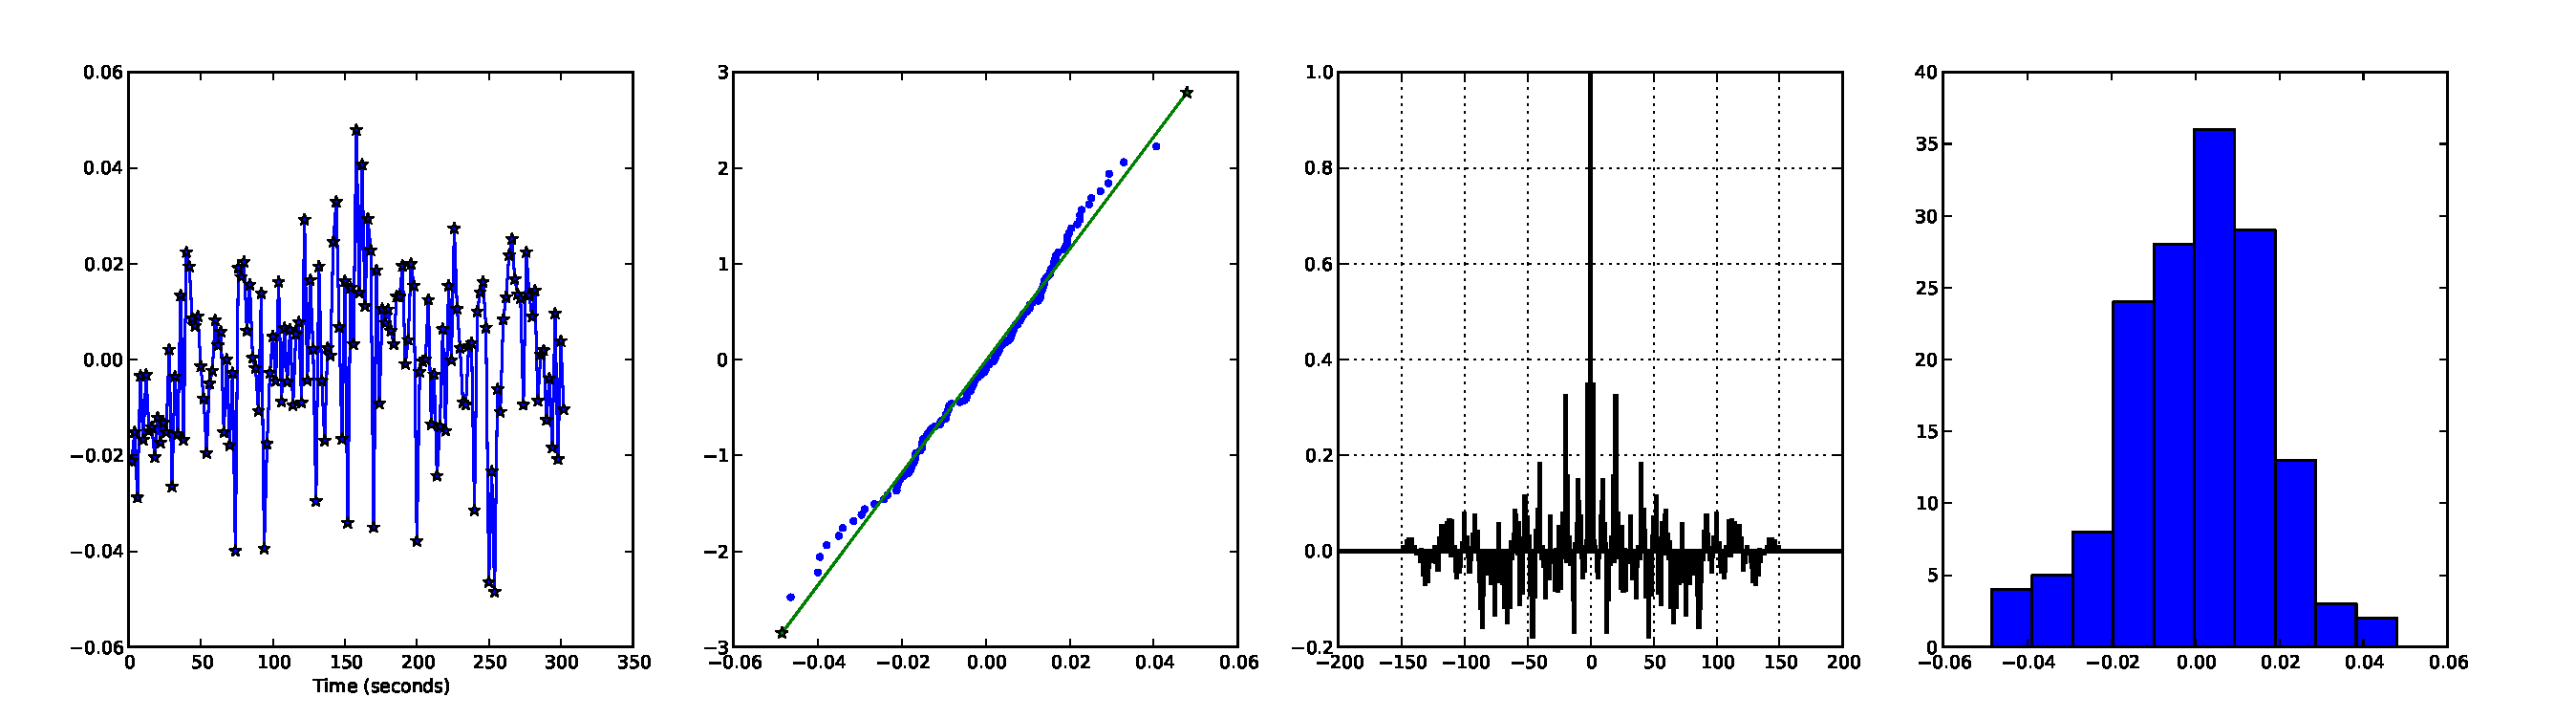
\includegraphics[trim=6cm 1cm 6cm 1cm,width=13cm]{images/noise2_0009_29_49_9}}
\subfigure[]{\label{fig:QQDC:B}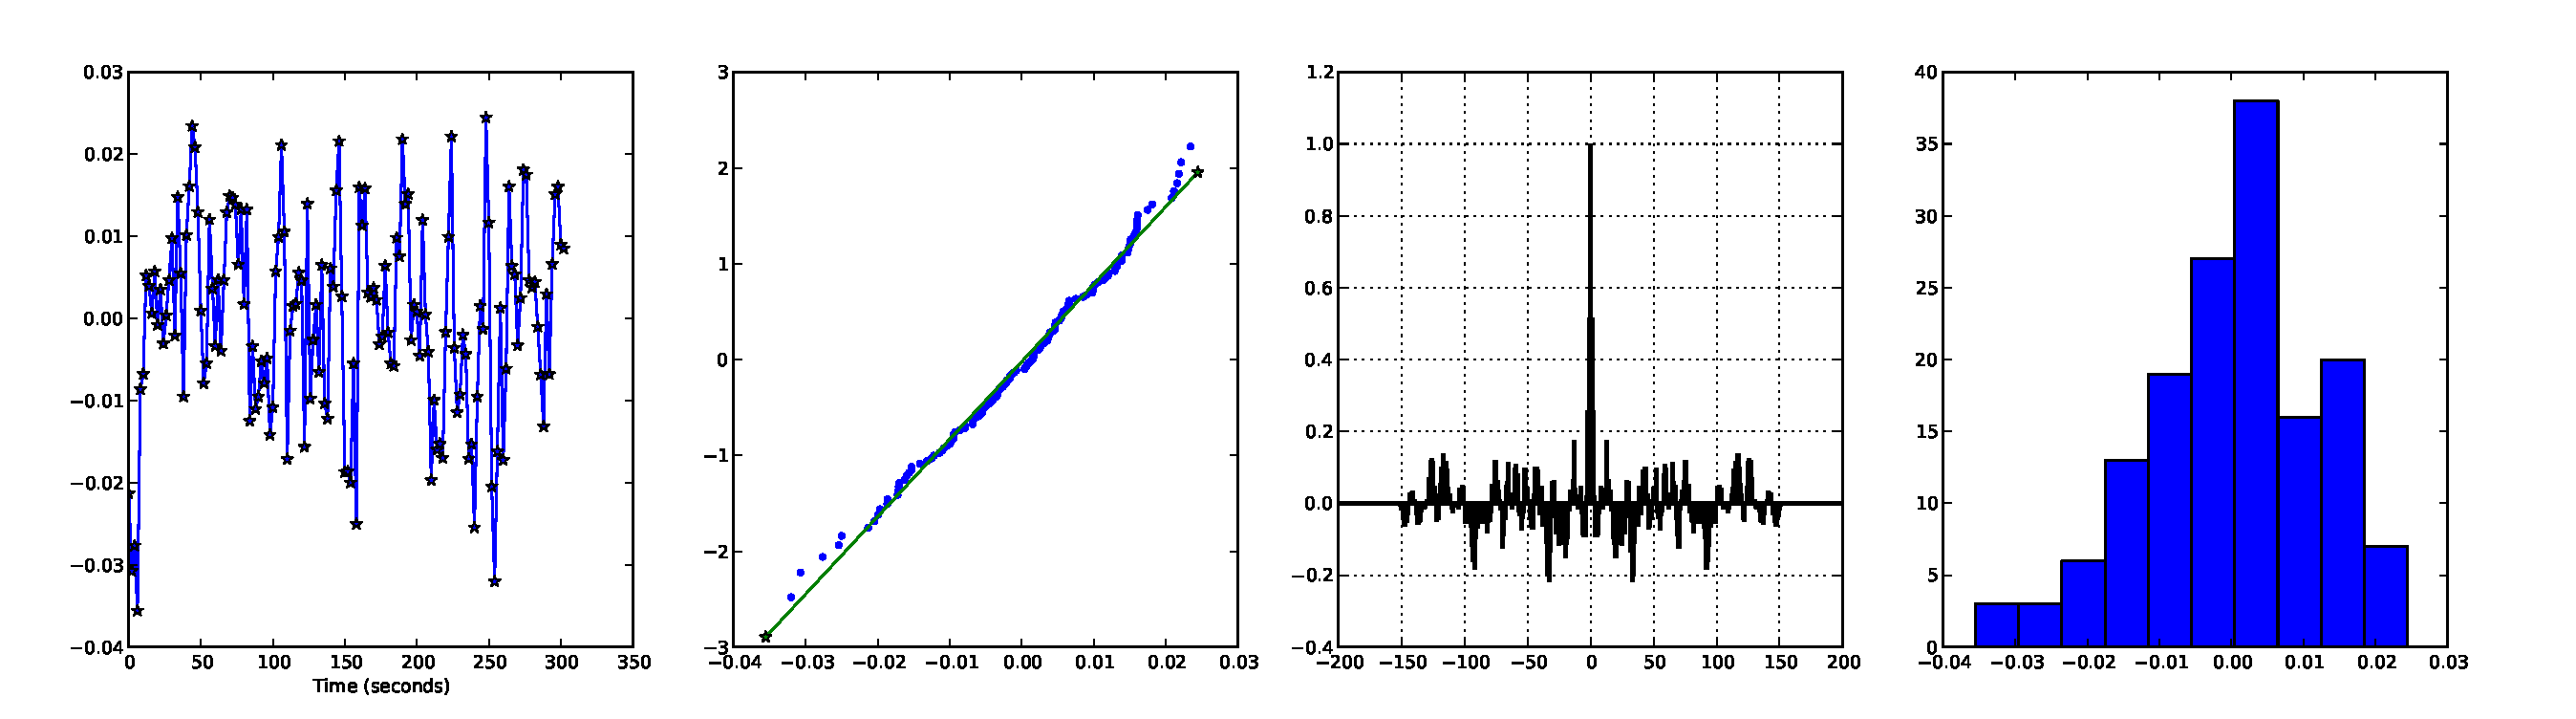
\includegraphics[trim=6cm 1cm 6cm 1cm,width=13cm]{images/noise2_0009_34_43_24}}
\subfigure[]{\label{fig:QQDC:C}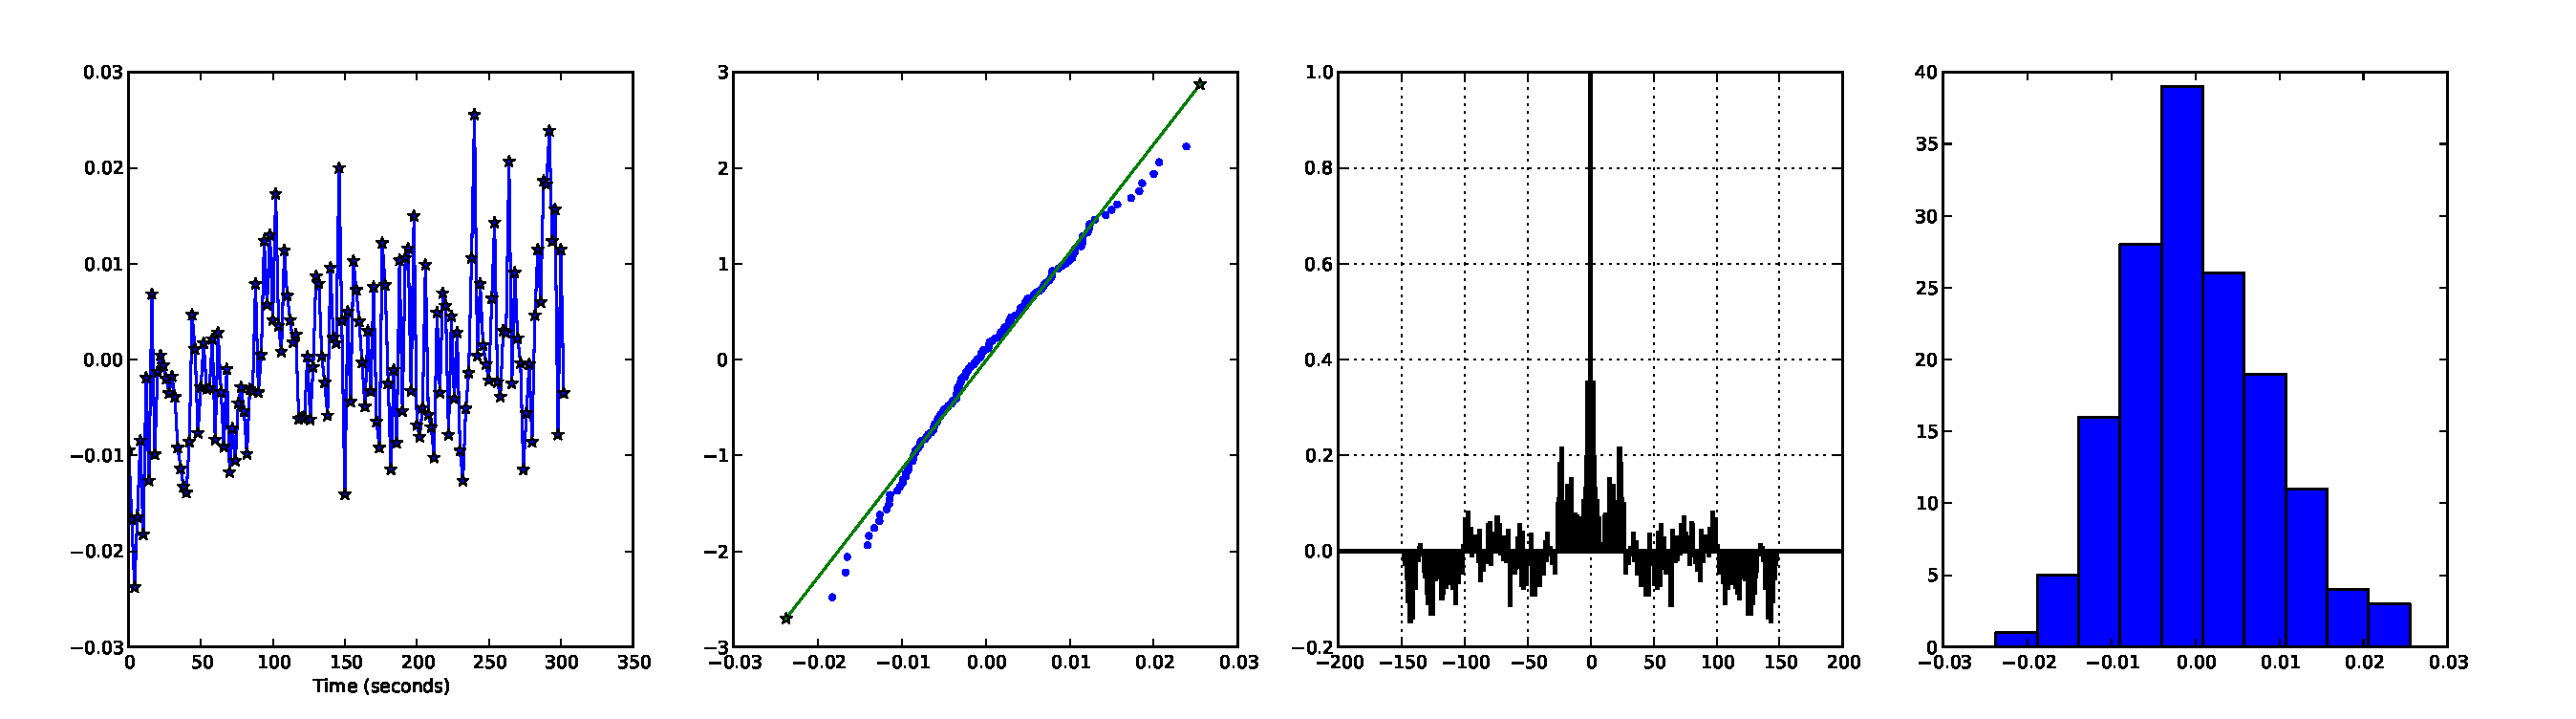
\includegraphics[trim=6cm 1cm 6cm 1cm,width=13cm]{images/noise2_0009_22_38_23}}
\subfigure[]{\label{fig:QQDC:D}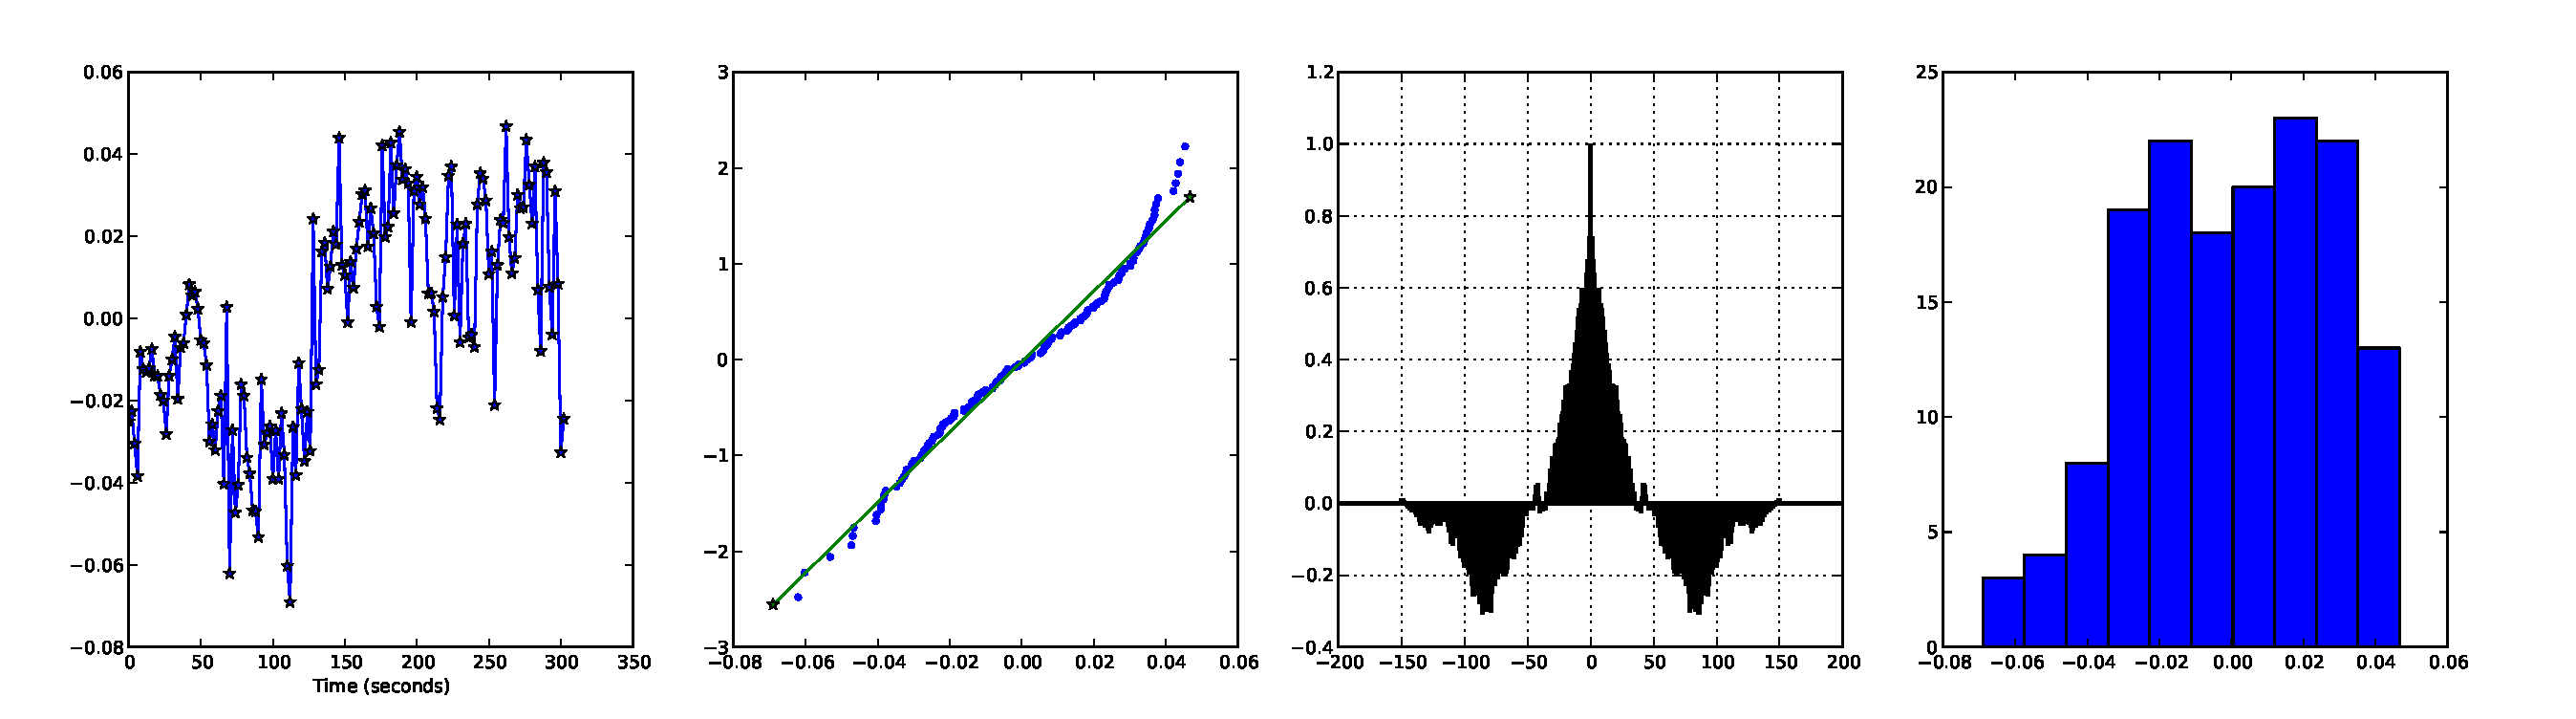
\includegraphics[trim=6cm 1cm 6cm 1cm,width=13cm]{images/noise2_0009_37_29_24}}

%\subfigure{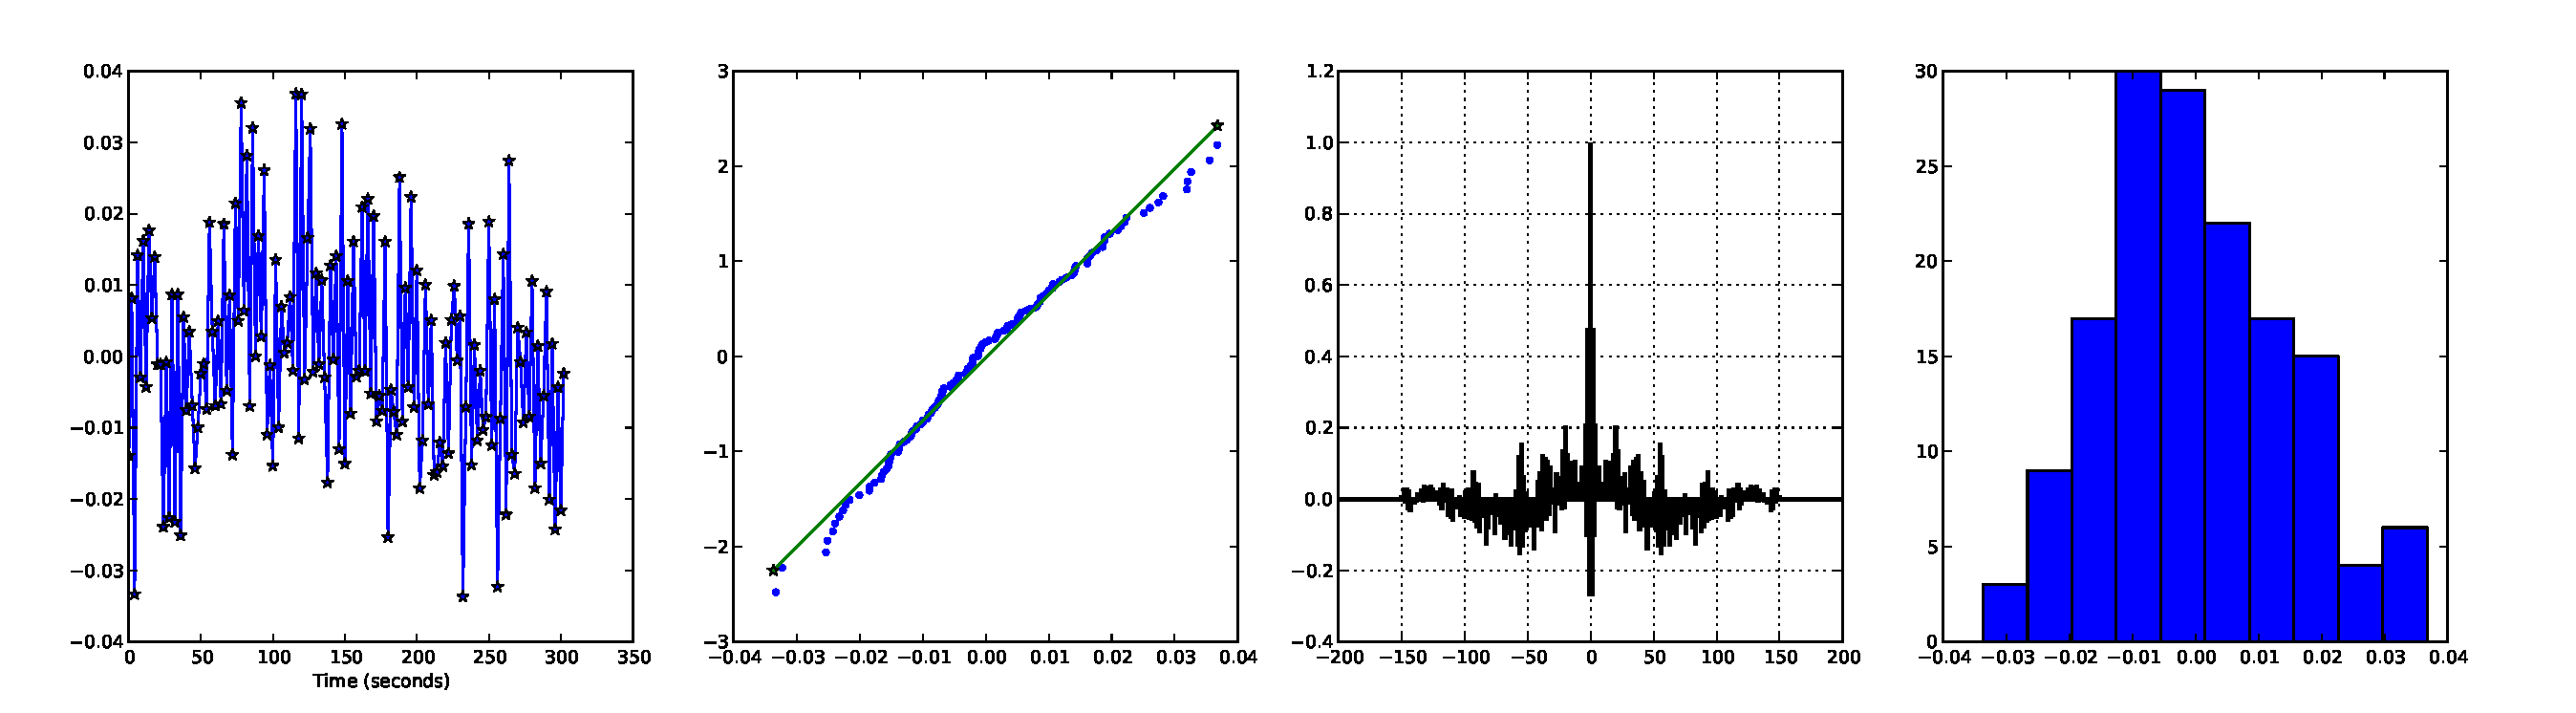
\includegraphics[trim=6cm 1cm 0 0cm,width=17cm]{images/noise_0009_19-24-10.pdf}}
%\subfigure{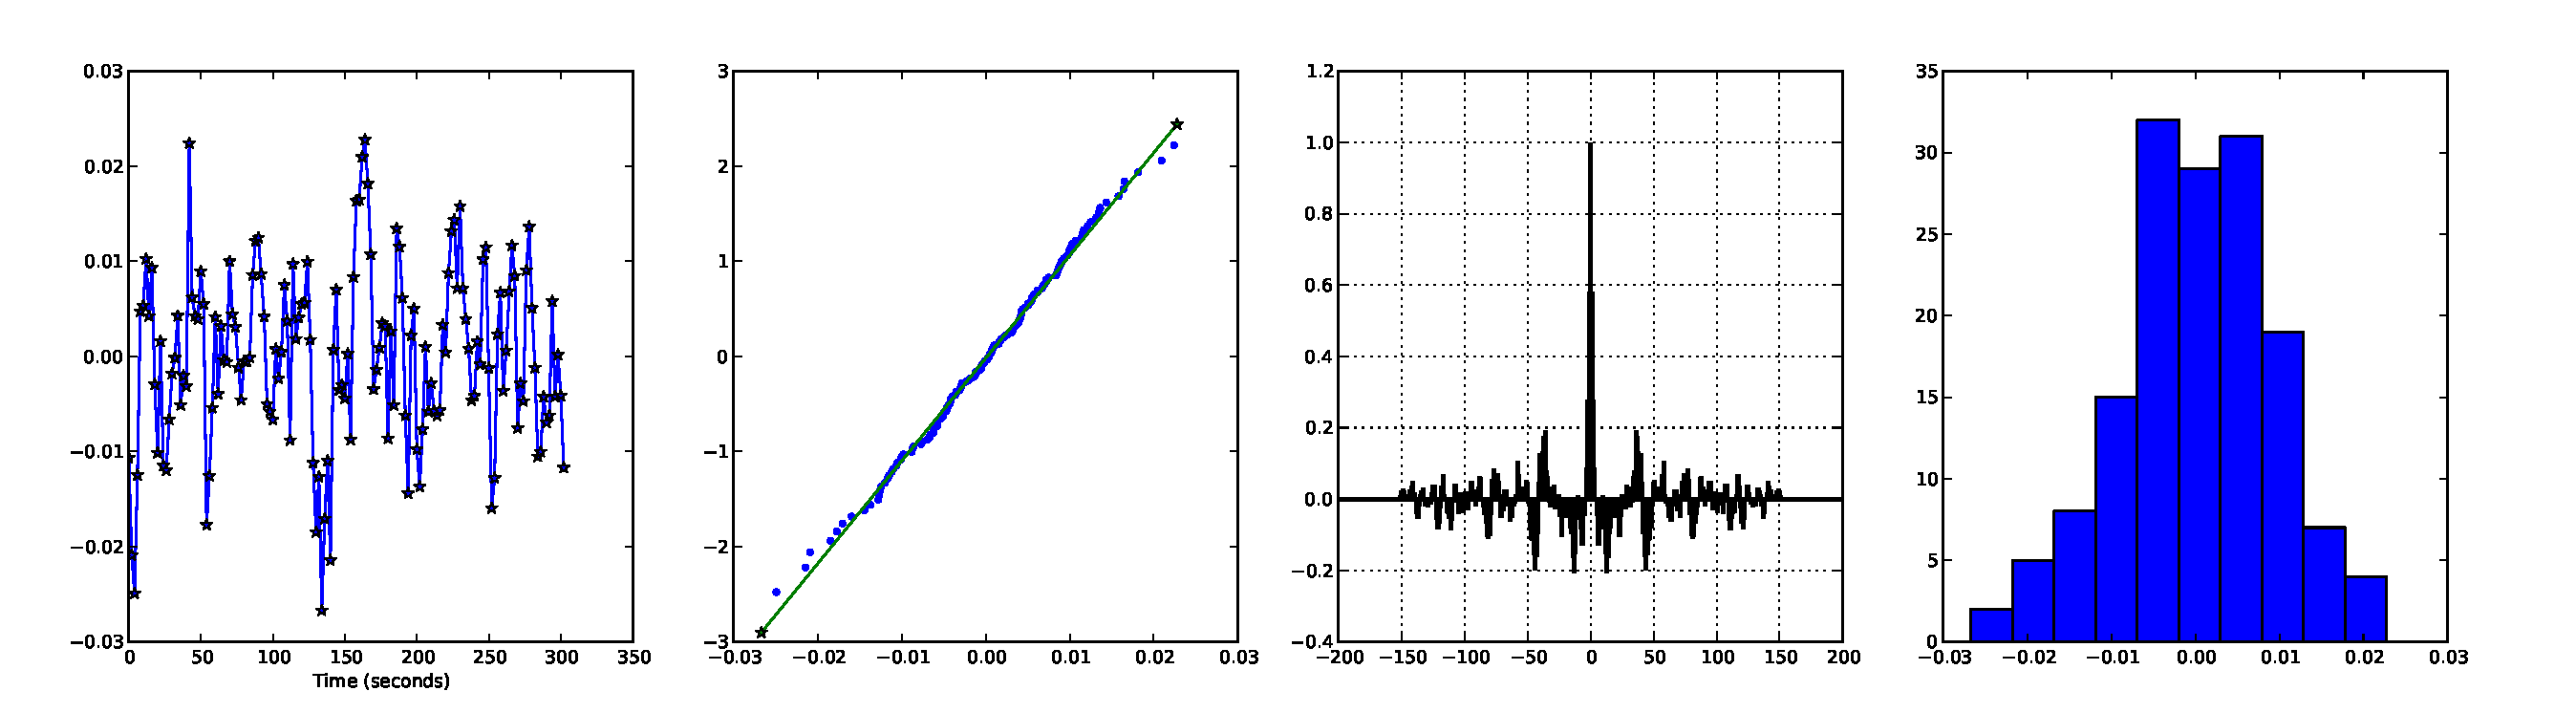
\includegraphics[trim=6cm 1cm 0 0cm,width=17cm]{images/noise_0009_20-45-18.pdf}}
%\subfigure{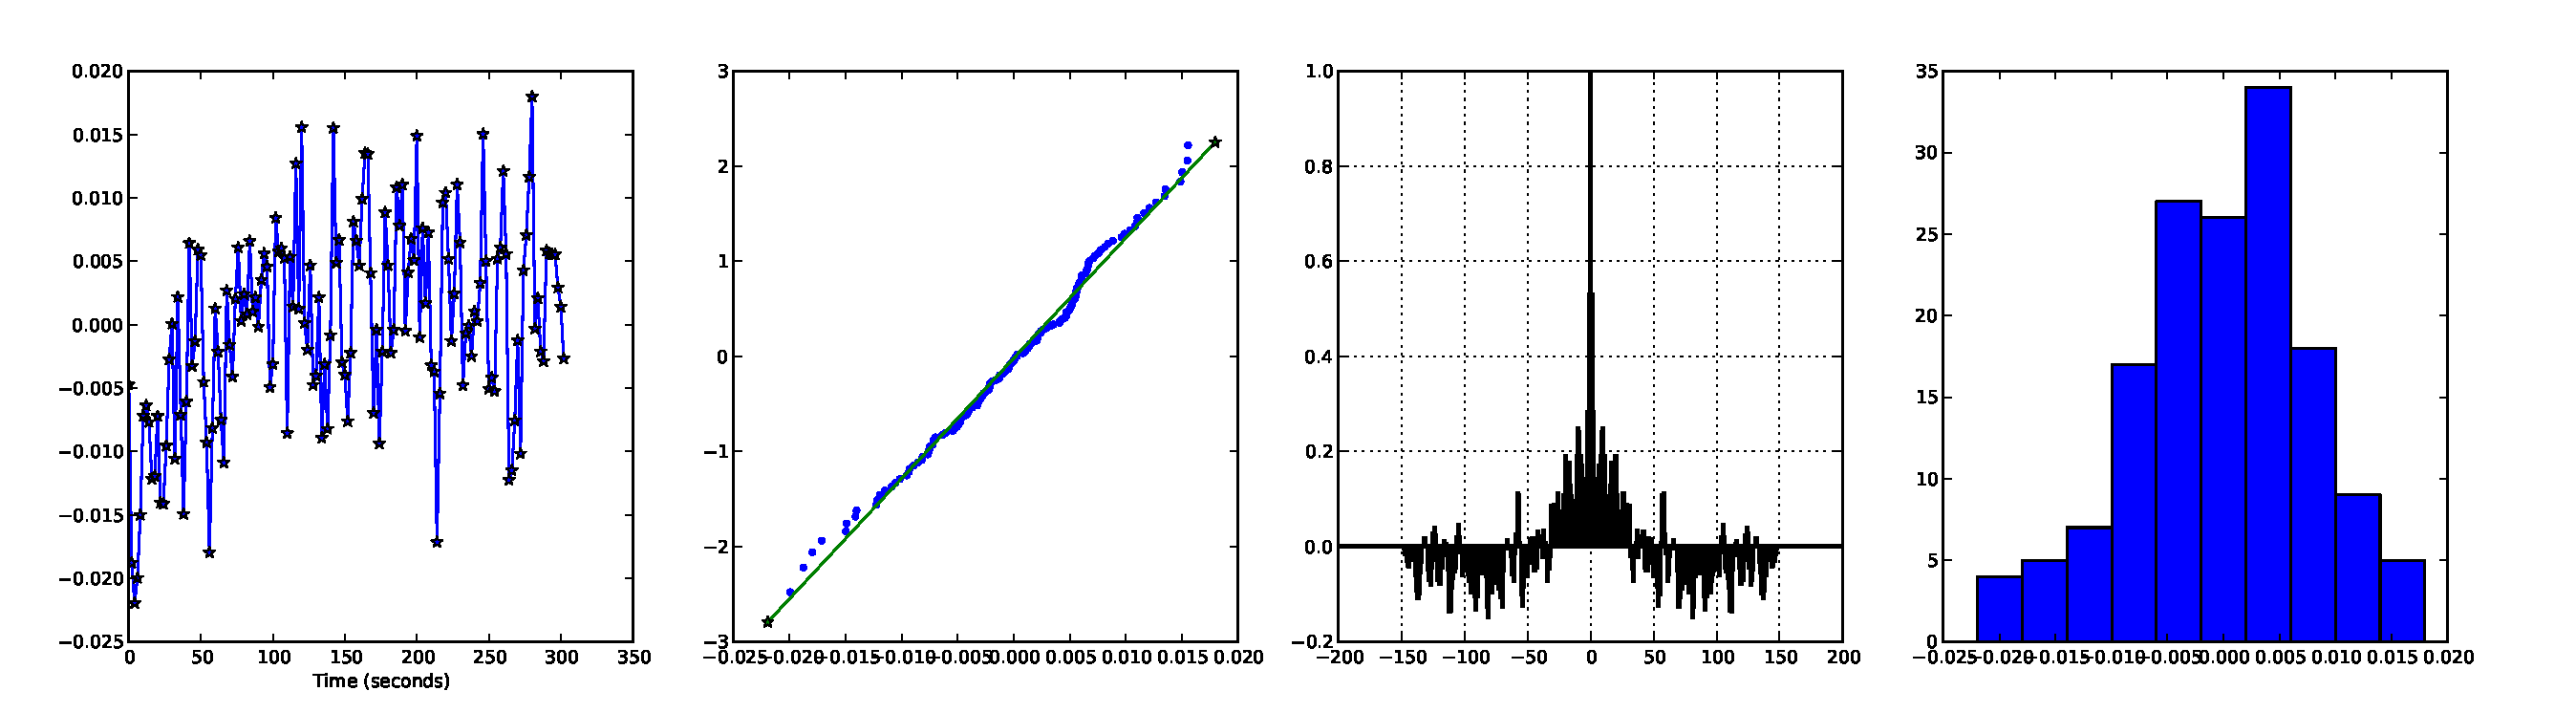
\includegraphics[trim=6cm 1cm 0 0cm,width=17cm]{images/noise_0009_23-47-18.pdf}}
%\subfigure{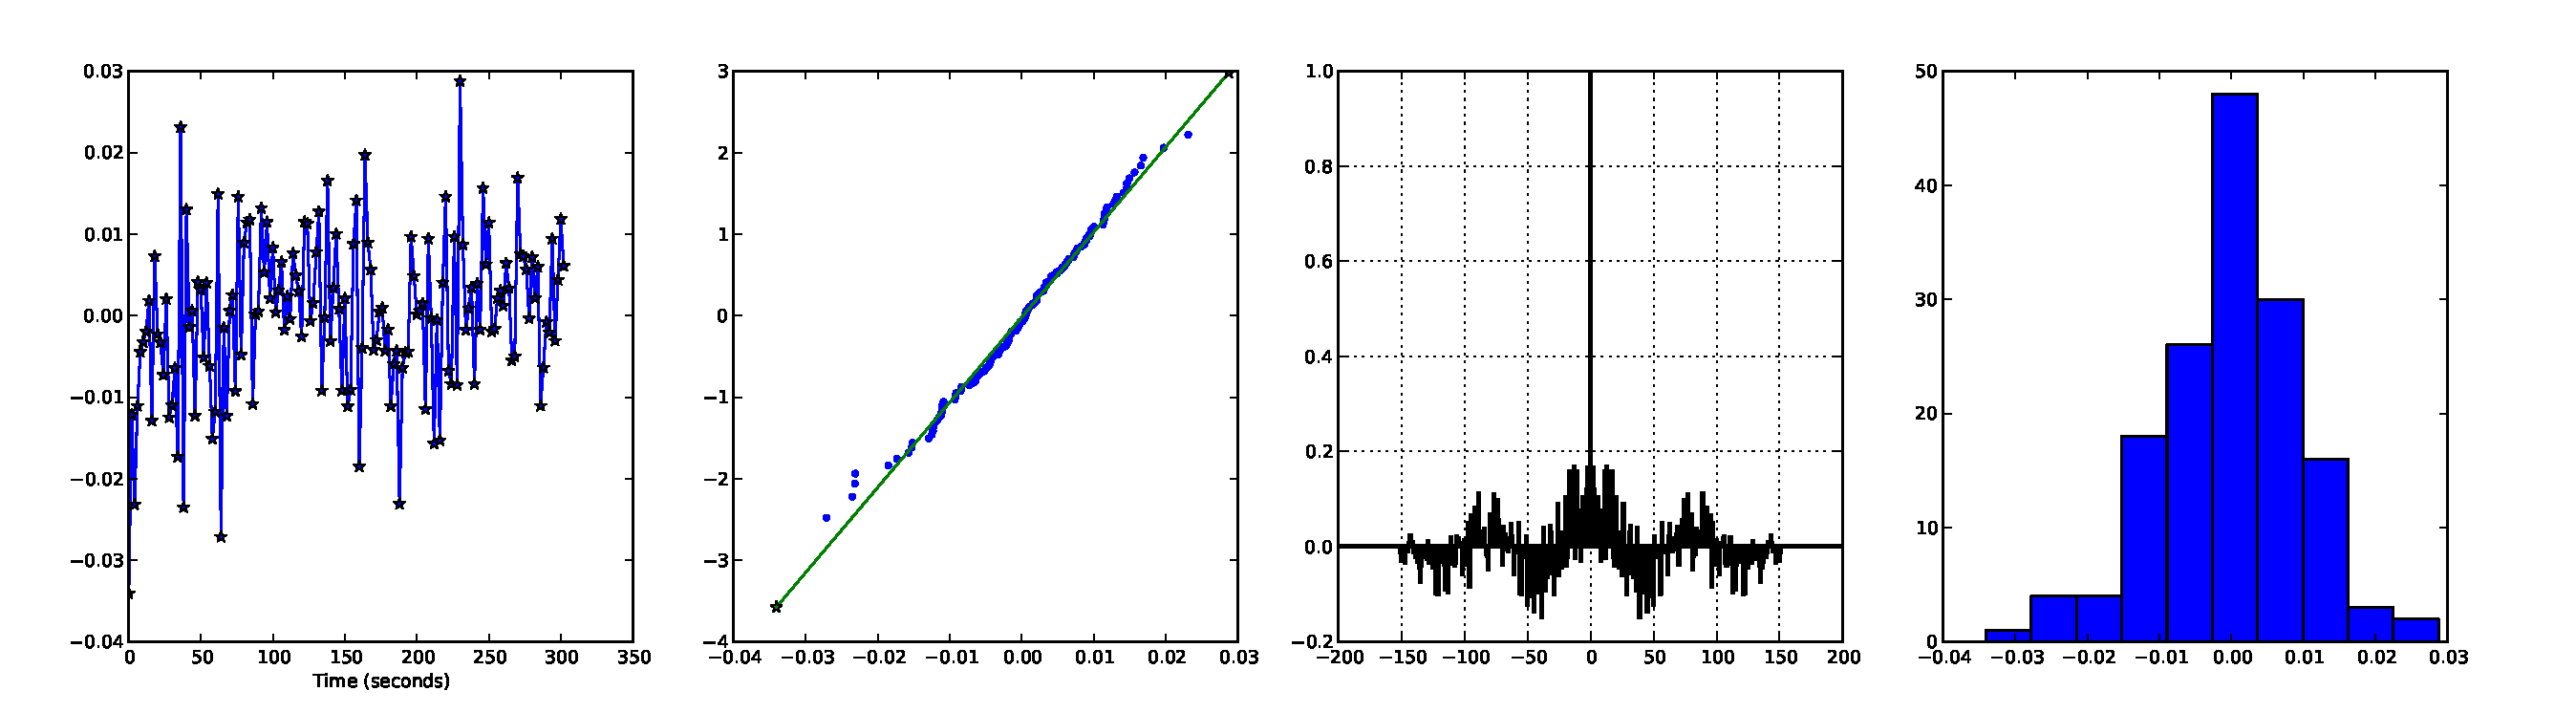
\includegraphics[trim=6cm 1cm 0 0cm,width=17cm]{images/noise_0009_35-49-9.pdf}}

\caption{Q-Q Plots of normalized resting state data}
\label{fig:QQDC}
\end{figure}

\begin{figure}
\centering
\subfigure[]{\label{fig:QQDDelta:A}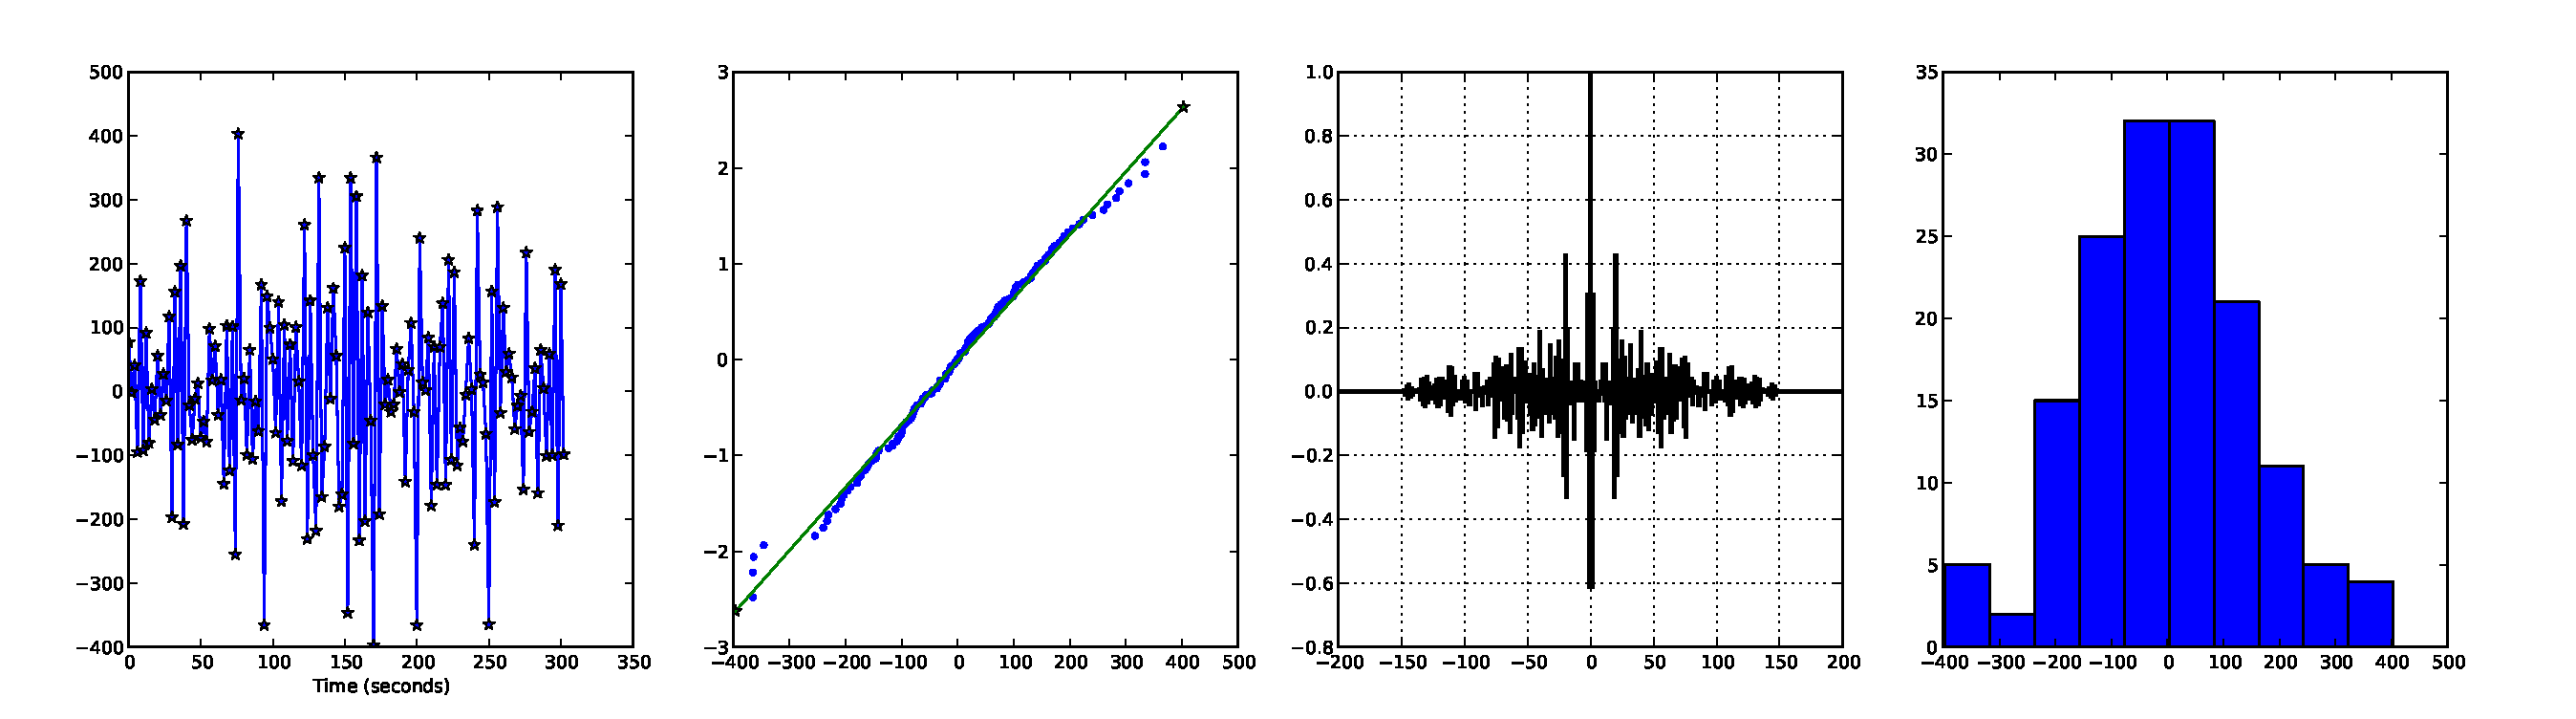
\includegraphics[trim=6cm 1cm 6cm 1cm,width=13cm]{images/noise2_0009d_29_49_9}}
\subfigure[]{\label{fig:QQDDelta:B}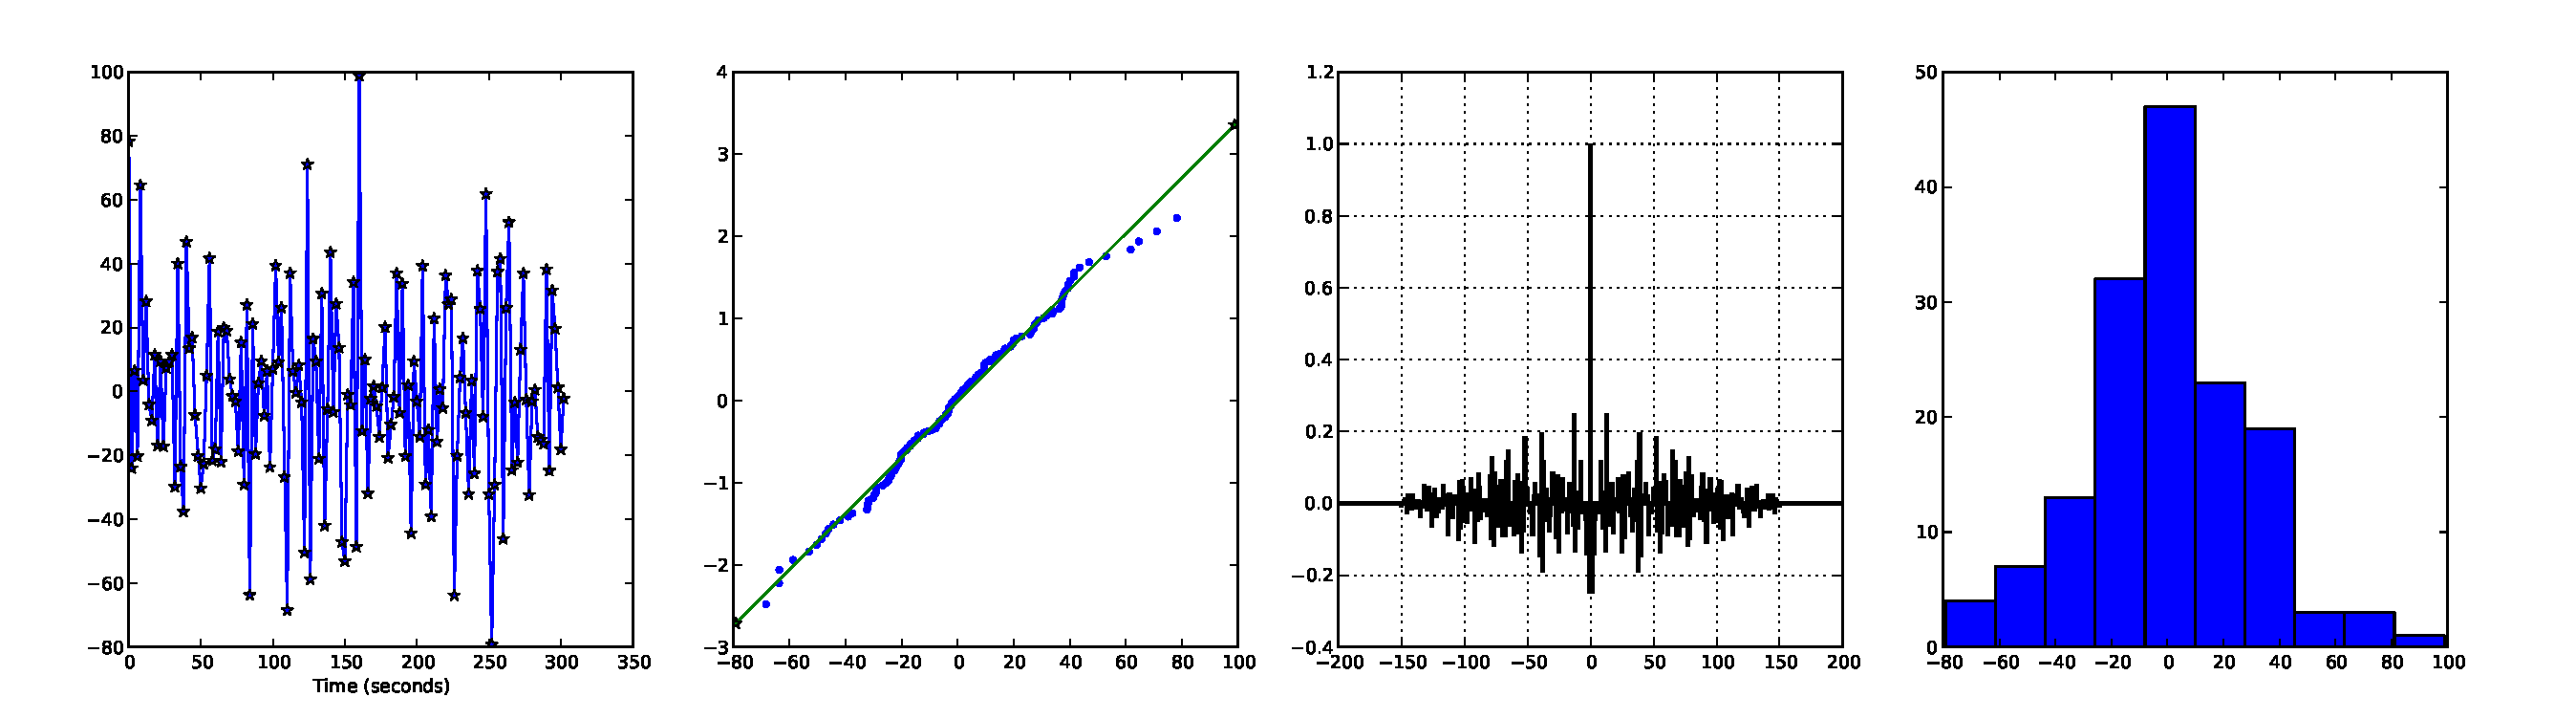
\includegraphics[trim=6cm 1cm 6cm 1cm,width=13cm]{images/noise2_0009d_34_43_24}}
\subfigure[]{\label{fig:QQDDelta:C}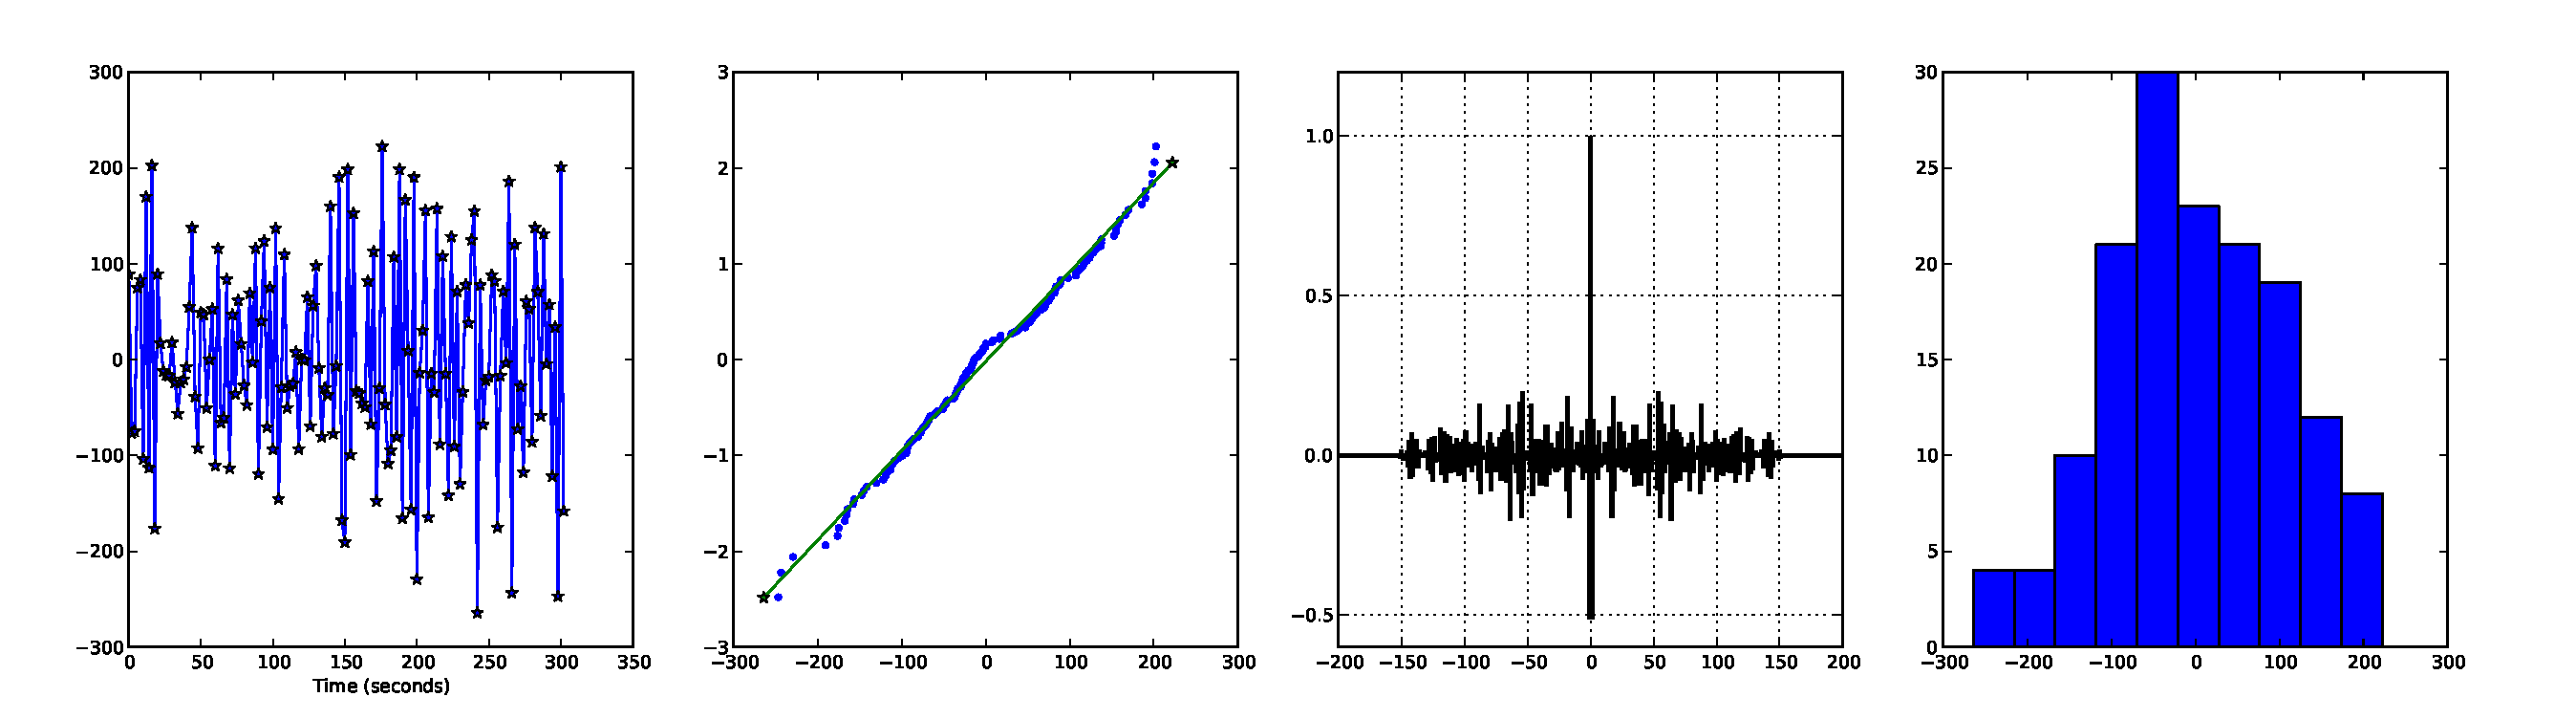
\includegraphics[trim=6cm 1cm 6cm 1cm,width=13cm]{images/noise2_0009d_22_38_23}}
\subfigure[]{\label{fig:QQDDelta:D}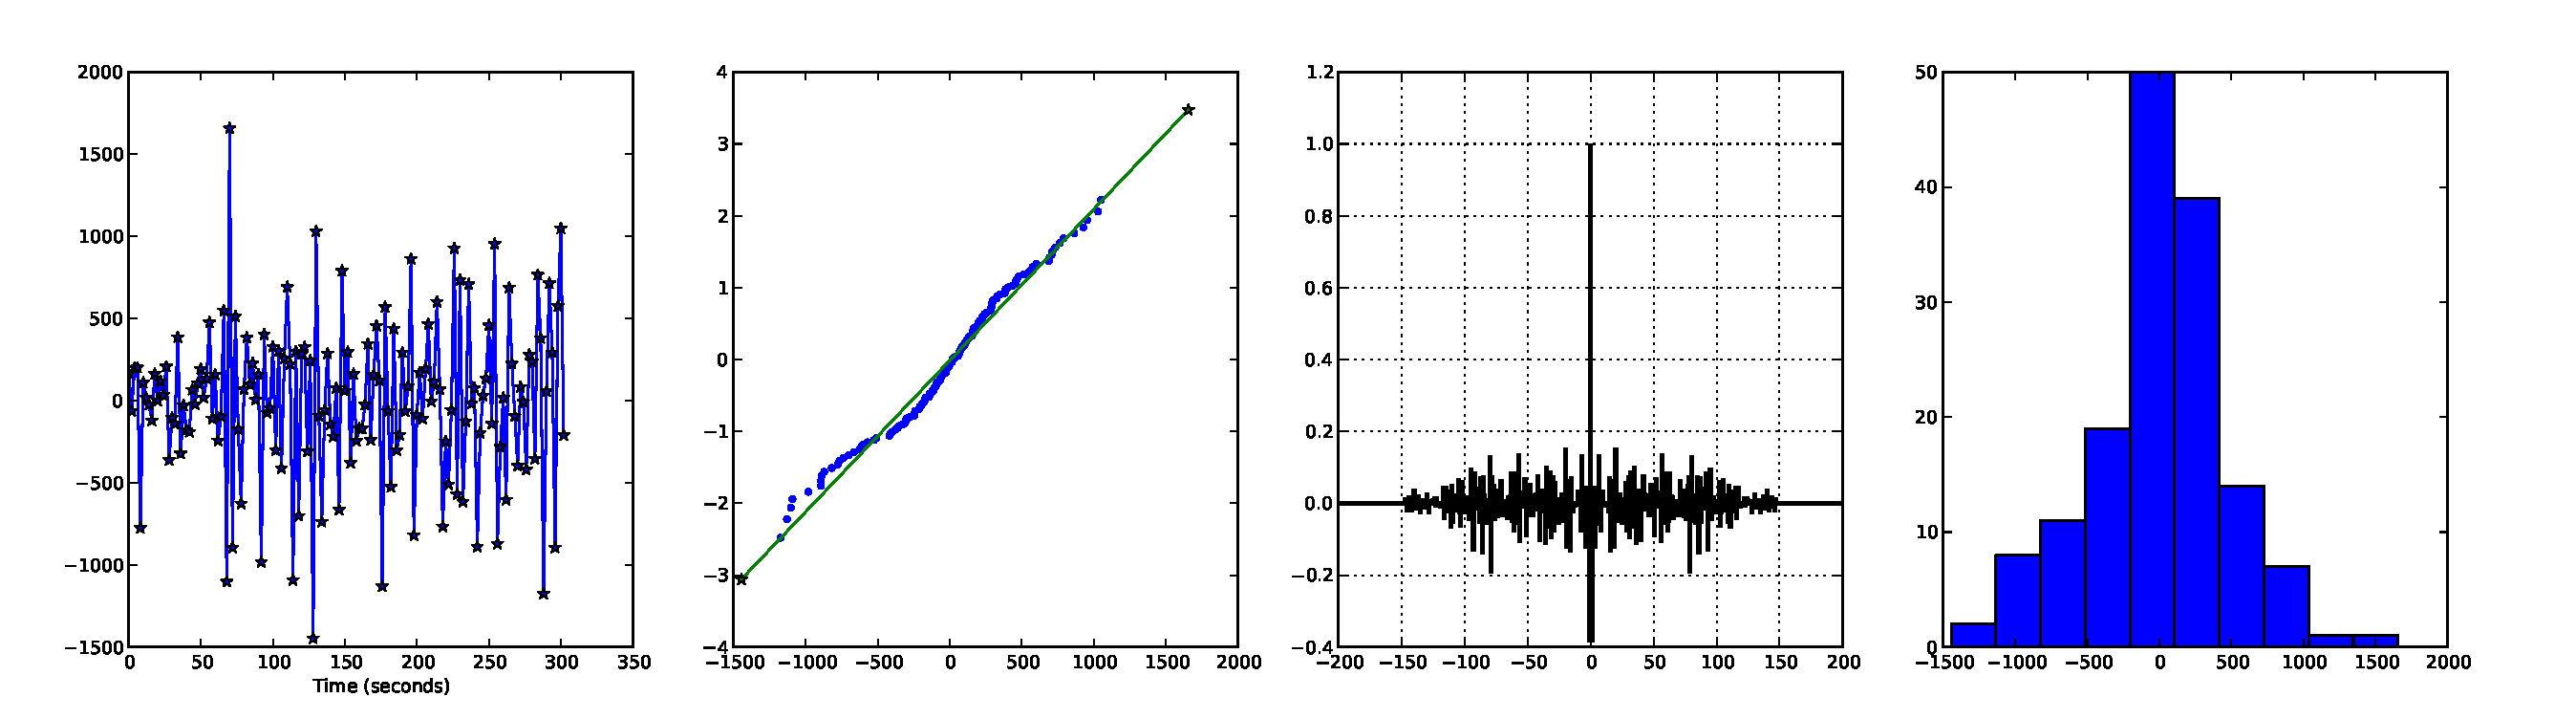
\includegraphics[trim=6cm 1cm 6cm 1cm,width=13cm]{images/noise2_0009d_37_29_24}}
\caption{Q-Q Plots of resting state data, using the BOLD signal changes}
\label{fig:QQDelta}
\end{figure}


\begin{figure}
\centering
\subfigure[]{\label{fig:QQs:A}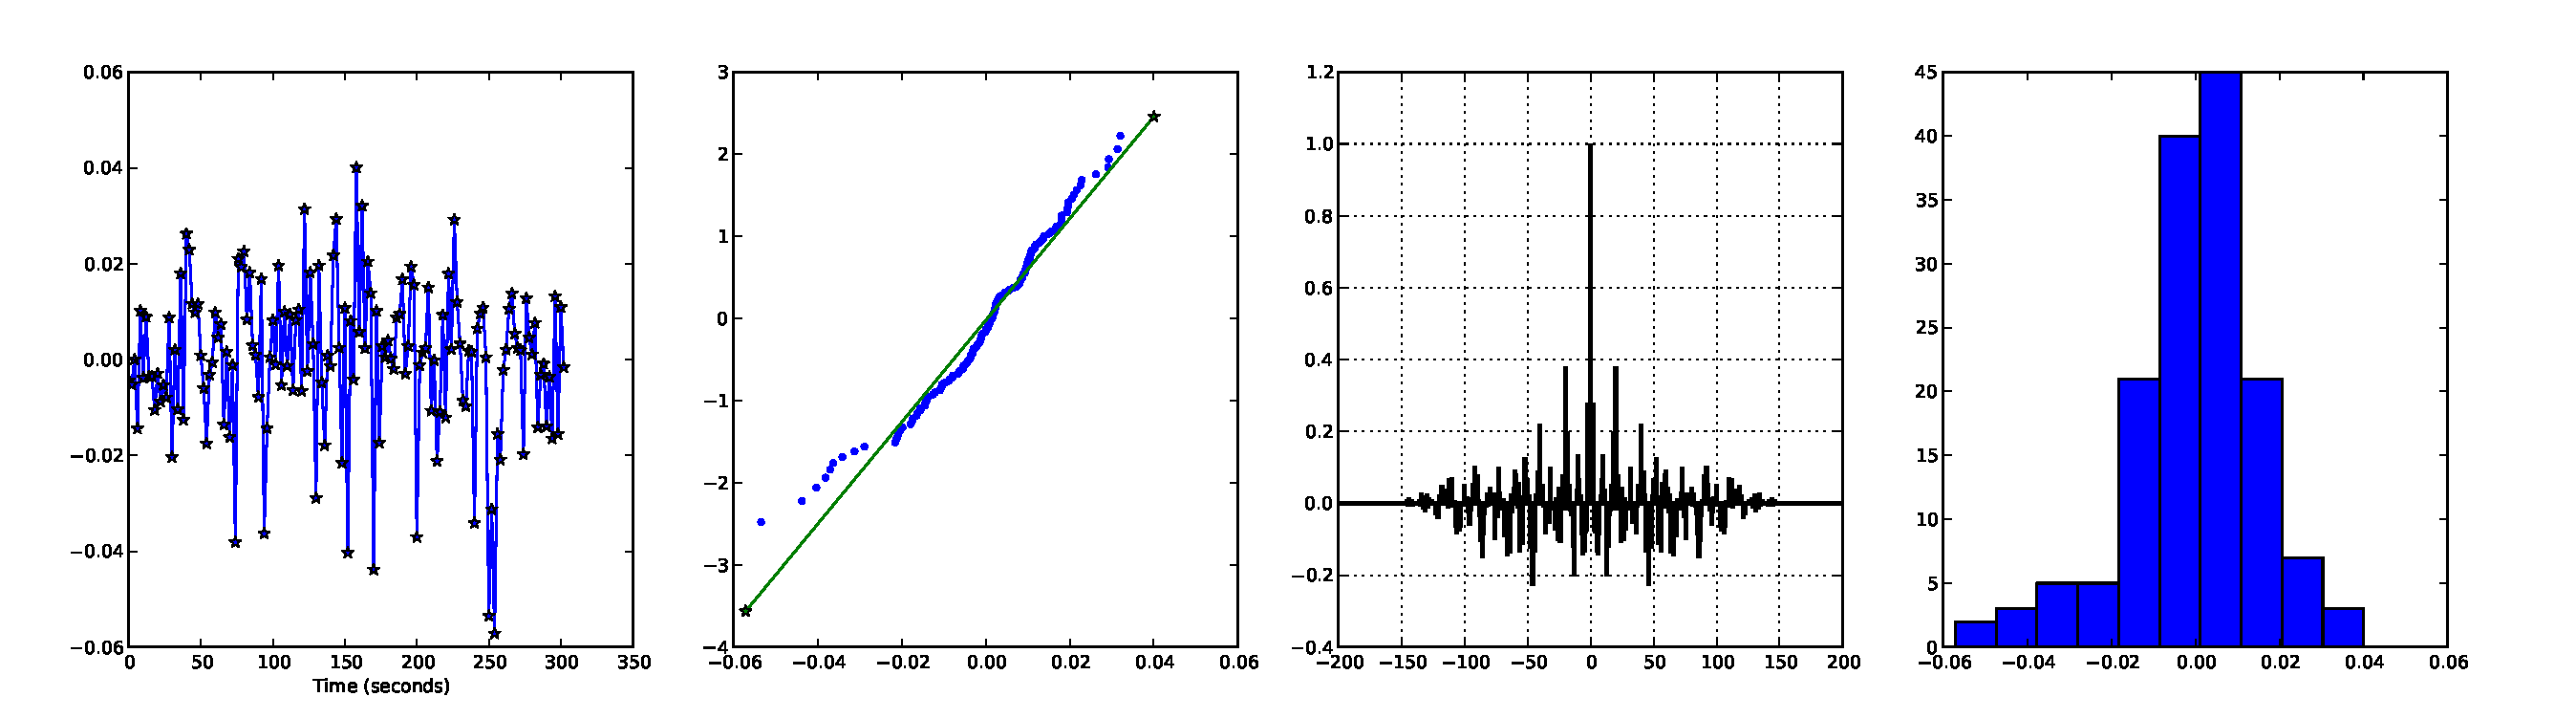
\includegraphics[trim=6cm 1cm 6cm 1cm,width=13cm]{images/noise2_0009s_29_49_9}}
\subfigure[]{\label{fig:QQs:B}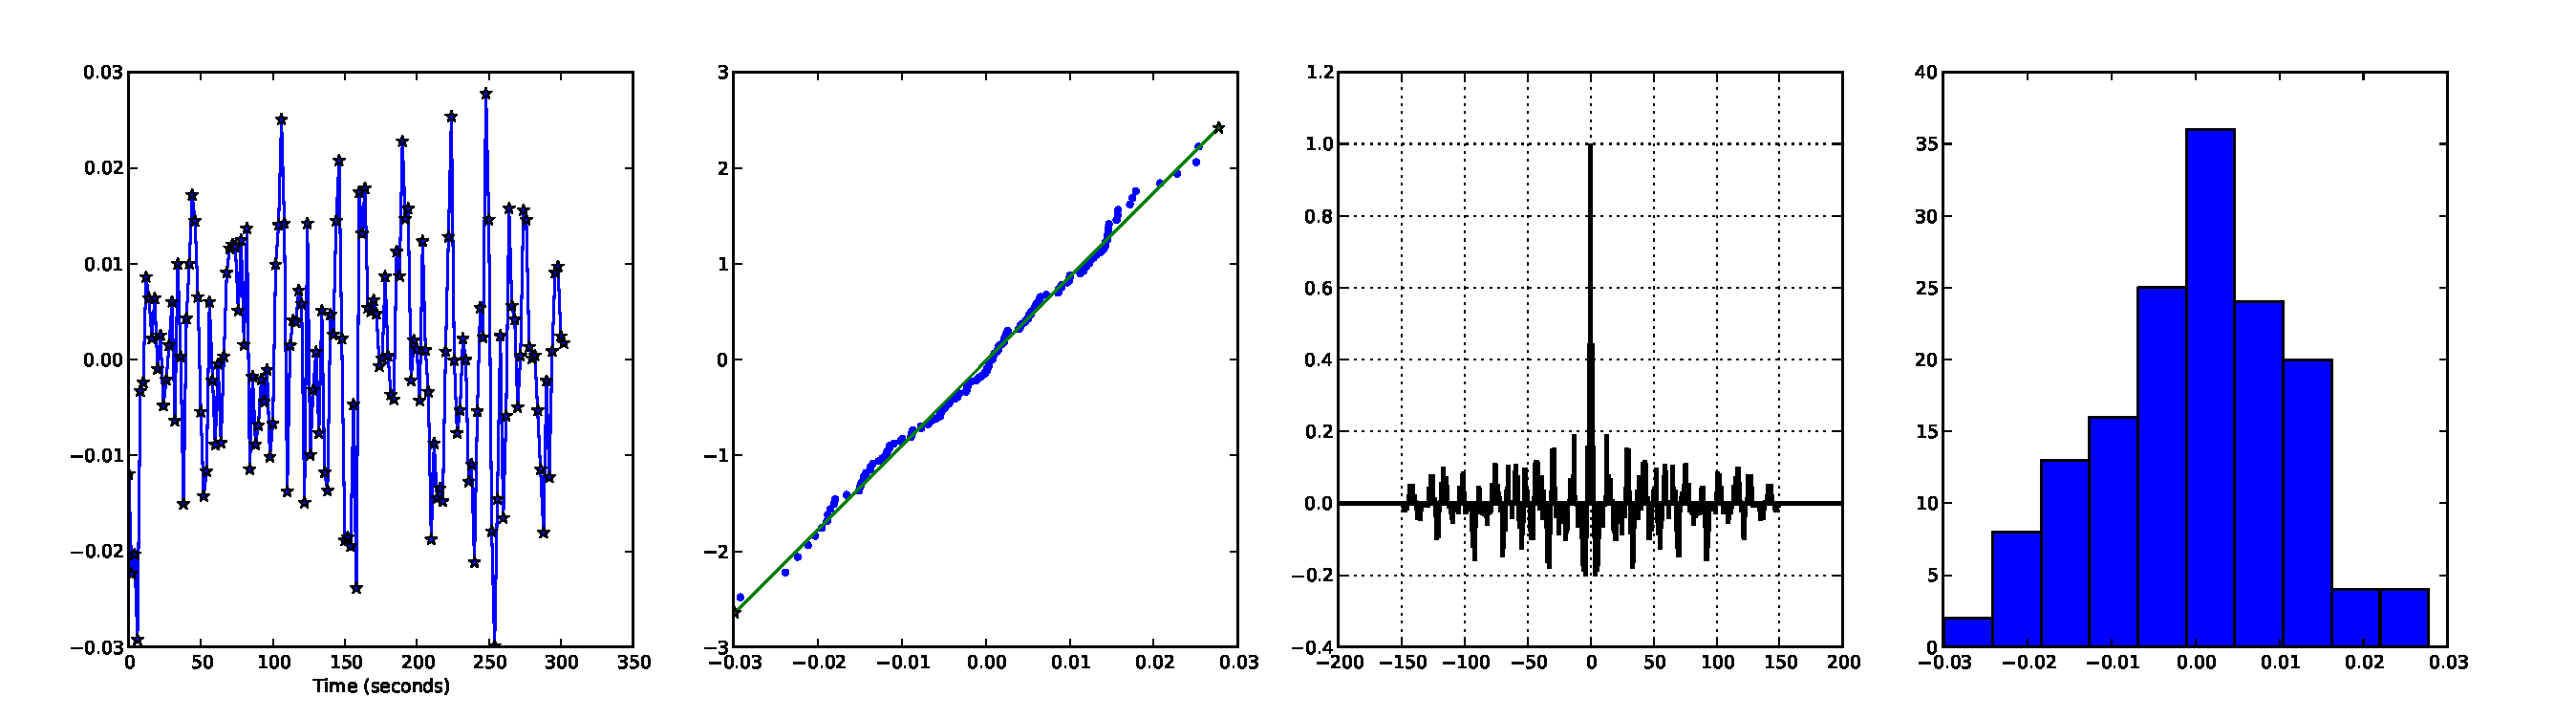
\includegraphics[trim=6cm 1cm 6cm 1cm,width=13cm]{images/noise2_0009s_34_43_24}}
\subfigure[]{\label{fig:QQs:C}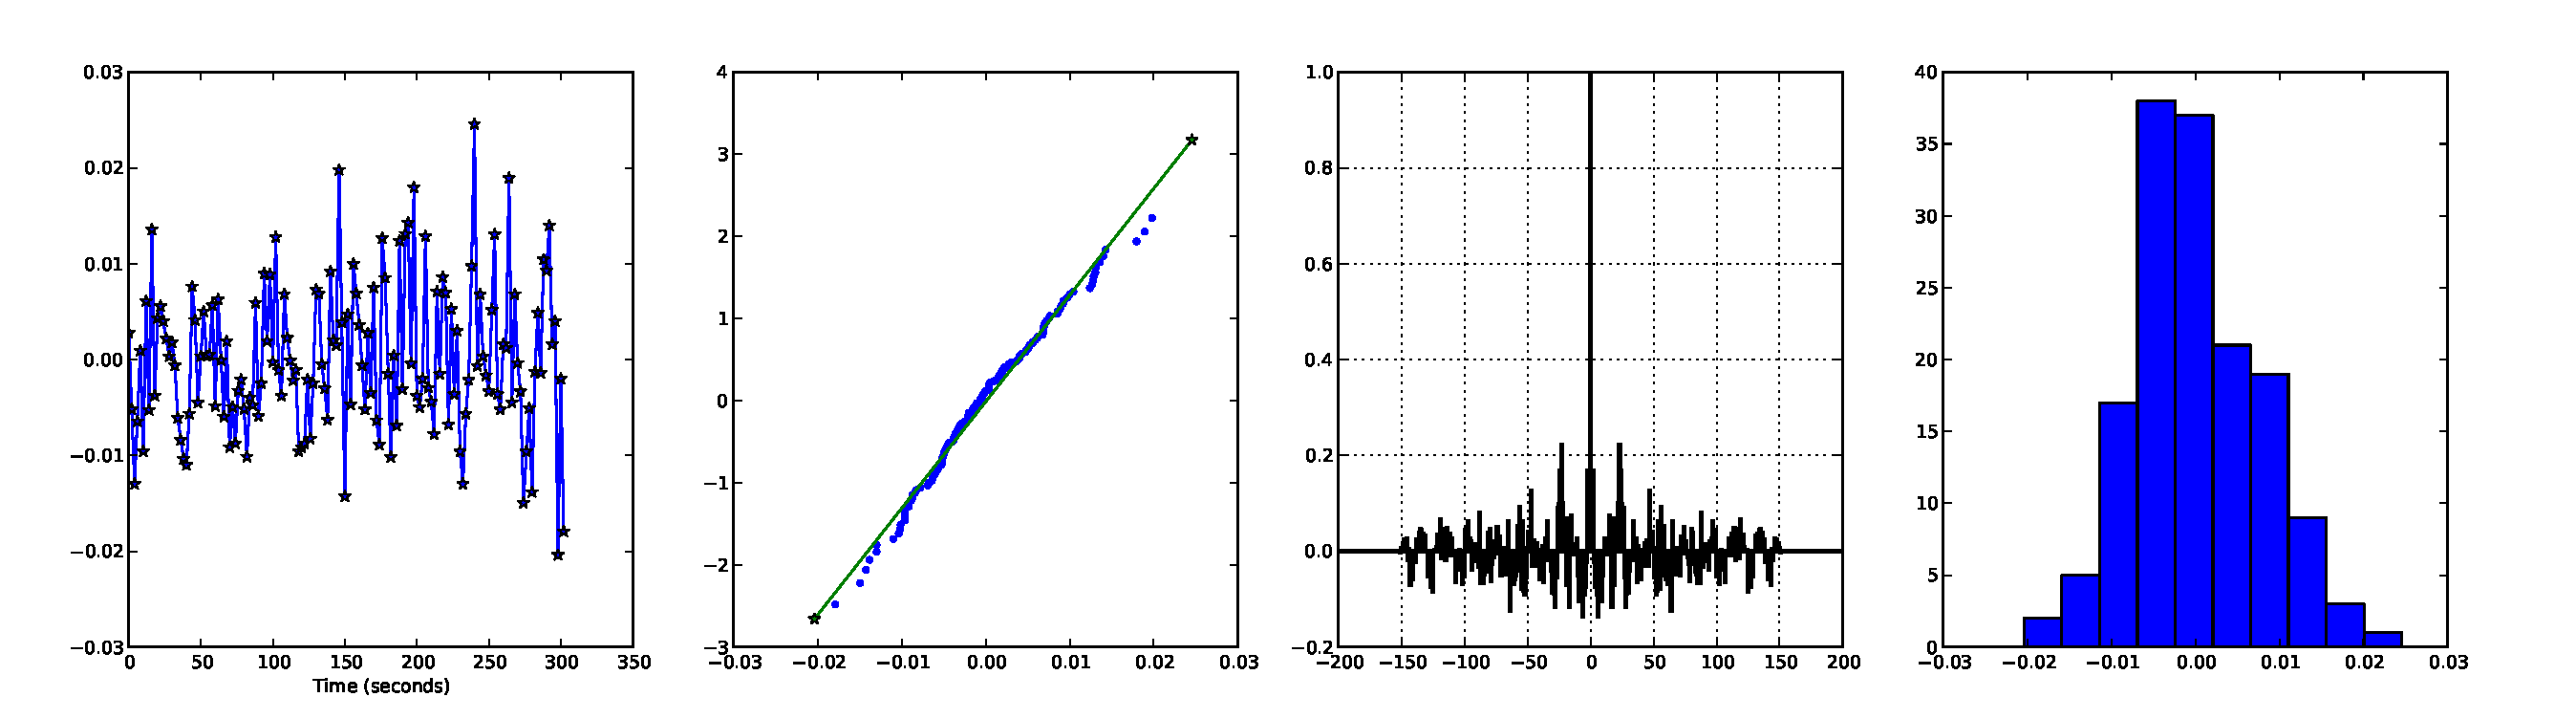
\includegraphics[trim=6cm 1cm 6cm 1cm,width=13cm]{images/noise2_0009s_22_38_23}}
\subfigure[]{\label{fig:QQs:D}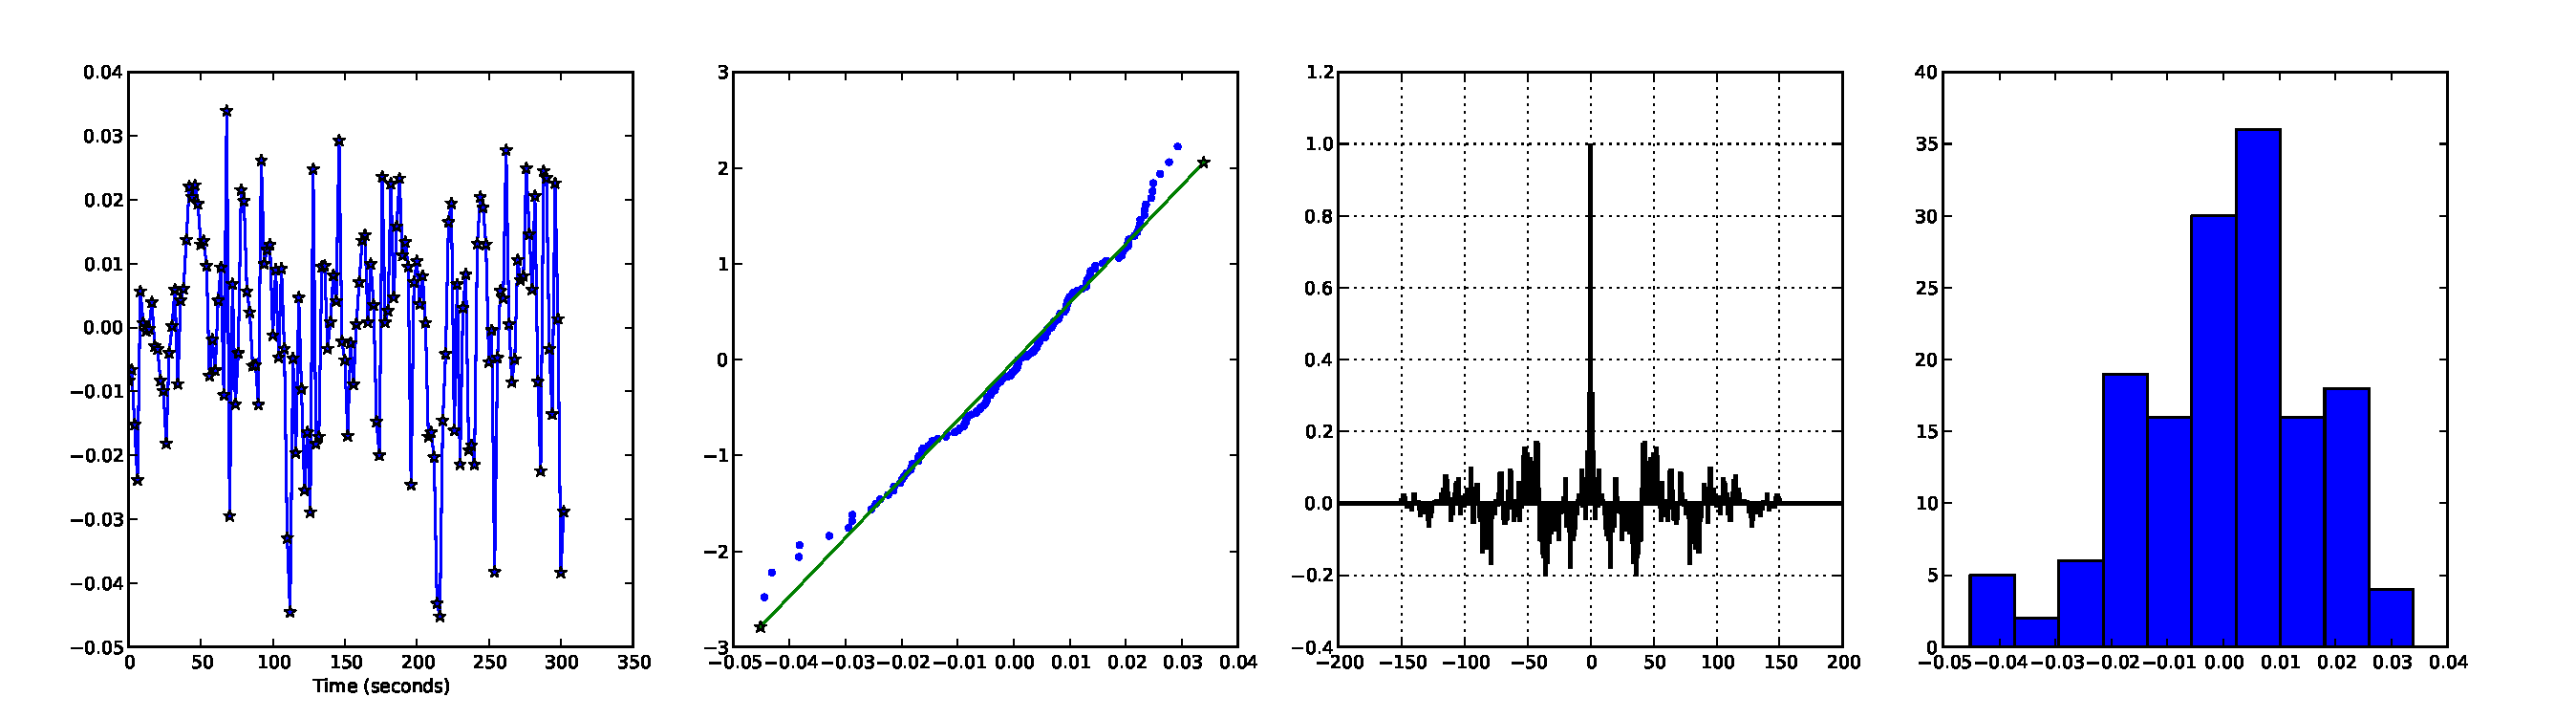
\includegraphics[trim=6cm 1cm 6cm 1cm,width=13cm]{images/noise2_0009s_37_29_24}}
\caption{Q-Q Plots of resting state data, after the de-trending}
\label{fig:QQSpline}
\end{figure}

Because most methods (including the one used in this paper)
assume the noise realizations are independent of each other, the auto-
correlation is of particular interest (which is a necessary but not
sufficient condition for independence). Gaussianity is also a common
assumption made in studies of FMRI data, though that assumption is not
needed in this work. Regardless, comparing the distribution to a Gaussian
is informative, so Q-Q plots are used to compare example data with the
Normal distribution. Additionally, in FMRI data the noise is often considered 
to be Wiener \cite{Riera2003}. Recall that a Wiener random process is
characterized by steps that are Gaussian and independent. The simulations discussed in 
\autoref{sec:Single Voxel Simulation} make use of this, 
by adding a Wiener random process to the overall signal. To determine
whether the noise is in fact Wiener, the distribution of 
the steps were plotted against a Gaussian. 

Finally, removal of the drift is often performed with a high pass filter,
so analyzed the distribution after subtracting of a spline, (see \autoref{sec:Methods Preprocessing}).

\autoref{fig:QQDC} shows the 
results with a regression line fit to the points.
Recall that in a Quartile-Quartile (Q-Q) plot, if the points plotted on the 
x-axis and the points
on the y-axis come from the same type of distribution, then all the points will
be collinear. Differences in the variance will cause the line to have a slope
other than 1, while differences in the expected value will cause the fitted line
to be shifted. In these Q-Q plots, the points are being compared to the standard
Gaussian distribution. Note that in \autoref{fig:QQDC} the points have all been 
normalized (changed to percent difference).

Note that \autoref{fig:QQDC:A} and \autoref{fig:QQDC:B}
are well described by a Gaussian process with a small autocorrelation, 
\autoref{fig:QQDC:C} and \autoref{fig:QQDC:D} are not. In particular the tails of \autoref{fig:QQDC:C}
do not seem to fit the Gaussian well. Also note the significant autocorrelation in
\autoref{fig:QQDC:C} and \autoref{fig:QQDC:D}. As expected, the noise is not strictly
Gaussian white noise.  On the other hand, the steps do conform rather
closely to the normal distribution.
As expected, most of the autocorrelation disappears for the step data. Given
that the steps seem to fit the Normal distribution, the low autocorrelation
indicates that the steps could be Independently Distributed. 
Therefore, the noise does seem to come close to a Wiener process. 

De-trending the time-series by subtracting a spline fit to the distribution
removed much of the autocorrelation present in \autoref{fig:QQDC:C} and \autoref{fig:QQDC:D},
though not perfectly. Though the distributions still do not exactly fit
the Normal, \autoref{fig:QQs:D} is much improved compared to \autoref{fig:QQDC:D}.
In all, the de-trending is effectively removing Wiener noise. 

\subsection{Detrending}
\label{sec:Detrend}
The non-stationary
aspect of a Weiner process, presumably the result of integrating some
$\nu_x$ is difficult to compensate for, and so many methods
have been developed to compensate for it. \cite{Tanabe2002} and \cite{Smith1999} have
demonstrated that this component is prevalent, and may in fact be an inherent  characteristic
of FMRI. It has been reported that in some studies as many as half the voxels 
benefited from detrending (\cite{Smith2007}). In a head to head comparison, 
\cite{Tanabe2002}, showed that in most cases subtracting off
a spline worked the best. The benefit of the spline versus wavelets, high pass 
filtering or other DC removal techniques is that the frequency response is not set.
Rather, the spline is adaptive to the input. Unfortunately no method will 
perfectly remove noise, and no method will leave the signal untouched.

The method I used to calculate the spline was picking one knot for every 20
measurements in an image. Thus a 10 minute session at a repetition time of 
2.1 seconds would have 19 knots. The knot first and last knots were each 
given half the number of samples as the rest of the knots; which were all 
located at the center of their sample group. The median of each sample group
was then taken and used as the magnitude for the group. Taking the median 
versus the mean seemed to work better, given the presence of outliers. 
There is potential to optimize the spline further using a canonical 
HRF to find resting points; however, for this to work the experiment would have
to be designed with this in mind. 

Problematically, after removing the DC component of the signal,
by definition the signal will have a median near zero. 
Unfortunately this is not the natural state of the BOLD signal. More specifically,
when the signal is inactive, the BOLD response should be at 0\% change from
the base level; activation may then increase, or for short periods decrease from this base.
Because most of the BOLD signal is above baseline, after removing the spline
the BOLD resting state will be below 0\%.  This reduces the ability of an algorithm to learn.
One method of accounting for this is to simply add a DC gain model parameter.
Like all the other model parameters, with enough measurements, a viable
parameter would fall. Yet adding another dimension increases the
complexity of the model, when the parameter is relatively easy to estimate
by visual inspection.  In this work a simpler approach was used. To determine
the DC gain I used a robust estimator of scale. The Median Absolute Deviation (MAD)
proved to be accurate in determining how much to shift the signal up
by. I tested both methods during the course of analysis, and found that the increase 
in model complexity far outweighed the slight increase in flexibility. Other
methods may work better, however the MAD worked well, 
as \autoref{fig:PreprocessedLowNoise} and \autoref{fig:PreprocessedHighNoise} show. 

\begin{equation}
y_{\text{gain}, 0:K} = 1.4826\text{median}_{i=0:K}(y_i - \text{median}(y_{0:K}))
\end{equation}

A serious concern when adding and subtracting arbitrary values to 
real data is whether this will create false positives. This is a legitimate
concern; however, a boosted response does not effect how well the BOLD model 
predicts the actual measurements. 

%\subsection{Linearizing Noise}
%\label{sec:Methods Delta Based Inference}
%The alternative to these sorts of low frequency manipulation is to
%go around the problem in another way. Here, I propose a 
%different method of dealing with the drift. 
%Instead of comparing the direct output of the particle filter with the direct
%measurement, the algorithm would compare the change in signal over a single TR,
%with the result of integrating the model for the same period. 
%In most signal processing cases this would be foolish, but that is because the 
%general assumption is that all noise is high frequency. Considering 
%the fact that every BOLD analysis pipeline uses a high pass filter,
%whereas low poss temporal filter are rarely applied, it makes sense
%that a derivative type method could work. The benefit of particle filters
%is that they are a robust method of inference, and I would assert 
%that the particle filter ought to be given as \emph{raw} data as possible. 
%While taking direct measurements
%without de-trending would give awful results, using the difference removes the 
%DC component and turns what is usually assumed to be a Weiner process into 
%a simple Gaussian random variable. 
%
%\begin{equation}
%\Delta y = y(t) - y(t-1) = g(x(t)) - g(x(t-1)) + \nu_y(t) - \nu_y(t-1) + \nu_d(t) - \nu(t-1)
%\label{eq:measass_delta}
%\end{equation}
%
%Even if $\nu_d$ is some other additive process, the difference will still be closer
%to I.I.D. than a Wiener process, as the autocorrelation of the $\delta y$ shows
%in \autoref{fig:QQDelta} in \autoref{sec:Introduction Noise}. 
% All the assumptions made originally
%for the particle filter still hold, and all of the parameters may be distinguished based on
%the step sizes, thus it is not unreasonable to consider matching the string of step sizes
%rather than string of direct readings. 
%
%\begin{figure}
%\label{fig:FrequencyGraphs}
%\caption{frequency response graphs, highlighting noise frequency range and signal frequency range}
%\end{figure}

\section{Particle Filter Settings}
There are quite a few options when using a particle filter; those
options will be discussed in this section.

\section{Prior Distribution}
\label{sec:PriorDist}
For the BOLD model described in \autoref{sec:BOLD Physiology}, several
different studies have endeavored to calculate parameters. The results
of these studies may be found in \autoref{tab:Params}, and the methods 
used for each may be found in \autoref{sec:Prior Works}. Unfortunately,
\cite{Friston2000} only studied regions deemed active by the General 
Linear Model; and most other research (including \cite{Friston2001}) used these results as 
the source for their priors. 
The one exception is \cite{Johnston2008}, which came to a extremely different
distributions. For a particle filter, the choice of a prior is
the single most important design choice. A very wide prior will require
more particles to be sufficiently dense, a very thin (low variance) prior may miss
the true parameters. Consequently, for this work it was natural
to use priors that will give results consistent with previous works, 
\cite{Friston2000}. This constrains the usefulness of the model to
areas that fall within the prior distribution, yet will allow results
to be comparable to other works. There is a significant need for better
estimates of the physiological parameters; and, while physical experiments
may not be possible, it would not be unreasonable to do a study with
exhaustive simulated annealing or hill climbing tests for multiple
regions and multiple patients.

There is an interesting anomaly with the priors found in virtually all
the works that characterized the parameters, except \cite{Johnston2008}.
The BOLD signal is universally recognized to be around $2-3\%$, maybe
reaching $5\%$ in extreme activation. Yet using the mean priors
from \cite{Friston2000}, the signal response for a $.1$ second
impulse only reaches maybe half a percent, as \autoref{fig:MeanResponseF}
shows.

\begin{figure}
\centering
\label{fig:MeanResponseF}
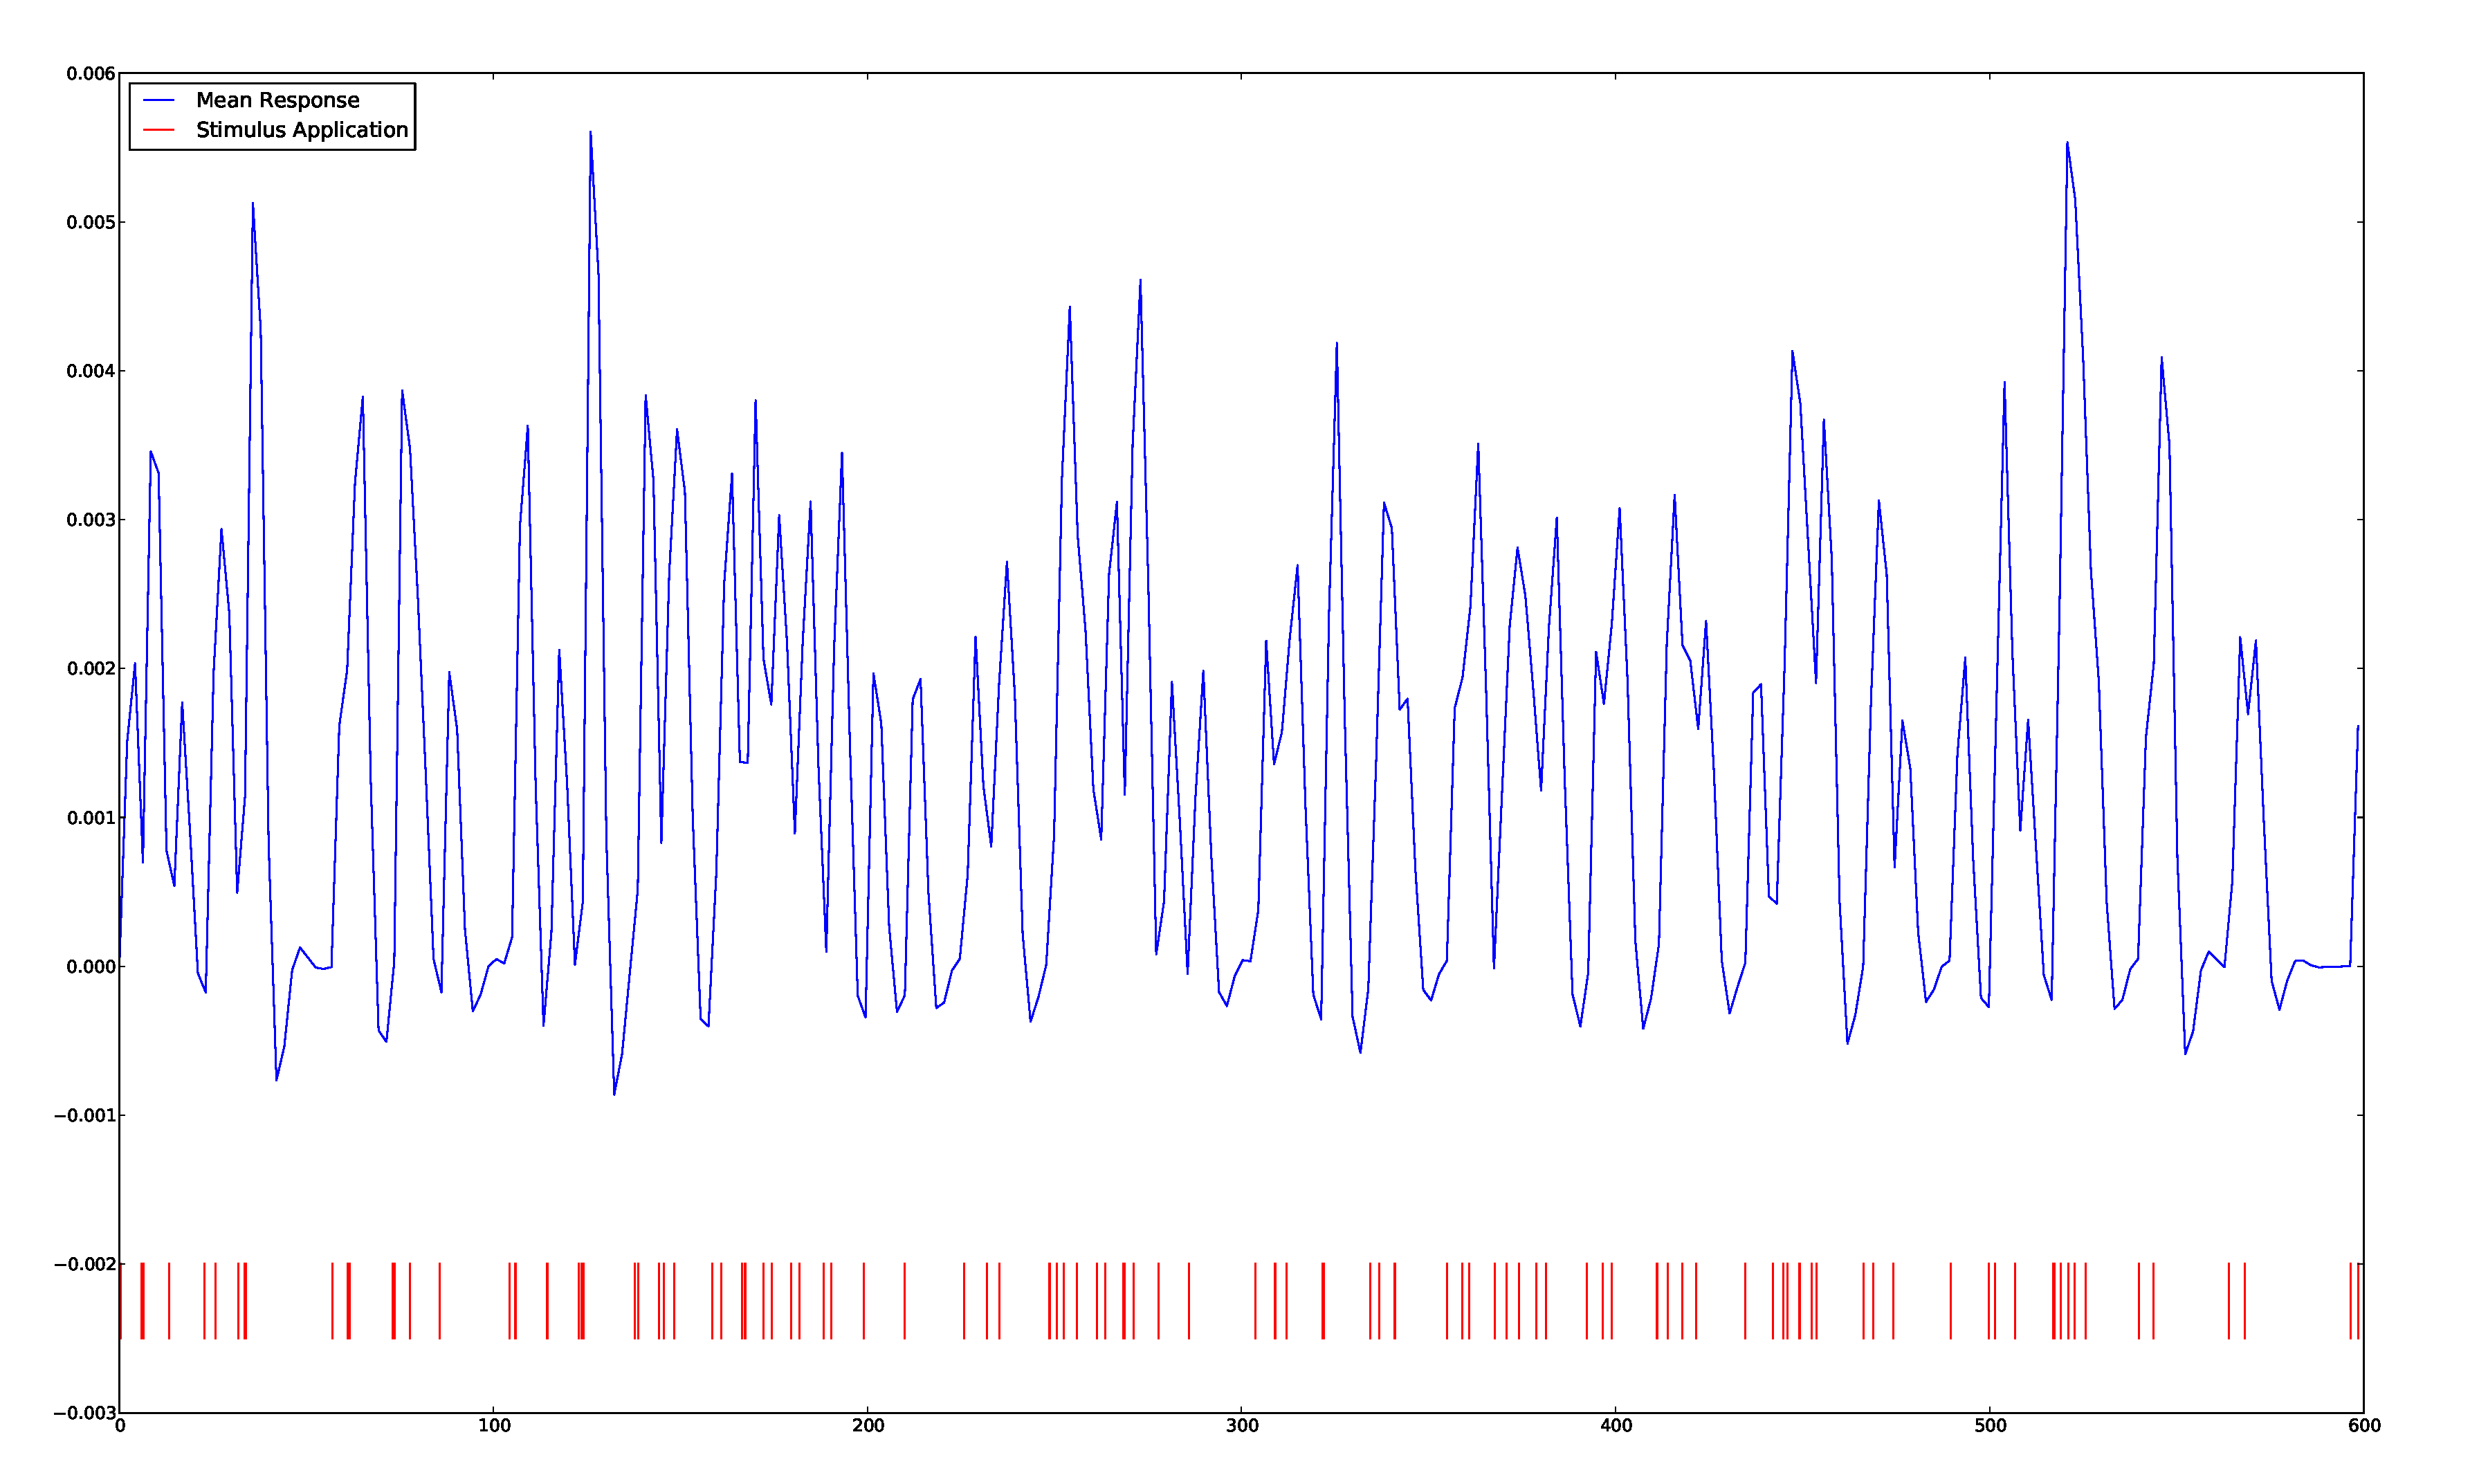
\includegraphics[trim=6cm 3cm 6cm 3cm,width=16cm]{images/mean_response}
\caption{Response to $.1s$ impulses with the mean parameters from \cite{Friston2000}}
\end{figure}

While this could be the result of a stimulus
being too short to lead to strong activation, a similar stimulus
scheme in real data showed a much larger response than 
half a percent as well. In fact, after applying de-trending,
converting the image to percent-difference, and removing 
outliers ($ BOLD > 10\% \text{ or } BOLD < -10\%$) the total variance
across all \emph{active} voxels was still around .02, indicating
that in active voxels a signal peaking below .005 seems unlikely. 
Of course, if more restriction were placed on the outliers, its possible
this standard deviations could be brought down. 
The parameter estimates by \cite{Johnston2008} are even more 
confusing, with peaks of well below $.1\%$ (\autoref{fig:MeanResponseJ}).

\begin{figure}
\centering
\label{fig:MeanResponseJ}
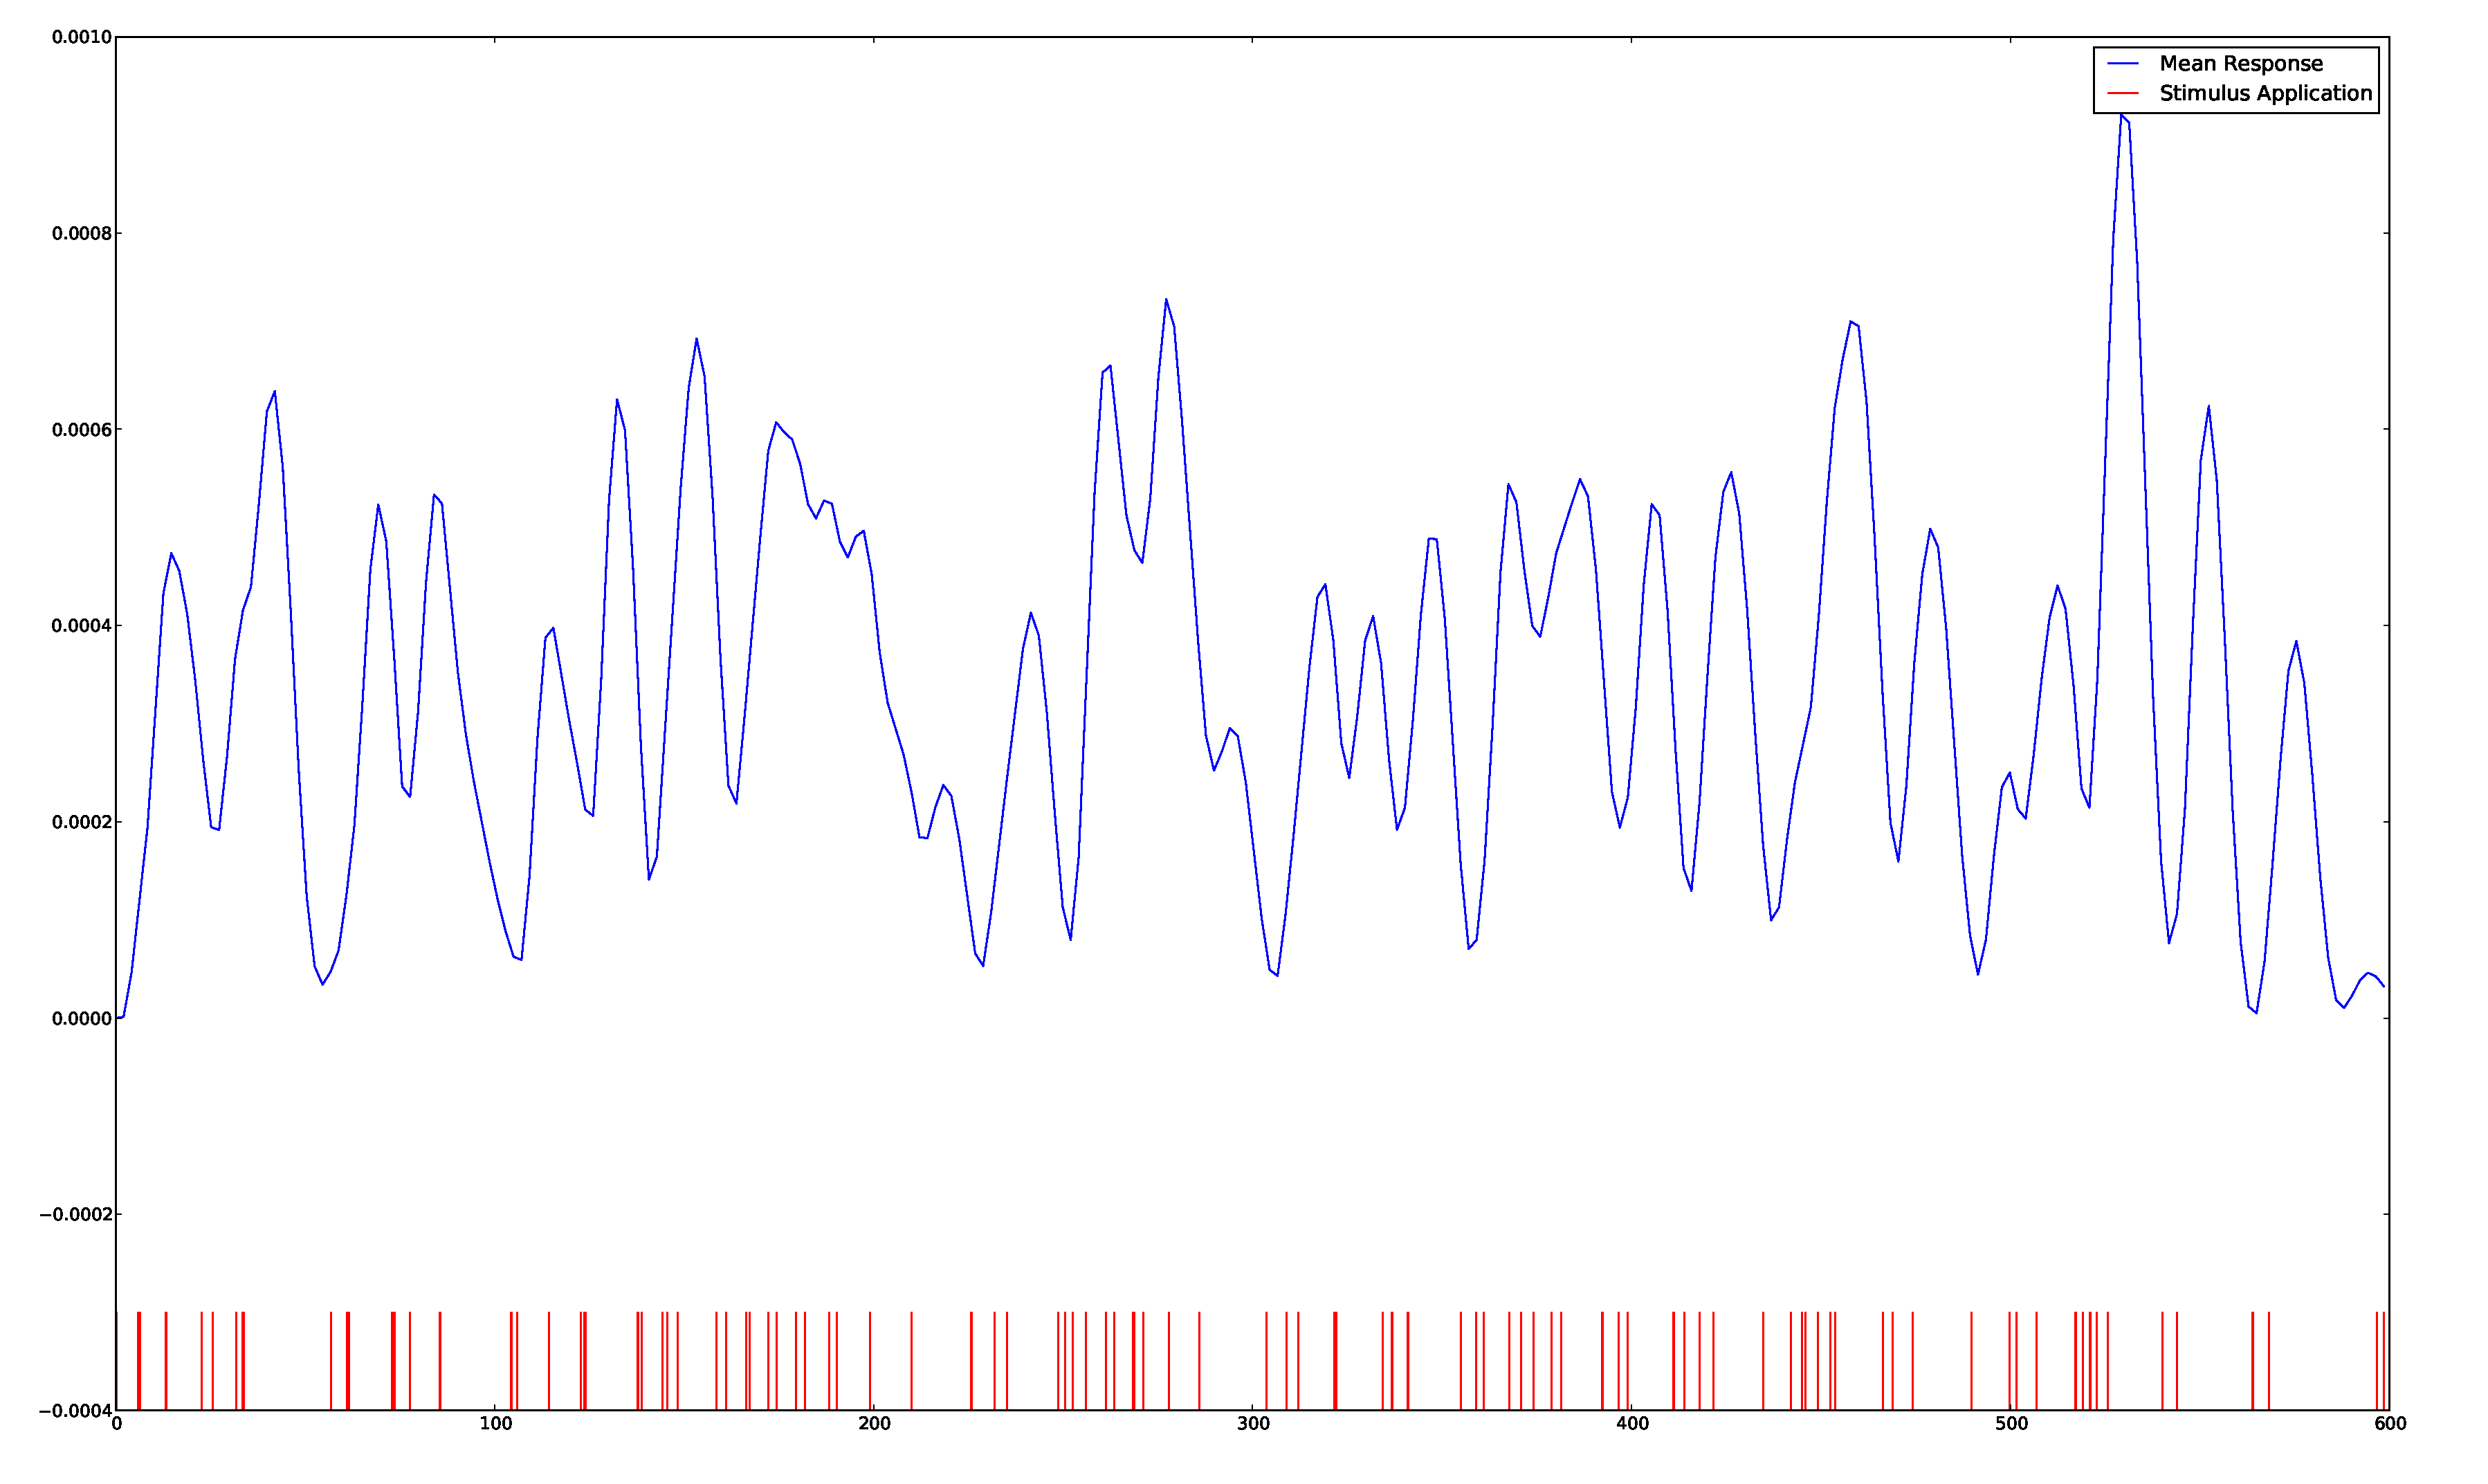
\includegraphics[trim=6cm 3cm 6cm 3cm,width=16cm]{images/mean_response_johnston}
\caption{Response to $.1s$ impulses with the mean parameters from \cite{Johnston2008}}
\end{figure}

Its likely that these differences are due to some difference in preprocessing,
although in \cite{Deneux2006} the signals were found to be peaking around
$1\%$, unlike \cite{Friston2000} which shows signals peaking at up to
$3\%$ or $4\%$. In my own tests, it seemed necessary for $\epsilon$ to
reach well over $1.5$ and $V_0$ to reach more than $.4$ to reach these
peaks; of course other methods may be equally able. 
Therefore, to account for these discrepancies, somewhat broader
distributions are used than the numbers used in \cite{Friston2000}
(which are widely used, \cite{Hu2009}). The 
priors used in the particle filter may be found in \autoref{tab:Prior}.

\begin{table}[t]
\centering
\begin{tabular}{|c || c | c | c |}
\hline 
Parameter & Distribution & $\mu$ & $\sigma$ \\
\hline
$\tau_0$ & Gamma & .98 & .25 \\
$\alpha$ & Gamma & .33 & .045\\
$E_0$    & Gamma & .34 & .03  \\
$V_0$    & Gamma & .04 & .03 \\
$\tau_s$ & Gamma & 1.54  & .25\\
$\tau_f$ & Gamma & 2.46  & .25\\
$\epsilon$ & Gamma & .7  & .6 \\
\hline
\end{tabular}
\caption{Prior distributions used in the particle filter.}
\label{tab:Prior} 
\end{table}

Note that although the mean remains the same for all the 
parameters other than $\epsilon$, the standard deviation is set
much higher to account for the disagreement between studies
(\autoref{tab:Params}). 
Because all the parameters are taken to be strictly positive, and the
standard deviations are approaching the mean, I used a gamma distribution.
This prevents the Gaussian from placing parameters in the nonsensical 
territory of negative activation, or negative time constants.

Another aspect of the prior is using enough particles to get a 
sufficiently dense approximation of the prior. For 7 dimensions,
getting a dense prior is difficult. Insufficiently
dense particles will result in inconsistent results. Of course the
processing time will scale up directly with the number of particles.
A dense initial estimate is important so that some particles land
near the solution; but as the variance decreases the number of 
particles needed decreases as well. Thus, as a heuristic, initially
the number of particles was set to 16,000, but after resampling,
the number of particles was dropped to 1,000. Typically during the 
first few measurements the variance dropped precipitously because
most particles were far from a solution.  The particles that are left are in a
much more compact location, allowing them to be estimated with 
significantly fewer particles. These numbers aren't set in stone,
and depending on the complexity of the system or desired accuracy
they could be changed; however, they seem to be the minimum that
will give consistent results.

\section{Resampling}
\label{sec:Resampling}
The algorithm for resampling is described in \autoref{sec:Particle Filter Resampling}.
When regularizing, the Gaussian kernel is convenient,
because it is simple to sample from and long tailed.
As discussed in \autoref{sec:Particle Filter Resampling},
as long as resampling is kept as a last resort, some over-smoothing
doesn't impair convergence. Therefore, for this work I chose a Gaussian kernel of
bandwidth equal to the original distribution's covariance. Obviously this will
apply a rather large amount of smoothing to the distribution; however, on average
resampling is only applied every 20 to 30 measurements, and because randomization
is being applied to model updates this gives the filter some mobility. 

Re-sampling is a not strictly necessary, but increases the effectiveness
of the particle filter by adjusting the support to emphasize areas
of higher probability. Re-sampling is slow because it requires re-drawing
all the particles. It also closes off avenues of investigation, and is
designed to over-smooth to prevent overly thinning the support. For all these
reasons, resampling was only performed when the $N_{eff}$ dropped below
50 (for 1000 particles).  As a measure against sharp drops in the $N_{eff}$ 
caused by a large spike in error, resampling was only performed when 
two consecutive low ($<50$) $N_{eff}$'s were found. 

\section{Choosing $P(y_k | x_k)$}
\label{sec:Methods Weighting Function}
The choice of $P(y_k | x_k)$ is the second most important design decision, behind 
the prior. While the conventional choice for an unknown distribution is the 
Gaussian, there are reasons why it may not be the best in this case.  
As noted in \autoref{sec:Introduction Noise}, the noise is not strictly Gaussian,
nor is it strictly Wiener. As with any unknown noise however, it is necessary 
to make some assumption. If the weighting function ($P(y_k | x_k)$) exactly
matches the measurement error, then the ideal particle filter will result.
Particles with $x_k$'s that repeatedly estimate $y_k$ with large residual 
will quickly have weights near 0. Thus, a weighting function that
exactly matches $P(Y(t) | X(t))$ will easily, and correctly throw out incorrect
particles.  The cost of choosing an overly broad distribution for this
function is slow convergence.  On the other hand, an overly thin 
distribution will lead to particle deprivation (all particles
being zero-weighted).  I tested several weighting
functions: in addition to the Gaussian I also tested the Laplace and Cauchy
distributions, both of which have much wider tales than the Gaussian. 
Wider tailed distributions don't down-weight
particles as fast; and converge more slowly (and perhaps more accurately). 
The Laplace distribution also has the
benefit of a non-zero slope at the origin; which means that even
it will distinguish between particles even near the origin.

After trial and error, for this work I chose a zero-mean Gaussian with standard deviation 
of $.005$. While I made some attempts to automatically set the standard 
deviation, results were often unpredictable. If the weight function and scale aren't
fixed across voxels, very noisy time series with no actual signal 
converged to nonsensical results. 
In the future, it may be possible to set the standard deviation by
taking a small sample from resting data and using the sample standard deviation.
Since this is the first attempt at using particle filters for modeling the 
BOLD model, in this work I set the standard deviation manually at $.005$,
because it gave the best consistency. 

\subsection{Runtime}
The run-time for a single voxel depends on the several factors. First, the
overall length of the signal being analyzed. For 1000 measurements it takes
about 6 minutes. On the other hand, in real circumstances the
length is only around 150 measurements and takes around 40 seconds (for 1000 
particles, 1500 integration points and a Quad Core CPU). The size of 
local linearization steps are also crucial although going above .001 seconds
per step is not recommended. In most cases millisecond resolution
is fine; however, when generating simulated data I found that at times it was
still not enough every once. This is problematic in the actual particle
filter since, given the large number of simultaneous integrations taking 
place, its probable that a few particles will fail and be unfairly thrown away.
To prevent such events, 1500 integration points per second were used throughout
the tests. 

Another crucial factor for run time is how long before the first re-sampling 
occurs. Because the prior is represented initially with significantly more
particles, if for some reason the effective
number of particles stays high, resampling could take a long time to occur.
For this reason, rather than allowing the particle filter to continue on 
with this large number of particles, after 20 seconds have passed the
algorithm forces resampling. The choice of 20 seconds is 
arbitrary, but at the very least it gives a more optimized version of the
prior. 


\chapter{Results}

\section{Simulation}
I performed two types of simulations. First, I simulated a single BOLD time-series based
on a randomly selected set of model parameters. Second I used a modified version of the
FSL tool possum to generate a noisy FMRI image. 

\subsection{Single Timeseries}
This process was relatively straight forward,
given the state-space equations for the BOLD signal. After a "true" signal was generated,
I then added a identically and independently distributed (I.I.D.) Gaussian noise and a Wiener
process with Gaussian I.I.D. steps. Finally a carrier level was added, since BOLD is typically
measured as a \% difference from the
base level. Adding a carrier level meant that the exact same algorithm which was used for 
real data could be used for the simulated data. 

Once this noisy simulated time series was generated, the particle filter algorithm
 was run on this single timeseries image. In order to find the best setting for the
particle filter I ran quite a few tests. Here I will include two sets of tests 
to determine the power of the particle filter in modeling. The first test is
low noise $\{\sigma_y = .001, \sigma_x = .0005\}$, while the second set of
tests had noise of $ \{\sigma_y = .01, \sigma_x = .005\} $, where $\sigma_y$ is the
measurement noise, and $\sigma_x$ is the wiener step size. Both signals used the
parameters ($\tau_0 = 1.45, \alpha = .3, E_0 = .47, V_0 = .044, \tau_s = 1.94, \tau_f = 1.99, \epsilon = 1.8$).
The particle filter used the parameters defined in \autoref{tab:Prior} (\autoref{sec:PriorDistrib}),
thus the particle filter was not centered over the correct values. 

\subsubsection{Low Noise Simulation}
For the low noise case, the ten realization are shown in \autoref{fig:LowNoiseRealization}.
\begin{figure}
\label{fig:LowNoiseRealization}
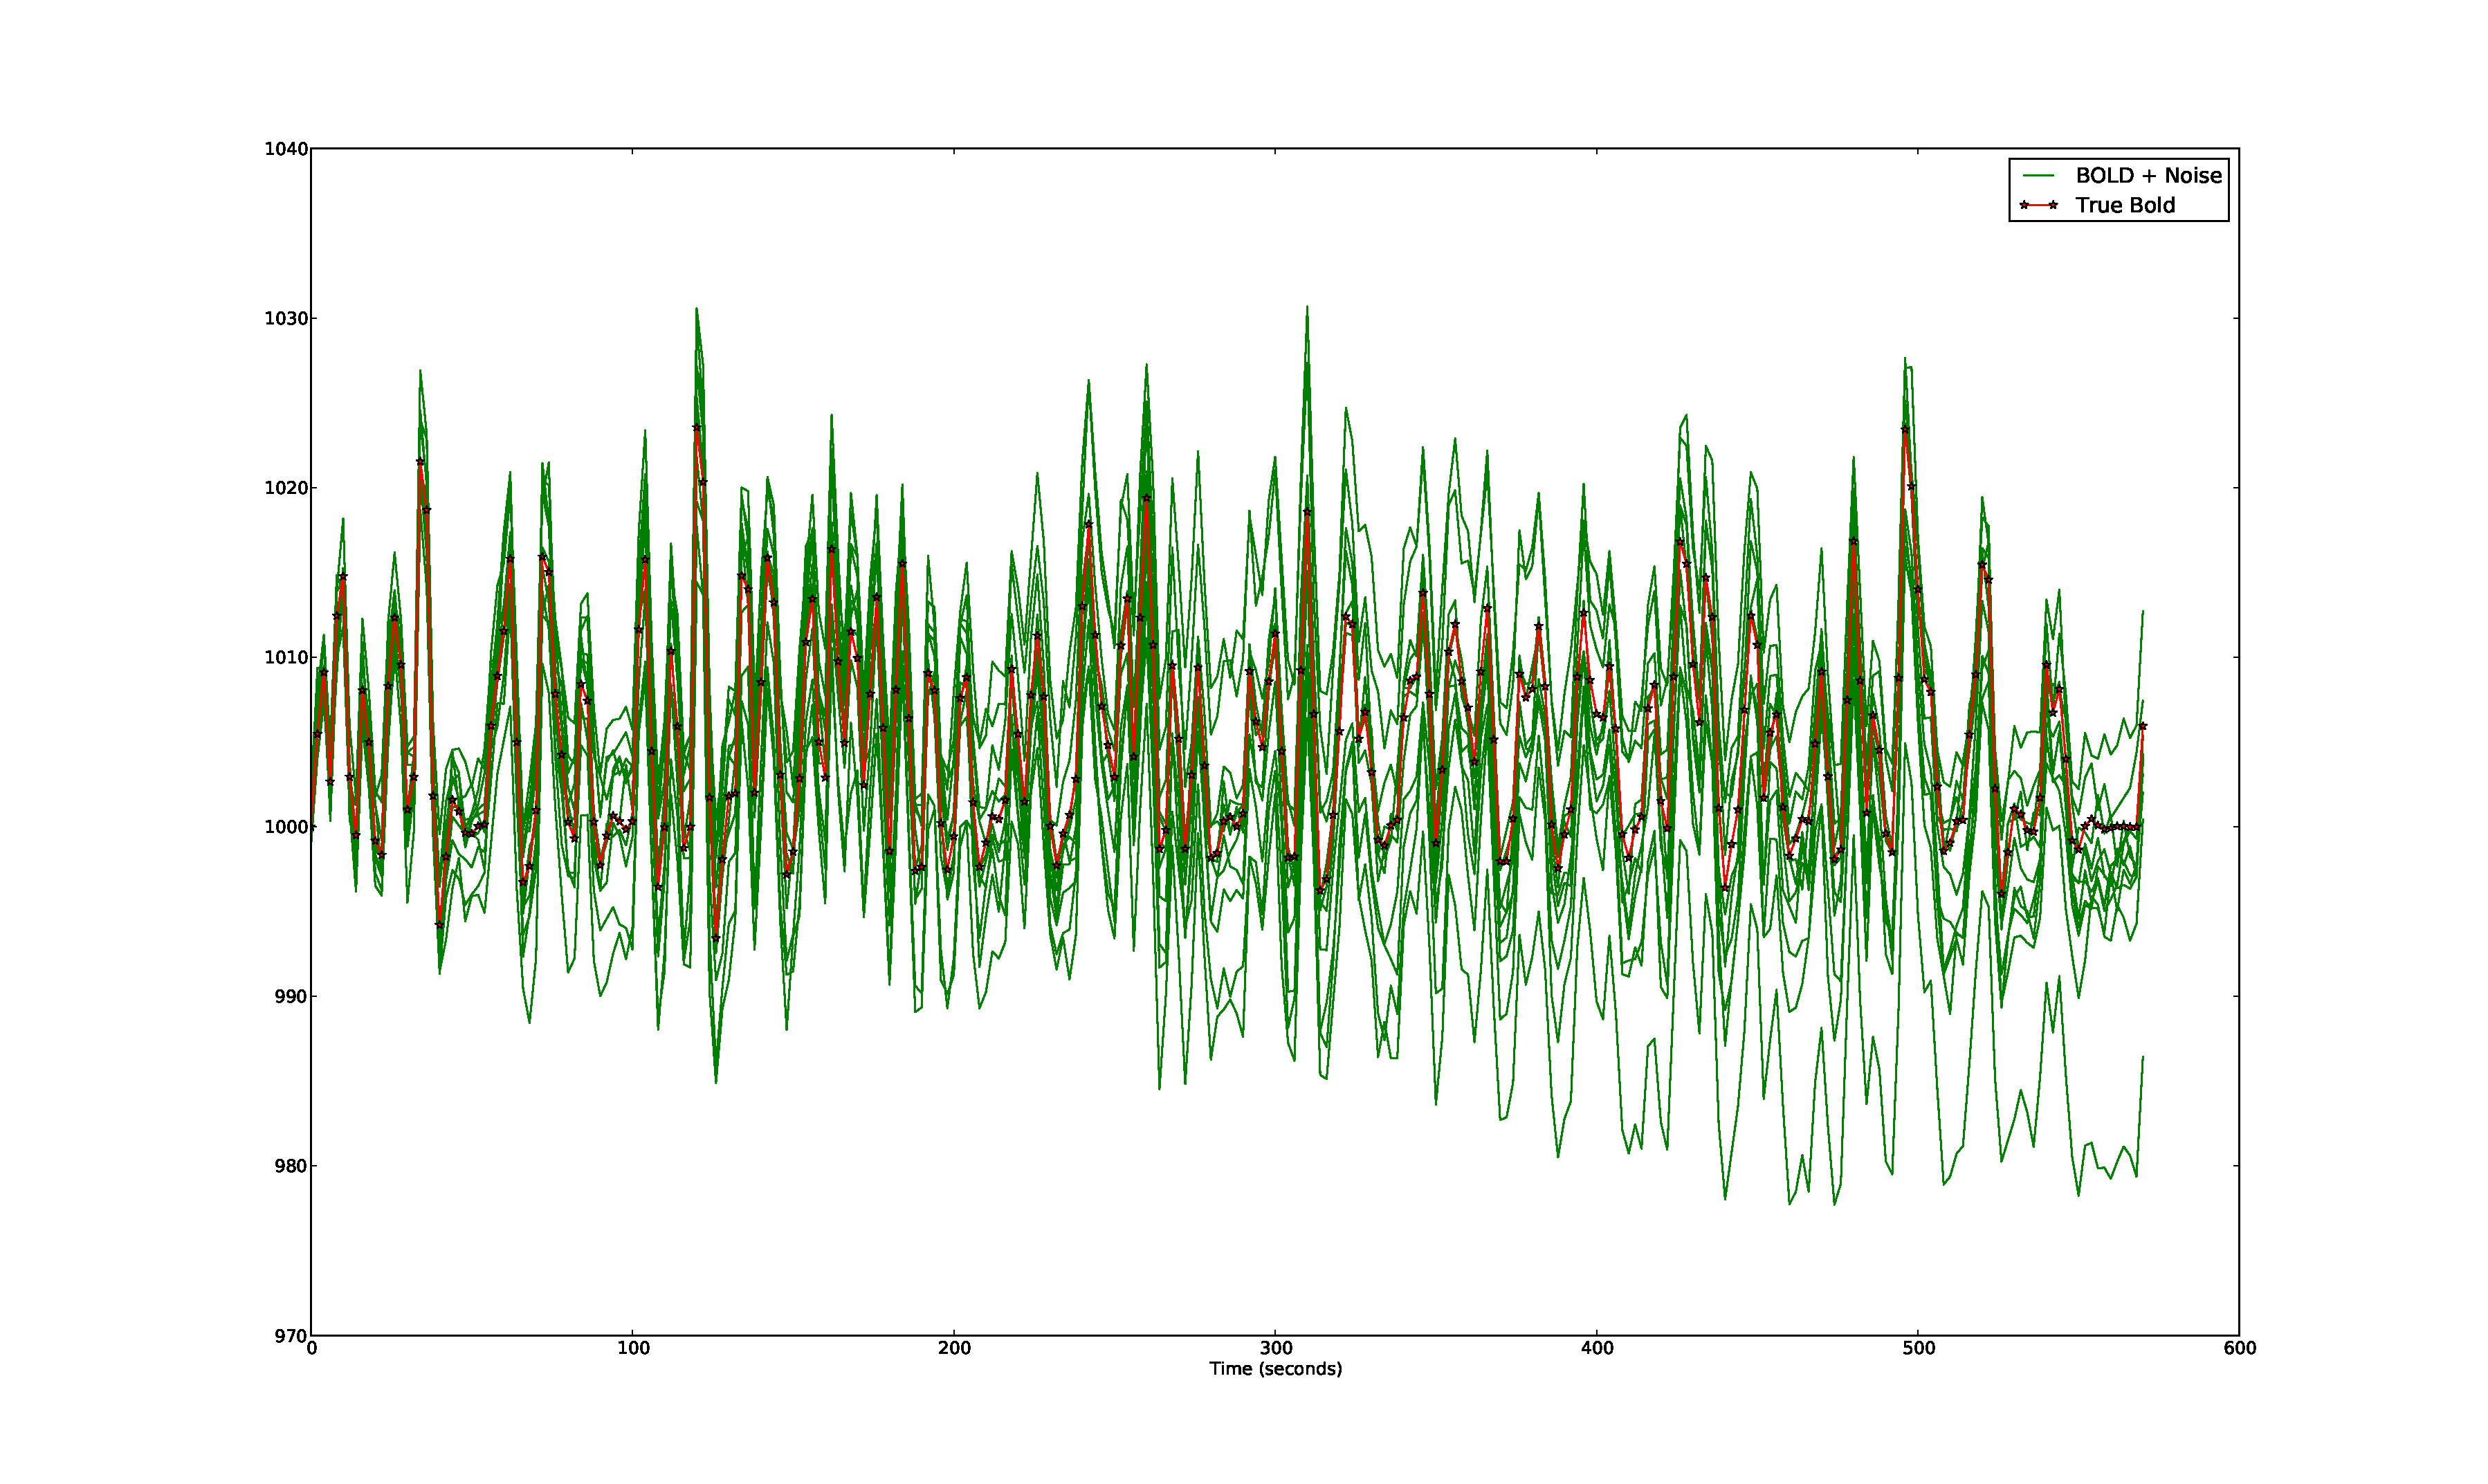
\includegraphics[trim=6cm 3cm 6cm 3cm,width=16cm]{images/realization_lownoise}
\caption{Test Signals with low noise compared to the clean signal}
\end{figure}

The resulting fits compared to the \emph{true} BOLD signal are shown in \autoref{fig:FitComparisonLowNoise}.
The fits are good, but the noise is relatively low. The preprocessed signal compared
to the true BOLD signal is shown in \autoref{fig:PreprocessedLowNoise}.

\begin{figure}
\label{fig:PreprocessedLowNoise}
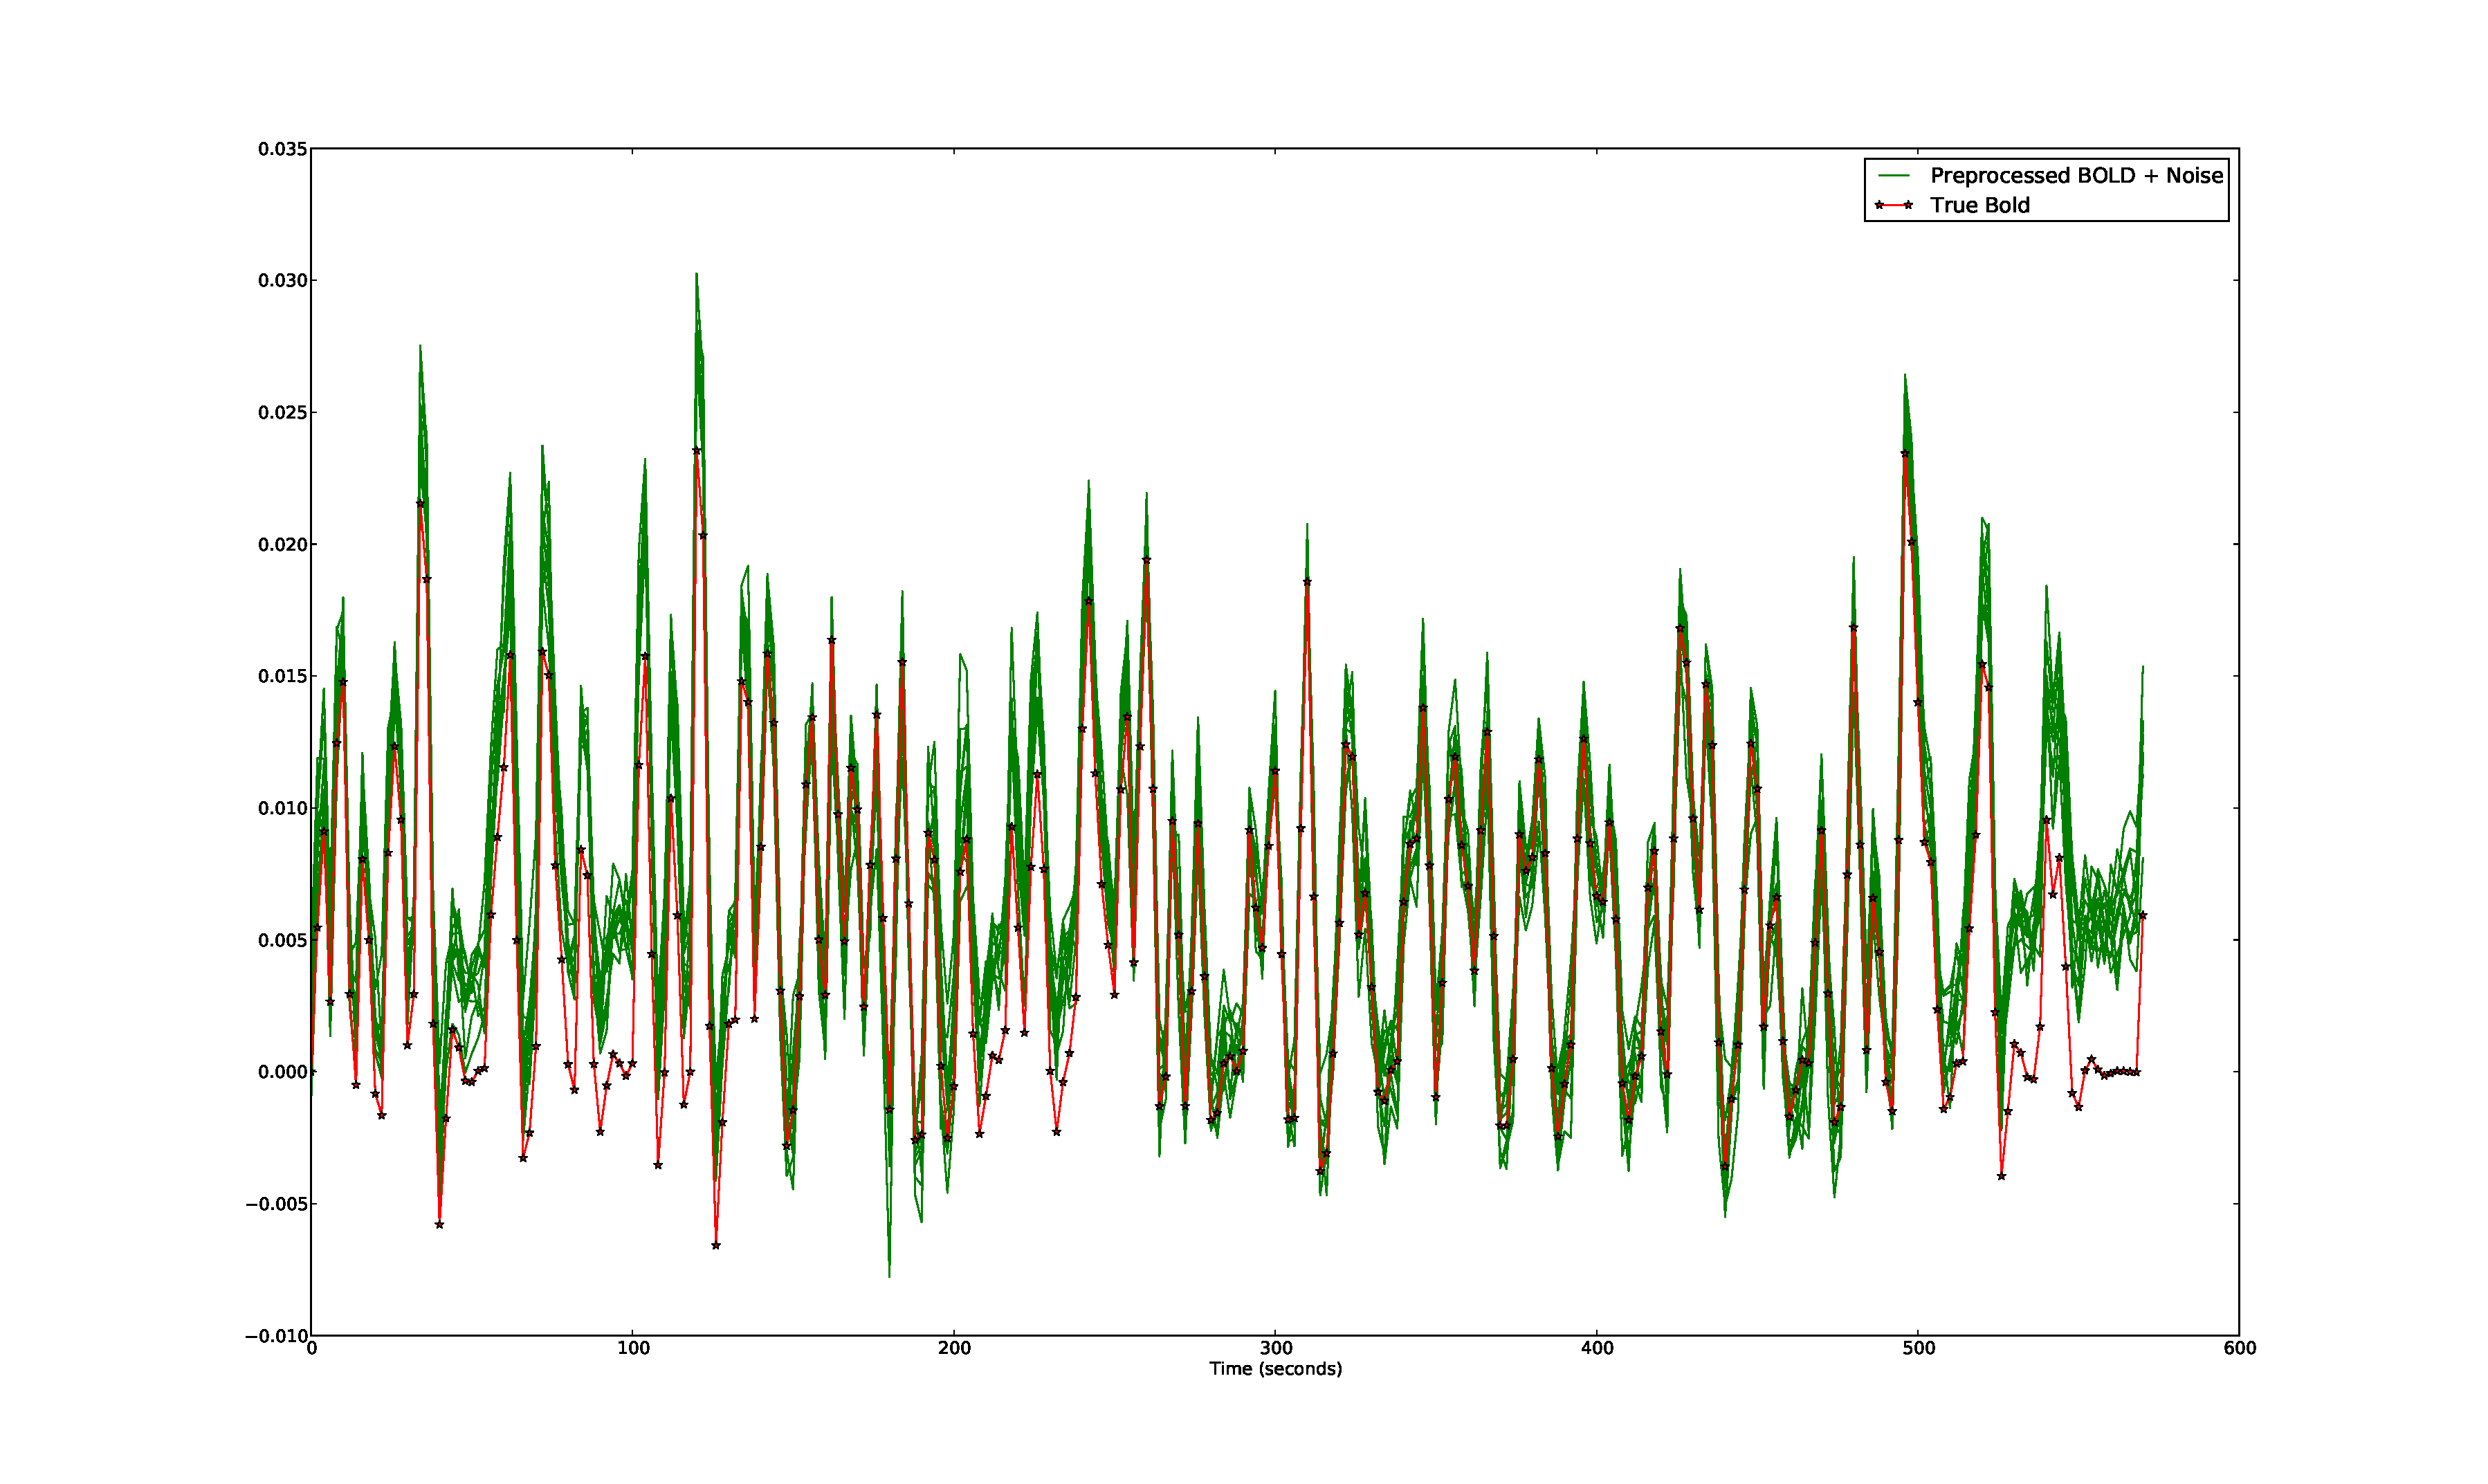
\includegraphics[trim=6cm 3cm 6cm 3cm,width=16cm]{images/preprocessed_lownoise}
\caption{A comparison of the preprocessed signals for the low noise case.}
\end{figure}

The preprocessing consists of several steps, which are discussed in detail in \autoref{sec:Preprocessing}.
Obviously the spline struggles a little bit at the end, as the graph shows, although 
overall the fit is pretty well. Finally, the set of fits to the preprocessed data, and in 
essence to the "true" BOLD signal is shown in \autoref{fig:FitComparisonLowNoise}.

\begin{figure}
\label{fig:FitComparisonLowNoise}
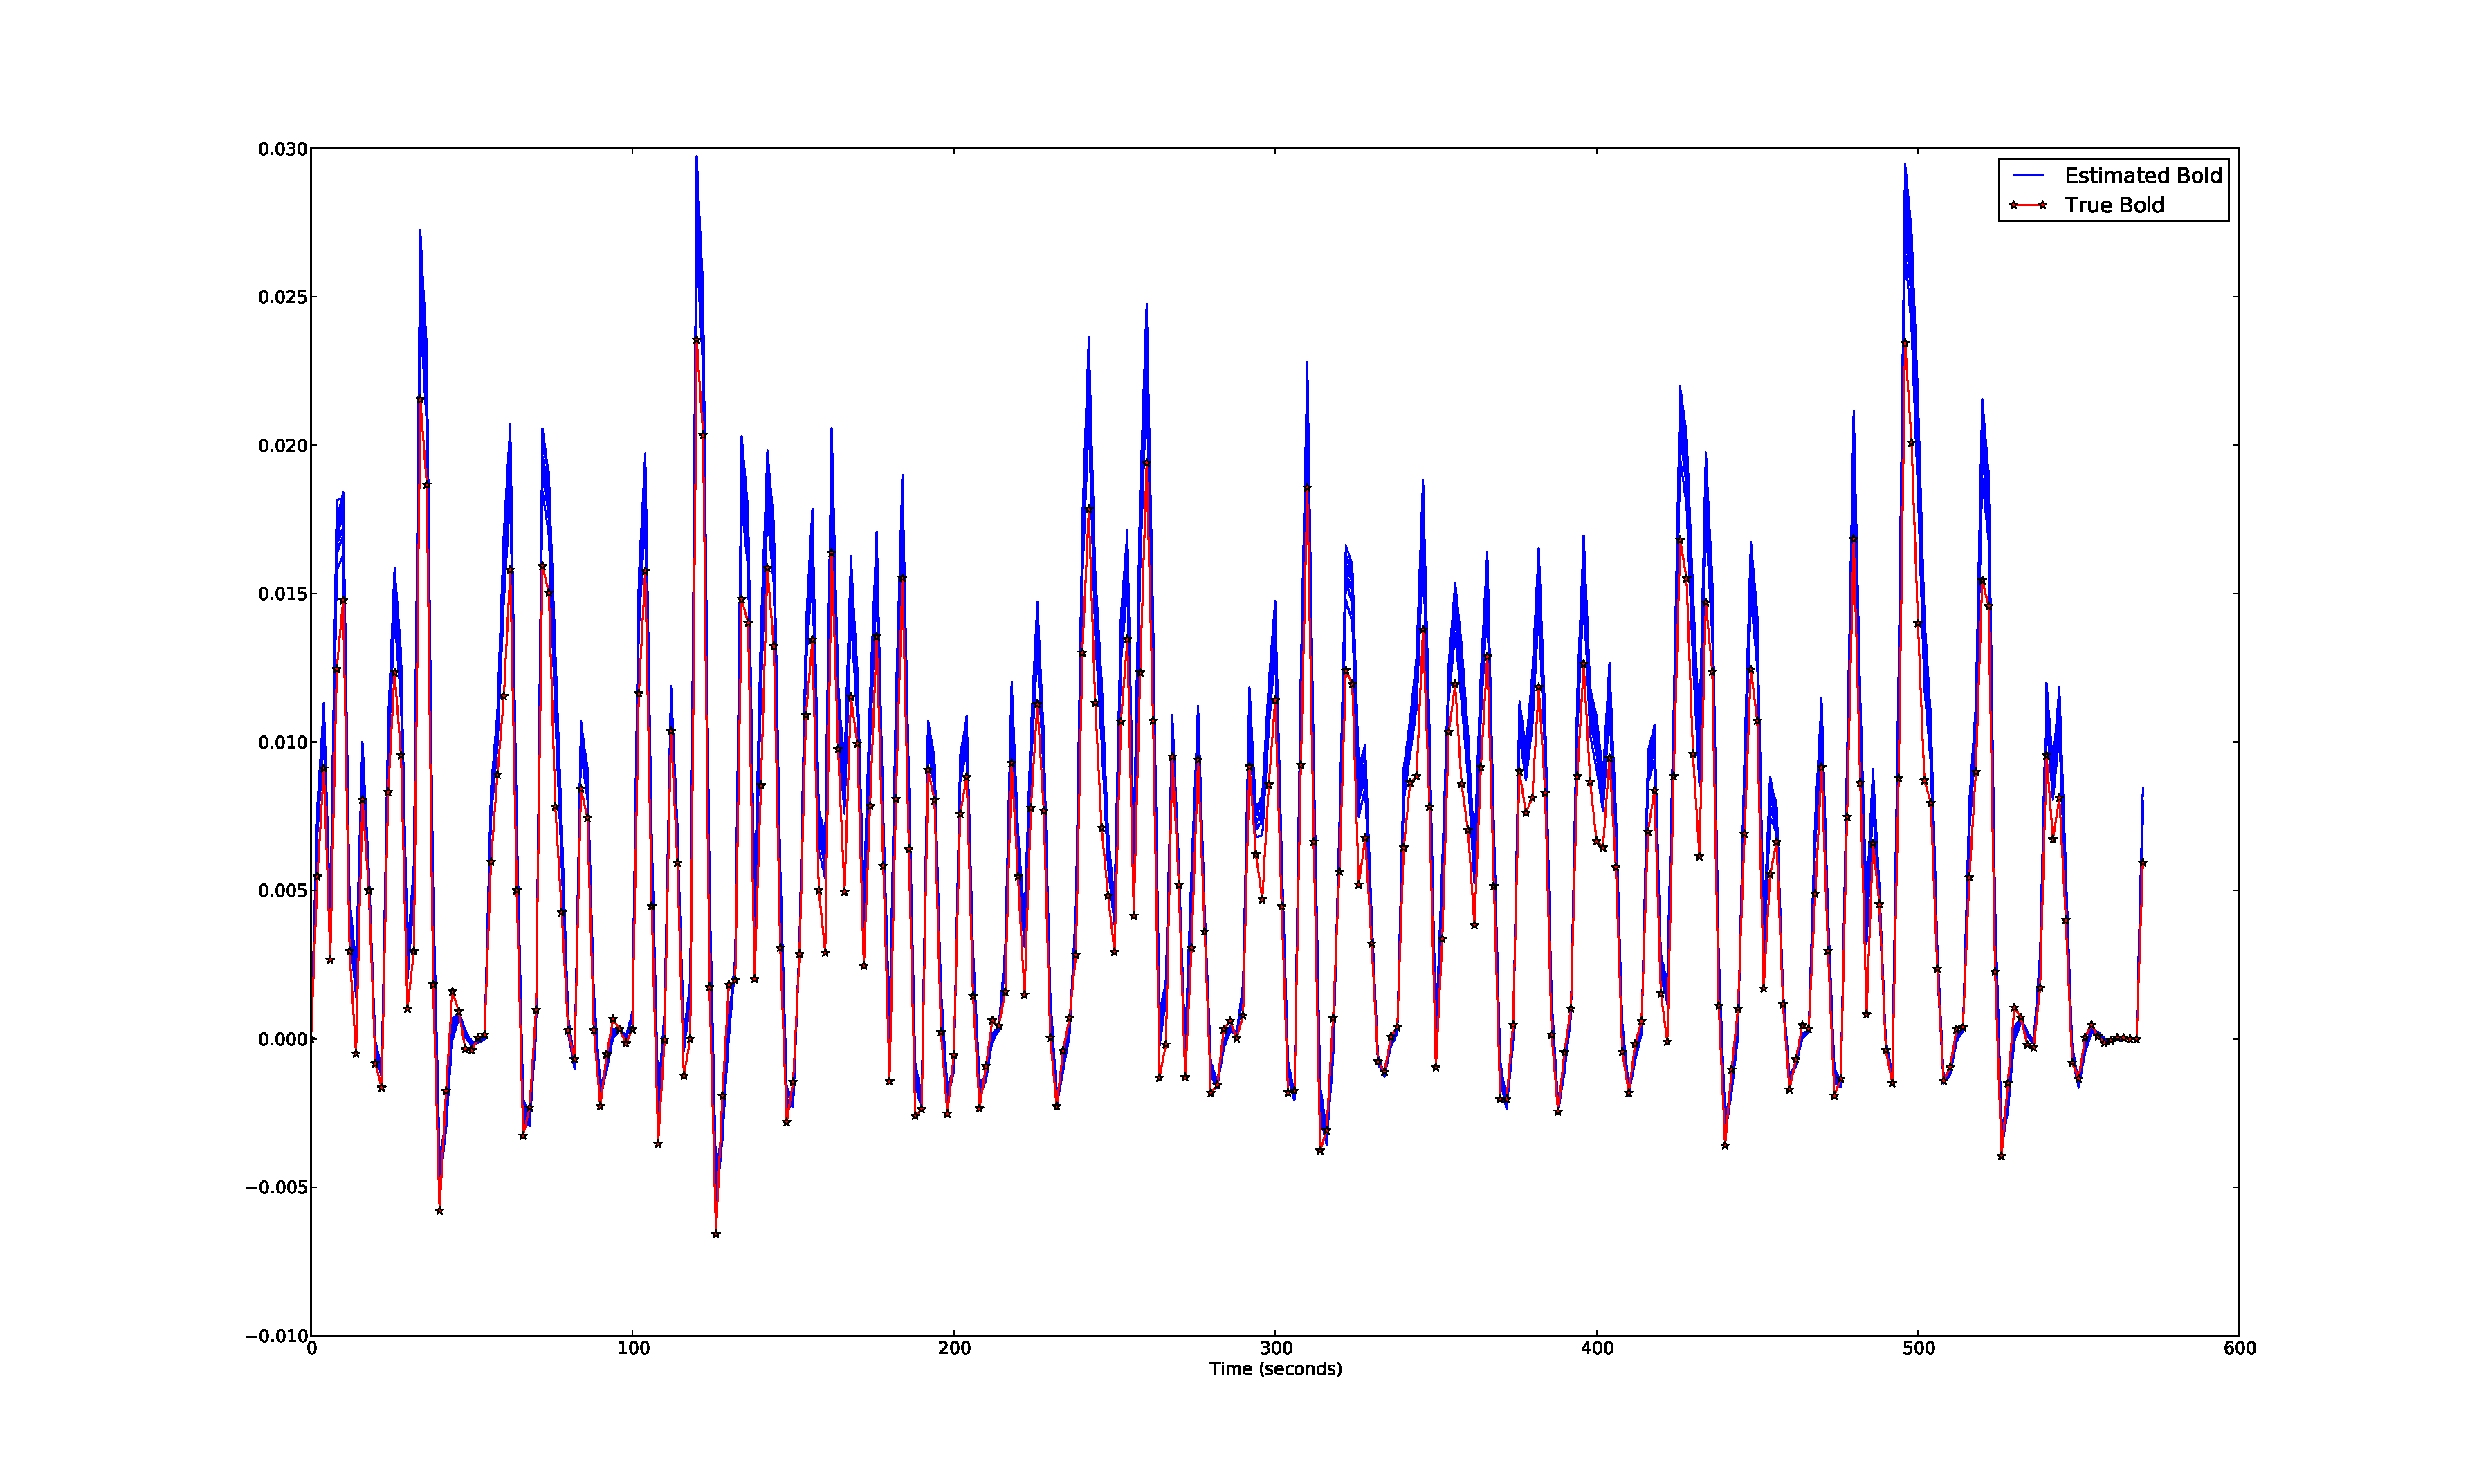
\includegraphics[trim=6cm 3cm 6cm 3cm,width=16cm]{images/comparison_lownoise}
\caption{A comparison of the fitted signals for the low noise case.}
\end{figure}

It becomes clear now the reason for the term particle filter. In several locations the output
of the particle filter looks like a filtered version of the input. For instance toward the
end, the estimates stay flat in spite of the preprocessed data drifting off a bit. By
this point, the algorithm had converged sufficiently to know that that wasn't possible.
A similar circumstance occurs at 100 seconds in. In general the fits are good, although because
of the slightly higher signal levels in the preprocessed signals, the fits tend to overestimate
the peak a bit. The final parameter sets are shown in \autoref{tab:LowNoiseParams}
\begin{table}[t]
\centering
\begin{tabular}{|c | c | c | c | c | c | c | c | c | c |}
\hline 
$\tau_0$ & $\alpha$ & $E_0$    & $V_0$    & $\tau_s$ & $\tau_f$ & $\epsilon$  & $ \sum \tau $ & $\sqrt{MSE}$ (Res.) &$\sqrt{MSE}$\\
\hline 
\rowcolor[gray]{.8}
1.45 & .3 & .47 & .044 & 1.94 & 1.99 & 1.8  & 5.38 &  & \\
\hline 
\hline 
1.22214 & 0.3449 & 0.33462 & 0.07138 & 1.60446 & 2.27529 & 1.59454 & 5.10189  &  0.00321067  & 0.00987647  \\
1.37493 & 0.33183 & 0.36296 & 0.07327 & 1.64076 & 2.10299 & 1.57627 & 5.11867 &  0.00305475  & 0.00993227  \\
1.16604 & 0.32205 & 0.34057 & 0.08217 & 1.64768 & 2.35351 & 1.24515 & 5.16722 &  0.00328932  & 0.00967961  \\
1.23176 & 0.32707 & 0.34028 & 0.07961 & 1.62698 & 2.18519 & 1.30326 & 5.04394 &  0.00284719  & 0.00912005  \\
1.1832 & 0.31787 & 0.34718 & 0.0821 & 1.54961 & 2.29115 & 1.27817 & 5.02396   &  0.00300634  & 0.00971258  \\
1.1424 & 0.33395 & 0.34725 & 0.07366 & 1.62208 & 2.29084 & 1.4025 & 5.05531   &  0.00283287  & 0.00948483  \\
1.30041 & 0.3596 & 0.35643 & 0.07679 & 1.56406 & 2.13234 & 1.60338 & 4.99681  &  0.00302802  & 0.01021885  \\
1.24008 & 0.34601 & 0.33978 & 0.08903 & 1.64989 & 2.23655 & 1.29004 & 5.12651 &  0.00304378  & 0.01007964  \\
1.1709 & 0.32739 & 0.34644 & 0.08255 & 1.53734 & 2.28262 & 1.37828 & 4.99087  &  0.00334488  & 0.01032886  \\
1.18967 & 0.34344 & 0.33554 & 0.07976 & 1.53582 & 2.30746 & 1.42774 & 5.03295 &  0.00317542  & 0.01001503  \\
1.184 & 0.34053 & 0.35017 & 0.08917 & 1.61025 & 2.27926 & 1.16448 & 5.07352   &  0.00288855  & 0.00950536  \\
\hline                                                                           
1.21868 & 0.33588 & 0.34557 & 0.07995 & 1.59899 & 2.24884 & 1.38762 & 5.06651 & 0.00306562     & 0.00981396 \\
\hline 
\end{tabular}
\caption{Estimated Parameters on 10 different runs with low noise. First row is the true parameters,
last is mean over the 10 runs. The $\sqrt{MSE}$ (Res.) is the square root of the mean square of the
residuals. Essentially this is the is the MSE between the estimated signal and the noisy signal which 
was available to the particle filter. Square root of MSE is the actual \emph{error}, with the true signal,
which of course was not available to the particle filter.}
\label{tab:LowNoiseResults} 
\end{table}

There are a few things worth noting here. First the time constants vary greatly across
runs with different noise realizations, yet the sum of the individual time constants
, $\tau_f$, $\tau_s$ and $\tau_0$ seem to be more consistent. In general the 
time constants are falling short of the true time constant. This could be a limitation
based on the prior distribution (which notably has mean values below the values used
in the simulation) or it could be caused by the delayed benefit of having a 
correct time constant. Even if one particle has a better time constant than another, if
the difference isn't severe, by the time this makes a difference in the weight, the 
particle with the better $\tau$ will have been weighted based on other parameters several
times. Another interesting result in the huge variation in the levels of $V_0$. In general,
with this admittedly small amount of noise, it would appear that the relation between a set
of parameters/stimuli with the output is not injective. In other words, it would appear
that a timeseries is not unique to a set of parameters. This is good justification that 
simultaneous blood volume or tagged flow calculations with the conventional FMRI 
could definitely benefit the model. 

\begin{table}[t]
\centering
\begin{tabular}{|c | c  c  c  c  c  c  c |}
\hline 
  & $\tau_0$ & $\alpha$ & $E_0$    & $V_0$    & $\tau_s$ & $\tau_f$ & $\epsilon$ \\
\hline 
\rowcolor[gray]{.8} $\tau_0$ &   0.0189481 & -0.0014269 & -0.0011267 & -1.13e-05 & -0.0025616 & -0.0189559 & 0.0070405 \\
$\alpha$ &                       -0.0014269 & 0.0026716 & 9.93e-05 & -0.0002041 & -0.0008632 & -0.0016823 & 0.0071891 \\
\rowcolor[gray]{.8} $E_0$    &   -0.0011267 & 9.93e-05 & 0.0010701 & -0.0002277 & -0.0001177 & 0.0001013 & 0.0016972 \\
$V_0$    &                       -1.13e-05 & -0.0002041 & -0.0002277 & 0.0005401 & 4.3e-06 & 4.56e-05 & -0.0080494 \\
\rowcolor[gray]{.8} $\tau_s$ &   -0.0025616 & -0.0008632 & -0.0001177 & 4.3e-06 & 0.0128056 & 0.012878 & -0.005516 \\
$\tau_f$ &                       -0.0189559 & -0.0016823 & 0.0001013 & 4.56e-05 & 0.012878 & 0.0416927 & -0.0158182 \\
\rowcolor[gray]{.8} $\epsilon$&  0.0070405 & 0.0071891 & 0.0016972 & -0.0080494 & -0.005516 & -0.0158182 & 0.1567165 \\
\hline 
\end{tabular}
\caption{Typical Covariance matrix of the parameters at the end of a run.}
\label{tab:CovSim} 
\end{table}

\begin{figure}[H]
\subfigure[Converging histogram for $\tau_0$, $\alpha$, $E_0$, and $V_0$ of the first run, low noise simulation.]
{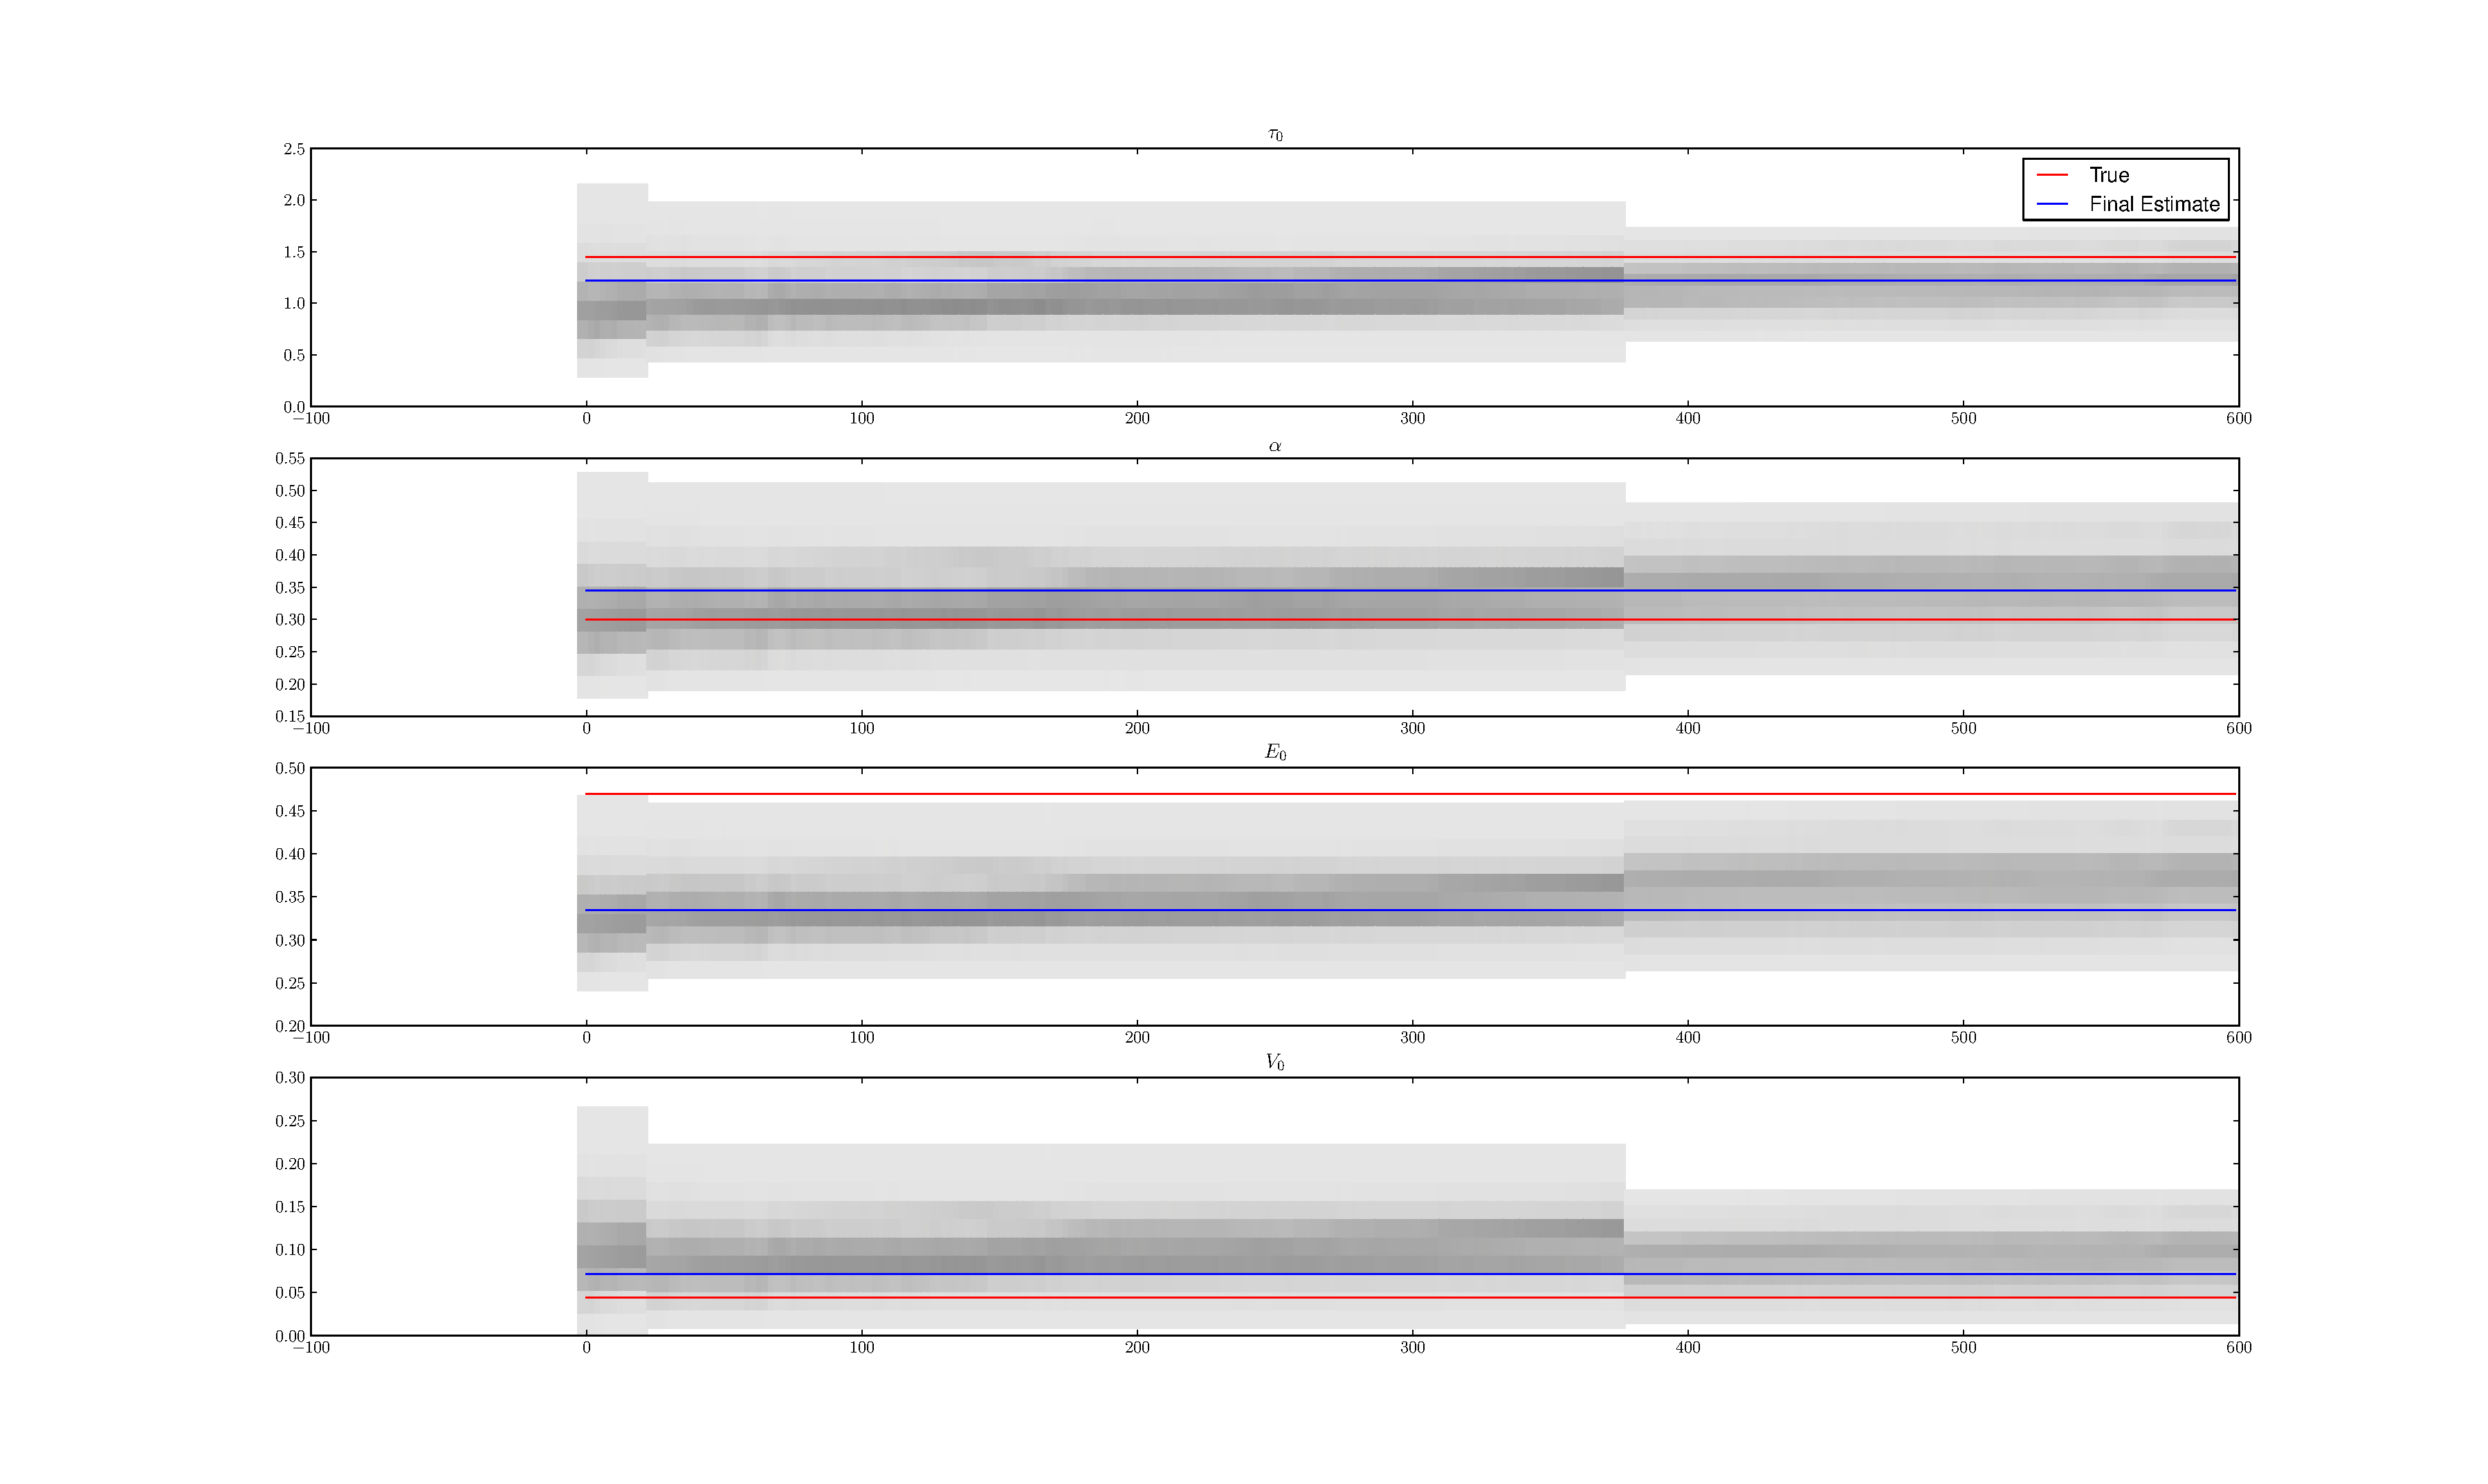
\includegraphics[trim=7cm 4cm 7cm 4cm, width=15cm]{images/converge_lownoise1}}\\

\subfigure[Converging histogram for $\tau_s$, $\tau_f$, $\epsilon$, and $V$ of the first run, low noise simulation.]
{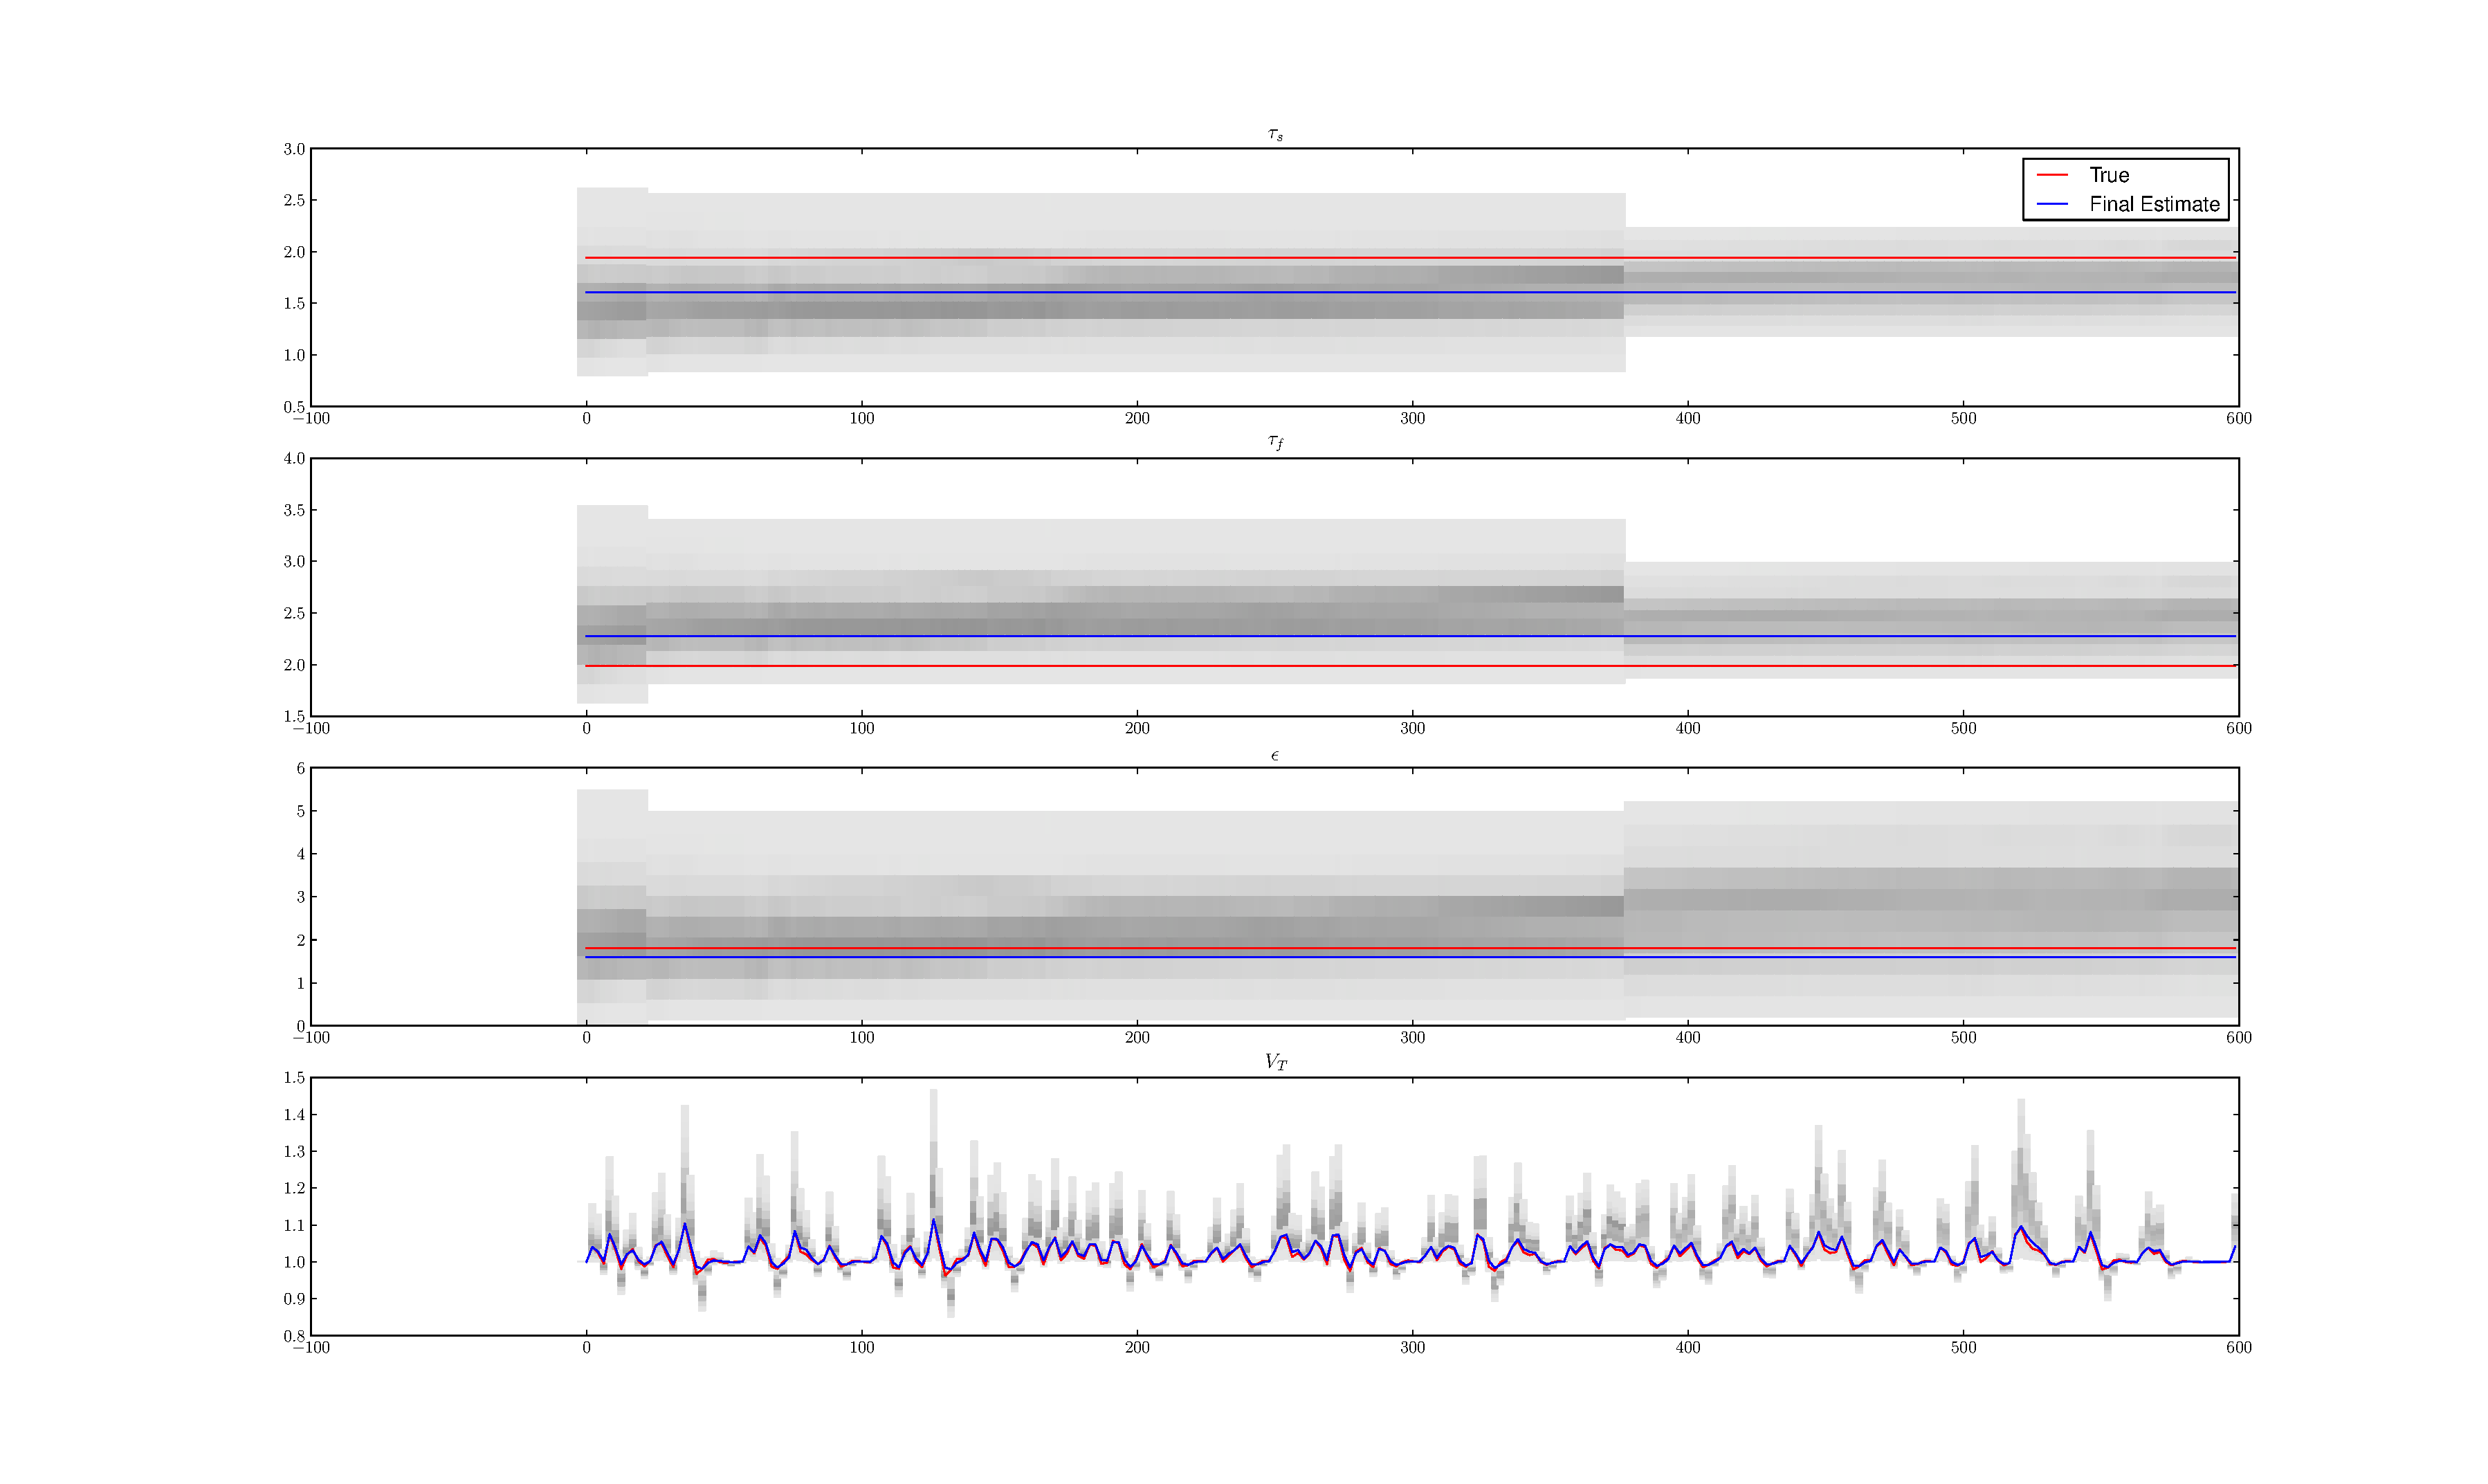
\includegraphics[trim=7cm 4cm 7cm 1cm, width=15cm]{images/converge_lownoise2}}\\
\end{figure}

\begin{figure}
\subfigure[Converging histogram for $Q$, $S$, $F$, and $BOLD$ of the first run, low noise simulation.]
{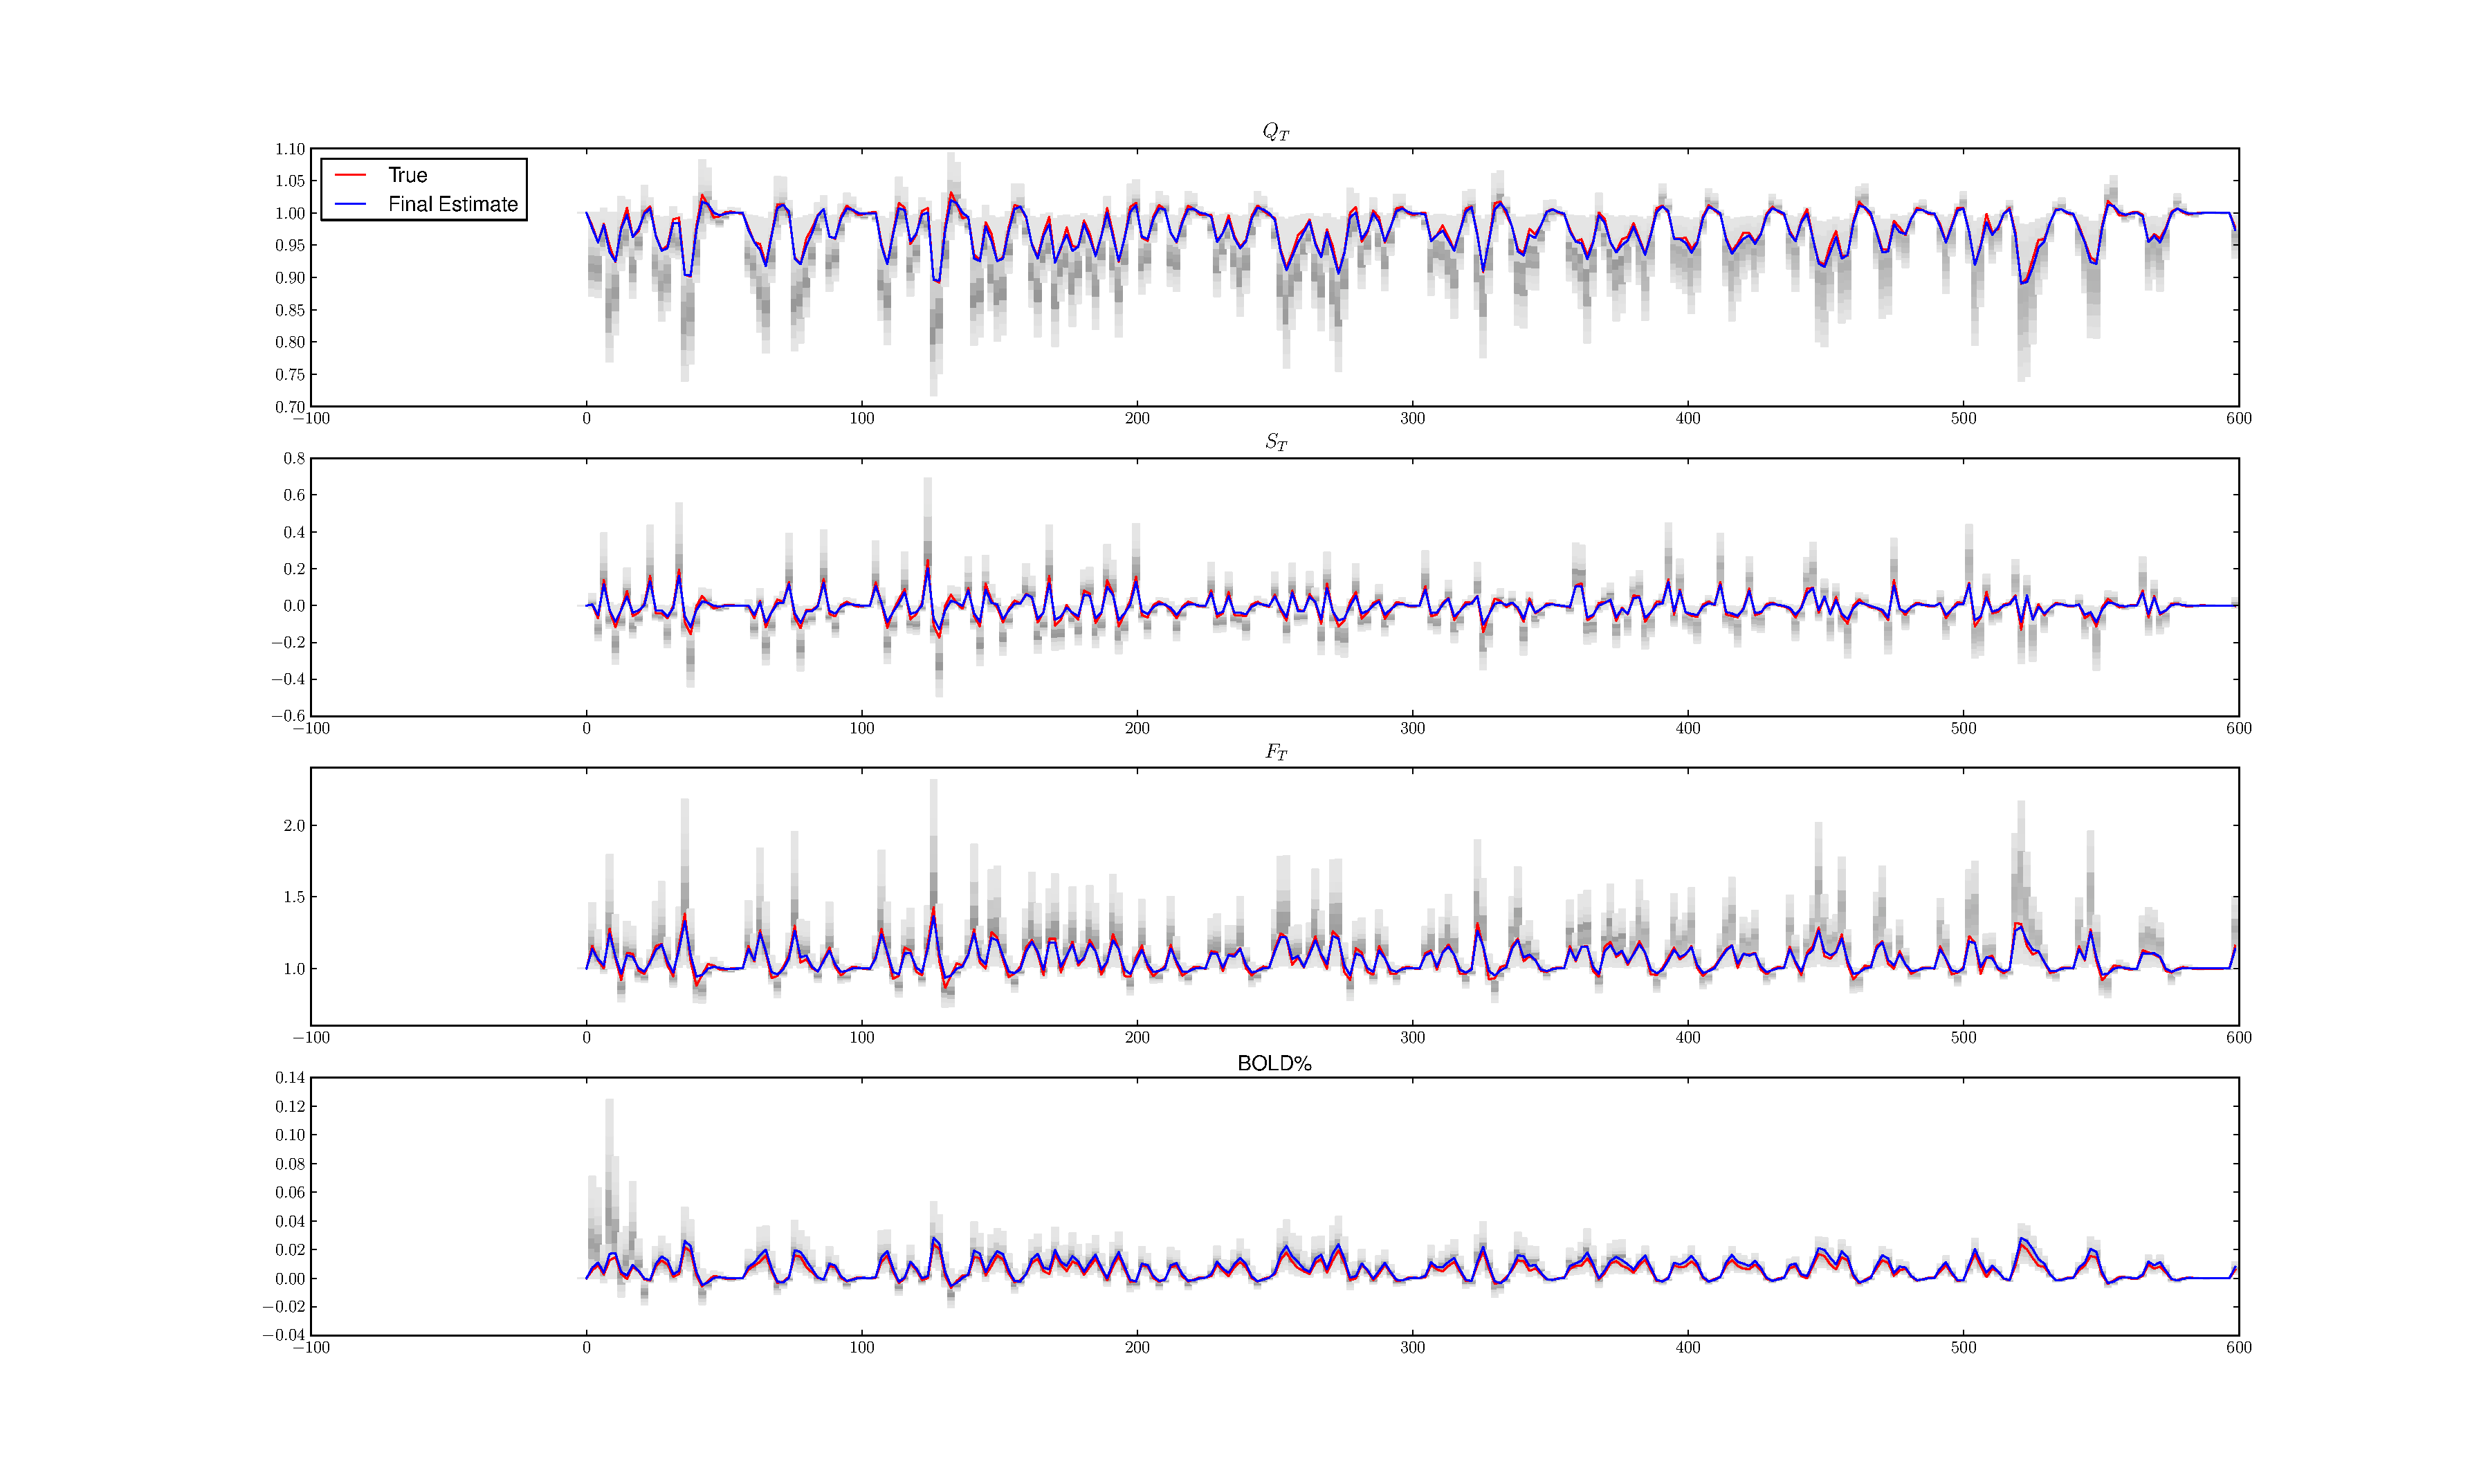
\includegraphics[trim=7cm 2cm 7cm 2cm, width=15cm]{images/converge_lownoise3}}
\label{fig:LowNoiseHist}
\end{figure}
The covariance matrix (\autoref{tab:CovSim}) also confirms the idea that the $\tau$ parameters are interchangeable
as far as the BOLD signal goes. Notice the covariance of $\tau_f$ and $\tau_0$ is $-0.019$ whereas
the variance of $\tau_0$ and $\tau_f$ are $0.019$ and $0.04$ respectively. Clearly they are
related. The convergence properties of the first run in \autoref{tab:LowNoiseResults} may be
viewed in \autoref{fig:LowNoiseHist}.

\subsubsection{High Noise Simulation}
For the high noise simulation, the exact same procedure was performed again, but with 
measurement error and drift standard
deviations an order of magnitude higher. The noisy signals versus the base signal are shown
in \autoref{fig:HighNoiseRealization} and the preprocessed signals which the particle
filter attempt to fit are in \autoref{fig:PreprocessedHighNoise}.
\begin{figure}[H]
\label{fig:LowNoiseRealization}
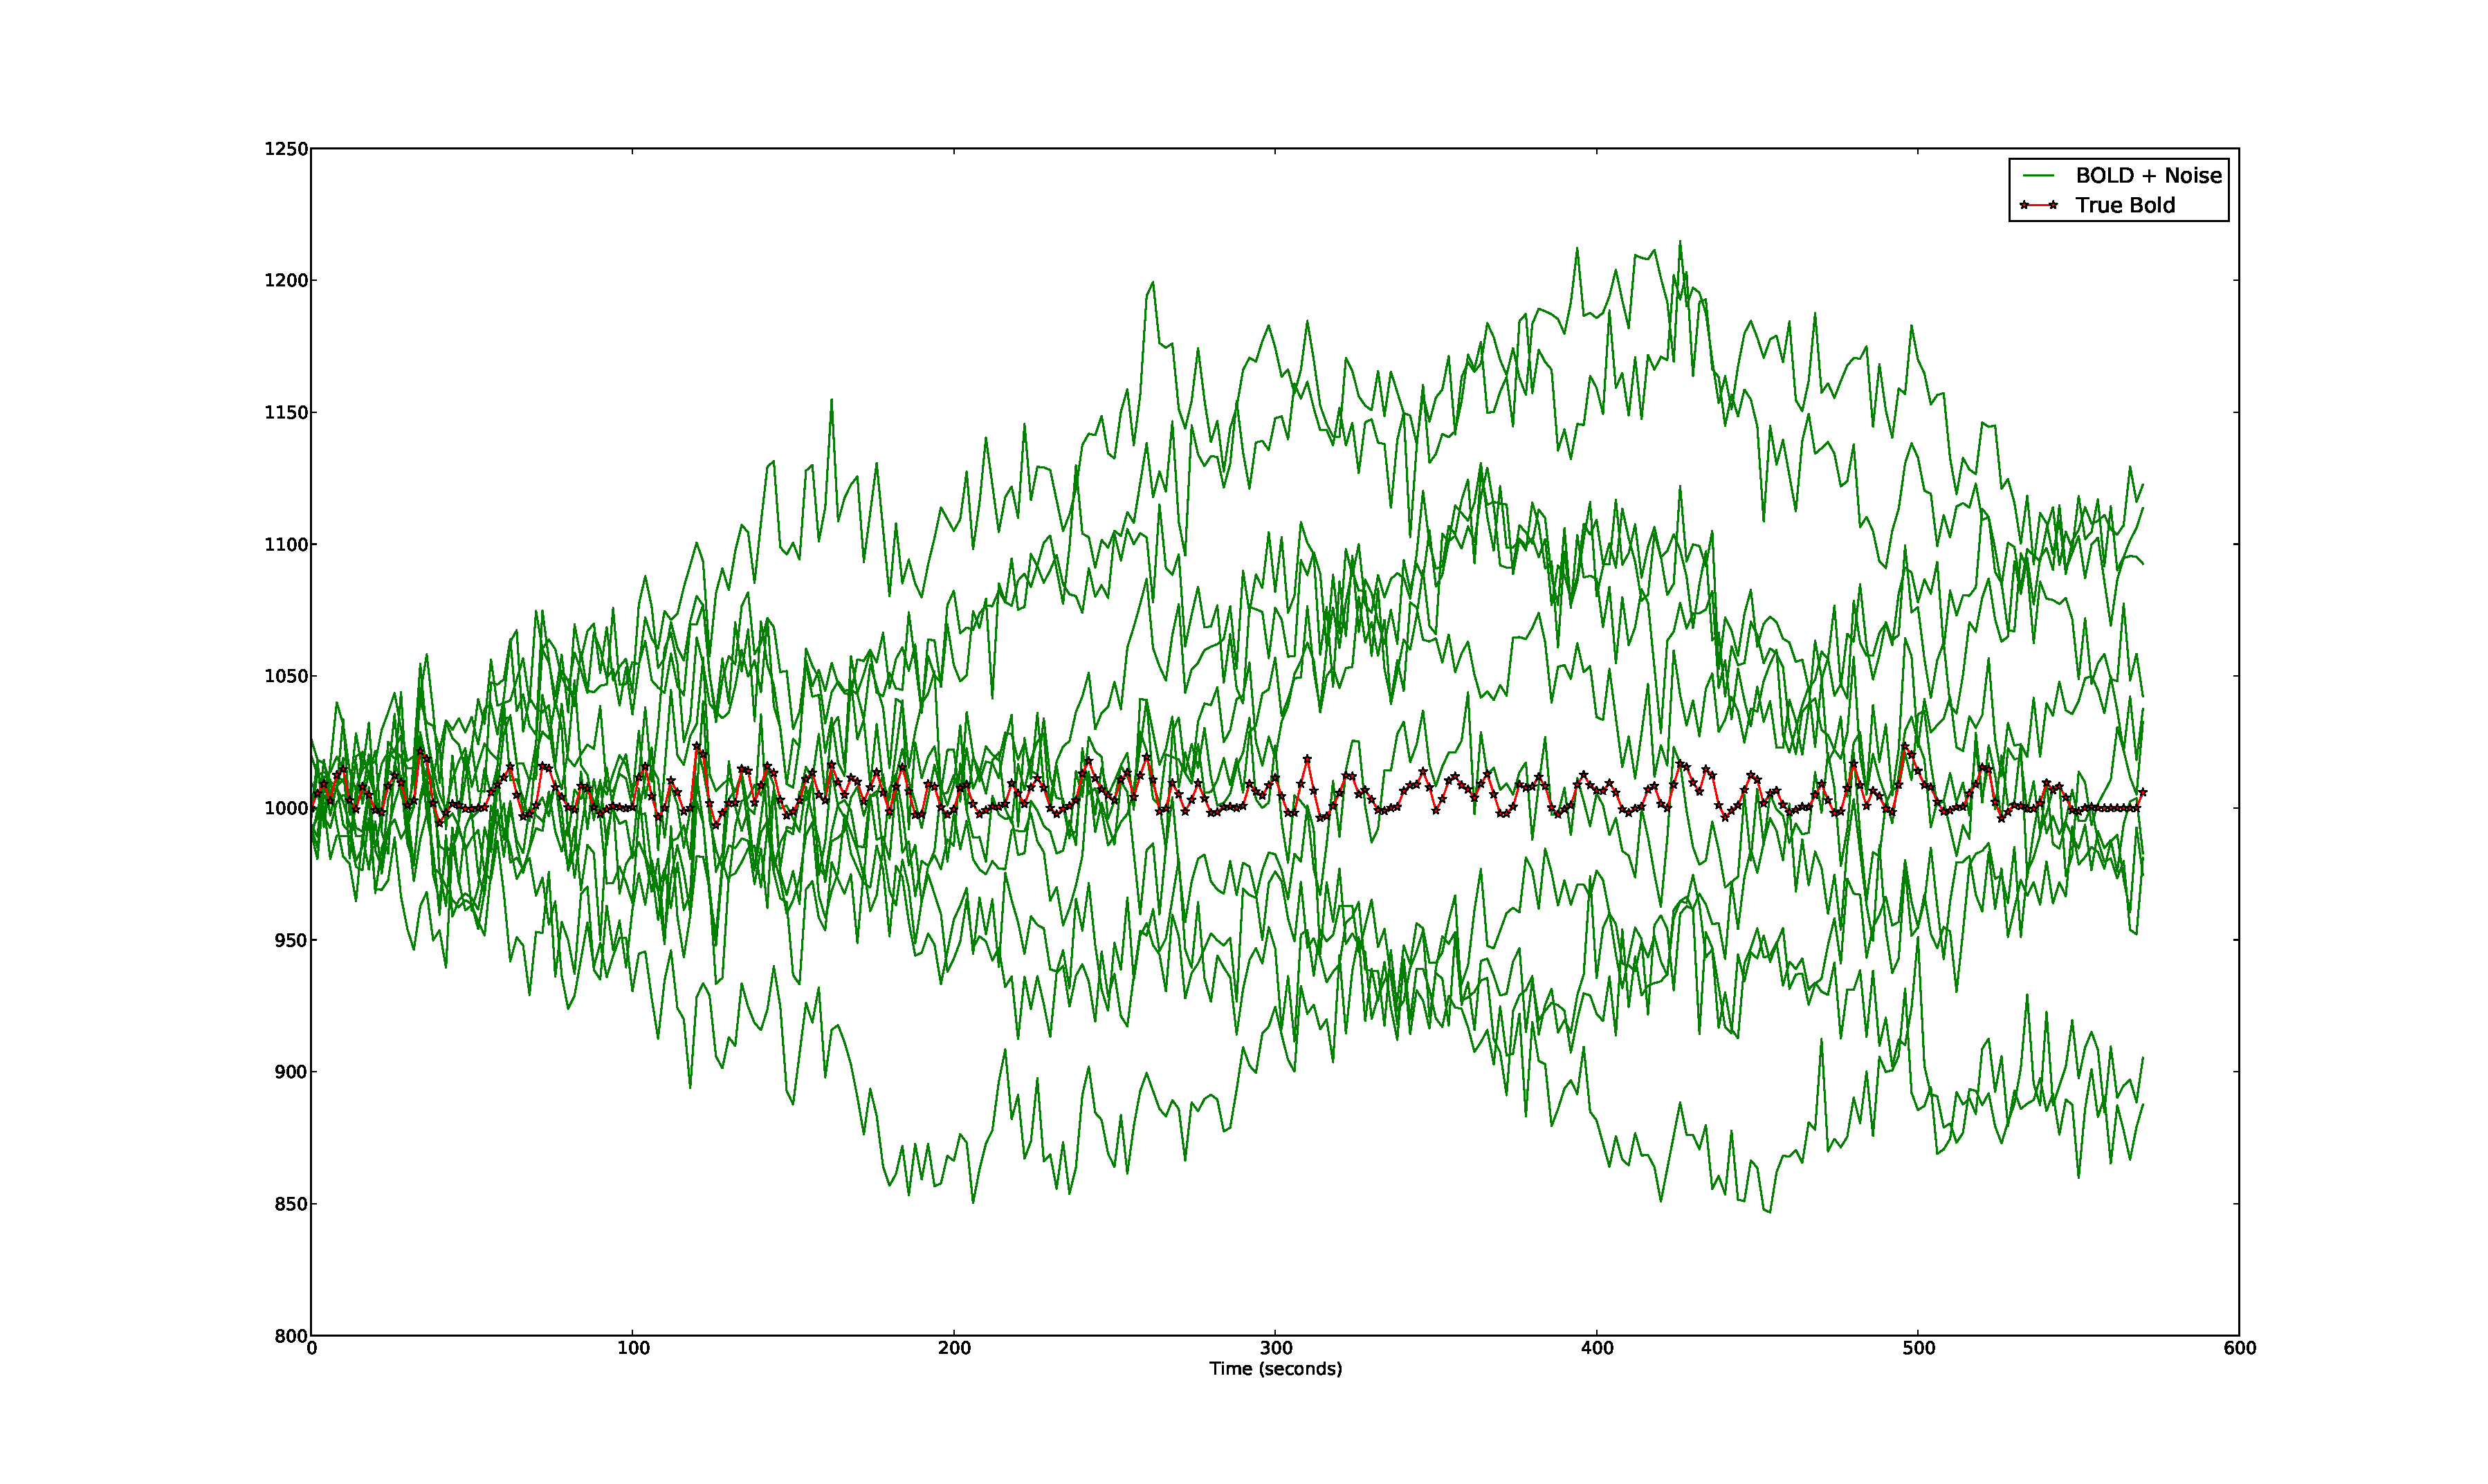
\includegraphics[trim=6cm 3cm 6cm 3cm,width=16cm]{images/realization_highnoise}
\caption{Test Signals with high noise compared to the clean signal, $\sigma_x = .01, \sigma_y=.005$}
\end{figure}
\begin{figure}[H]
\label{fig:PreprocessedHighNoise}
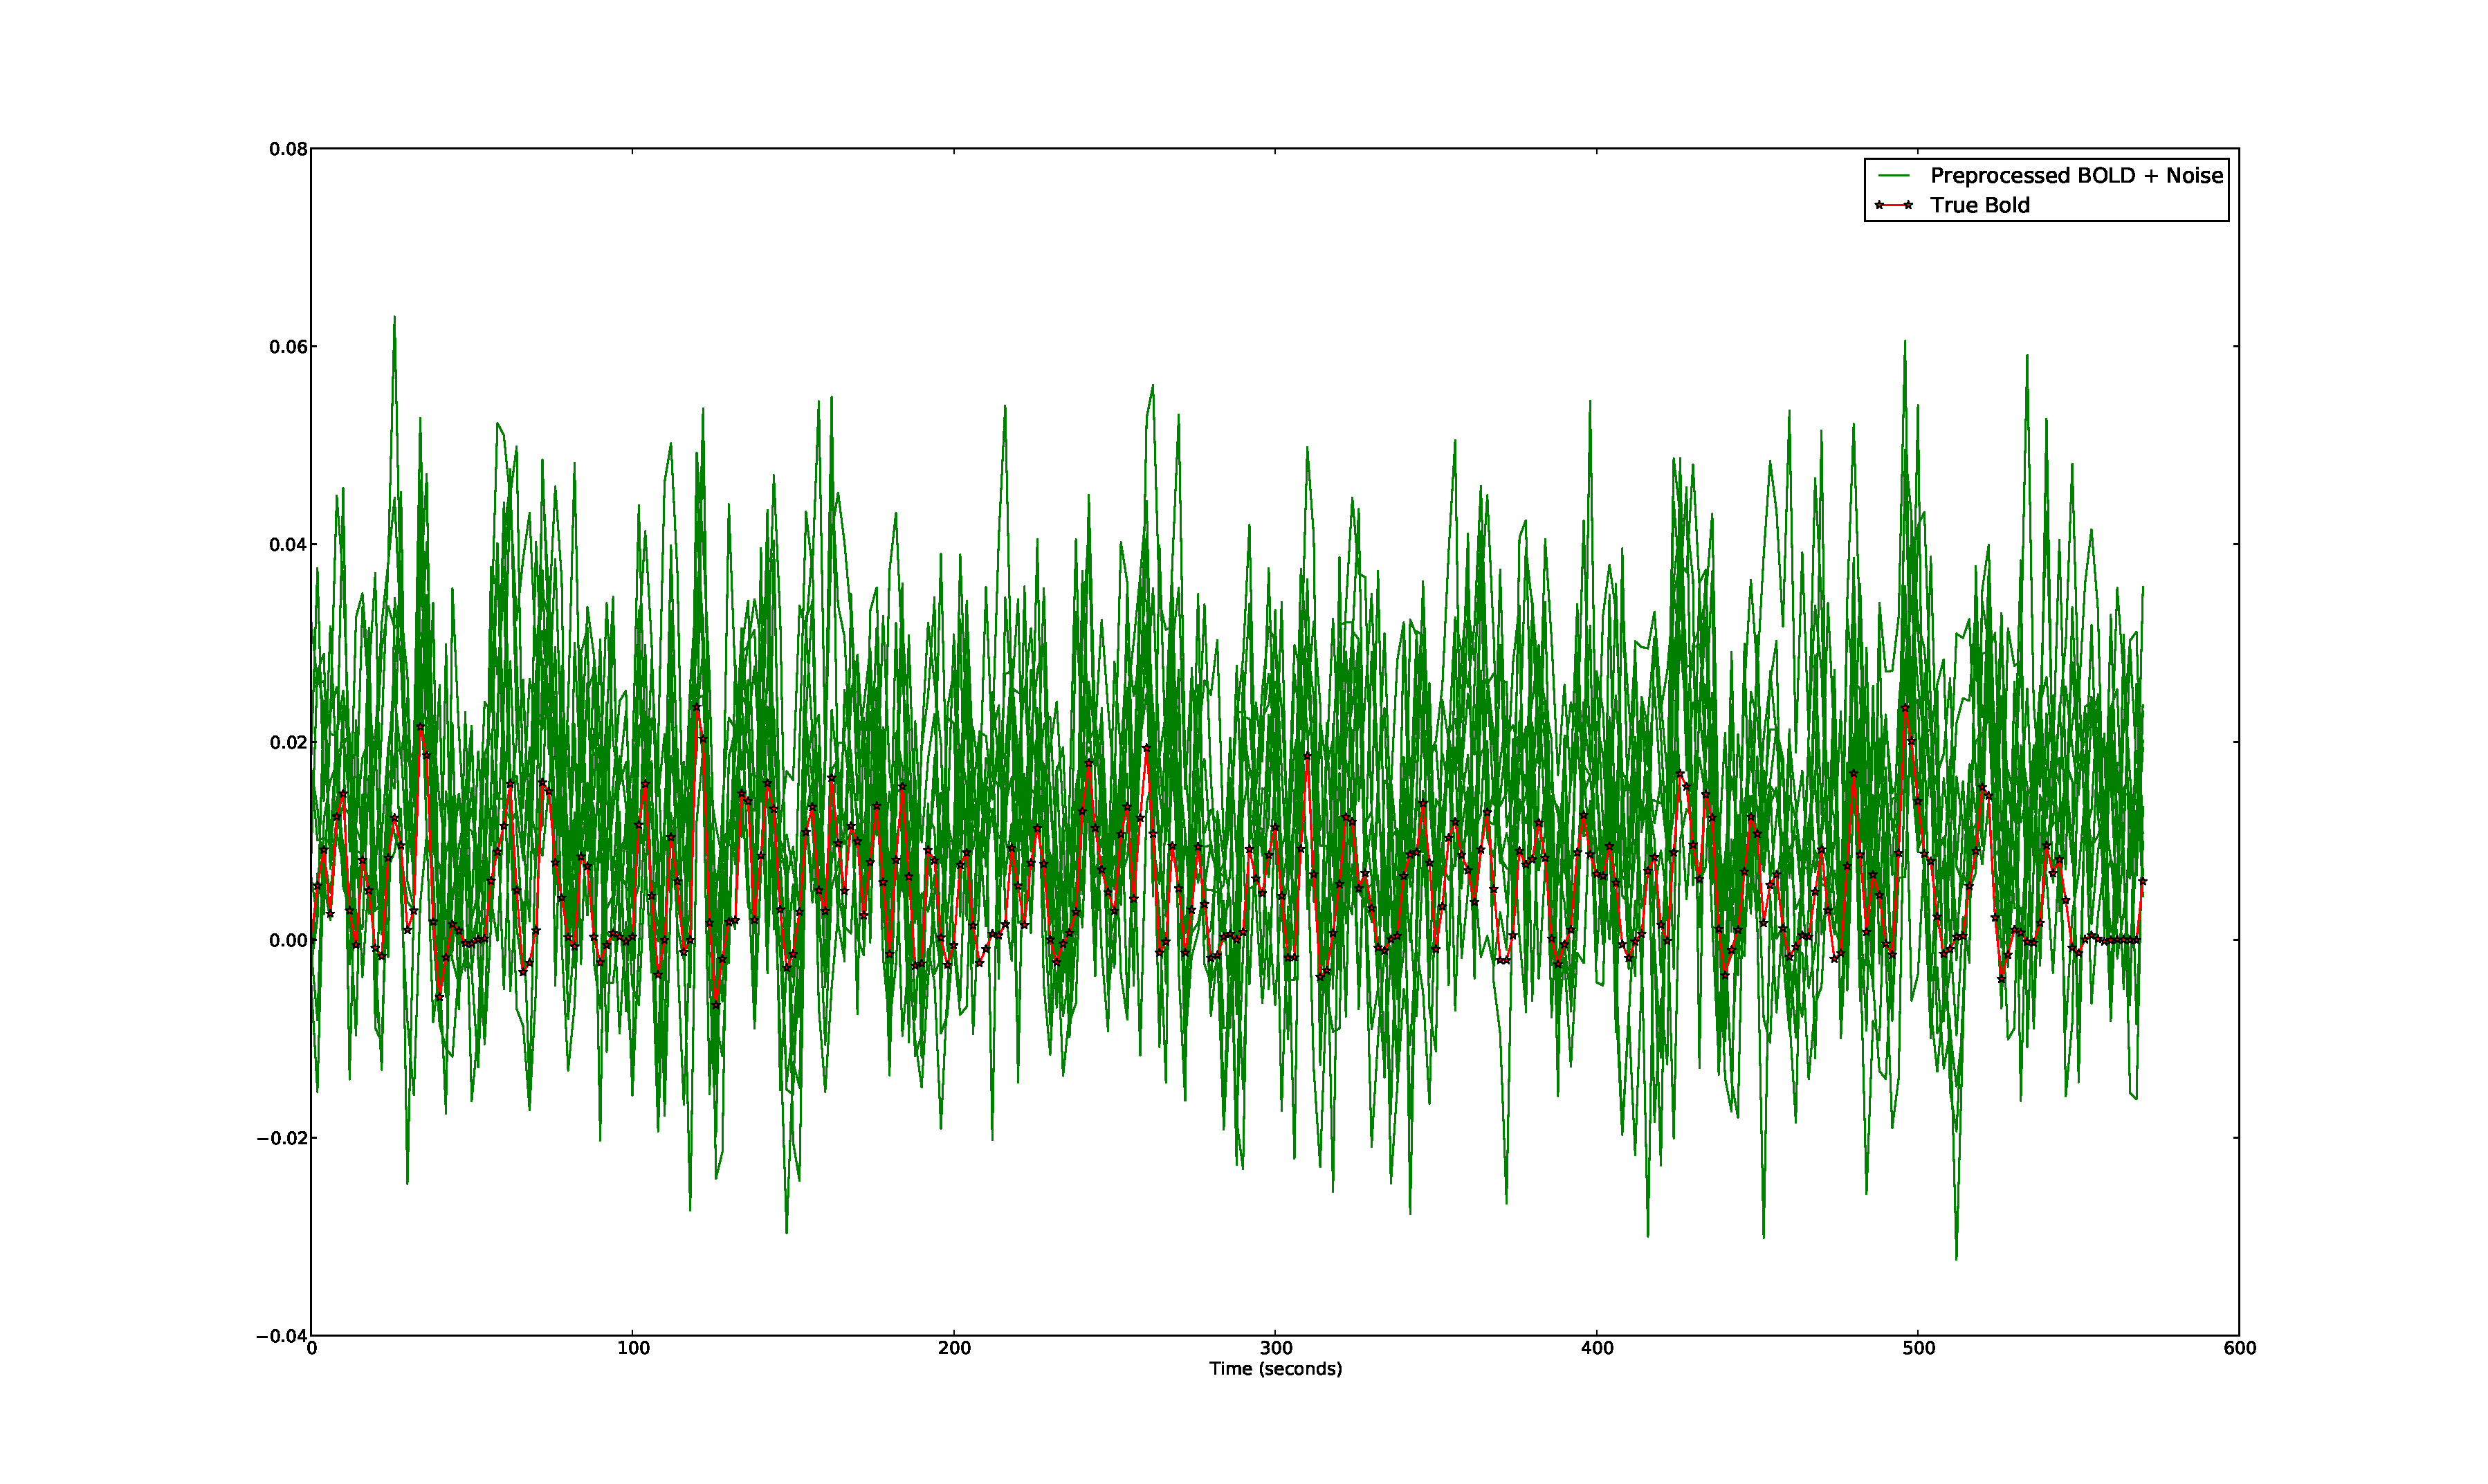
\includegraphics[trim=6cm 3cm 6cm 3cm,width=16cm]{images/preprocessed_highnoise}
\caption{A comparison of the preprocessed signals for the high noise case.}
\end{figure}

The results of the particle filter, for each of the ten runs may be seen in 
\autoref{fig:FitComparisonHighNoise}. Clearly the preprocessing led the algorithm
to somewhat higher activation levels, and it would appear that the subtleties of
different time constants are also lost for most of the runs, although a few seem
to manage quite accurate results. 

\begin{figure}[H]
\label{fig:FitComparisonHighNoise}
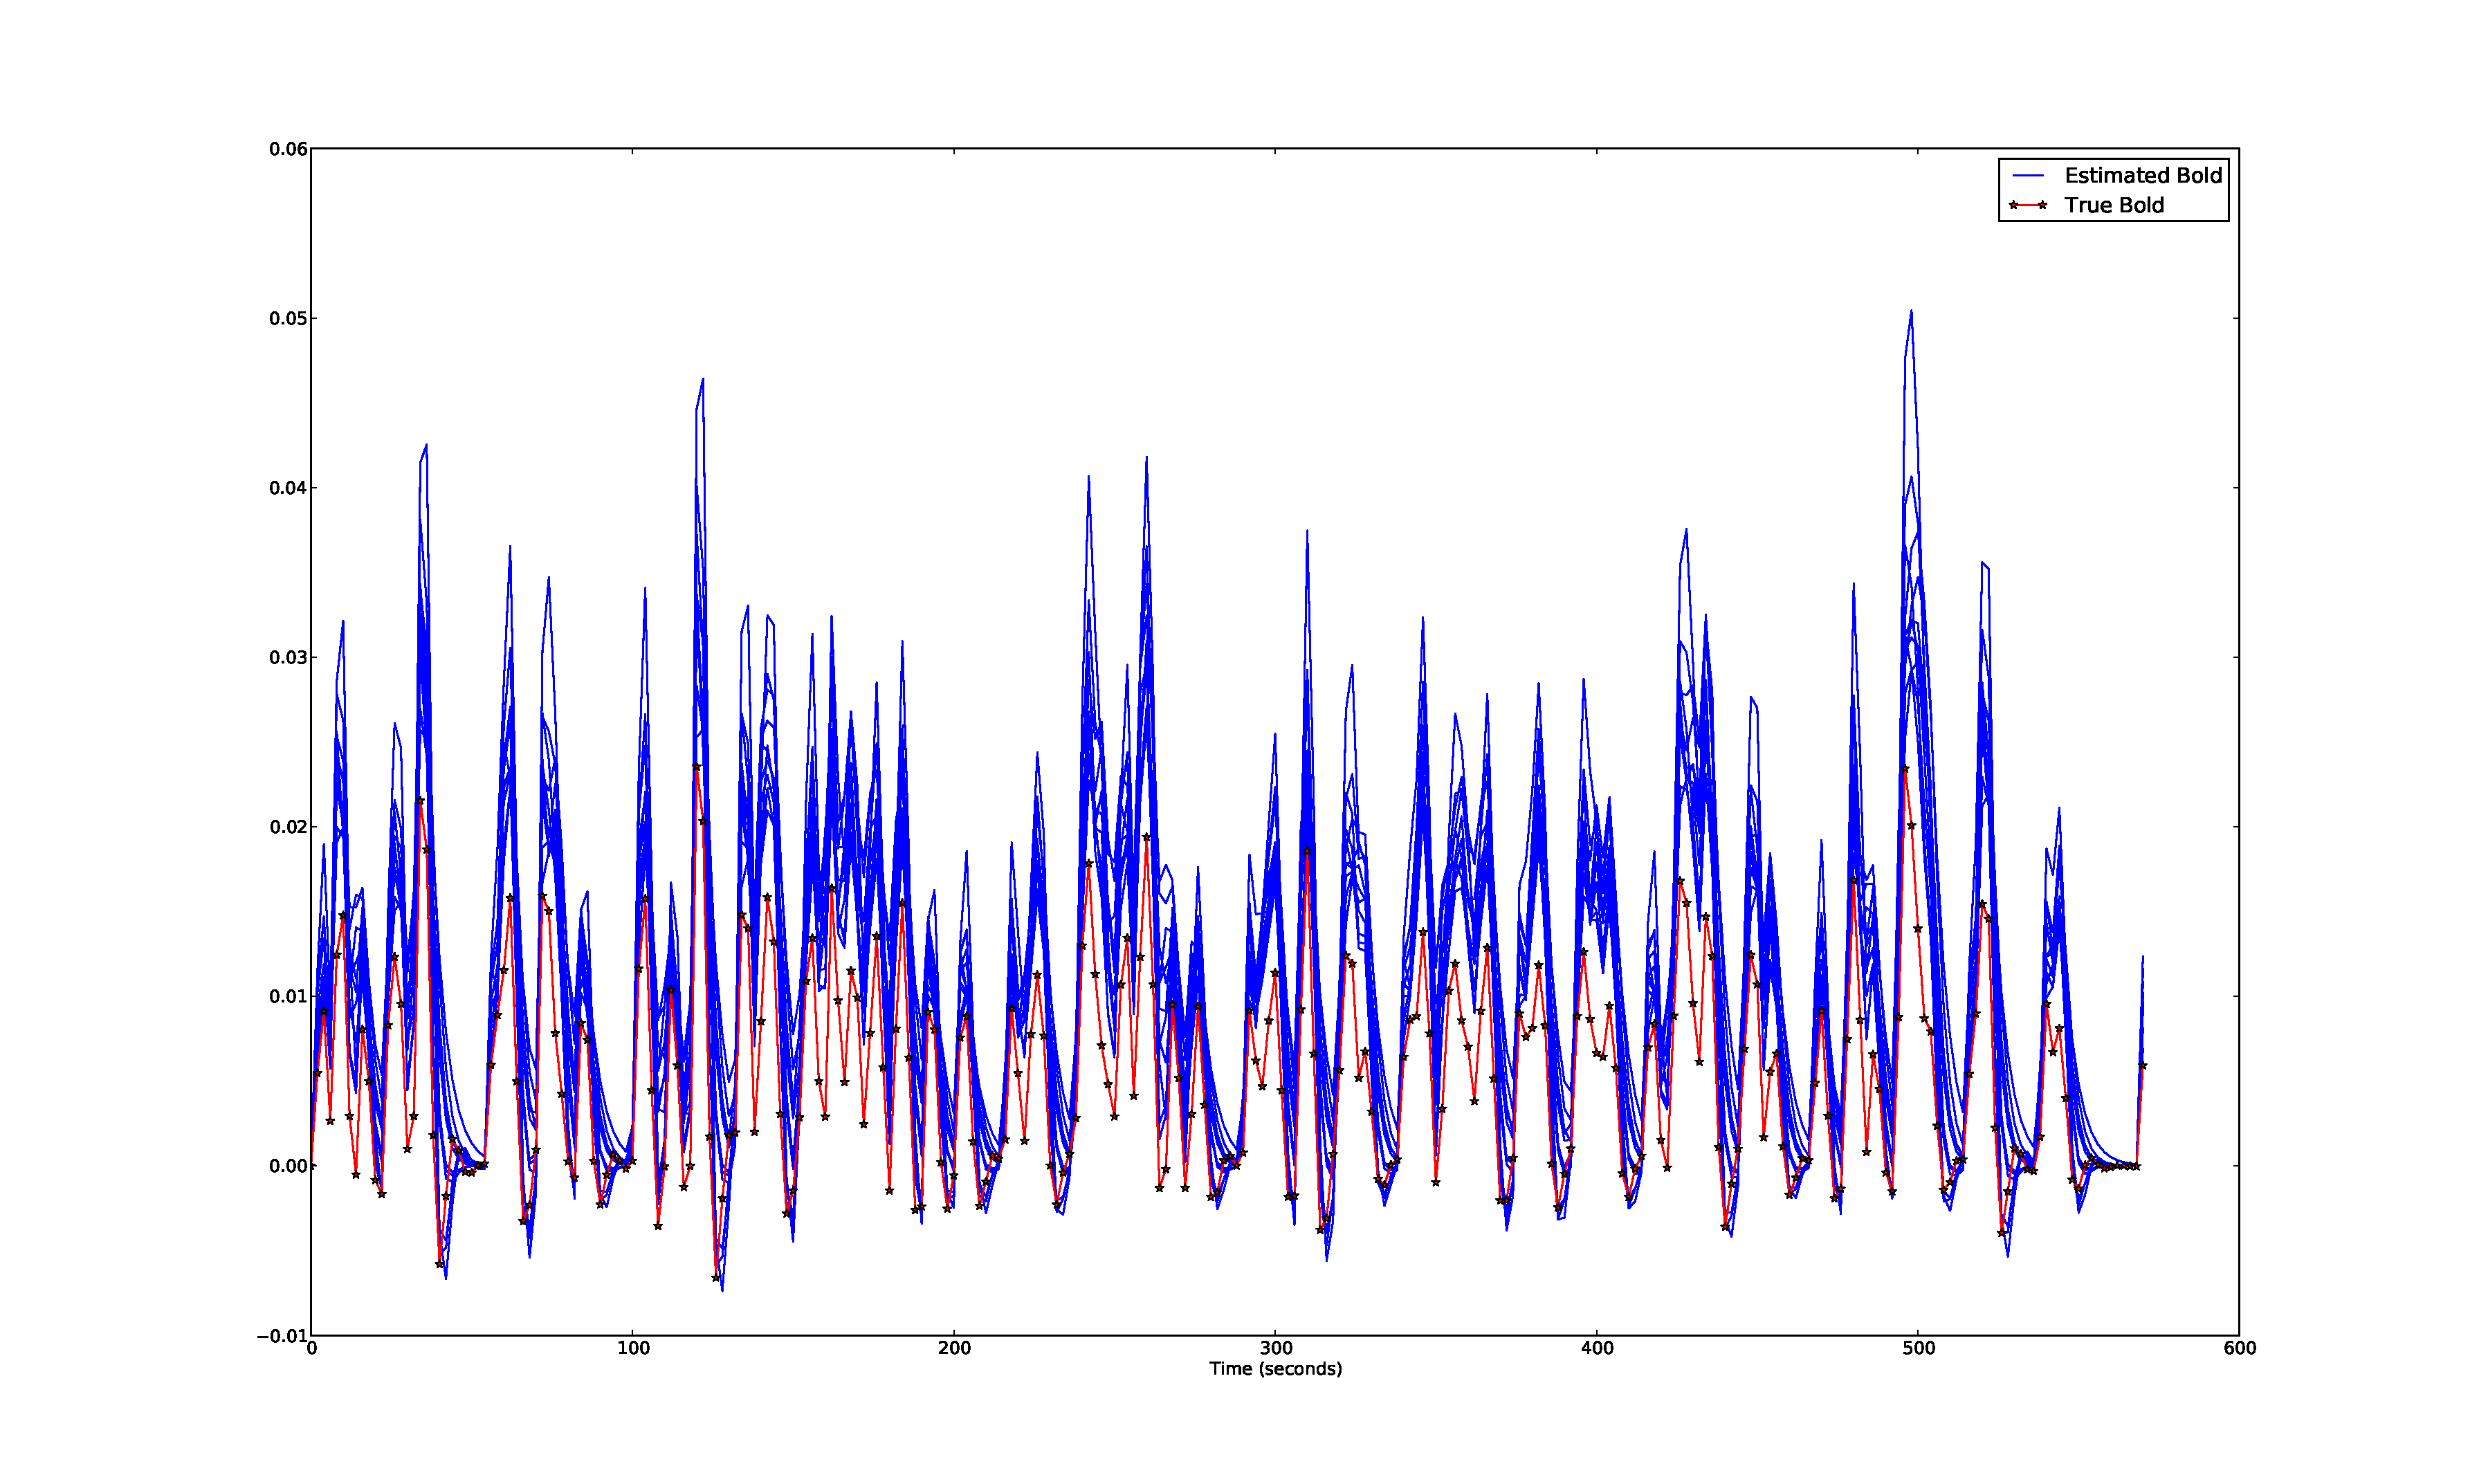
\includegraphics[trim=6cm 3cm 6cm 3cm,width=16cm]{images/comparison_highnoise}
\caption{A comparison of the fitted signals for the high noise case.}
\end{figure}
\begin{figure}[H]
\label{fig:NoiseComparisonJustTwo}
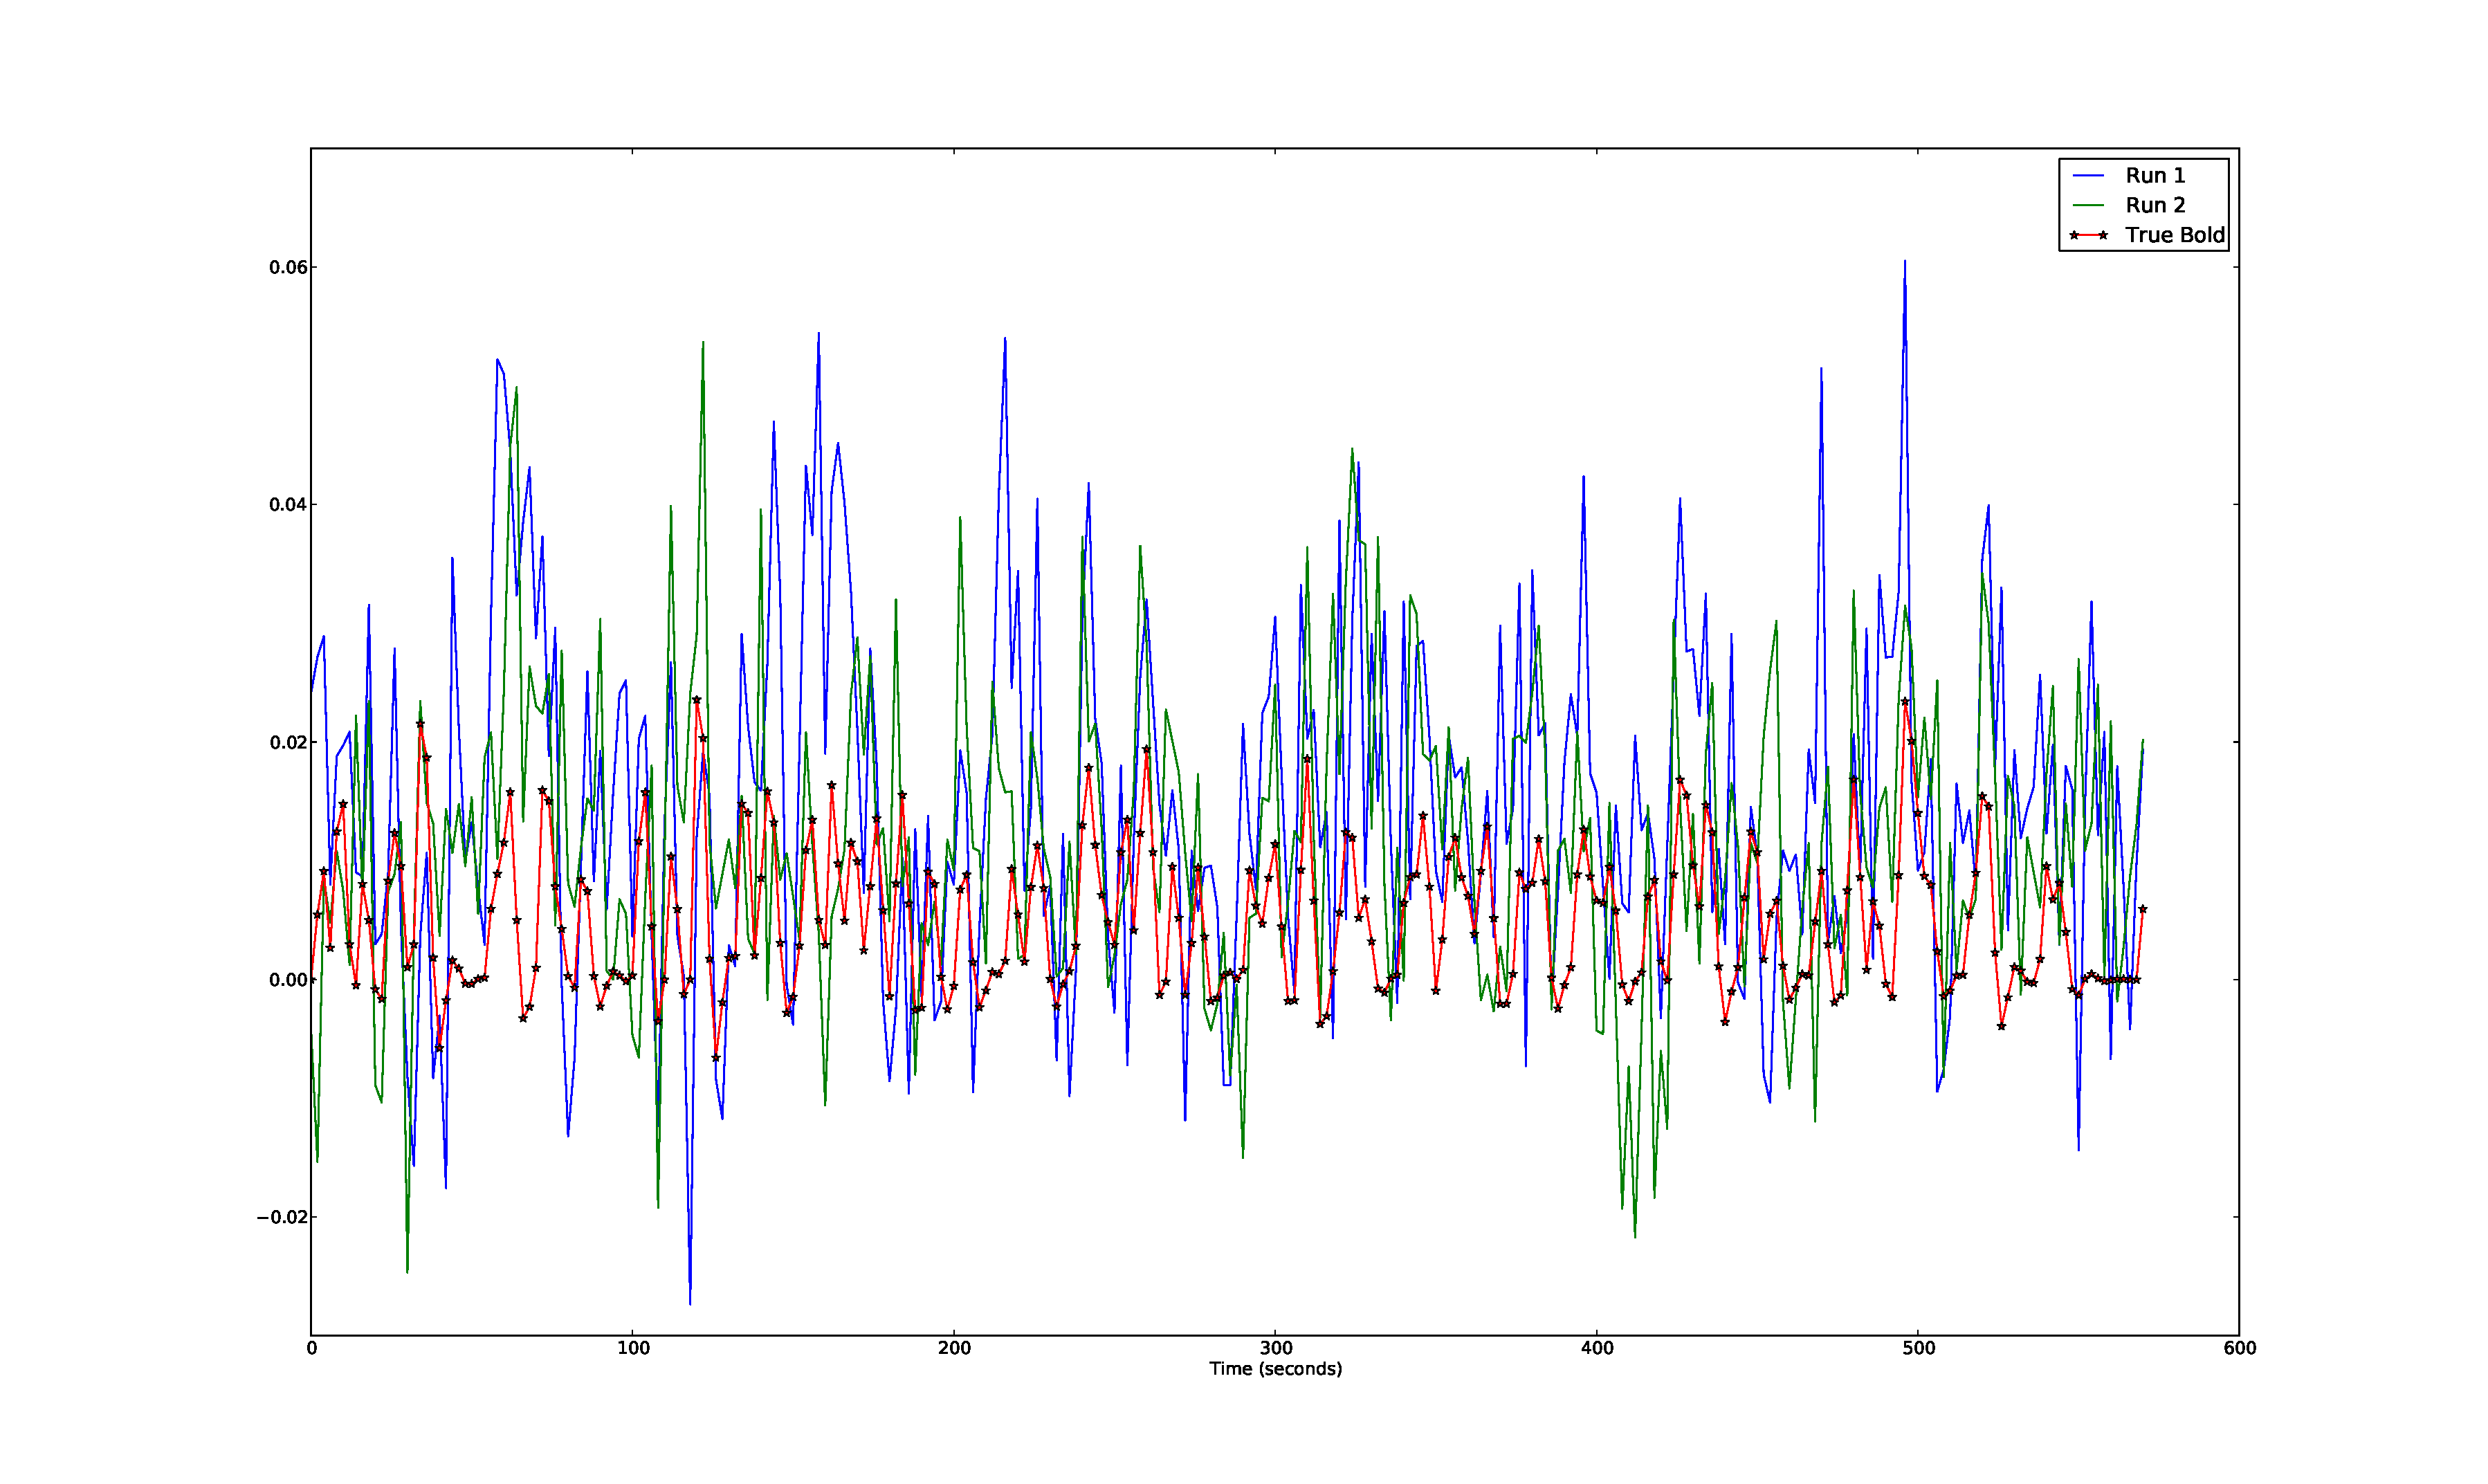
\includegraphics[trim=6cm 3cm 6cm 3cm,width=16cm]{images/highnoise_56_noise}
\caption{Two particular preprocessed noise realizations for the high noise case.}
\end{figure}
\begin{figure}[H]
\label{fig:FitComparisonHighNoiseJust2}
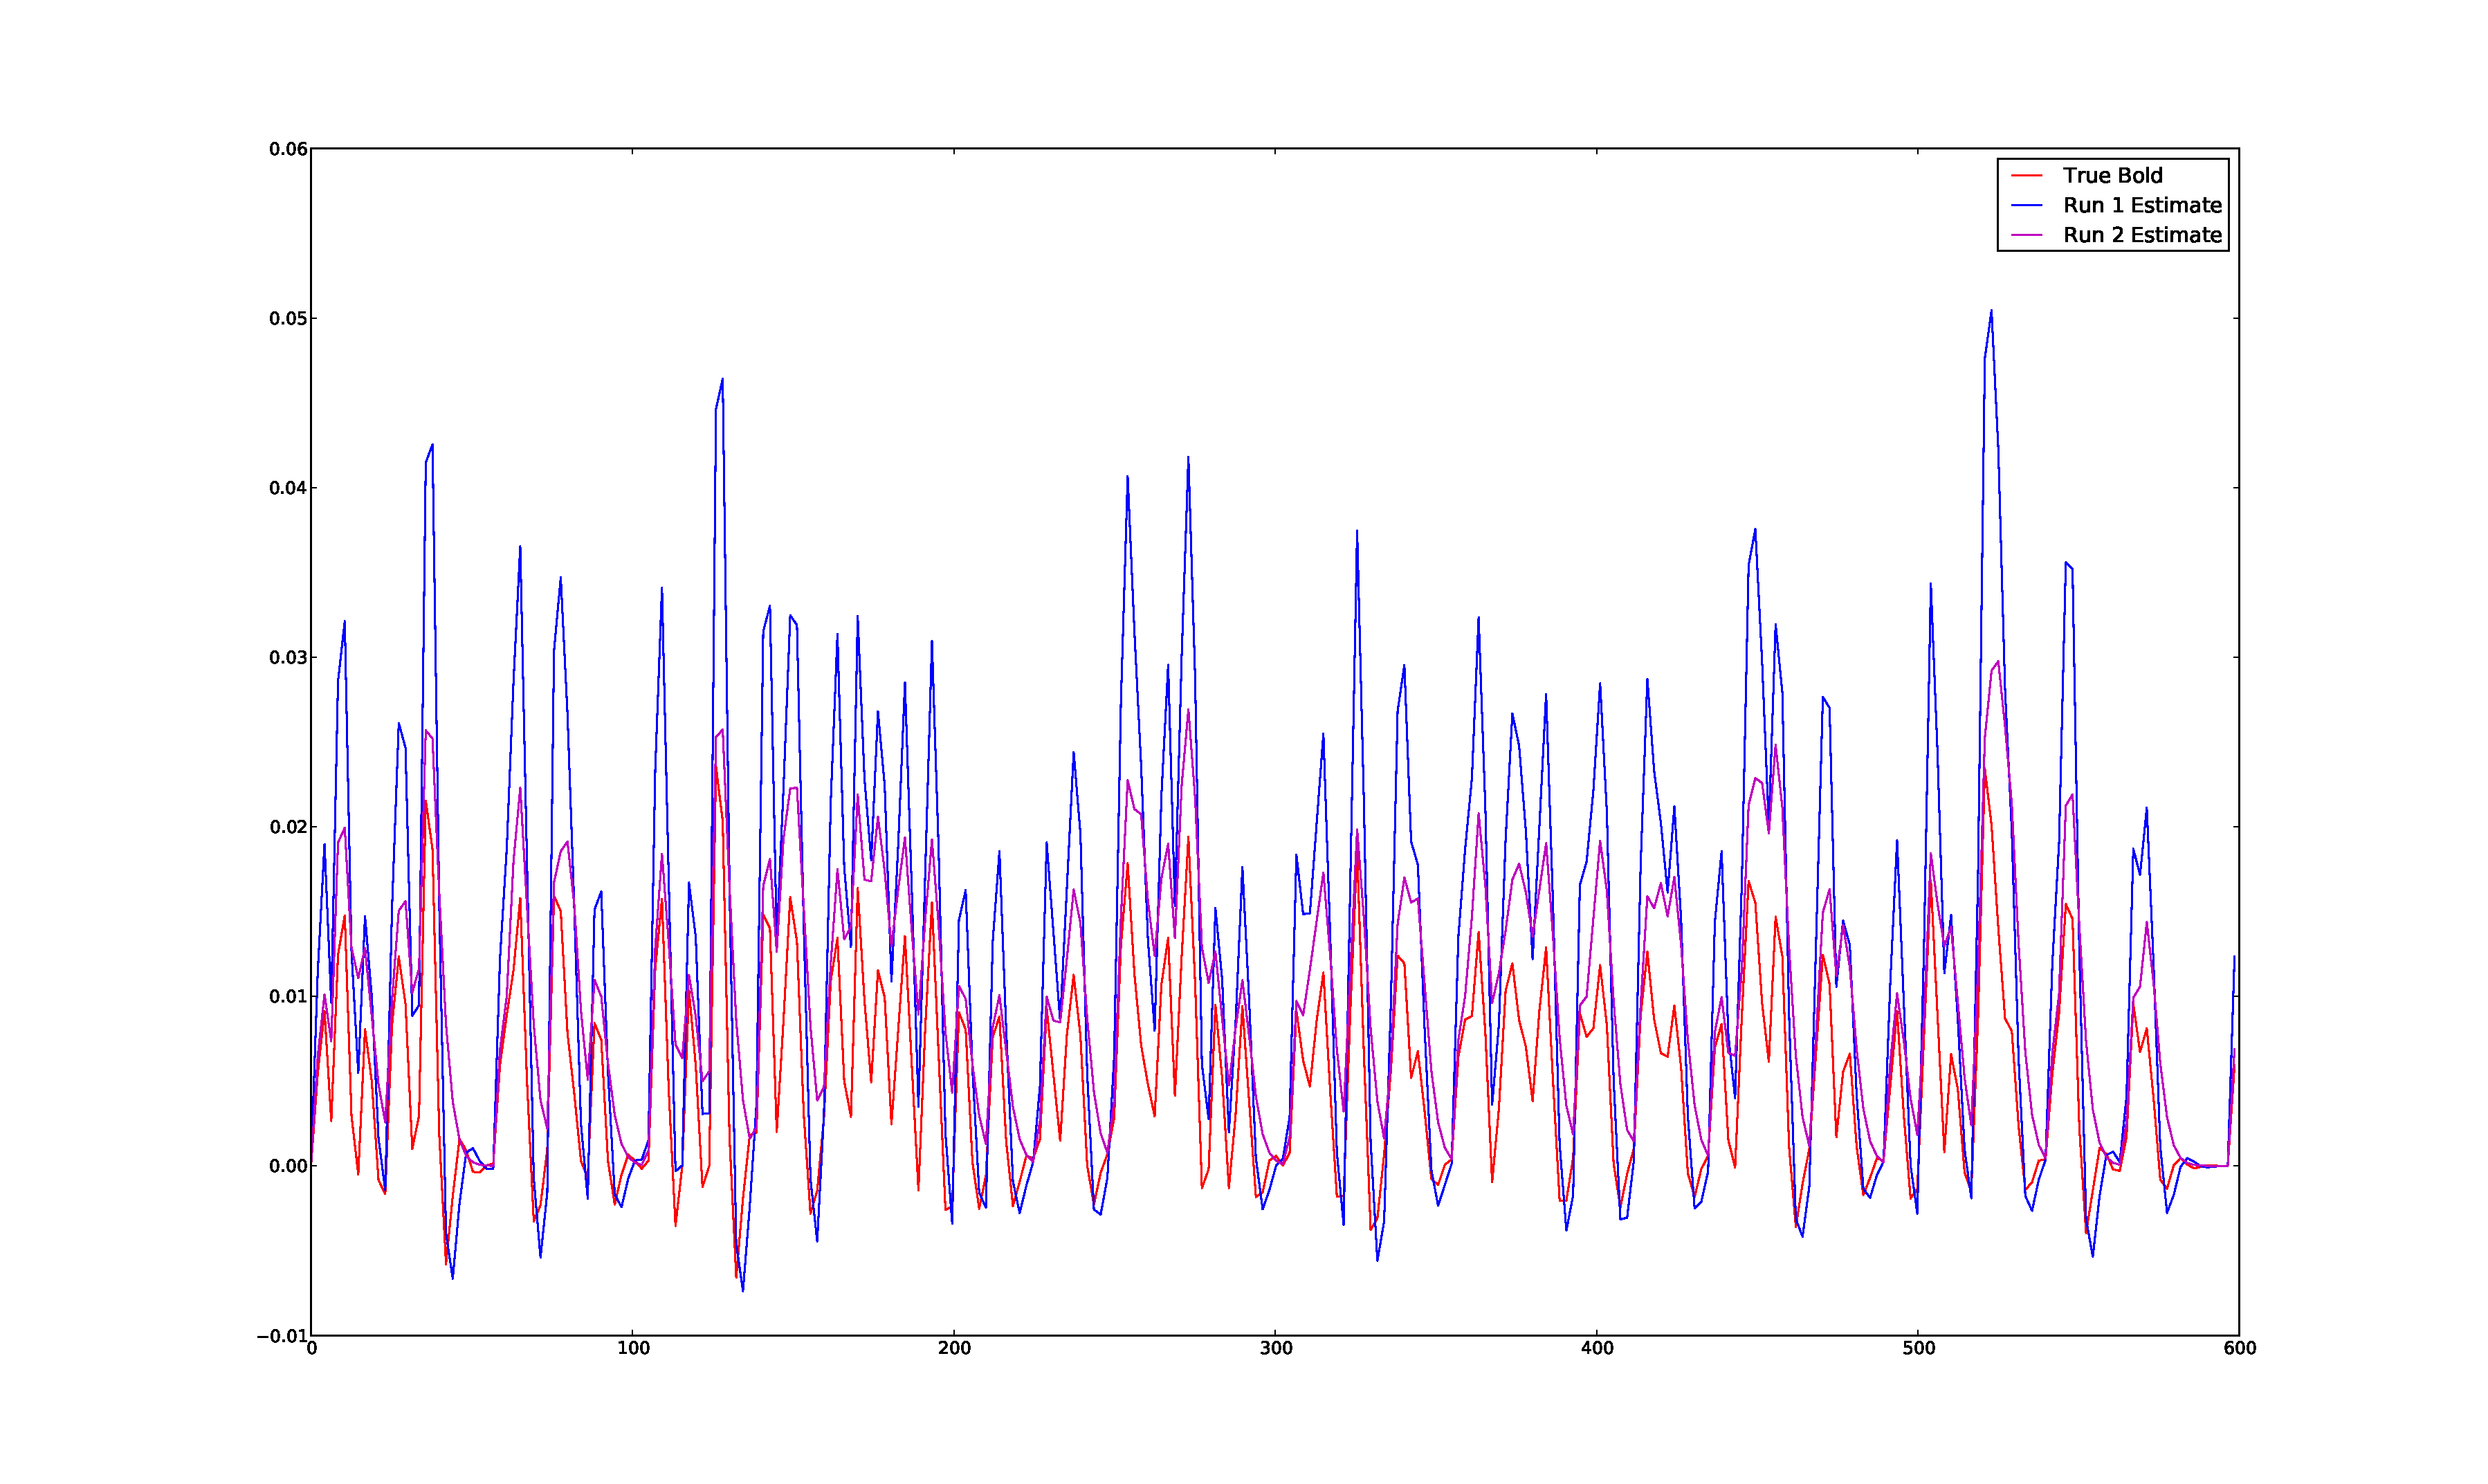
\includegraphics[trim=6cm 3cm 6cm 3cm,width=16cm]{images/comparison_highnoise_just2}
\caption{The results for the noise realizations shown in \autoref{fig:NoiseComparisonJustTwo}.}
\end{figure}

It is interesting to consider how the preprocessing and noise may effect the
parameters of the fitting model. For instance run 1 in \autoref{fig:NoiseComparisonJustTwo}
certainly seems to be more biased toward higher peaks than run 2. There also appears
to be more drift than the 20 points per knot could fit, which explains the 
prolonged increase at 170 seconds. Despite run 1's bias toward higher peaks, for
some reason the particle filter was able to get a much better match for the
modeled post-stimulus undershoot (which is likely significantly shorter than it
should be). Ultimately the results are pretty good. \autoref{tab:SimMSE} shows
the mean squared error for all two runs, and highlights the two runs analyzed here and 
in \autoref{fig:ConvergenceRuns1} and \autoref{fig:ConvergenceRuns2}.

\begin{figure}[H]
\subfigure[$\tau_0$, $\alpha$, $E_0$, $V_0$]
{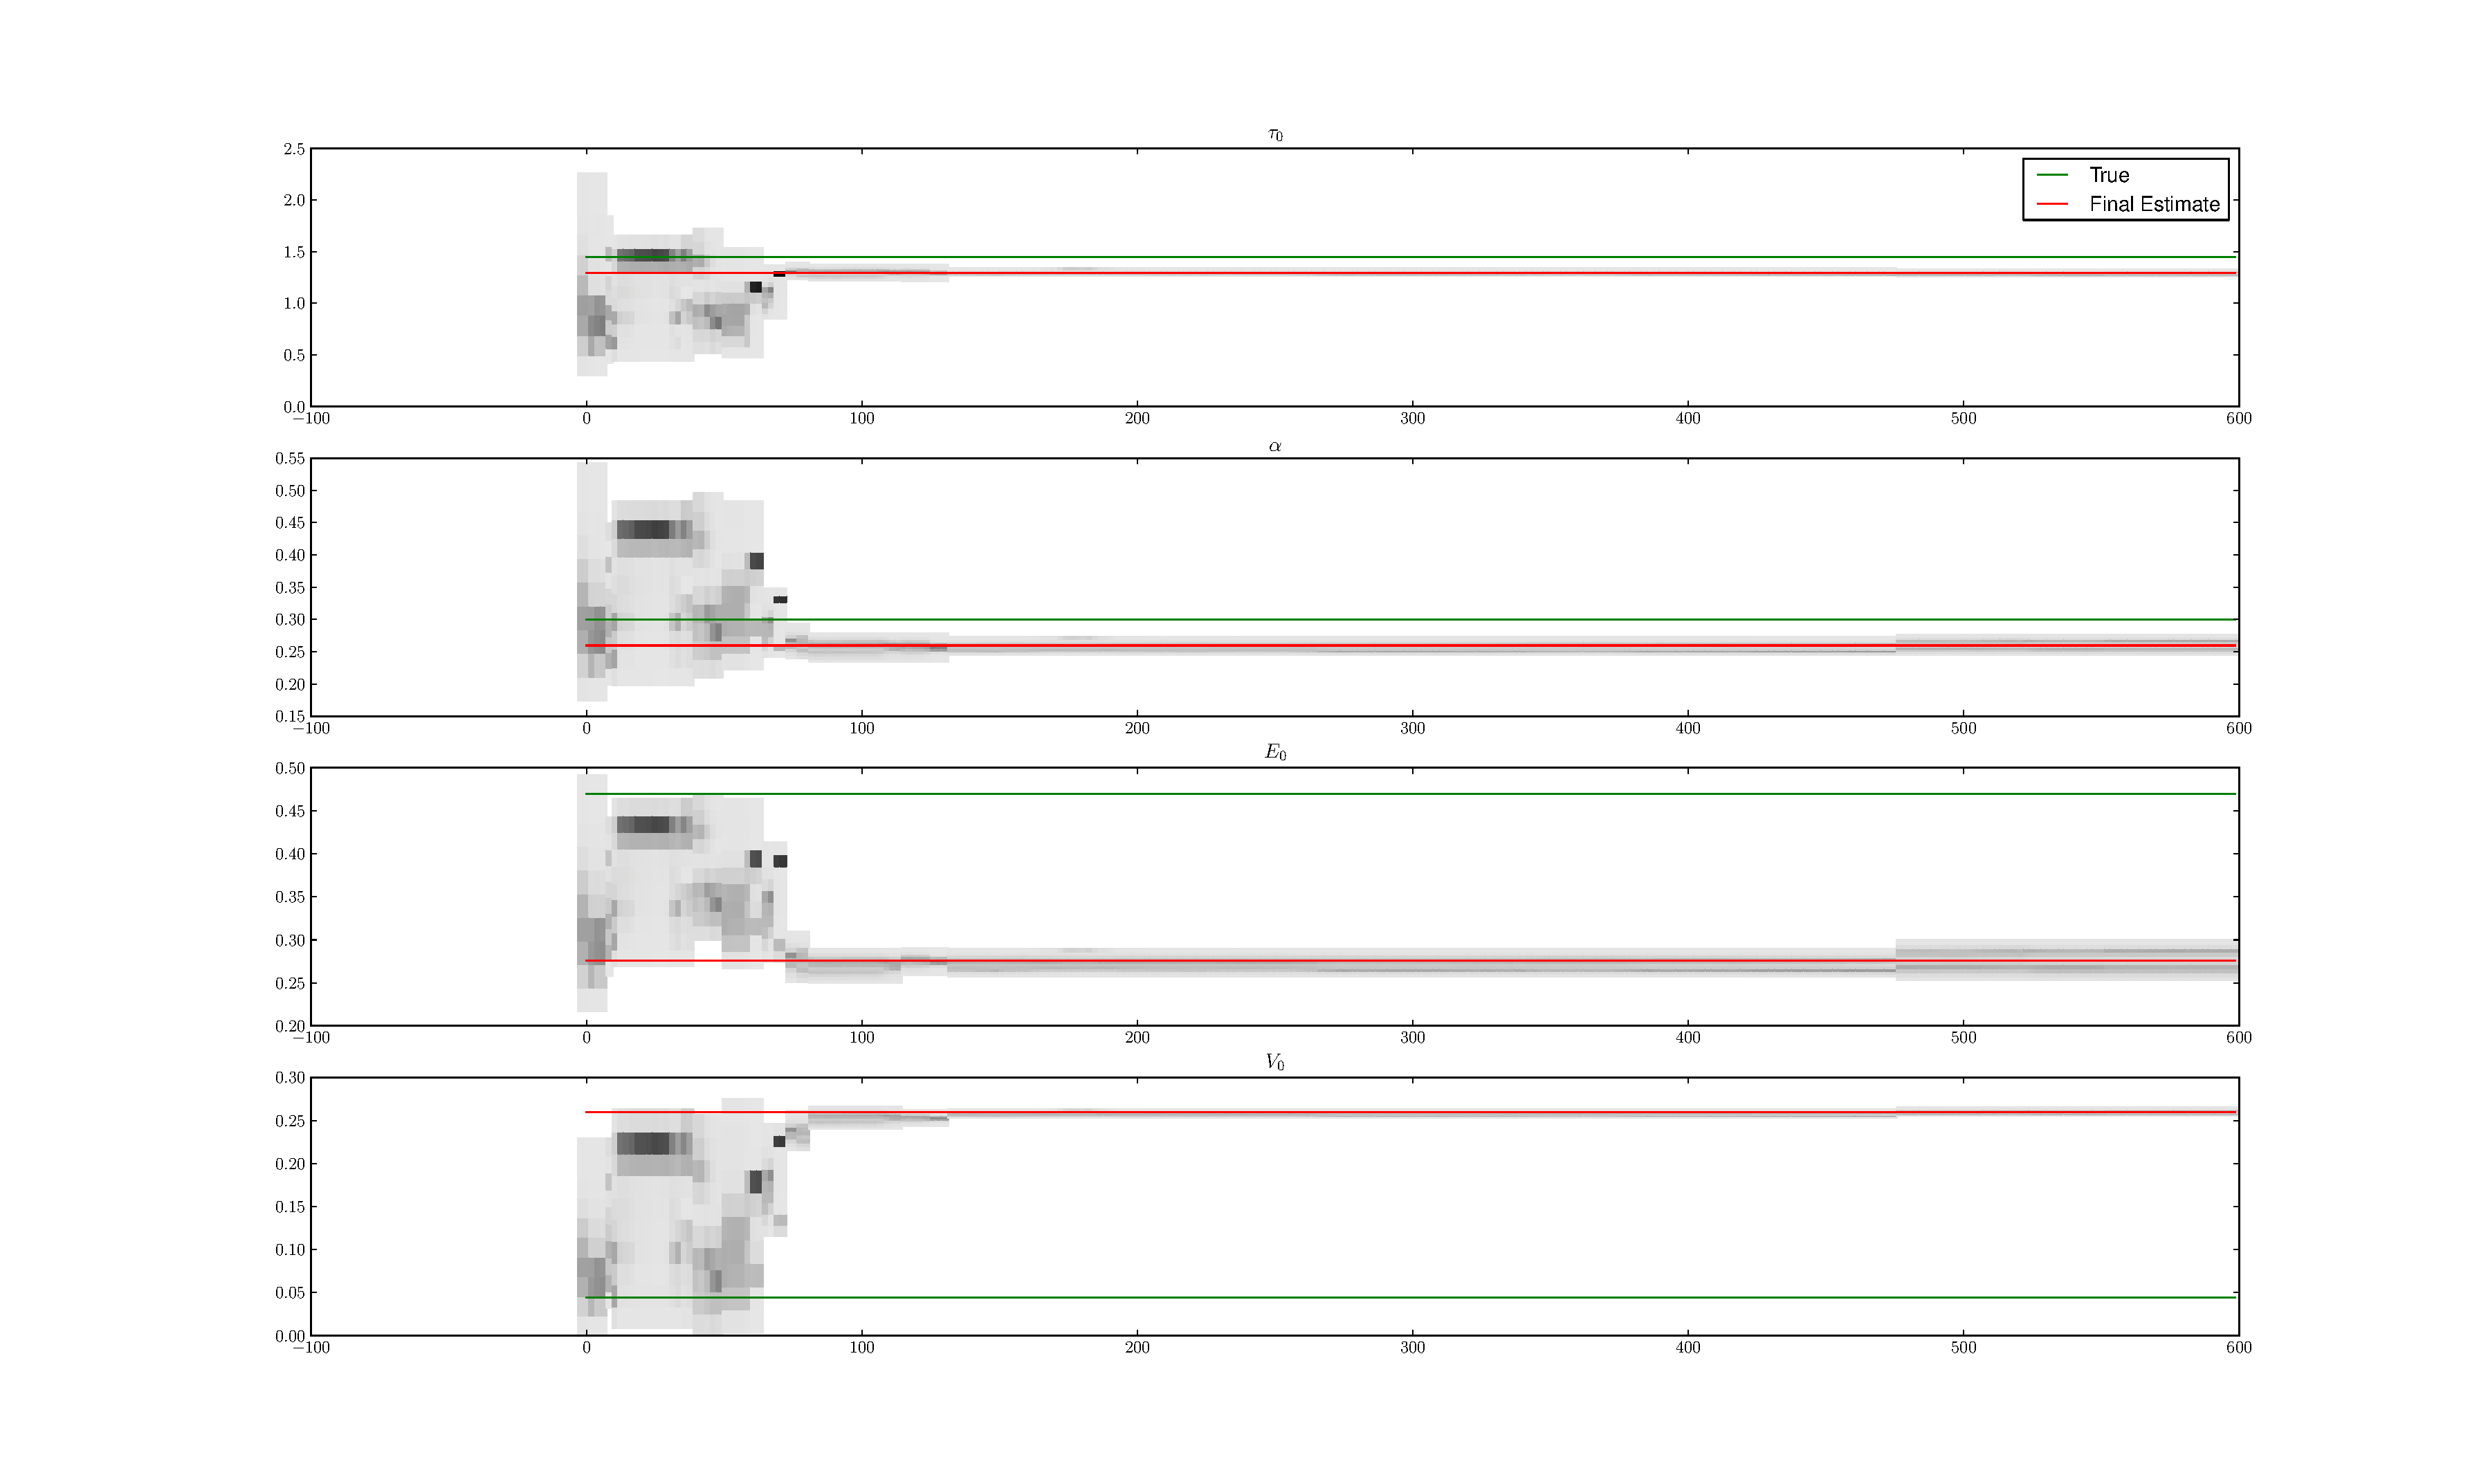
\includegraphics[trim=7cm 3cm 7cm 4cm, width=15cm]{images/highnoise_run5_1}}\\
\end{figure}
\begin{figure}[H]
\subfigure[$\tau_s$, $\tau_f$, $\epsilon$, $V$] 
{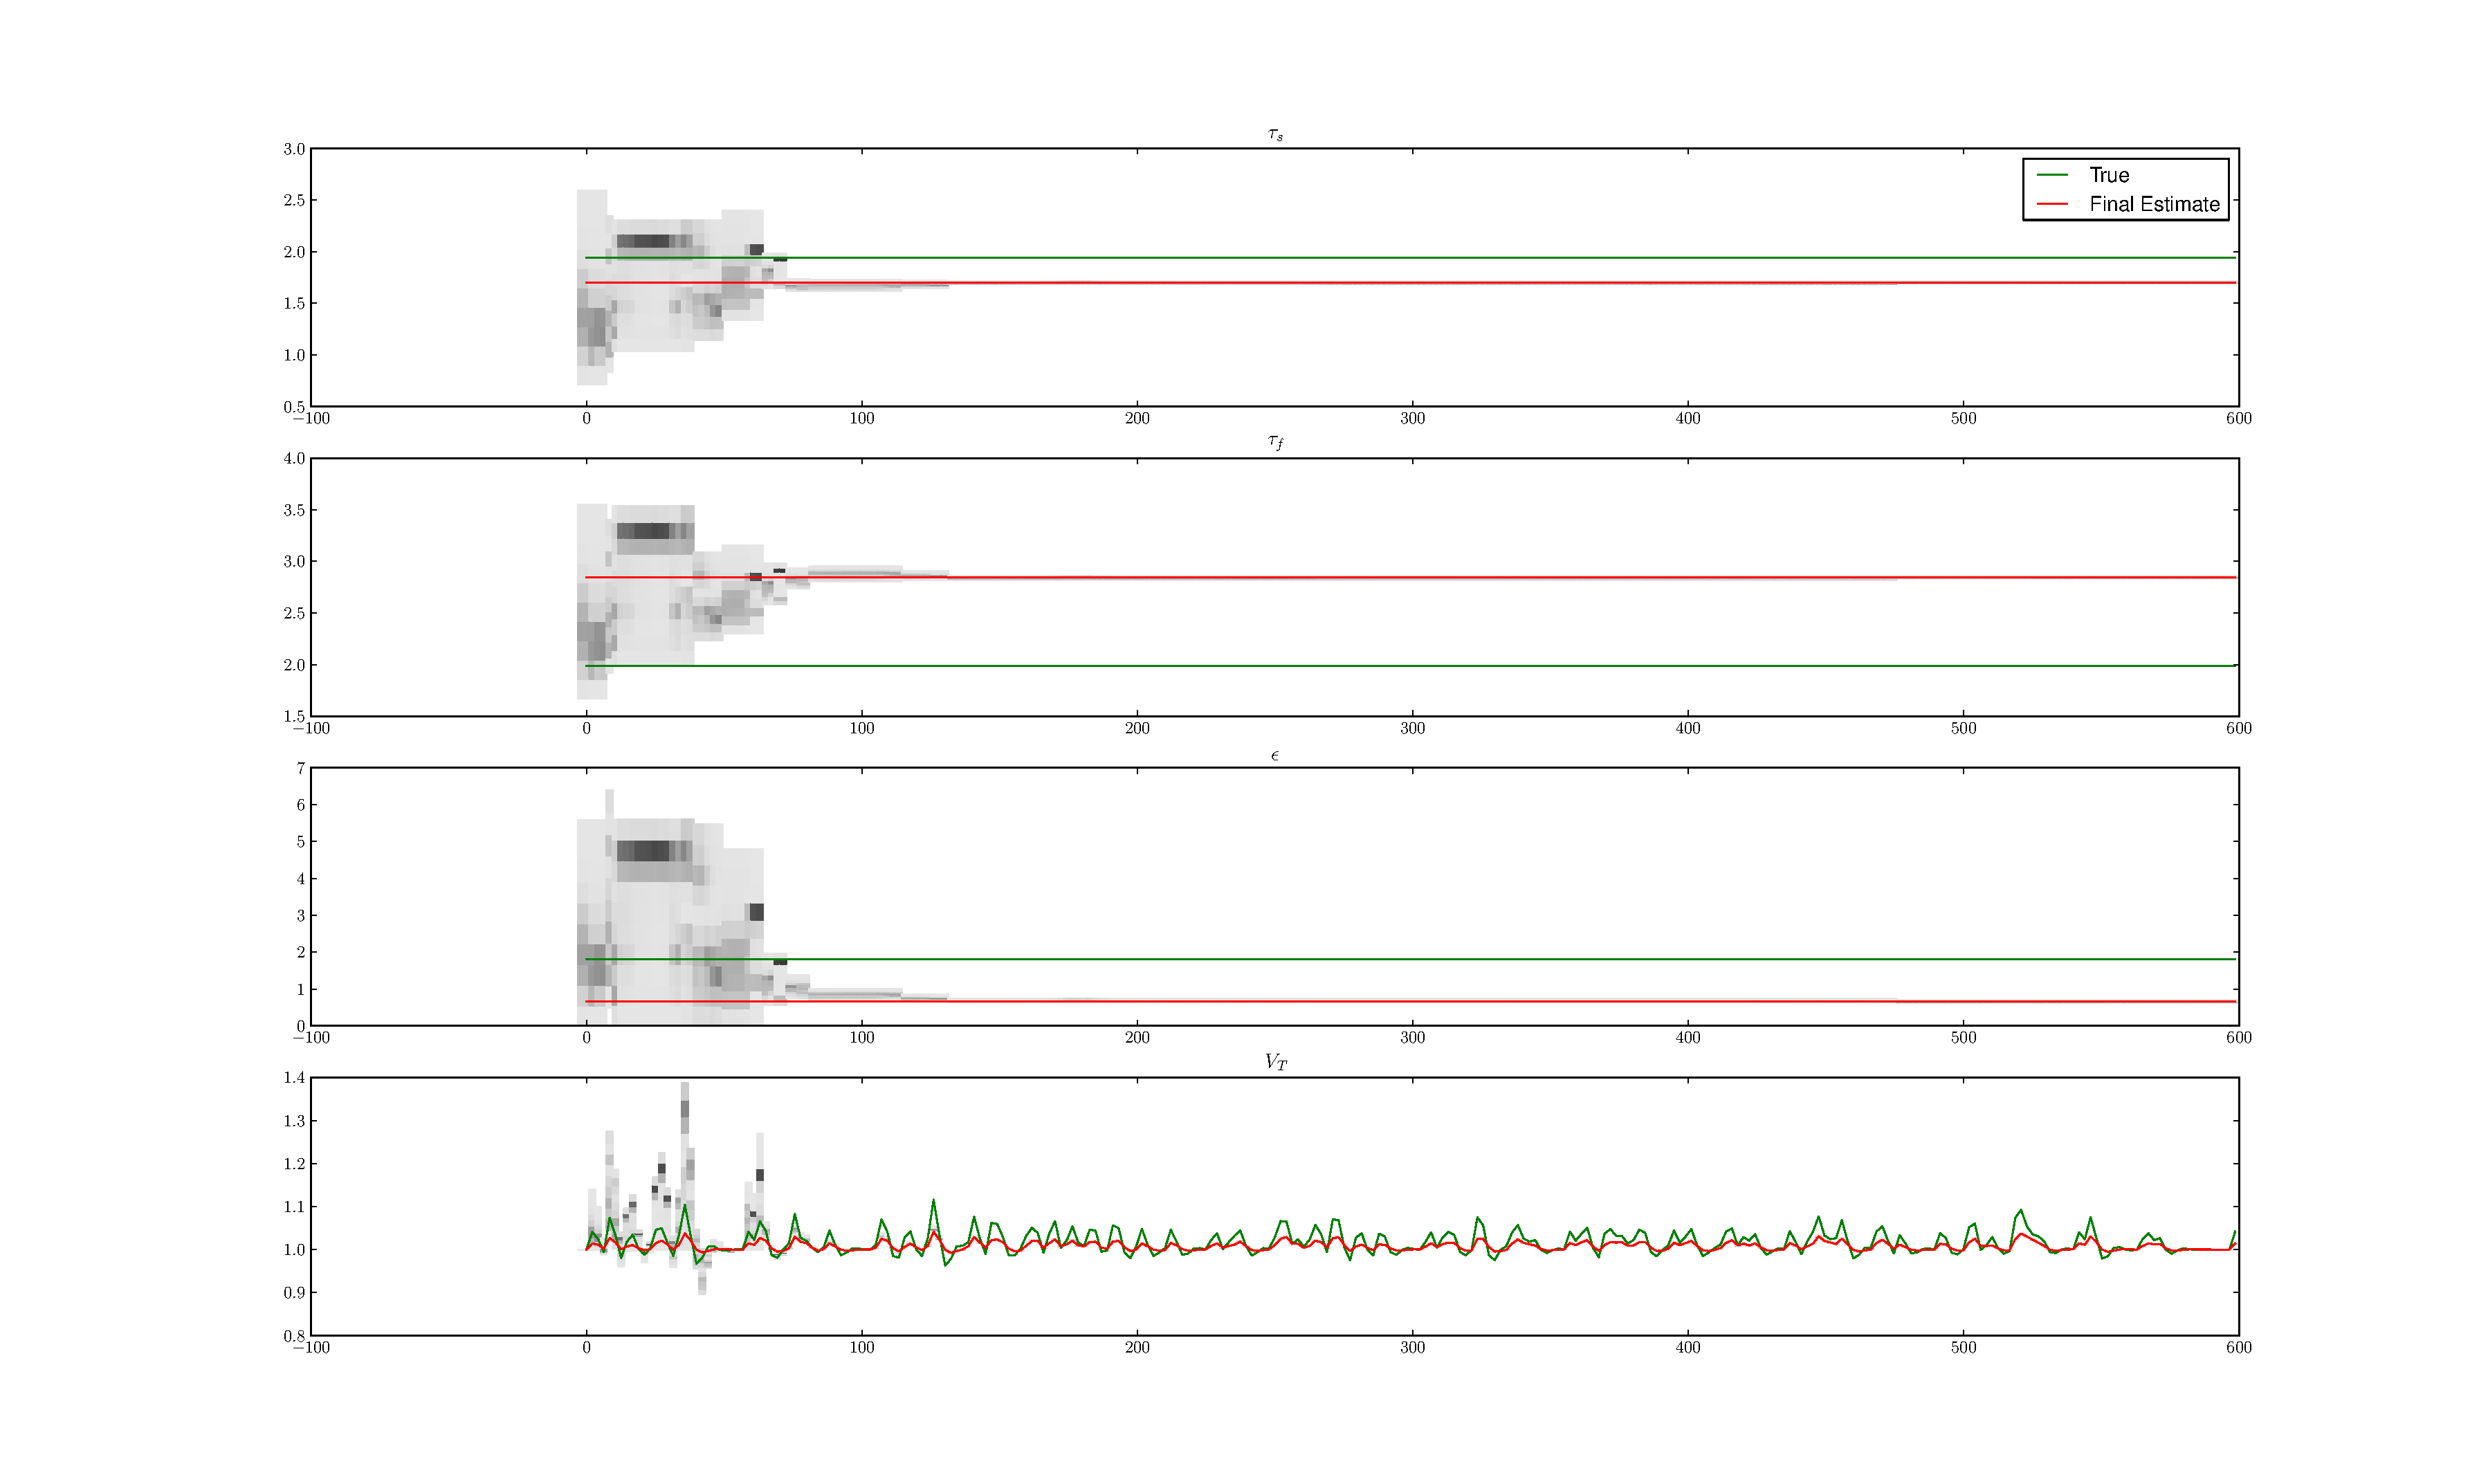
\includegraphics[trim=7cm 3cm 7cm 1cm, width=15cm]{images/highnoise_run5_2}}\\
\end{figure}
\begin{figure}[H]
\subfigure[$Q$, $S$, $F$, $BOLD$ ]
{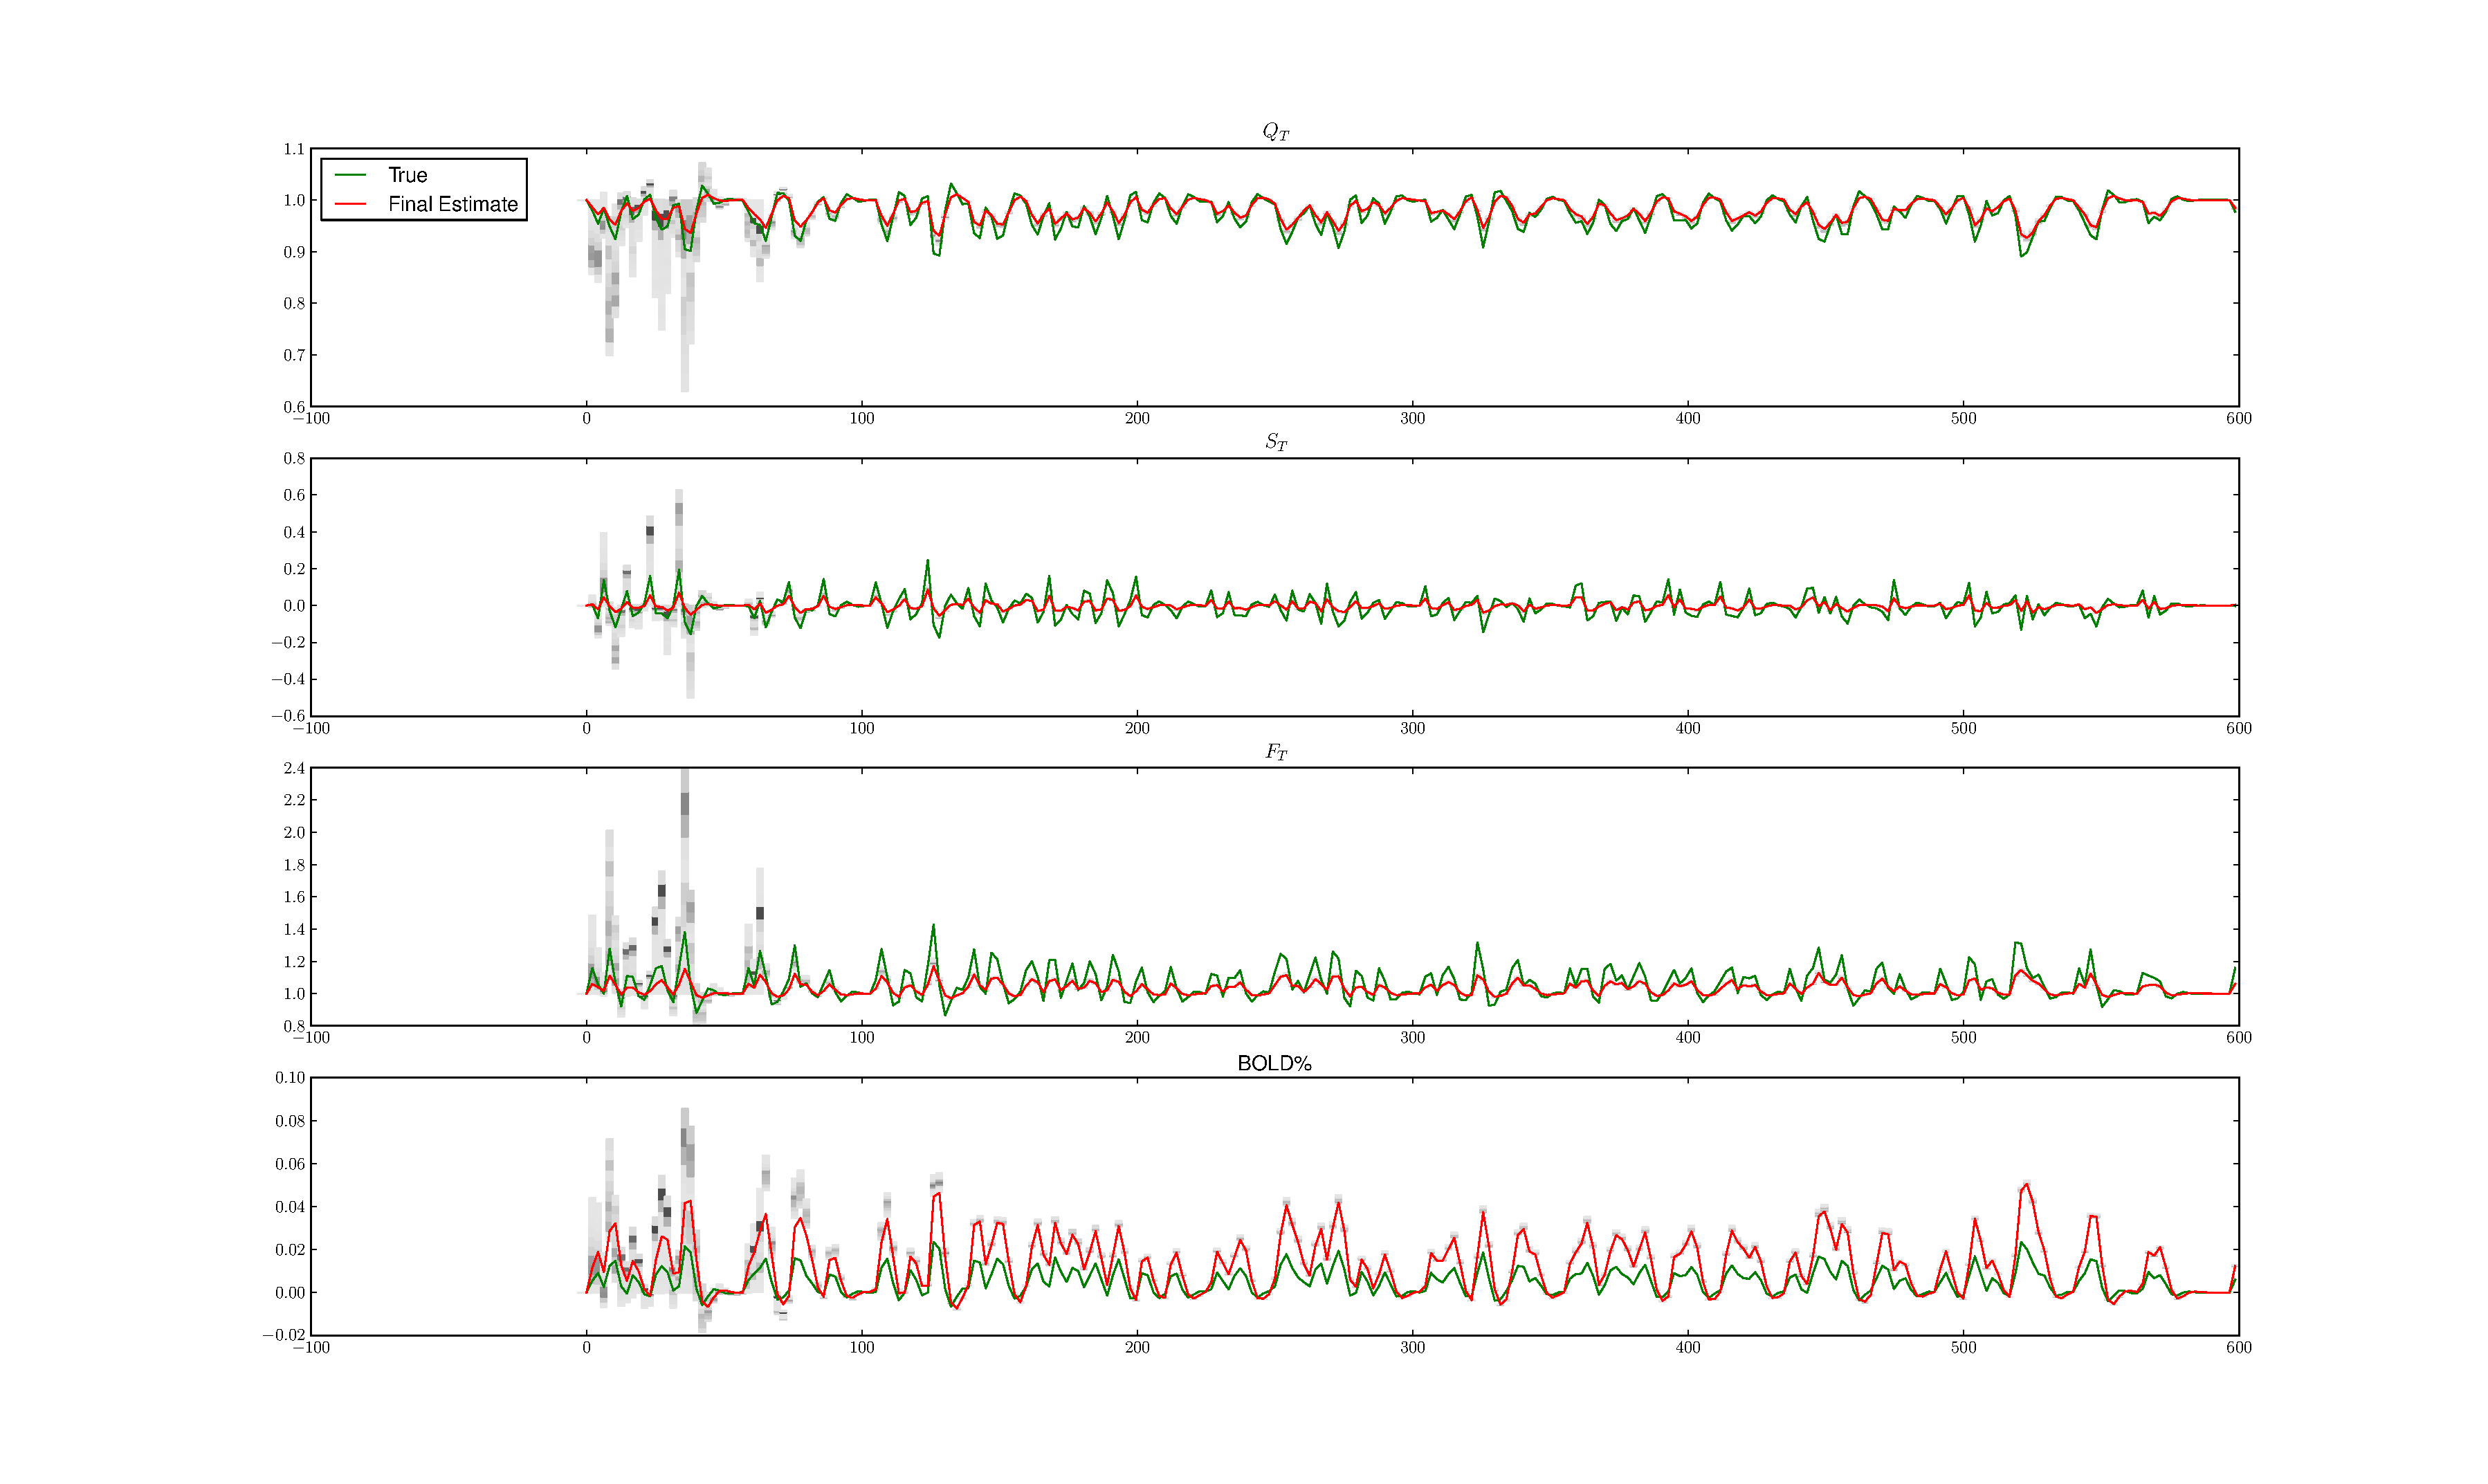
\includegraphics[trim=7cm 3cm 7cm 2cm, width=15cm]{images/highnoise_run5_3}}
\label{fig:ConvergenceRuns1}
\caption{Converging histogram for parameters during run 2, as in \autoref{fig:NoiseComparisonJustTwo}.}
\end{figure}

There are a number of interesting convergence properties of the
particle filter when more noise is present, as both \autoref{fig:ConvergenceRuns1} and
\autoref{fig:ConvergenceRuns2} show. Obviously the particle filter seems to converge
significantly faster, as points tend to be further out on the weighting function. This
also causes significantly more resampling which is the explanation for the seeming
jumps in resolution that occur from time to time. 

\begin{figure}[H]
\subfigure[$\tau_0$, $\alpha$, $E_0$, $V_0$]
{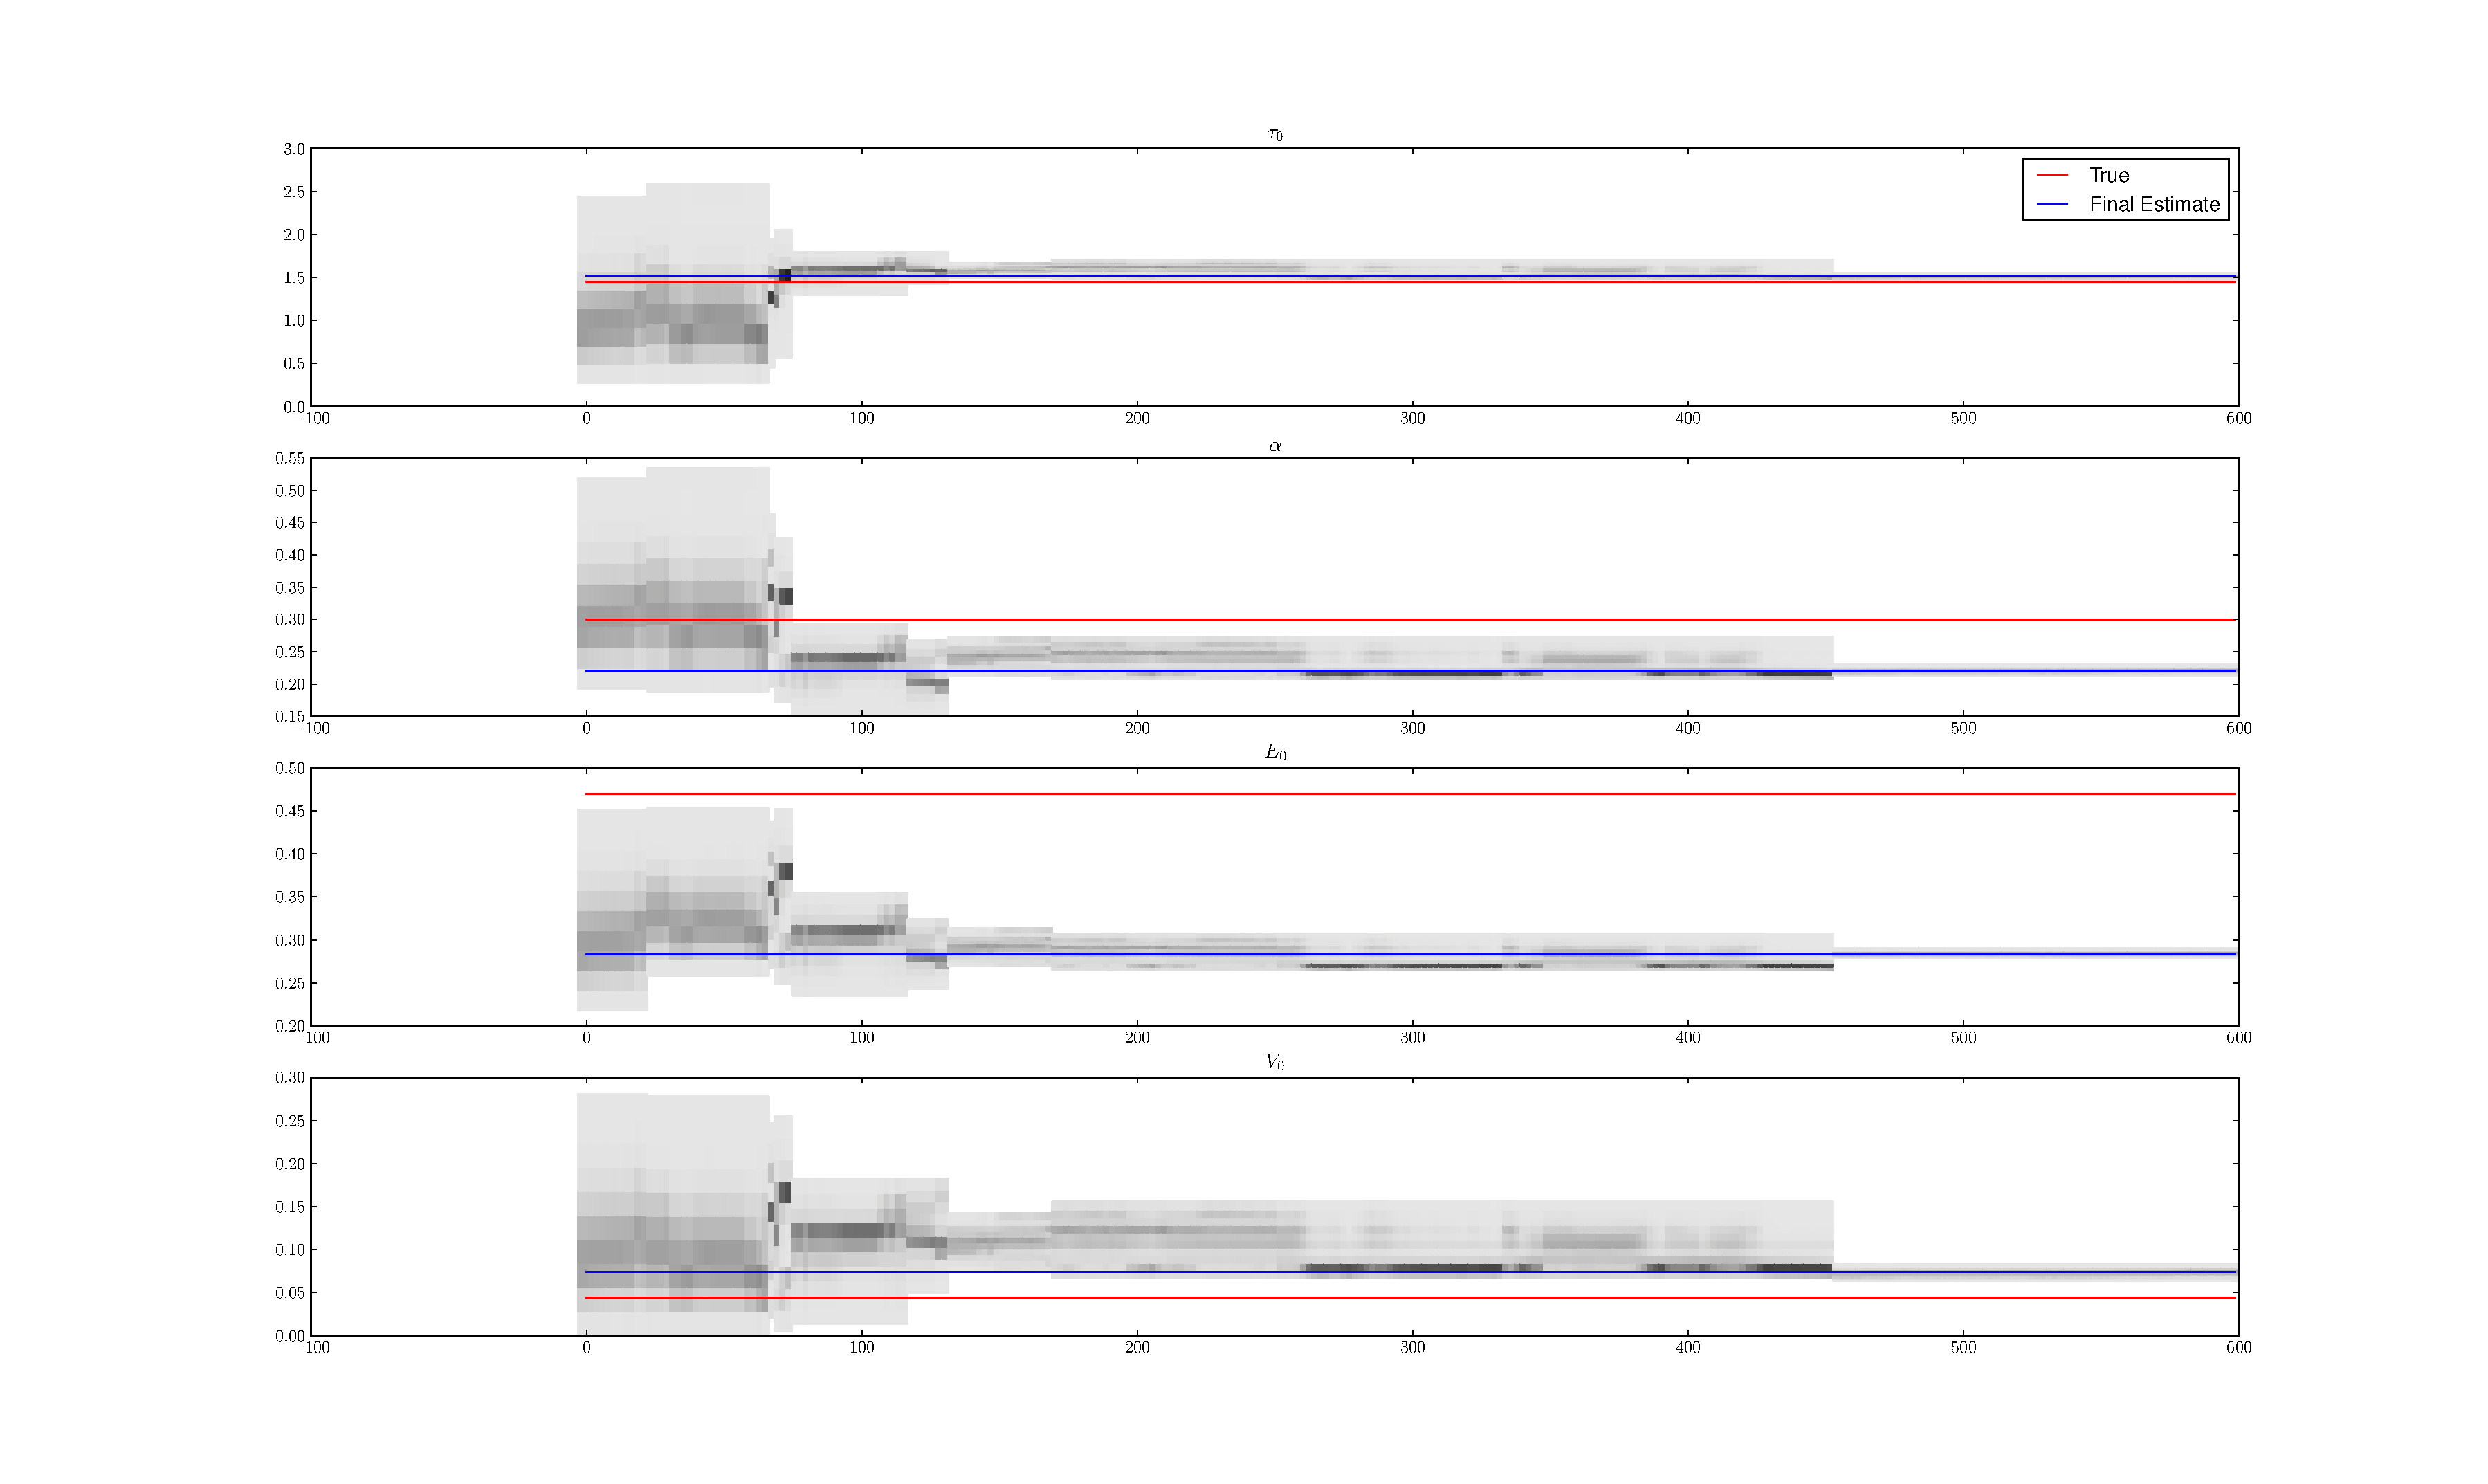
\includegraphics[trim=7cm 3cm 7cm 4cm, width=15cm]{images/highnoise_run6_1}}\\
\end{figure}
\begin{figure}[H]
\subfigure[$\tau_s$, $\tau_f$, $\epsilon$, $V$] 
{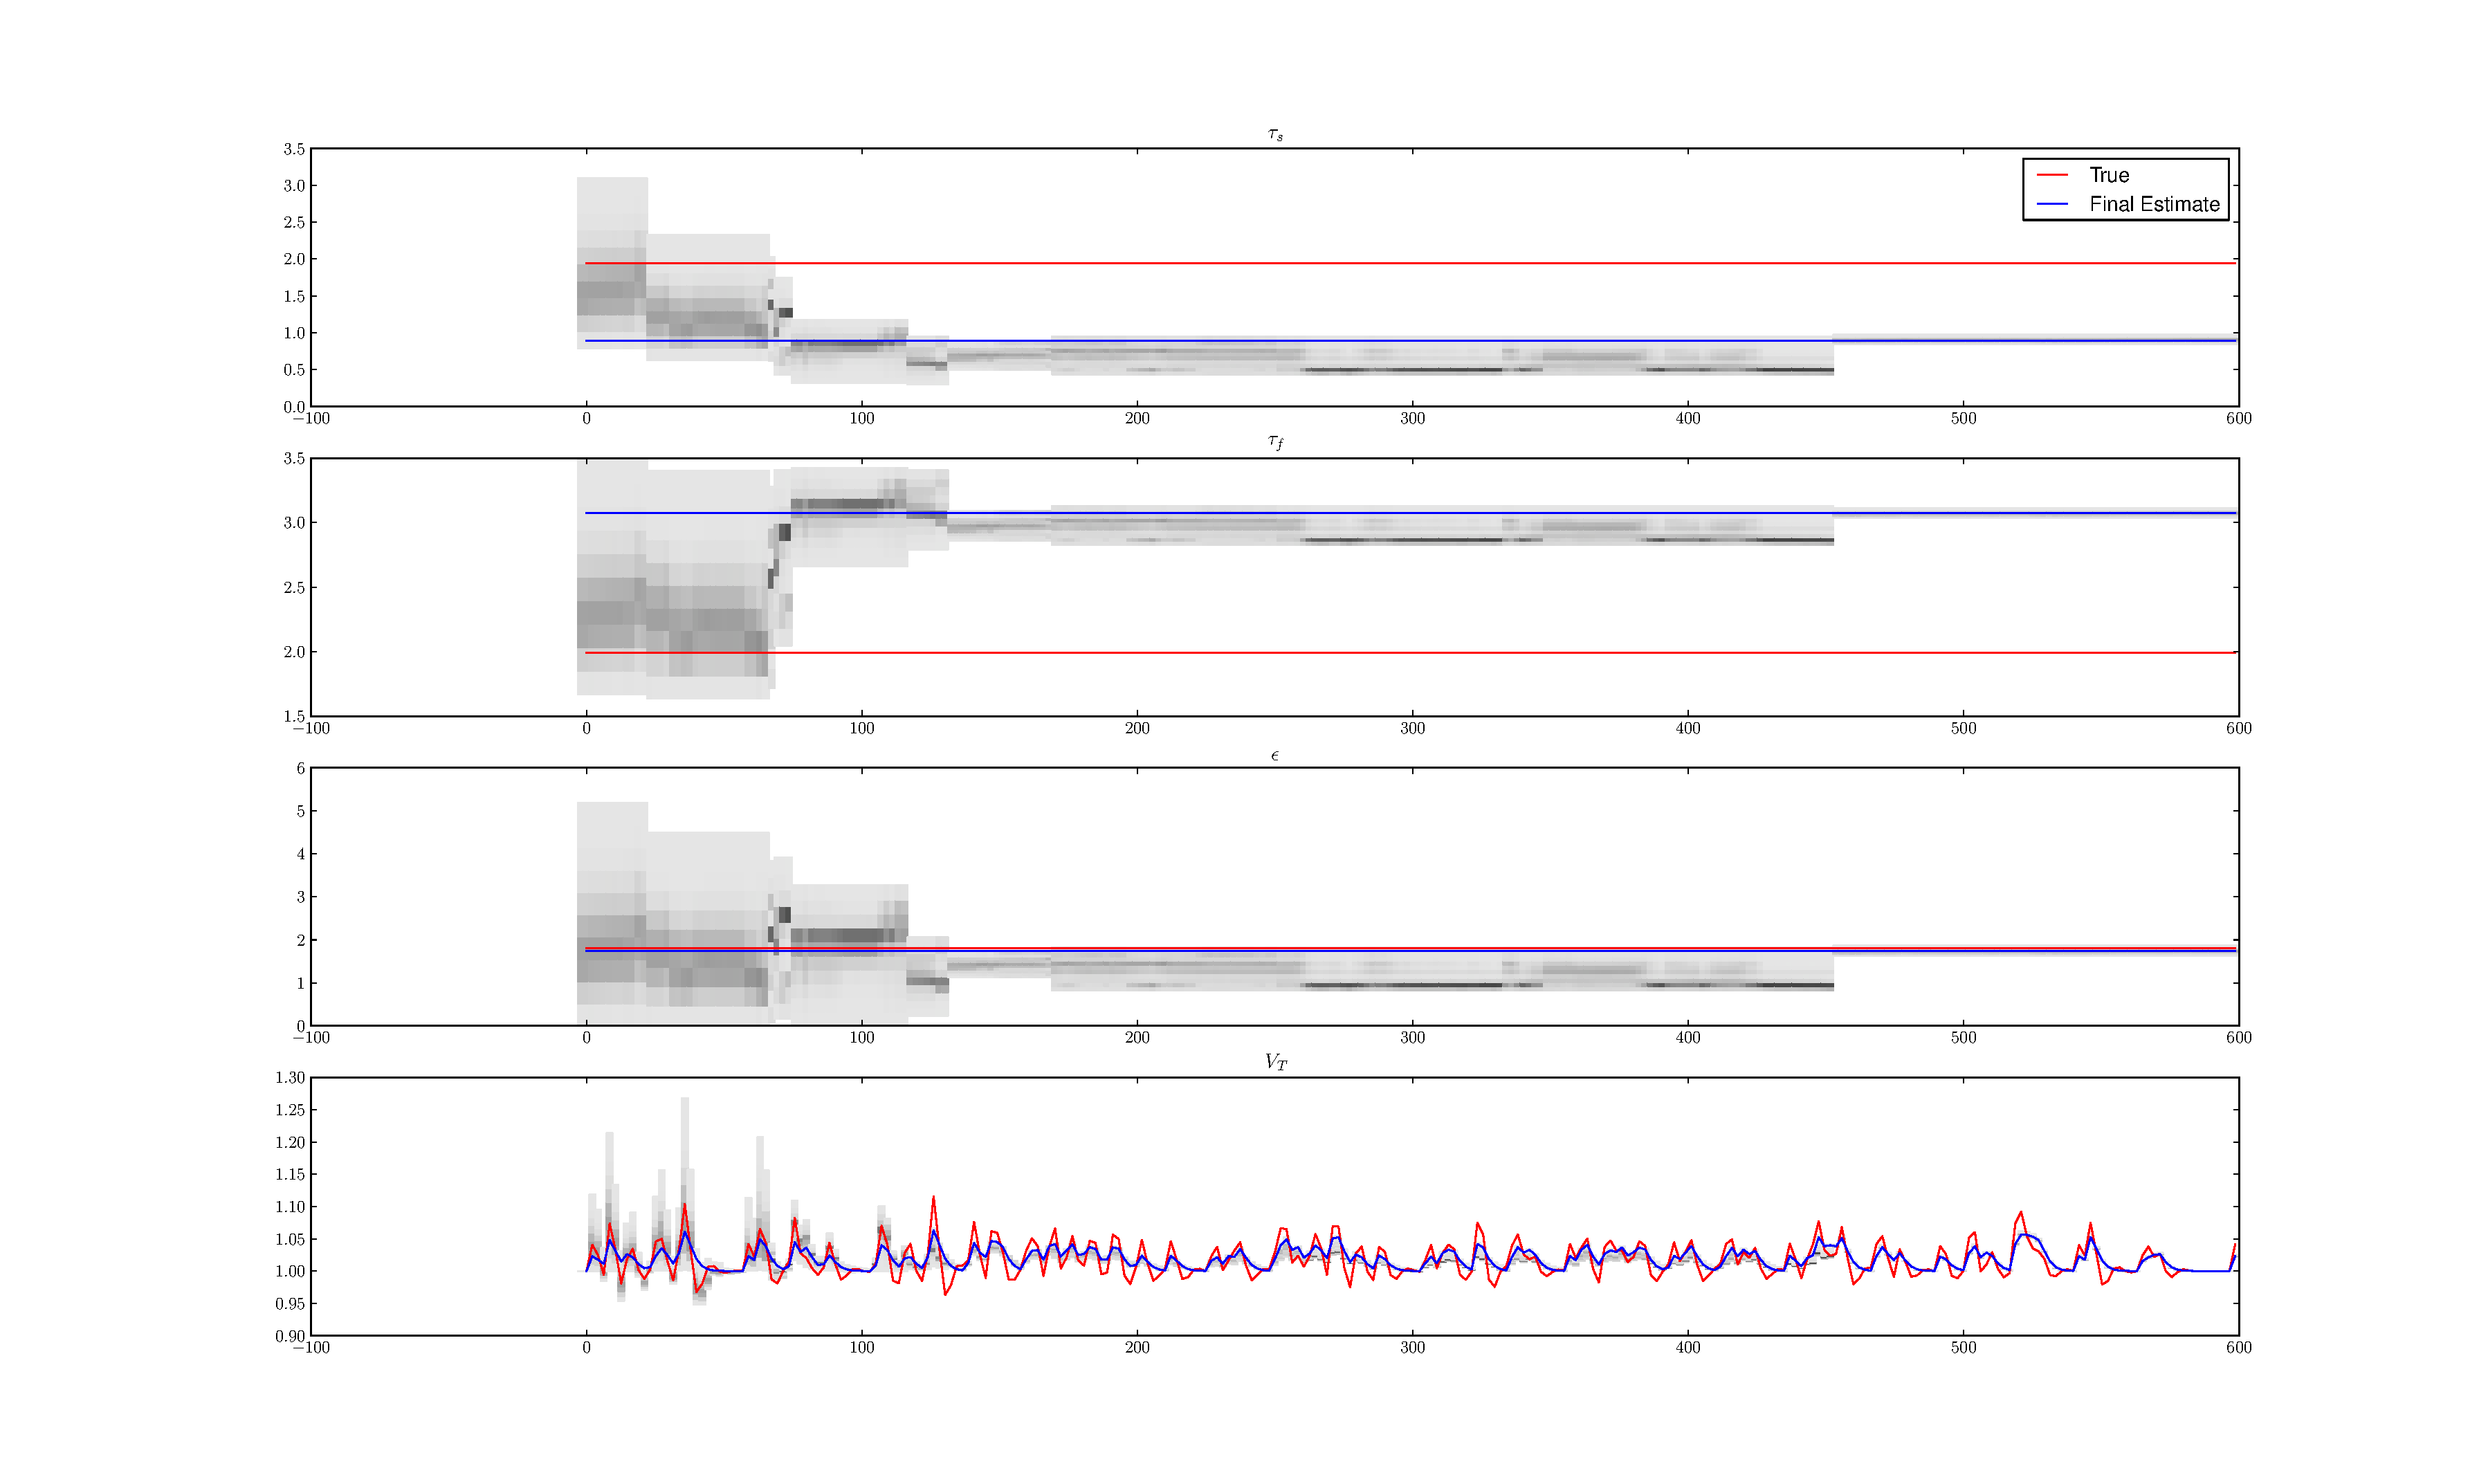
\includegraphics[trim=7cm 3cm 7cm 1cm, width=15cm]{images/highnoise_run6_2}}\\
\end{figure}
\begin{figure}[H]
\subfigure[$Q$, $S$, $F$, $BOLD$ ]
{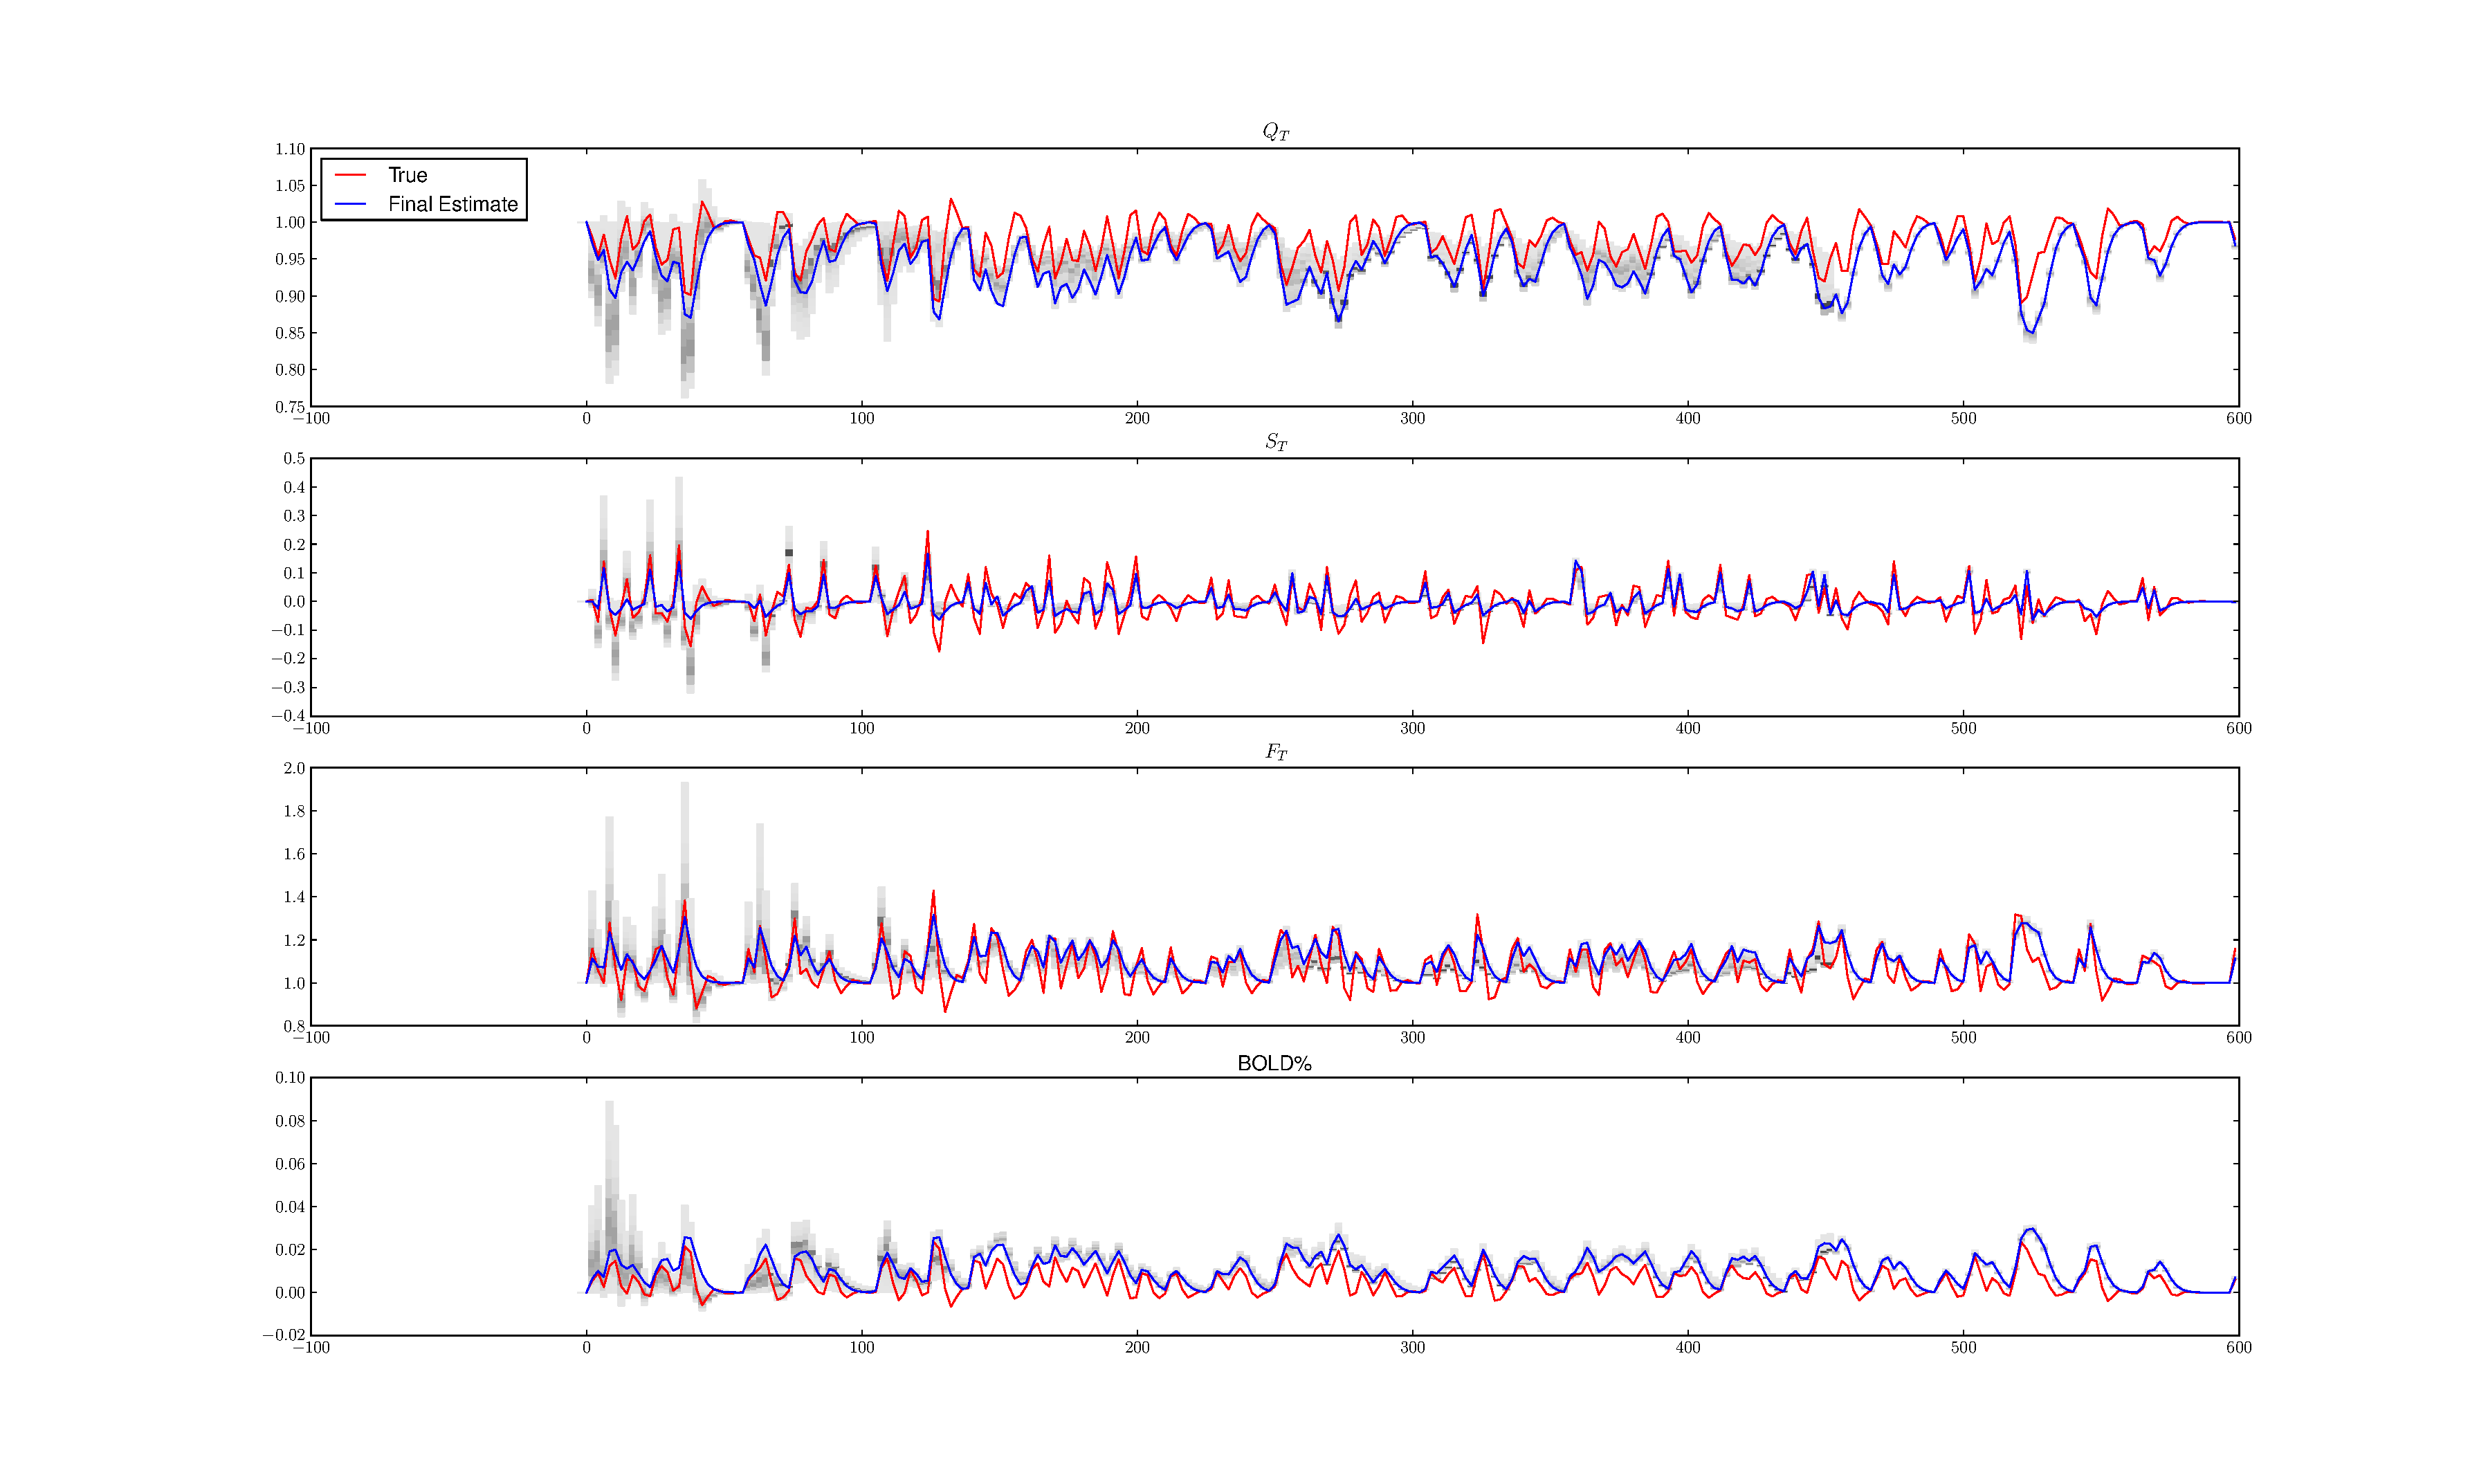
\includegraphics[trim=7cm 3cm 7cm 2cm, width=15cm]{images/highnoise_run6_3}}
\label{fig:ConvergenceRuns2}
\caption{Converging histogram for parameters during run 2, as in \autoref{fig:NoiseComparisonJustTwo}.}
\end{figure}

The parameters arrived at for all ten filter runs are shown in \autoref{tab:HighNoiseResults}.

\begin{table}[t]
\centering
\begin{tabular}{|c | c | c | c | c | c | c | c | c | c |}
\hline 
$\tau_0$ & $\alpha$ & $E_0$    & $V_0$    & $\tau_s$ & $\tau_f$ & $\epsilon$  & $ \sum \tau $ & $\sqrt{MSE}$ (Res.) & $\sqrt{MSE}$\\
\hline 
\rowcolor[gray]{.8}
1.45 & .3 & .47 & .044 & 1.94 & 1.99 & 1.8  & 5.38 &  & \\
\hline 
\hline 
1.19002 & 0.23495 & 0.42228 & 0.128 & 1.01468 & 2.47795 & 1.11677 & 4.68265   &0.0140648  &0.01572919   \\
0.9721 & 0.21902 & 0.30505 & 0.061 & 0.57801 & 1.99596 & 3.46135 & 3.54608    &0.0137314  &0.01377685   \\
1.57947 & 0.14153 & 0.33798 & 0.1079 & 0.5843 & 2.12475 & 1.78343 & 4.28852   &0.01275372 &0.01577449   \\
1.10937 & 0.2374 & 0.53491 & 0.0351 & 1.21862 & 3.07365 & 2.35039 & 5.40164   &0.0167258  &0.0115433    \\
1.10712 & 0.27535 & 0.33651 & 0.03161 & 1.50567 & 2.65181 & 4.19099 & 5.2646  &0.01369793 &0.01221607   \\
0.58026 & 0.47931 & 0.41354 & 0.11894 & 0.97563 & 3.69018 & 1.00084 & 5.24607 &0.01149511 &0.01315637   \\
\rowcolor[rgb]{.9,.5,.5}
1.29515 & 0.25957 & 0.27559 & 0.25952 & 1.70265 & 2.8458 & 0.66172 & 5.84361  &0.01555035 &0.01789781   \\
\rowcolor[rgb]{.5,.5,.9}
1.5185 & 0.21987 & 0.28348 & 0.07417 & 0.88822 & 3.07706 & 1.73929 & 5.48378  &0.01205351 &0.01246202   \\
0.68736 & 0.3283 & 0.39786 & 0.15614 & 1.07781 & 3.1158 & 0.66432 & 4.88097   &0.01510364 &0.01257713   \\
1.01703 & 0.28497 & 0.34741 & 0.05672 & 1.58774 & 2.65157 & 2.28519 & 5.25634 &0.012493   &0.01343459   \\
0.99247 & 0.29795 & 0.32207 & 0.20943 & 0.42757 & 2.21081 & 1.01674 & 3.63085 &0.01216522 &0.01505545   \\
\hline                                                                          
1.09535 & 0.27075 & 0.36152 & 0.11259 & 1.05099 & 2.71958 & 1.84282 & 4.86592 &0.01362132  &0.01396575\\
\hline 
\end{tabular}
\caption{Estimated Parameters on 10 different runs with high noise. First row is the true parameters.
Note also that the blue row is Run 1 and the red row is Run 2, as used named this section}
\label{tab:HighNoiseResults} 
\end{table}

a series of tests to determine the convergence rate of the particle filter, the number
of particles that were required, how weighting functions compared, how different de-trending
methods compared with each other and, finally the variance of the result. By running the exact
time-series with different noise realizations, it was possible to determine the model variance.
As the reader may know, the error of an estimator may be calculated as:
\begin{equation}
MSE(\Theta) = Var(\Theta) + Bias(\Theta)^2
\end{equation}
The variance is an expression of how much the result would change for different noise realizations,
whereas the bias is an expression of how well the model matches the true underlying model. In
this case, because the same model is being used in the particle filter and underlying simulation,
the bias is actually zero. Obviously when this is calculated using \emph{real} data with an unknown
underlying state space equation, there will be some amount of bias error, but assuming that the
noise is similar to the noise used in these tests, the model variance will actually be about the
same. Thus calculating the model variance is extremely helpful in calculating how well determined
our model is, and how consistent it will be for real data. A single timeseries, as opposed to the
thousands present in a real image, makes it easier to 
compare the output with the ground truth, with various parameters. 

Second I used a modified version of the FSL tool 
POSSUM to generate an entire FMRI image from a parameter map. The parameter map was generated
by taking an existing activation map and assigning discrete parameter sets to each region.
The result was a four dimensional (length x width
x height x parameter) image with spatially varying parameters. Possum was then modified
to take a parameter map and generate activation levels depending on the parameters at that
point. The patch for POSSUM will be made available. As an unfortunate side effect of 
not using Possums' original activation scale, I manually added 750 to the total level of
simulated Possum images. This is because the BOLD \% difference levels were in the range
of 50 - 100\% from the base, about 5 times as large as they should have been. Ultimately
this should not have an effect on the parameters (other than perhaps $\epsilon$ and $V_0$). 
For each time-series in the simulated FMRI image, the final \emph{static} parameters were saved
into a parameter map. This parameter map may then be compared to the map used to generate the 
simulated data; additionally a new simulation using the calculated parameters may also be 
generated to test the difference in activation levels between the real parameters and the
estimated ones. Since it is clear that the parameters are not fully orthogonal 
(\cite{Deneux2006}), its possible that two sets of parameters are functionally equivalent,
but have different parameters. This way, an absolute 
quantitative difference between the two parameter sets may be found.

\section{Real Data}
Finally, we also performed inference based on real FMRI data. The scanner we used...
%... more specifics...

Before performing tests on a full image, I tested the results of the particle filter
on regions deemed active and non-active by statistical parametric mapping. 
\section{Single-Voxel Simulation}
The results 

\section{Single-Voxel Analysis}
This section discusses the results when the particle filter was
applied on a single voxel. The parameters are the same as
those used later for entire image analysis; however, the results
are more in-depth. 

The run-time for a single voxel depends on the several factors. First, the
overall length of the signal being analyzed. For 1000 measurements it takes
about 10 to 15 minutes. On the other hand, in real circumstances the
length is only around 150 measurements. The number of  integration
can certainly make a large difference, however dropping below 1000 (.001 seconds)
is definitely not recommended. 

For a period I considered 1000 to be a
fine number; however when generating simulated data I found that every once
in a while 1000 was not enough. This is problematic in the actual particle
filter since, given the large number of simultaneous integrations taking 
place, its likely that a few particles will fail and be weighted at 0 because
of this problem. Additionally, because the typical case where a failure would
occur is at fast moving times/parameters the particles all tend to fail together.
The result is particle deprivation - no particles with non-zero weights remain.
The other possible outcome is that low time constant particles get pruned resulting
in excessively smoothed estimates for the time series'. Its possible that a
kind of stop-gap measure could be put into place; wherein particles that are
about to be set to NaN are integrated again with finer grained steps. However
many times the non-real results don't occur until several time steps after the 
numbers get strange. So for instance, the timestep was too long, allowing 
$f$ to go negative, resulting in extremely large values of $q$. There are many
different ways where this sort of event can occur, and unfortunately sometimes
there is no way to get back to before the state starting going out of control.

Another crucial factor for run time is how long before the first re-sampling 
occurs. Because the prior is represented initially with significantly more
particles, if the model fits very well, or for some reason the effective
number of particles stays high, resampling could take a long time to occur.
When this happens the particles filter can take a factor of 10 longer to run.
However, if the particle count isn't initially set high, there is a much larger
chance of particle deprivation occurring. Since there is no real way to know
how long it will take to resmaple the first time, there is little the 
algorithm can do to fix this (except perhaps forcing resampling after
some period of time). On the other end of the spectrum, if the time
series doesn't match the model at all, particle deprivation will occur extremely
quickly.  The upshot of this is that the particle filter is able to 
identify these sections very quickly, and thus not waste much time there.
The difficulty though, is the regions in between the perfect fit and the
awful fit. If particle deprivation does occur, did it occur randomly to an
activated region or did it occur inevitably because the region doesn't fit.
The reason for having so many initial particles is to give density to the
distribution to make false negatives more rare. Perhaps the correct method
is to still set the initial particles very high, but if for a long time no
resampling occurs, halve the standard deviation of the measurement error.
Thus, if the weighting function is not discriminating enough, force it 
to be more picky about the results. Of course this could lead to particle
deprivation as well if the standard deviation is brought down too quickly.
Of course, if a fat-tailed distribution is used for the weighting function,
or the standard deviation of a Gaussian weighting function is sufficiently large,
the particle filter will simply converge to meaningless values. The question
of whether 

\begin{figure}
\label{fig:badfit}
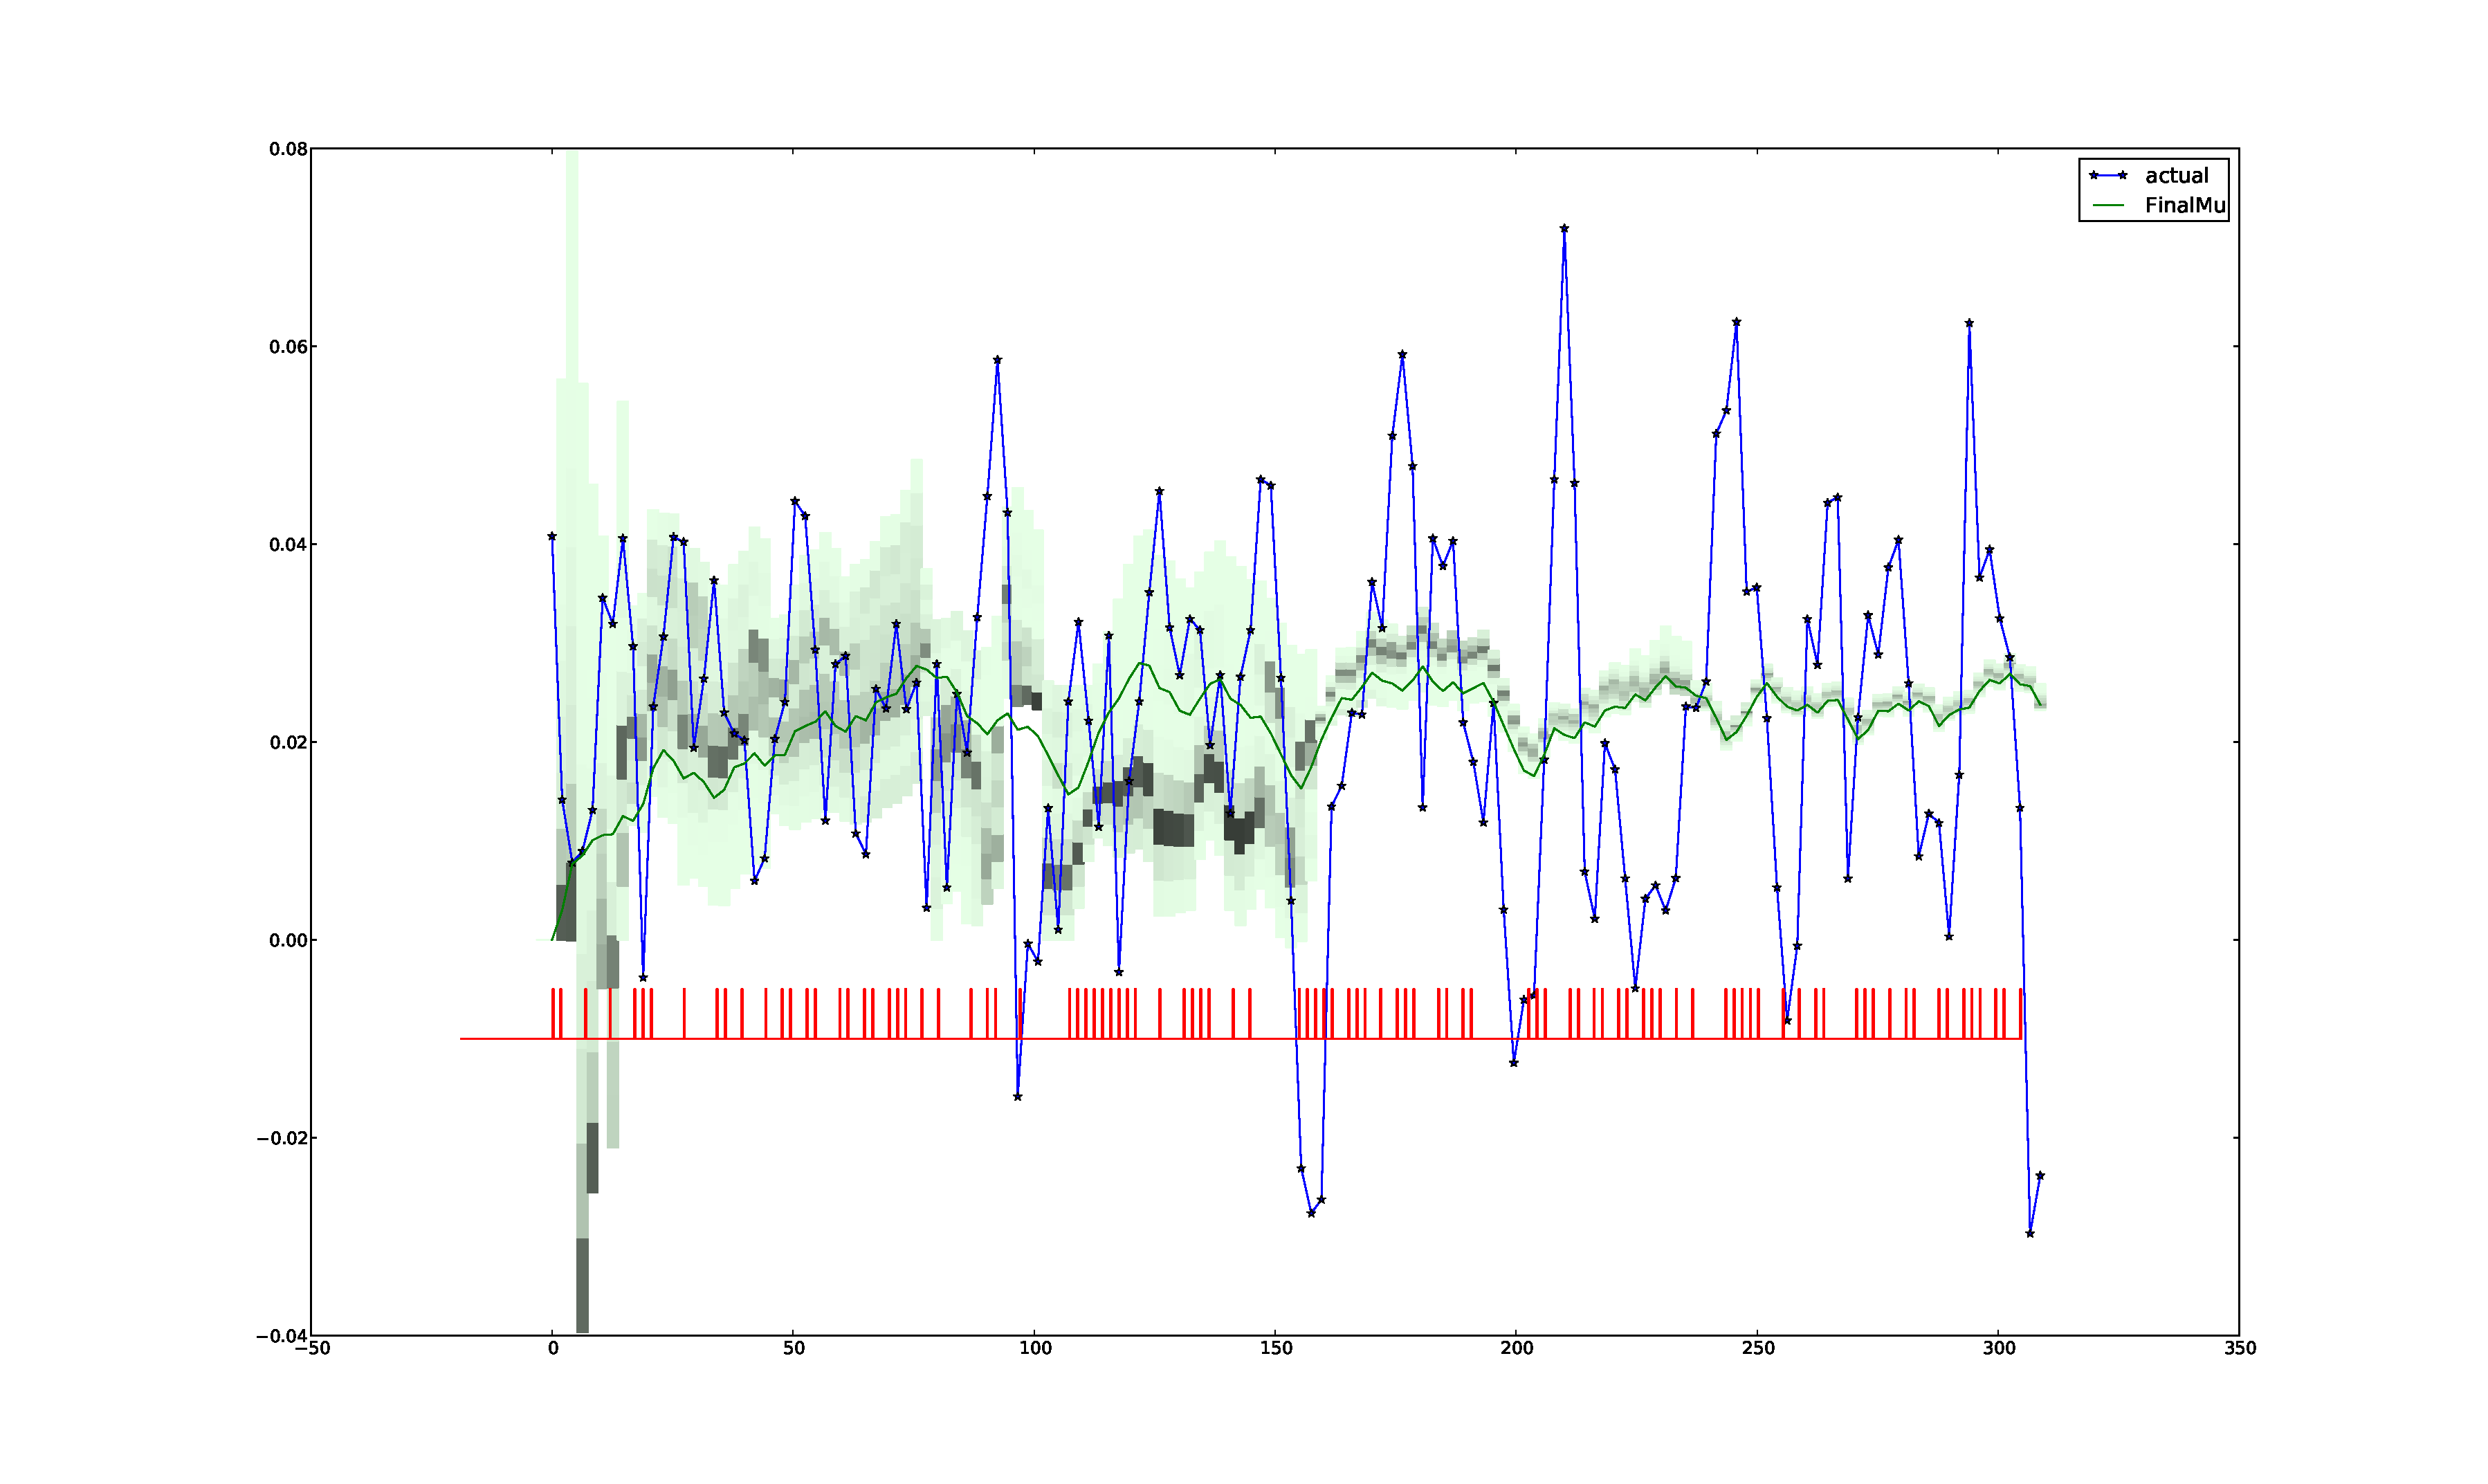
\includegraphics[trim=10cm 4cm 10cm 4cm, width=16cm]{images/inactive_illogical}
\caption{Particle Filter converging to values that make little sense,
because the voxel did not correlate with the input in any known way}
\end{figure}

\begin{figure}
\label{fig:highhard}
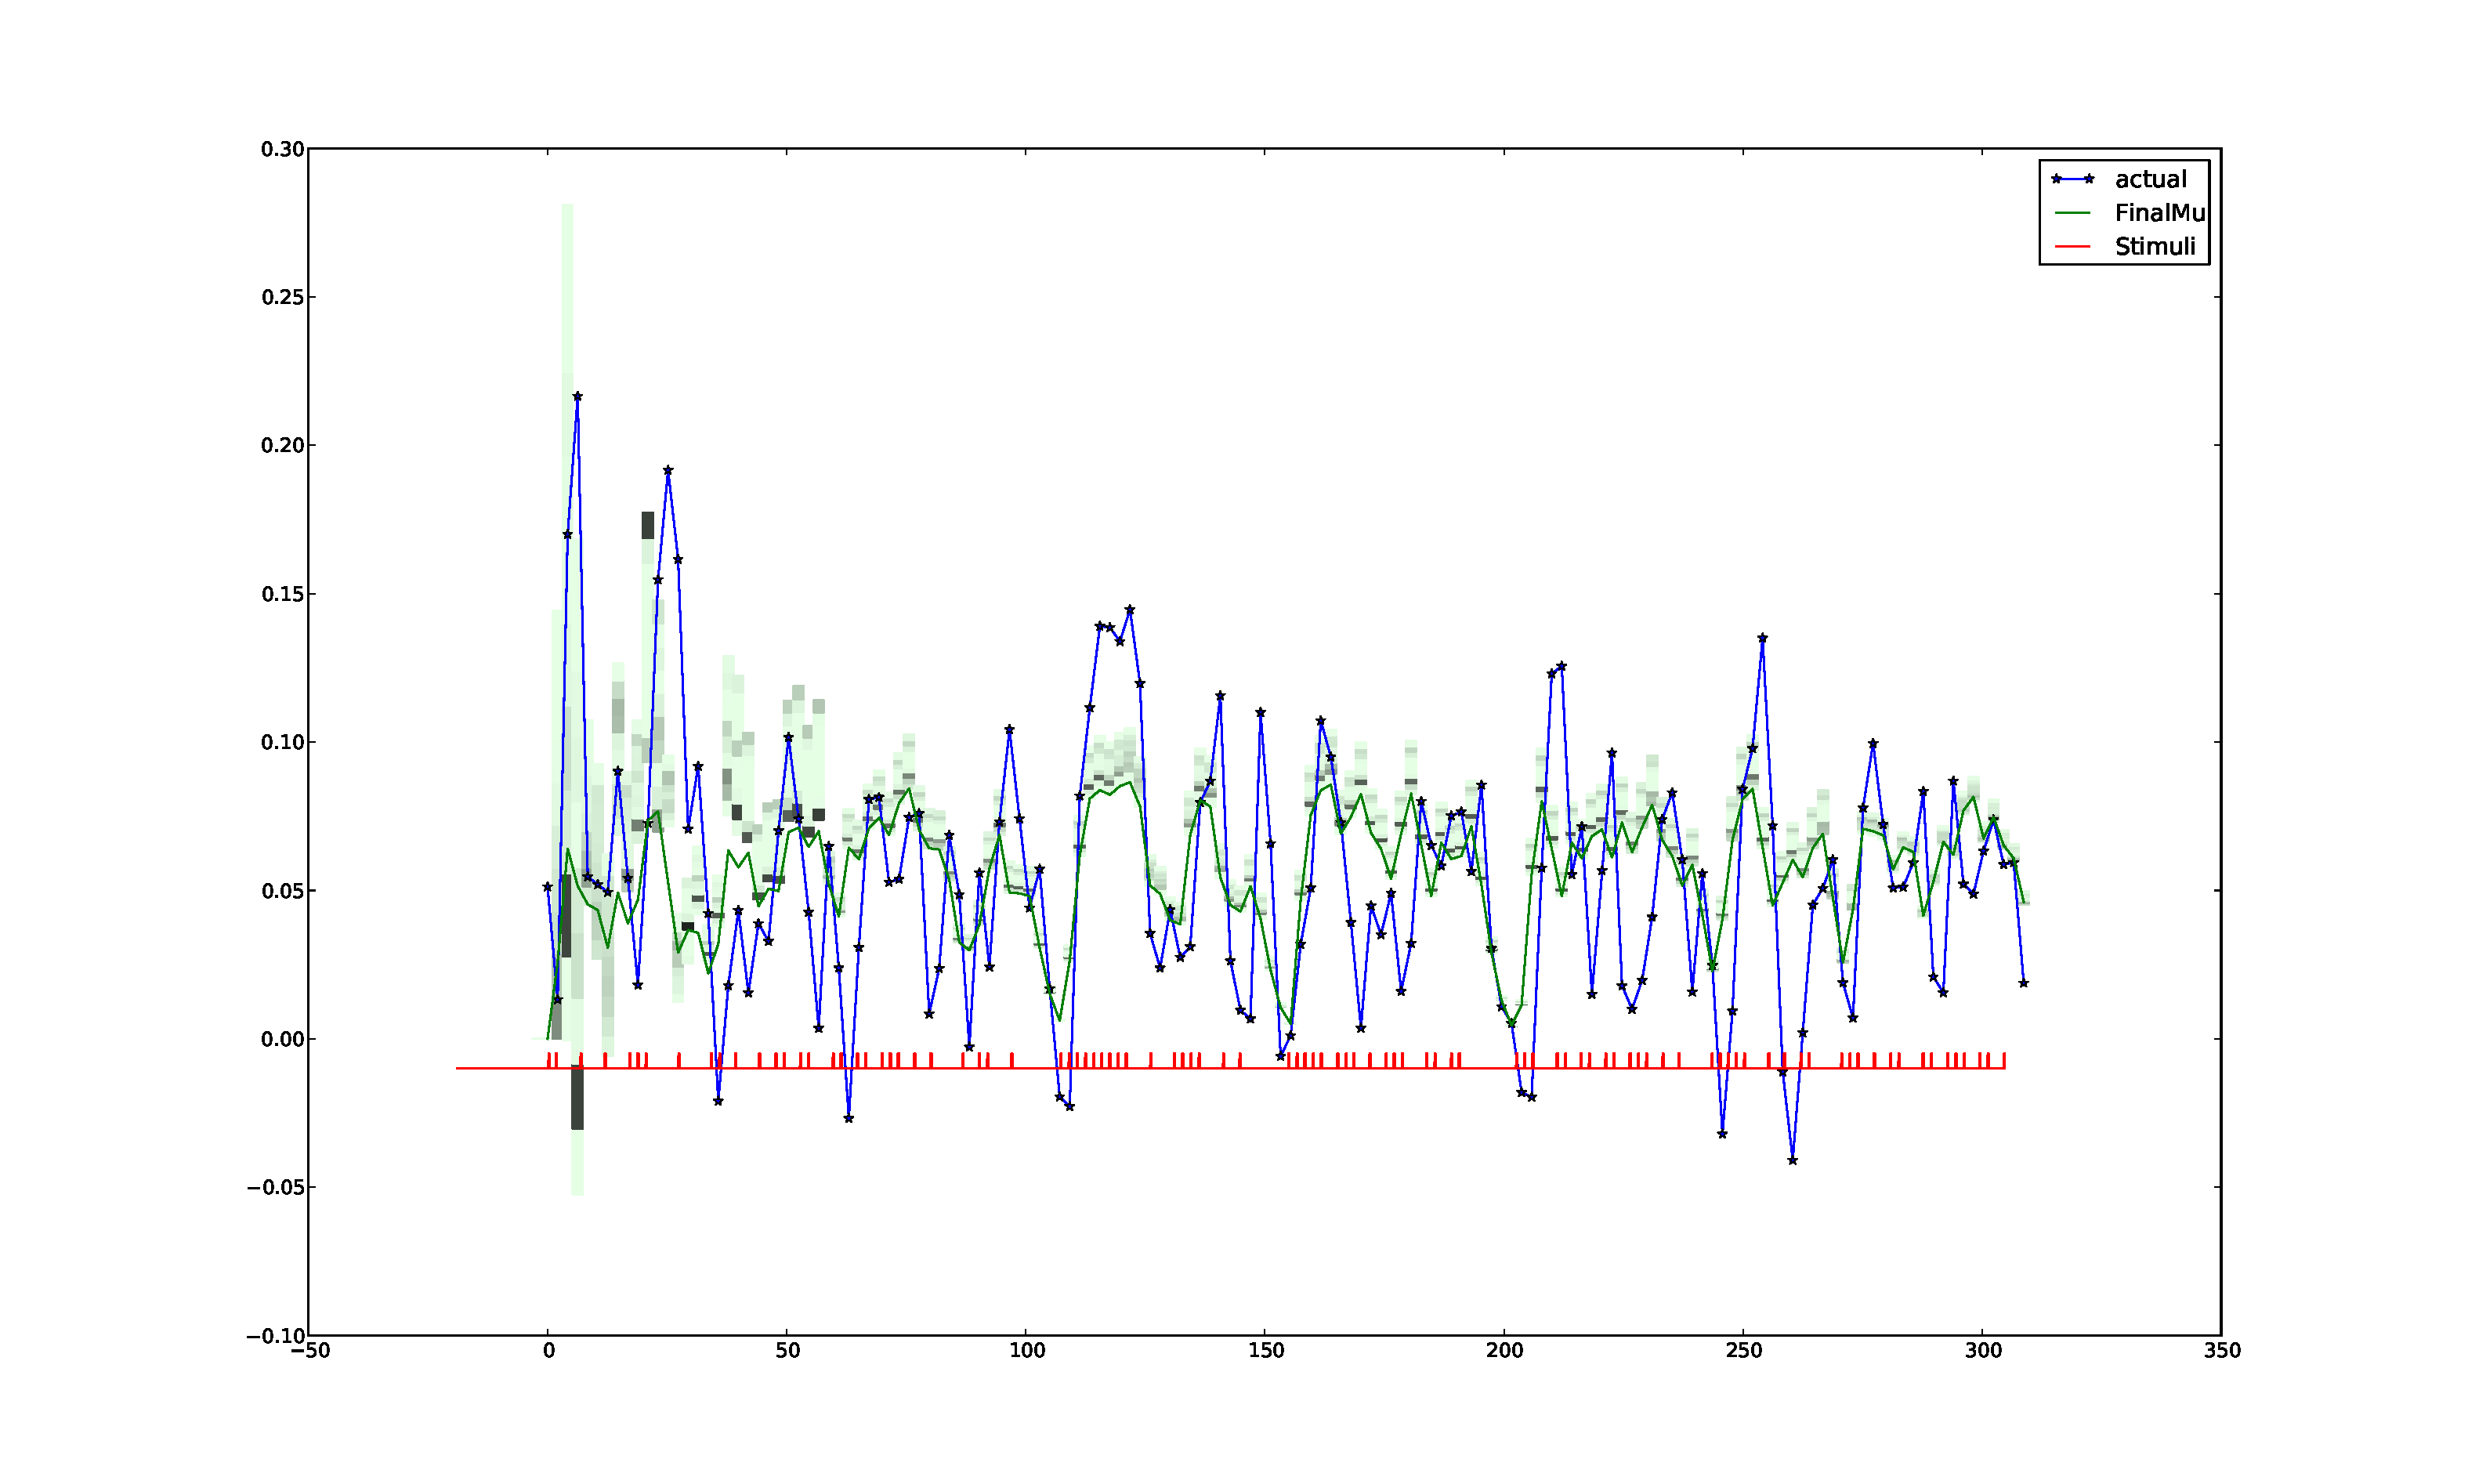
\includegraphics[trim=10cm 4cm 10cm 4cm, width=16cm]{images/active_difficult}
\caption{Example of a timeseries that laplace performs better on than
gaussian. The large spike at the beginning can quickly eliminate all particles} 

\end{figure}

For this reason, it is important to threshold based on the MSE, and the
impulse response. Naturally the MSE is intended to catch very voxels with a
very poor fit,
but like \autoref{fig:badfit}, the algorithm may have found a line
down the middle that gives a decent mean squared error. In this case
the excessive smoothing and low actual activation level will easily
be distinguished by finding the peak response to single short pulse. 

The choice of a prior, as discussed previously, is extremely important. While a
prior may have the potential to give good results, being a monte-carlo algorithm
there is the possibility for inconsistencies. Thus, increasing the variance
of the time-constants may allow additional flexibility, it will also cause
additional model variance. Case in point, the exact same algorithm run twice
with standard deviations of $.35, .35, .35$ for the time constants resulted in two
very different fits, see \autoref{fig:param1_var}.

\begin{figure}
\label{fig:badfit_param1}
\subfigure[]{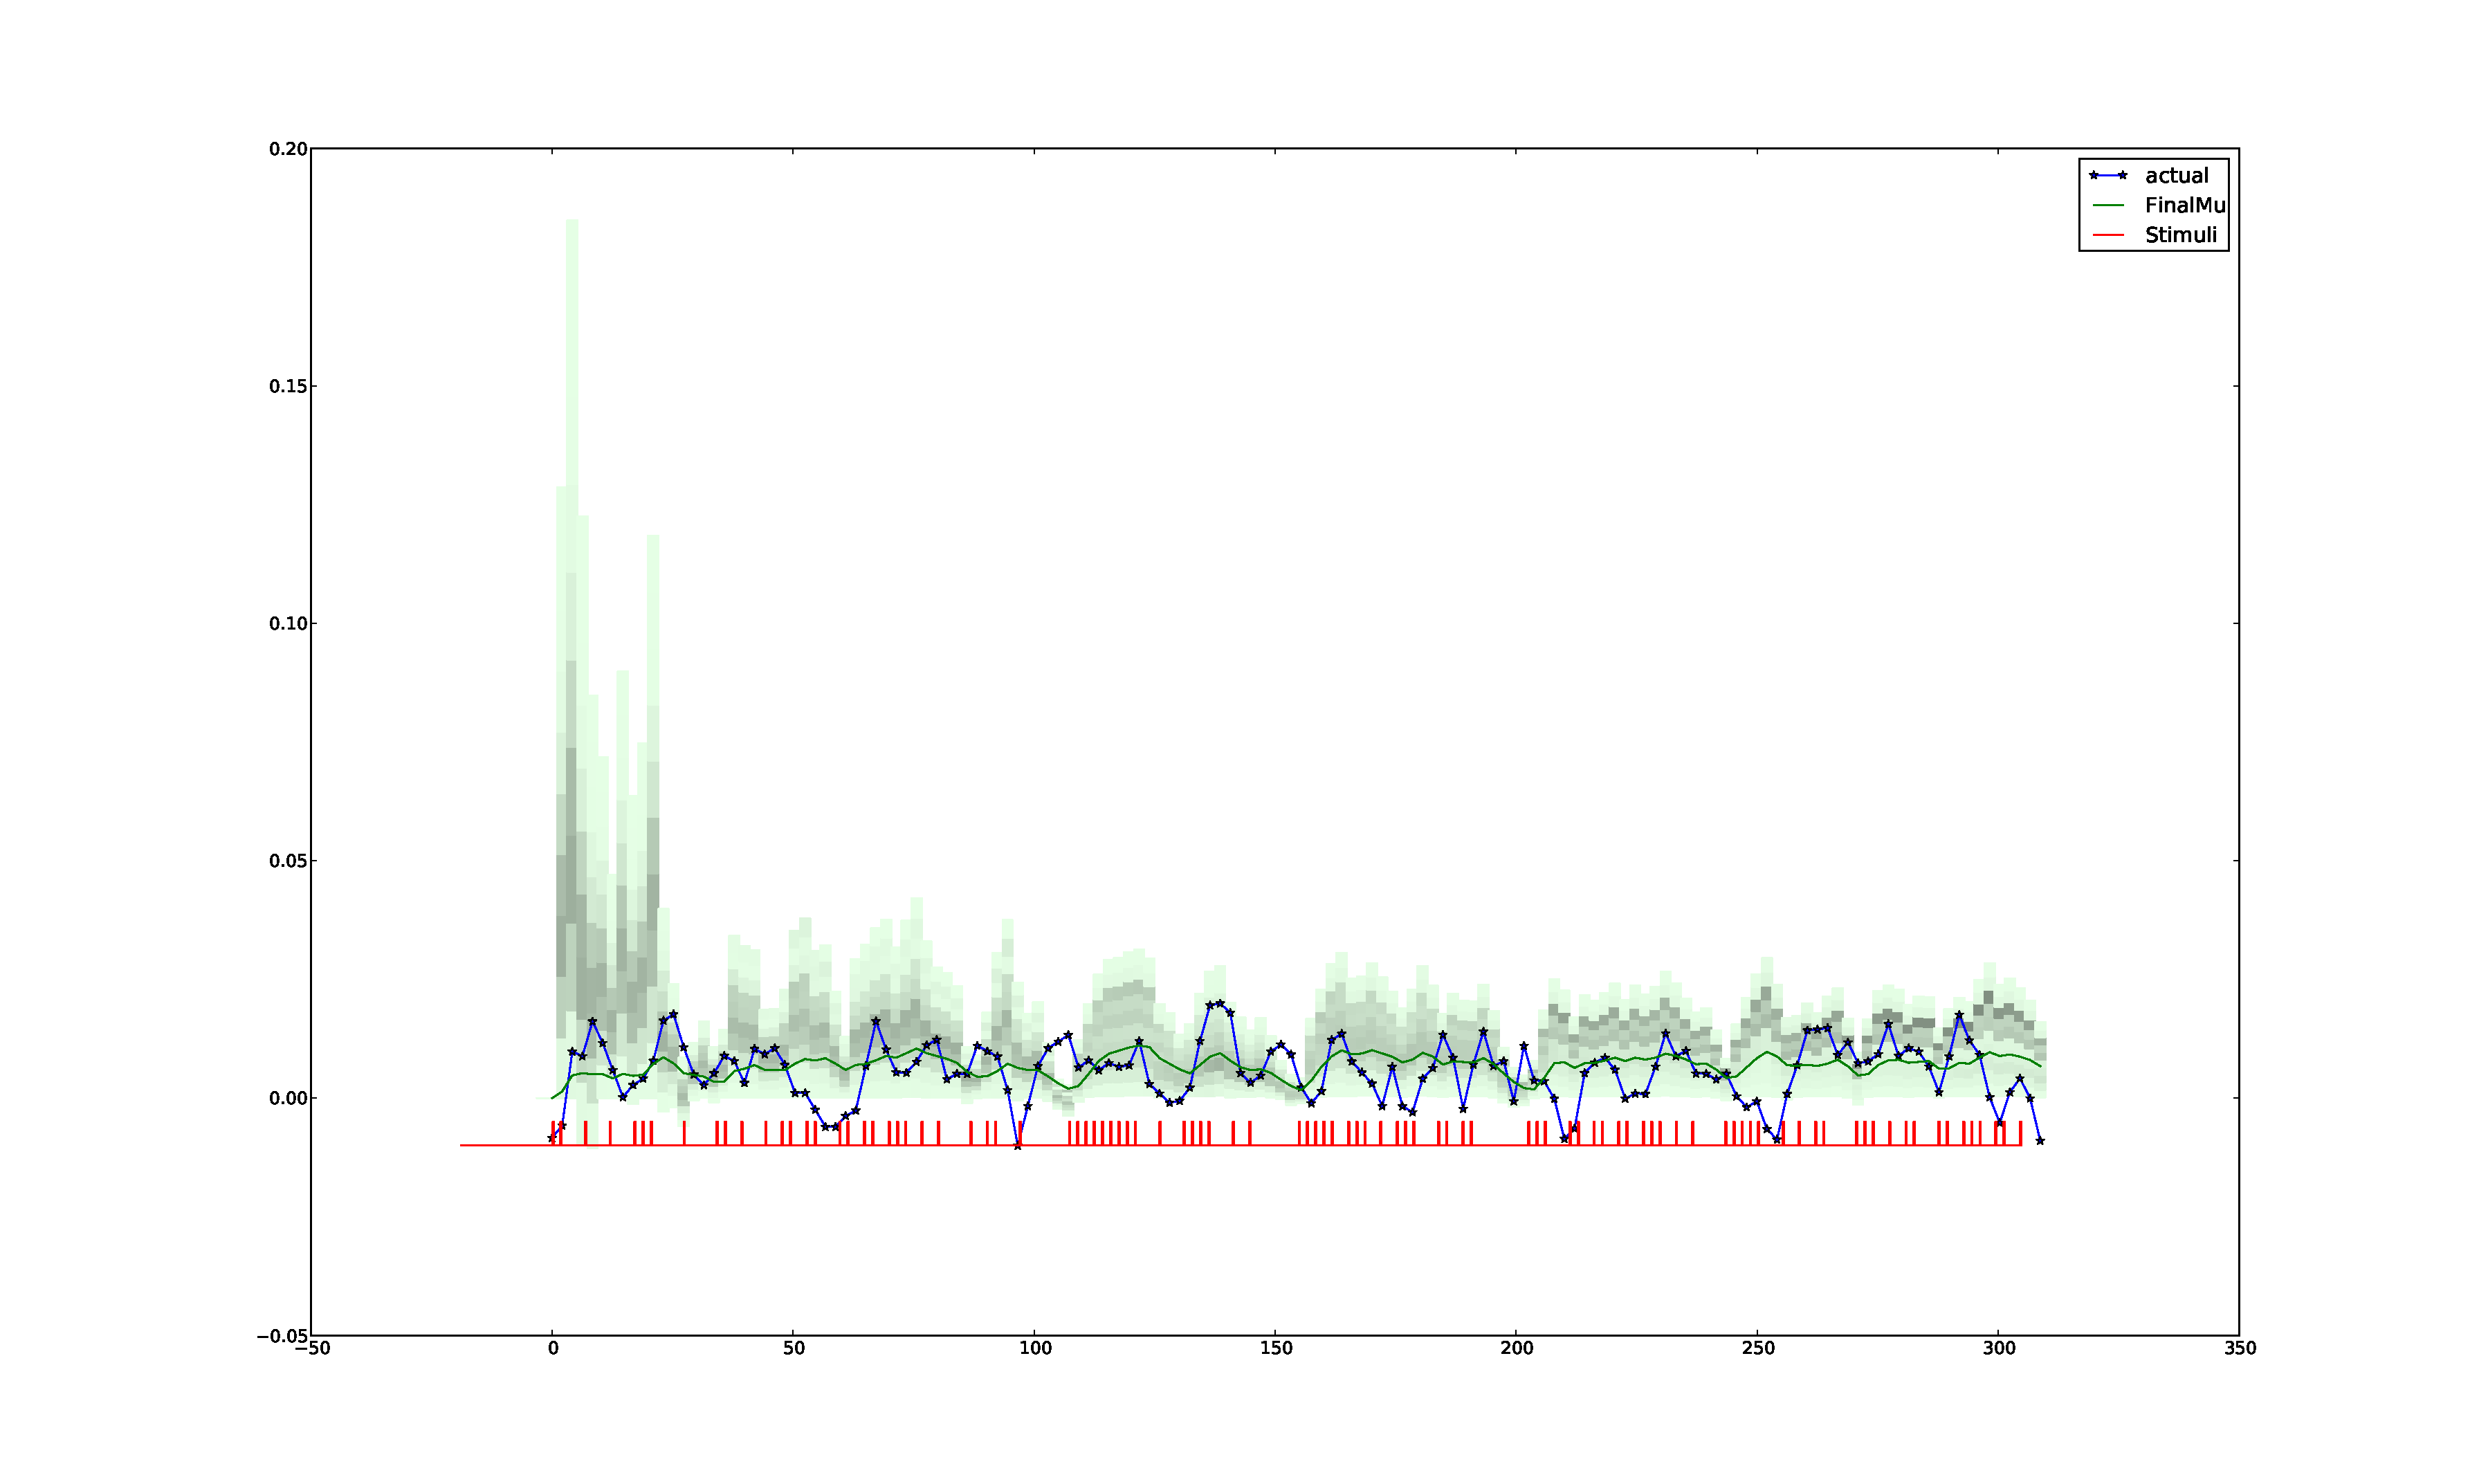
\includegraphics{images/badfit_param1}}
\subfigure[]{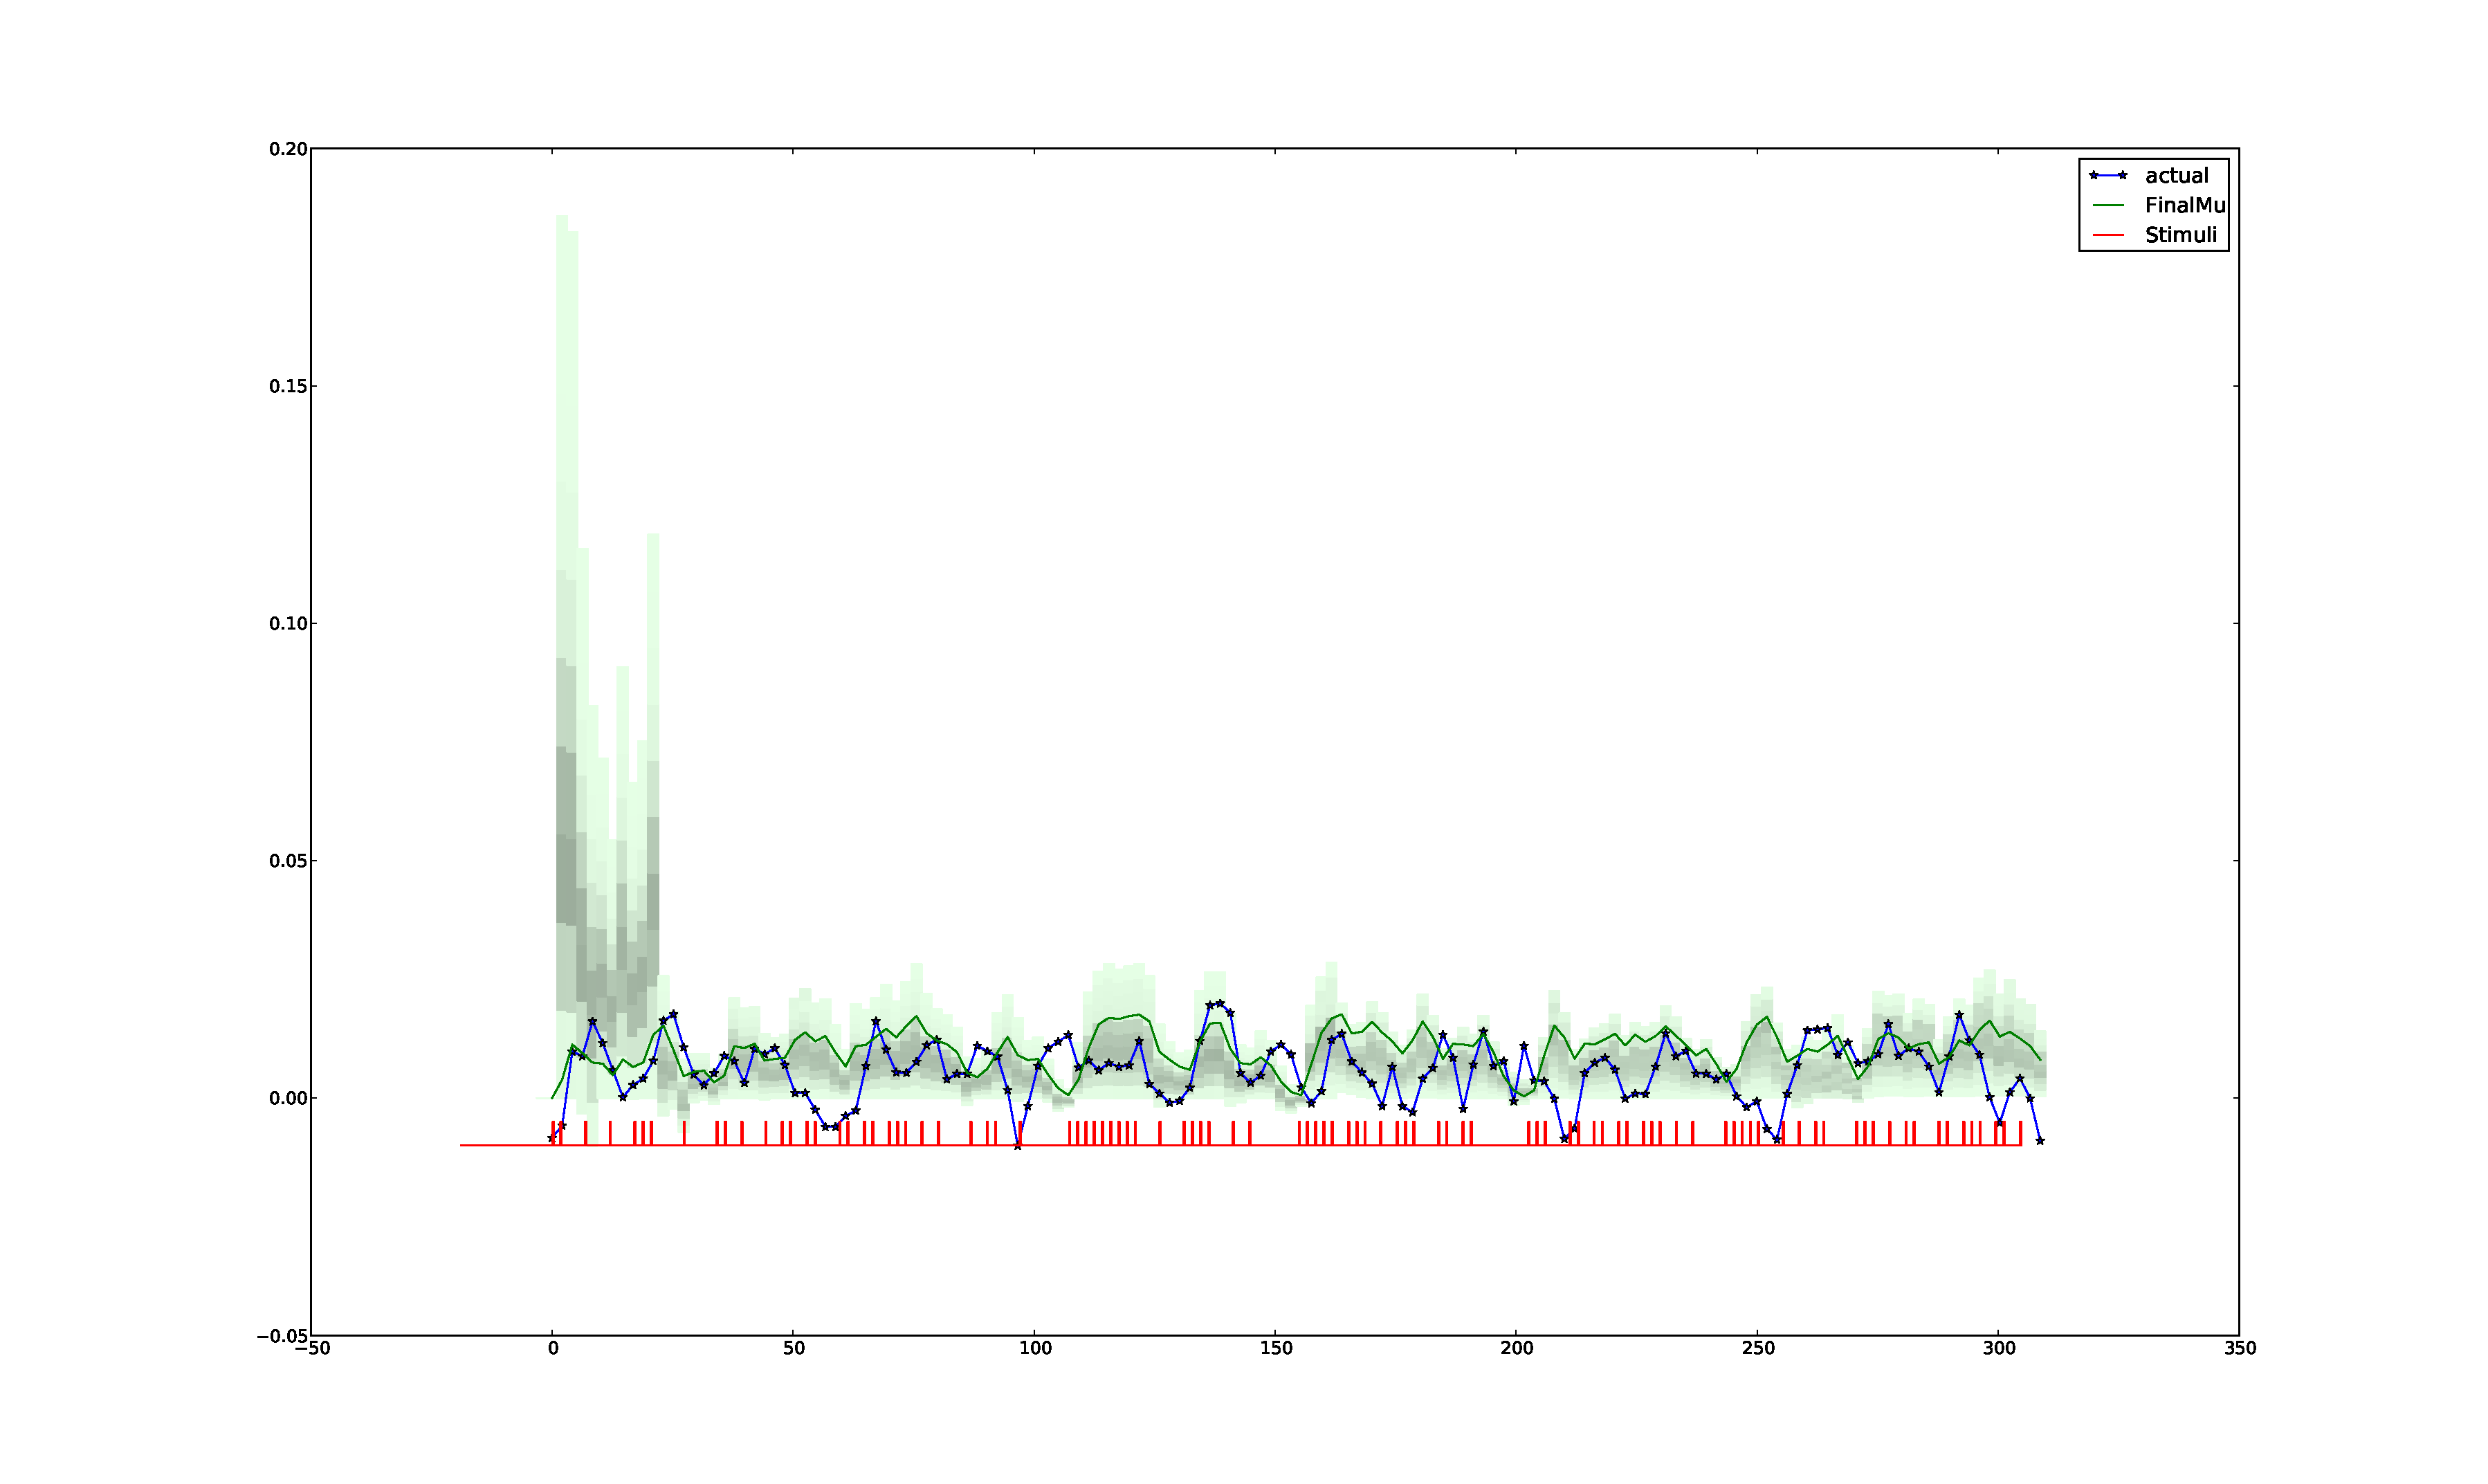
\includegraphics{images/goodfit_param1}}
\caption{The same priors gave rise to both fits. Params: ($\tau_0 \alpha E_0 V_0 \tau_f \tau_s \epsilon$)
for the good fit: $(1.40 .32 0.34 0.04  0.96 2.76)$, and for the poor fit:
$(2.28 0.32 0.33 0.017 0.67 2.88 1.36)$.}
\end{figure}

For this reason, I actually lowered the standard deviattions of the time
constants to prevent over-smoothing. This resulted in the more consistent, but
slightly worse results seen in \autoref{fig:param2_var}

\begin{figure}
\label{fig:param2_var}
\subfigure[]{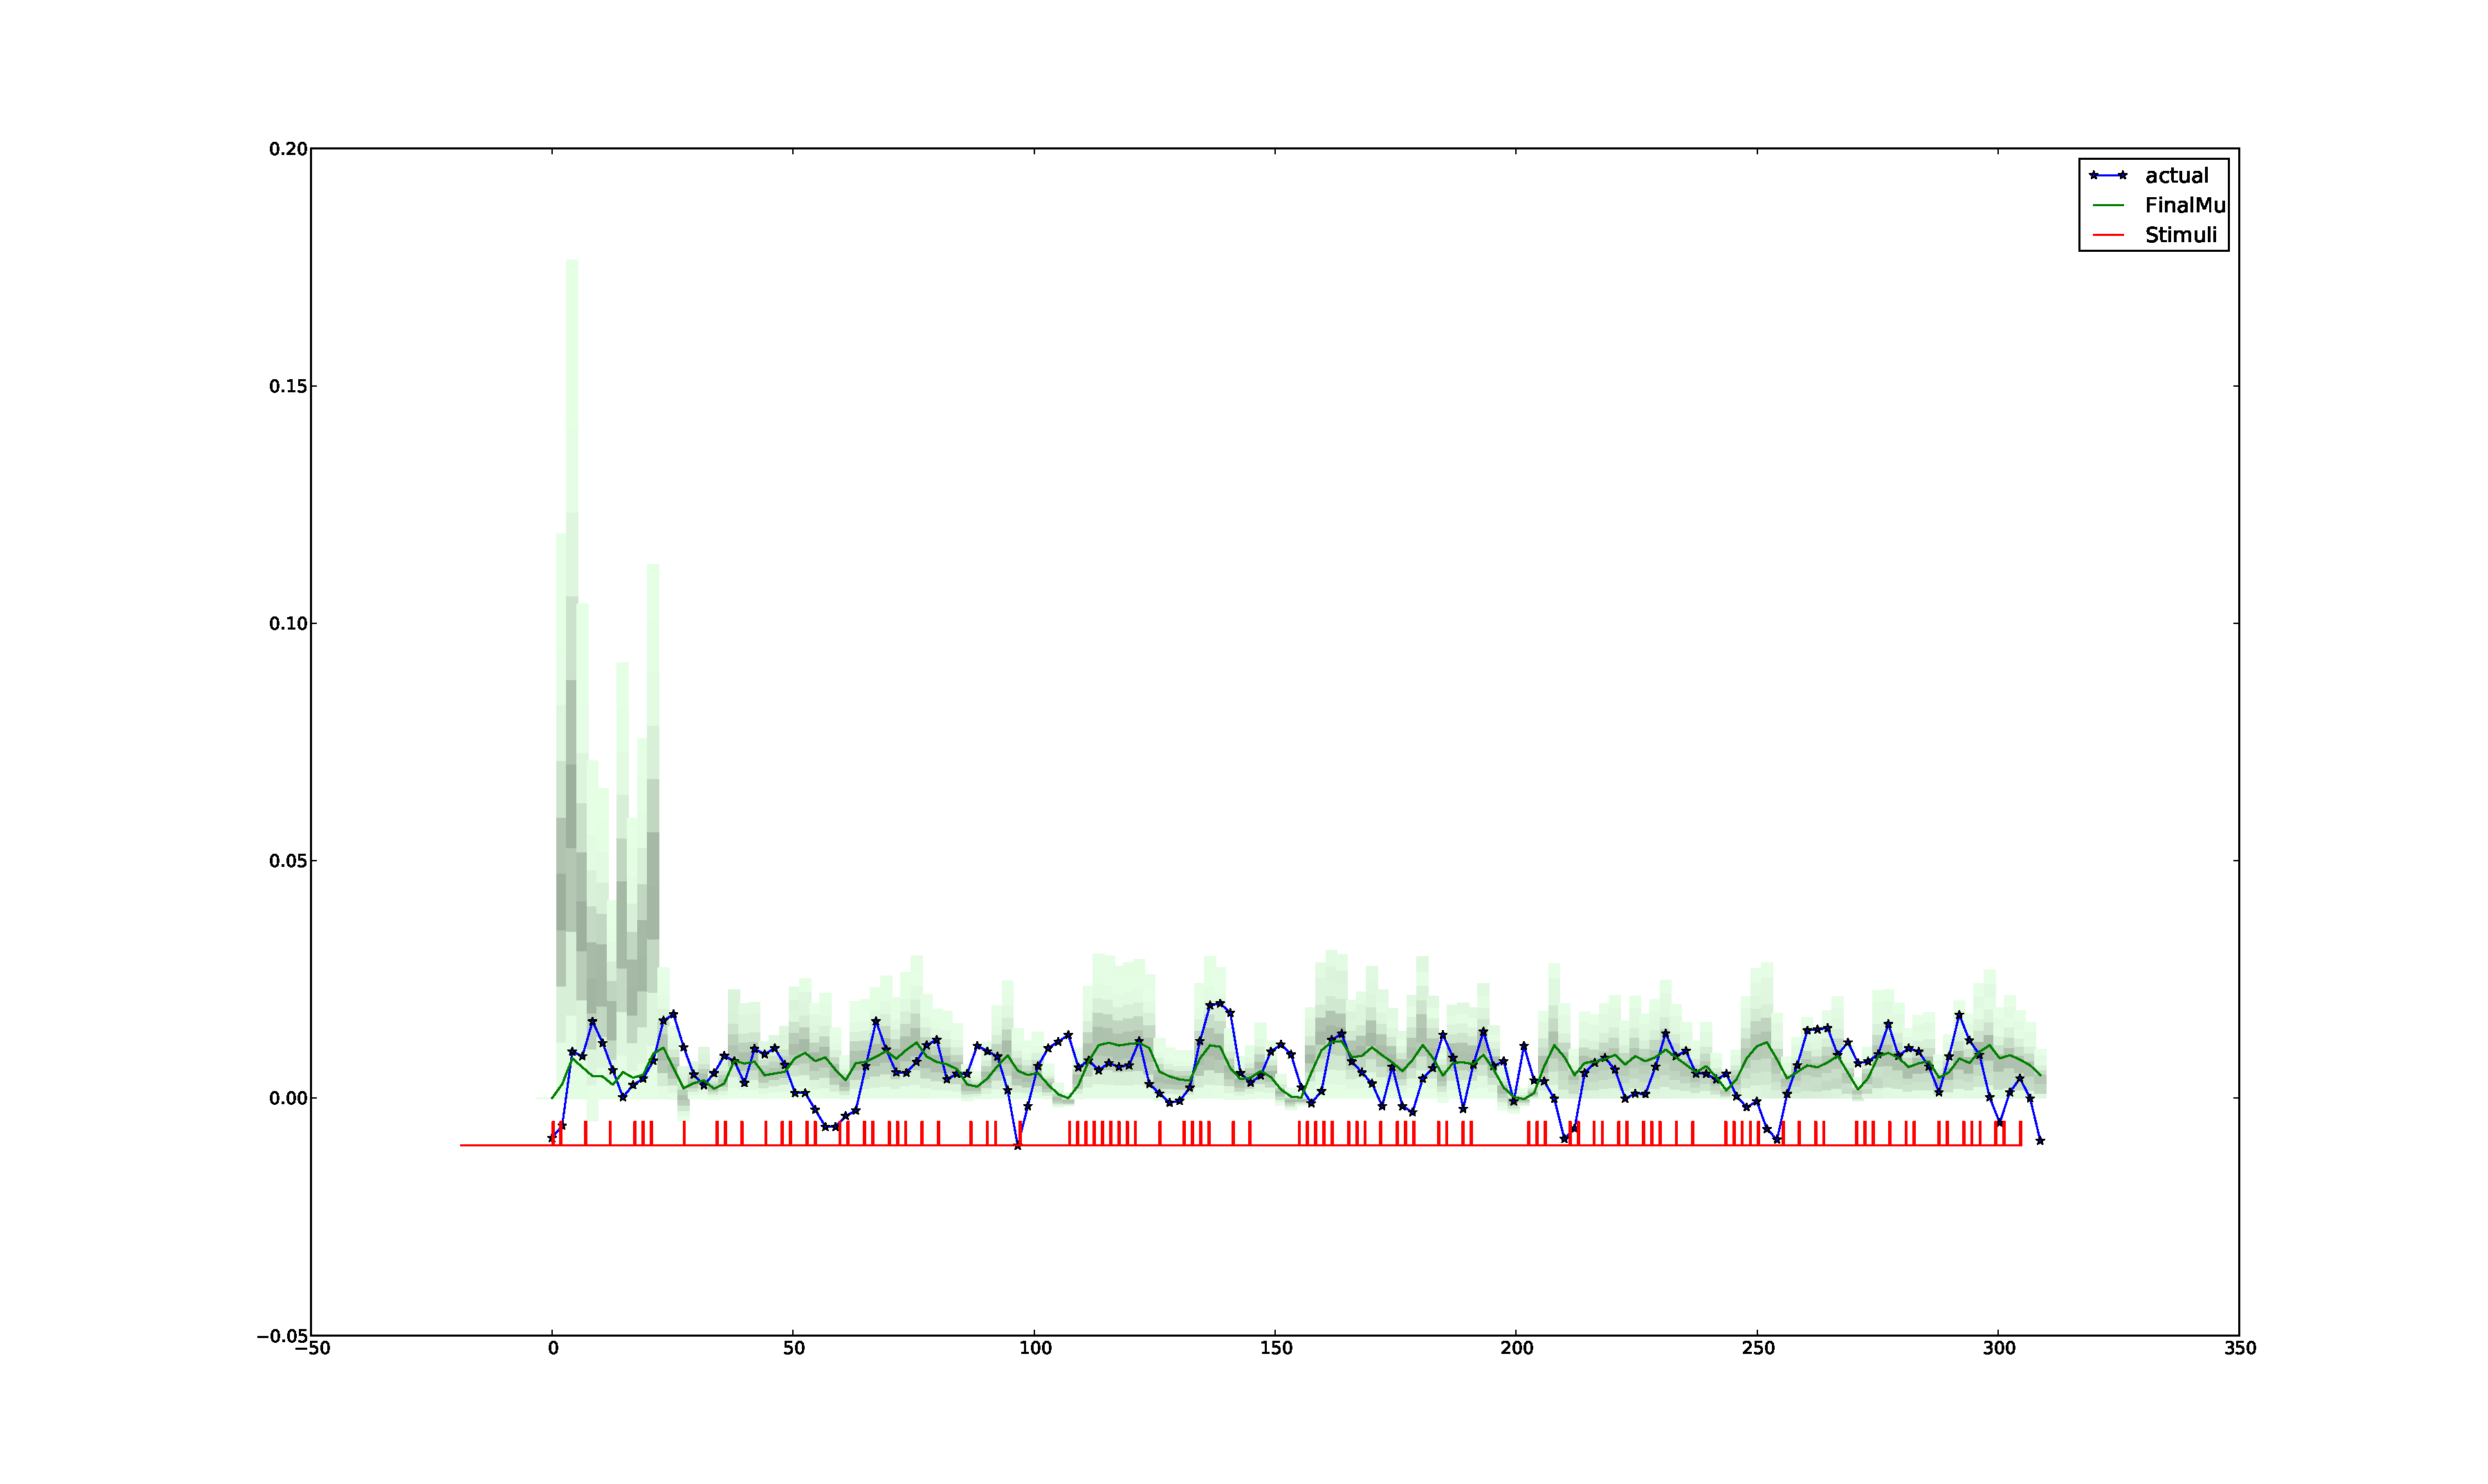
\includegraphics{images/param2a}}
\subfigure[]{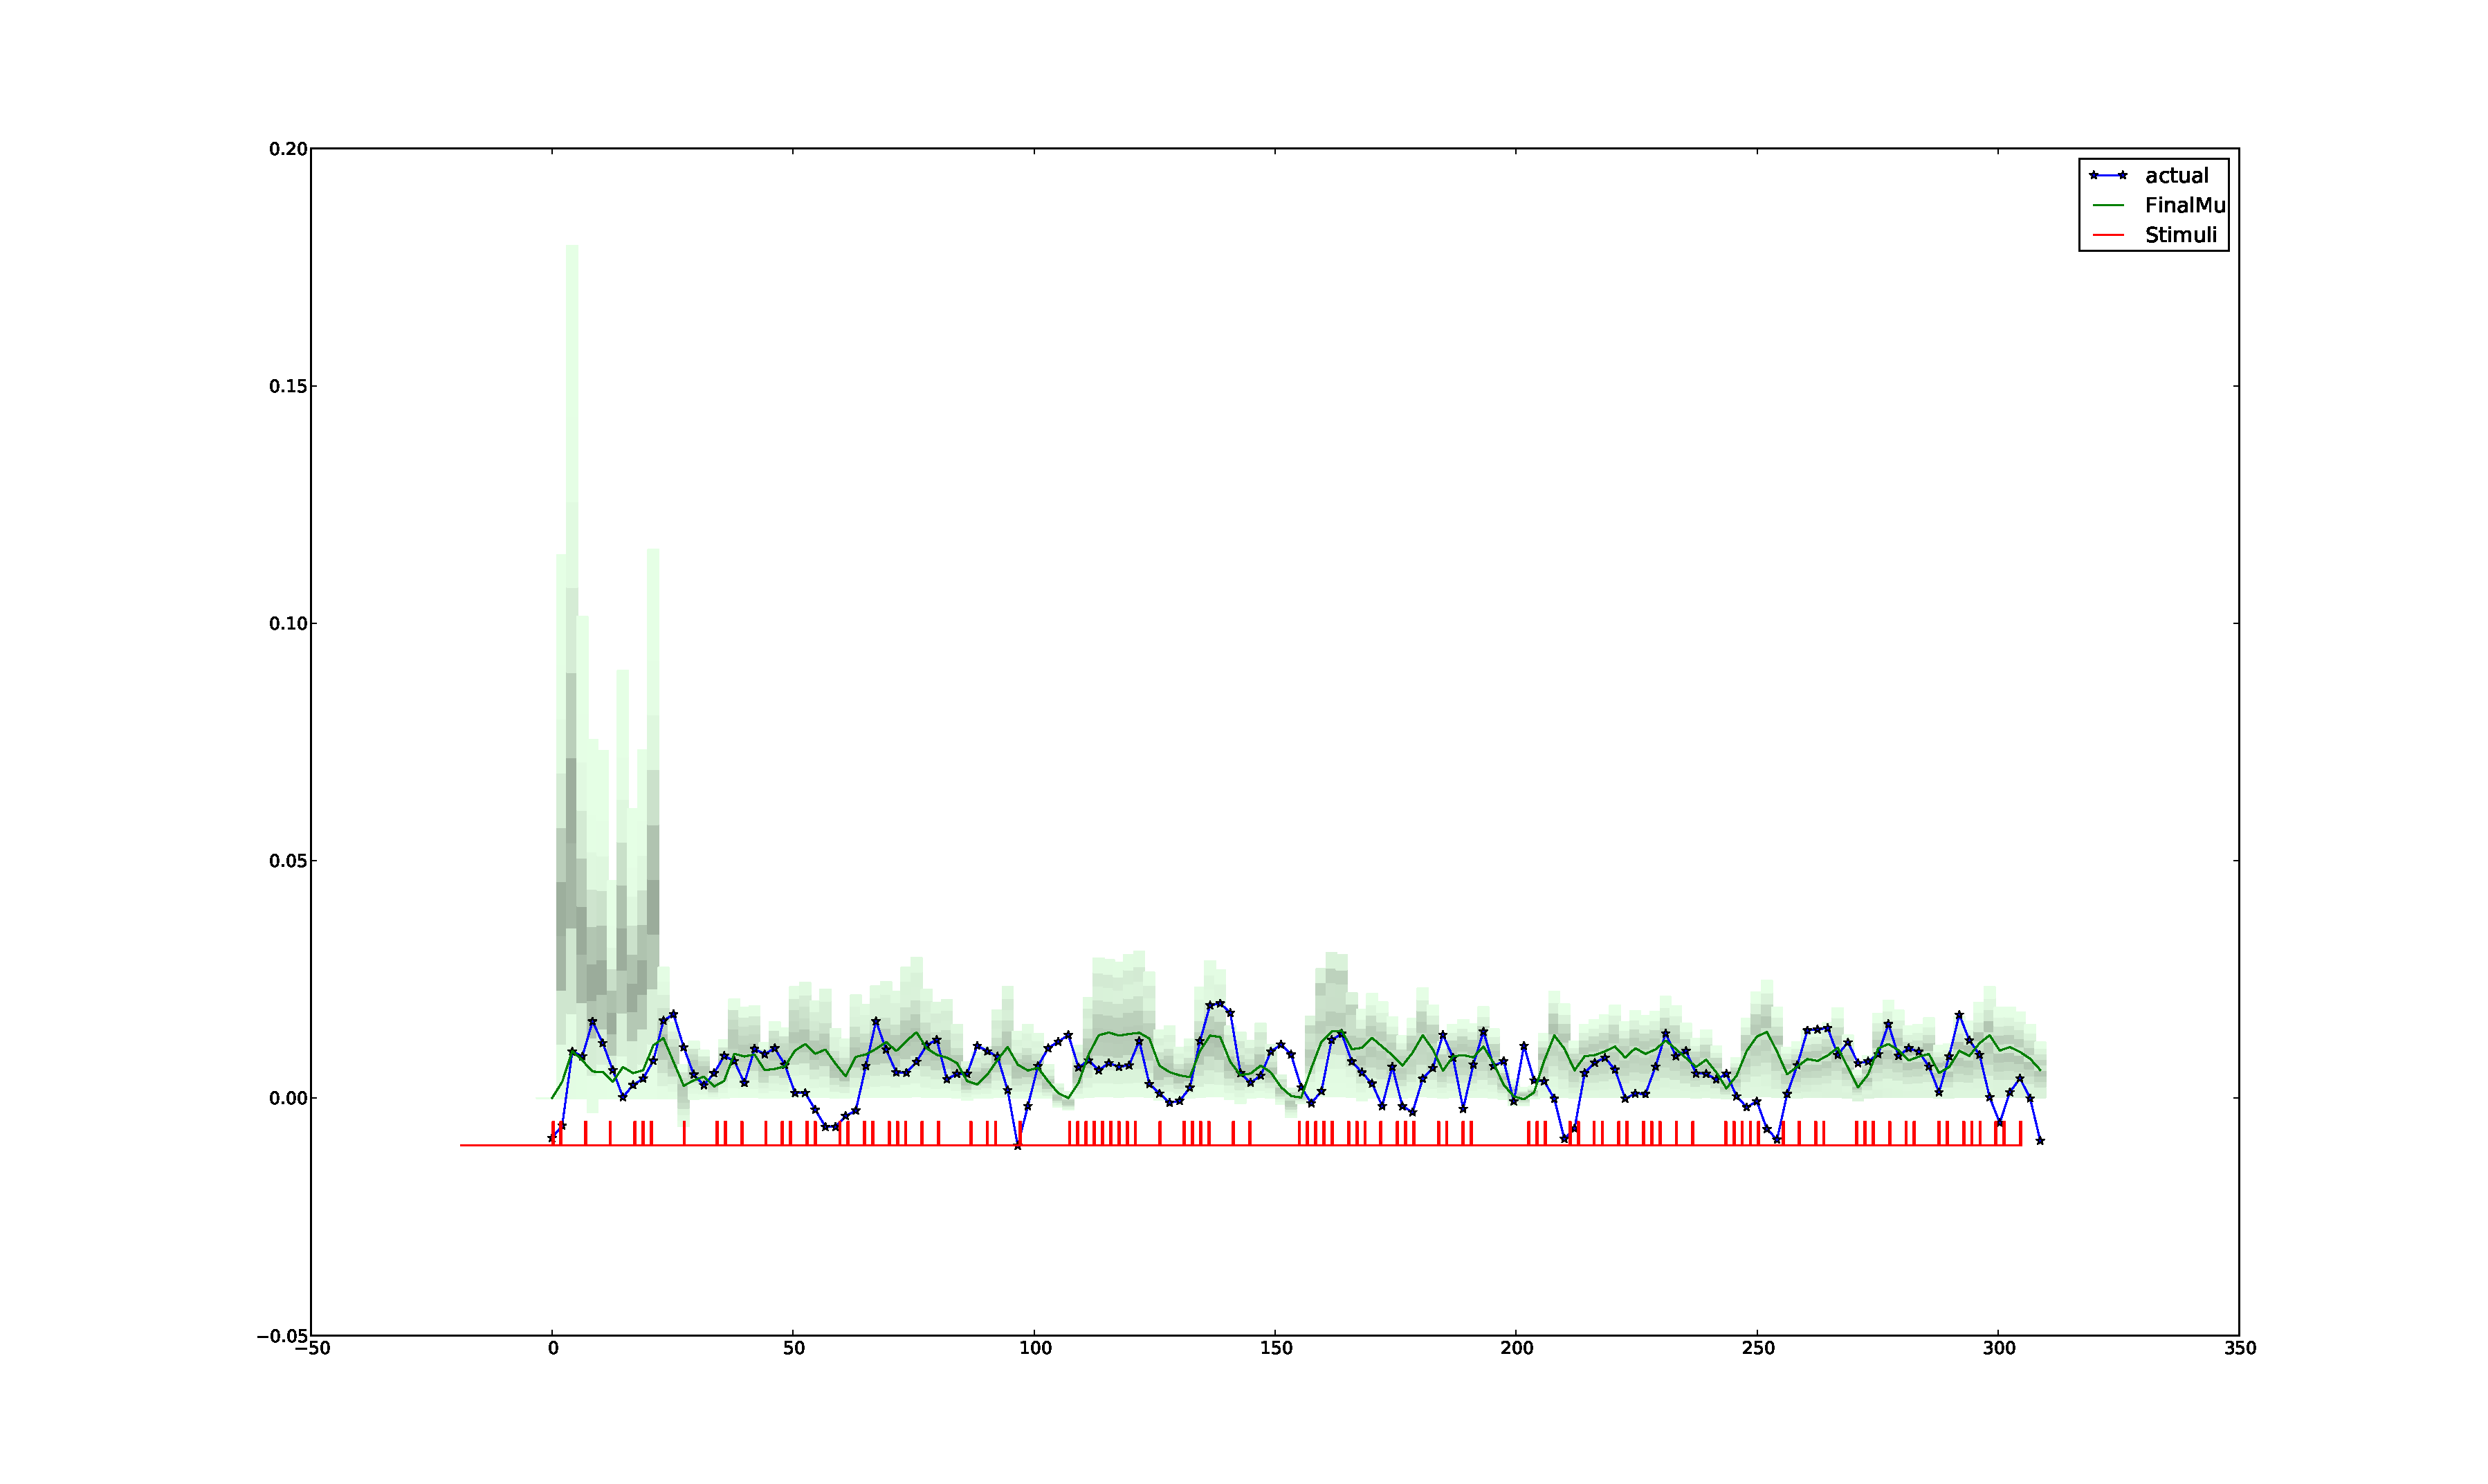
\includegraphics{images/param2b}}
\caption{A poor fit, using the same parameters as }
\end{figure}

\section{Particle Collapse Recovery}
This heuristic was initially intended to deal with cases where the particle
filter prematurely converged; and to reverse this effect. In reality, however
it did not perform well, and so it was not used in full-brain analysis. Ultimately
it did not prevent collapse of the distribution, and it often caused dramatic
increased in the variance of parameter estimates. It also pronged the analysis
time of inactive time series. Essentially the effect was exactly opposite of what
one would hope.


\section{Weighting Function Comparison}
\label{sec:Results Weights}

\section{Single Time-Series Simulation}

Graphs: 

For simulated data, single timeseries:

For \{delta, DC/Spline\}, \{exponential, gaussian, cauchy\}, \{biased, unbiased initial\},
\{100, 500, 1000\} particles
\begin{enumerate}
\item Ground truth vs. Estimated signal during particle filter run
\item Ground truth vs. Estimated signal with final parameter set
\item True Parameters vs. Final Parameter Sets
\item Variance of final parameters when faced with same ground truth, different noise
\item MSE of (a new timeseries based on X(t) vs. ground truth) for all t
\item Estimator Variance based on different noise runs
\item Final Particle Distribution
\end{enumerate}

For Simulated Data, Full Volume:

%note to self, epsilon should probably be uniform between 0 and something
\section{Simulated Volume}
\begin{enumerate}
\item Parameter Map 
\item Error map of parameters
\item Histogram of \%errors between parameters
\item Activation Map based on a single region with high $\epsilon$, compared with linear
\end{enumerate}

Final parameter distribution among active regions.
Q-Q plots?

\section{FMRI Data}
....

image comparing epsilon-map with GLM activation map


%\chapter{Real Data}
%Finally, we also performed inference on a real FMRI scan. The scanner we used...
%... more specifics...

% TODO include single?
%Before performing tests on a full image, I the particle filter
%on regions deemed active and inactive by statistical parametric mapping
%(SPM). This served the purpose of adjusting the priors as well as the 
%preprocessing based on real world signals. This was actually done before
%the simulations, and then results were carried back the simulations 
%to check consistency.
%After work adjusting parameters, most importantly the weighting function and the 
%priors, particle filter was applied to every voxel in an FMRI image.
%The results of this large scale analysis was a parameter map which was
%then used to calculate normalized square-root MSE image. 
%
%\section{Single-Voxel Analysis}
%The choice of a prior, as discussed previously, is extremely important. While a
%prior may have the potential to give good results, being a monte-carlo algorithm
%there is the possibility for inconsistencies. Thus, increasing the variance
%of the time-constants may allow additional flexibility, it will also cause
%additional model variance. Before running on a full volume I adjusted the 
%prior to ensure that the same input would give the same output 100 times in a 
%row. While this may seem like a given, with a random drawing of the prior,
%this can be difficult. Case in point, the exact same algorithm run twice
%with the time constants all having standard deviations of $.35$ resulted in two
%very different fits, shown in \autoref{fig:badfit_param1}.
%
%\begin{figure}
%\subfigure{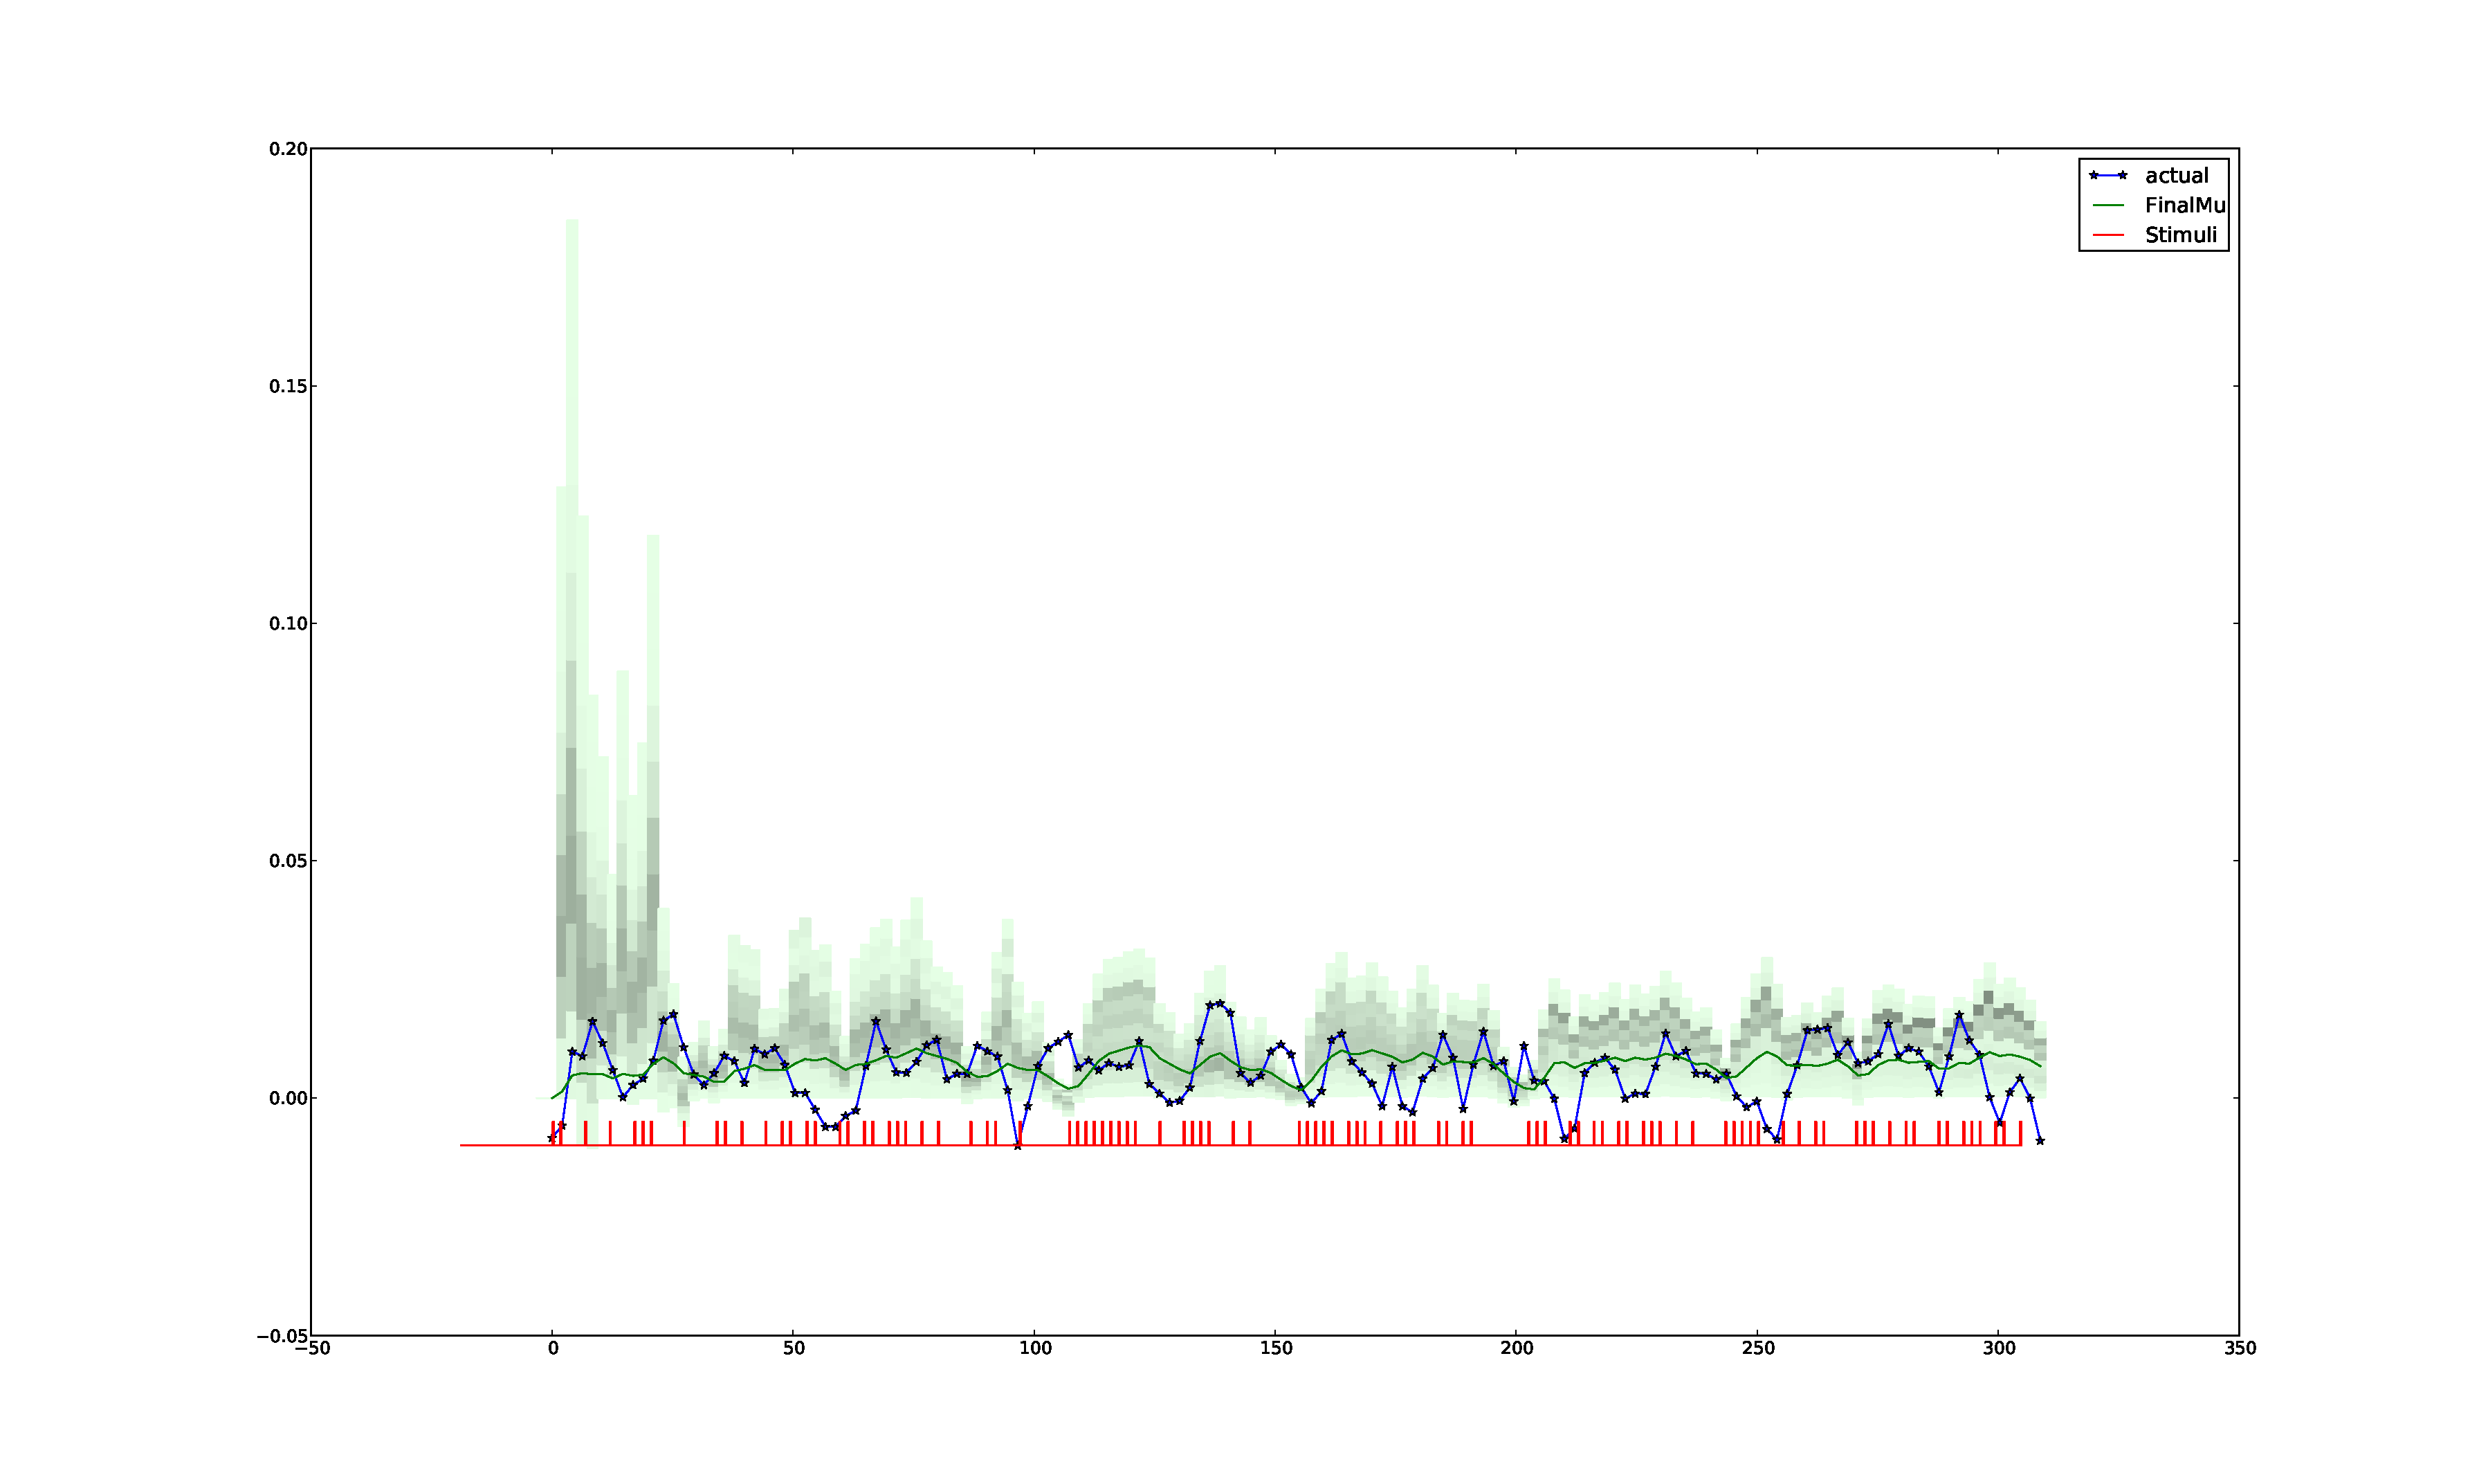
\includegraphics[clip=true,trim=6cm 2cm 6cm 3.5cm,width=17cm]{images/badfit_param1}}
%\subfigure{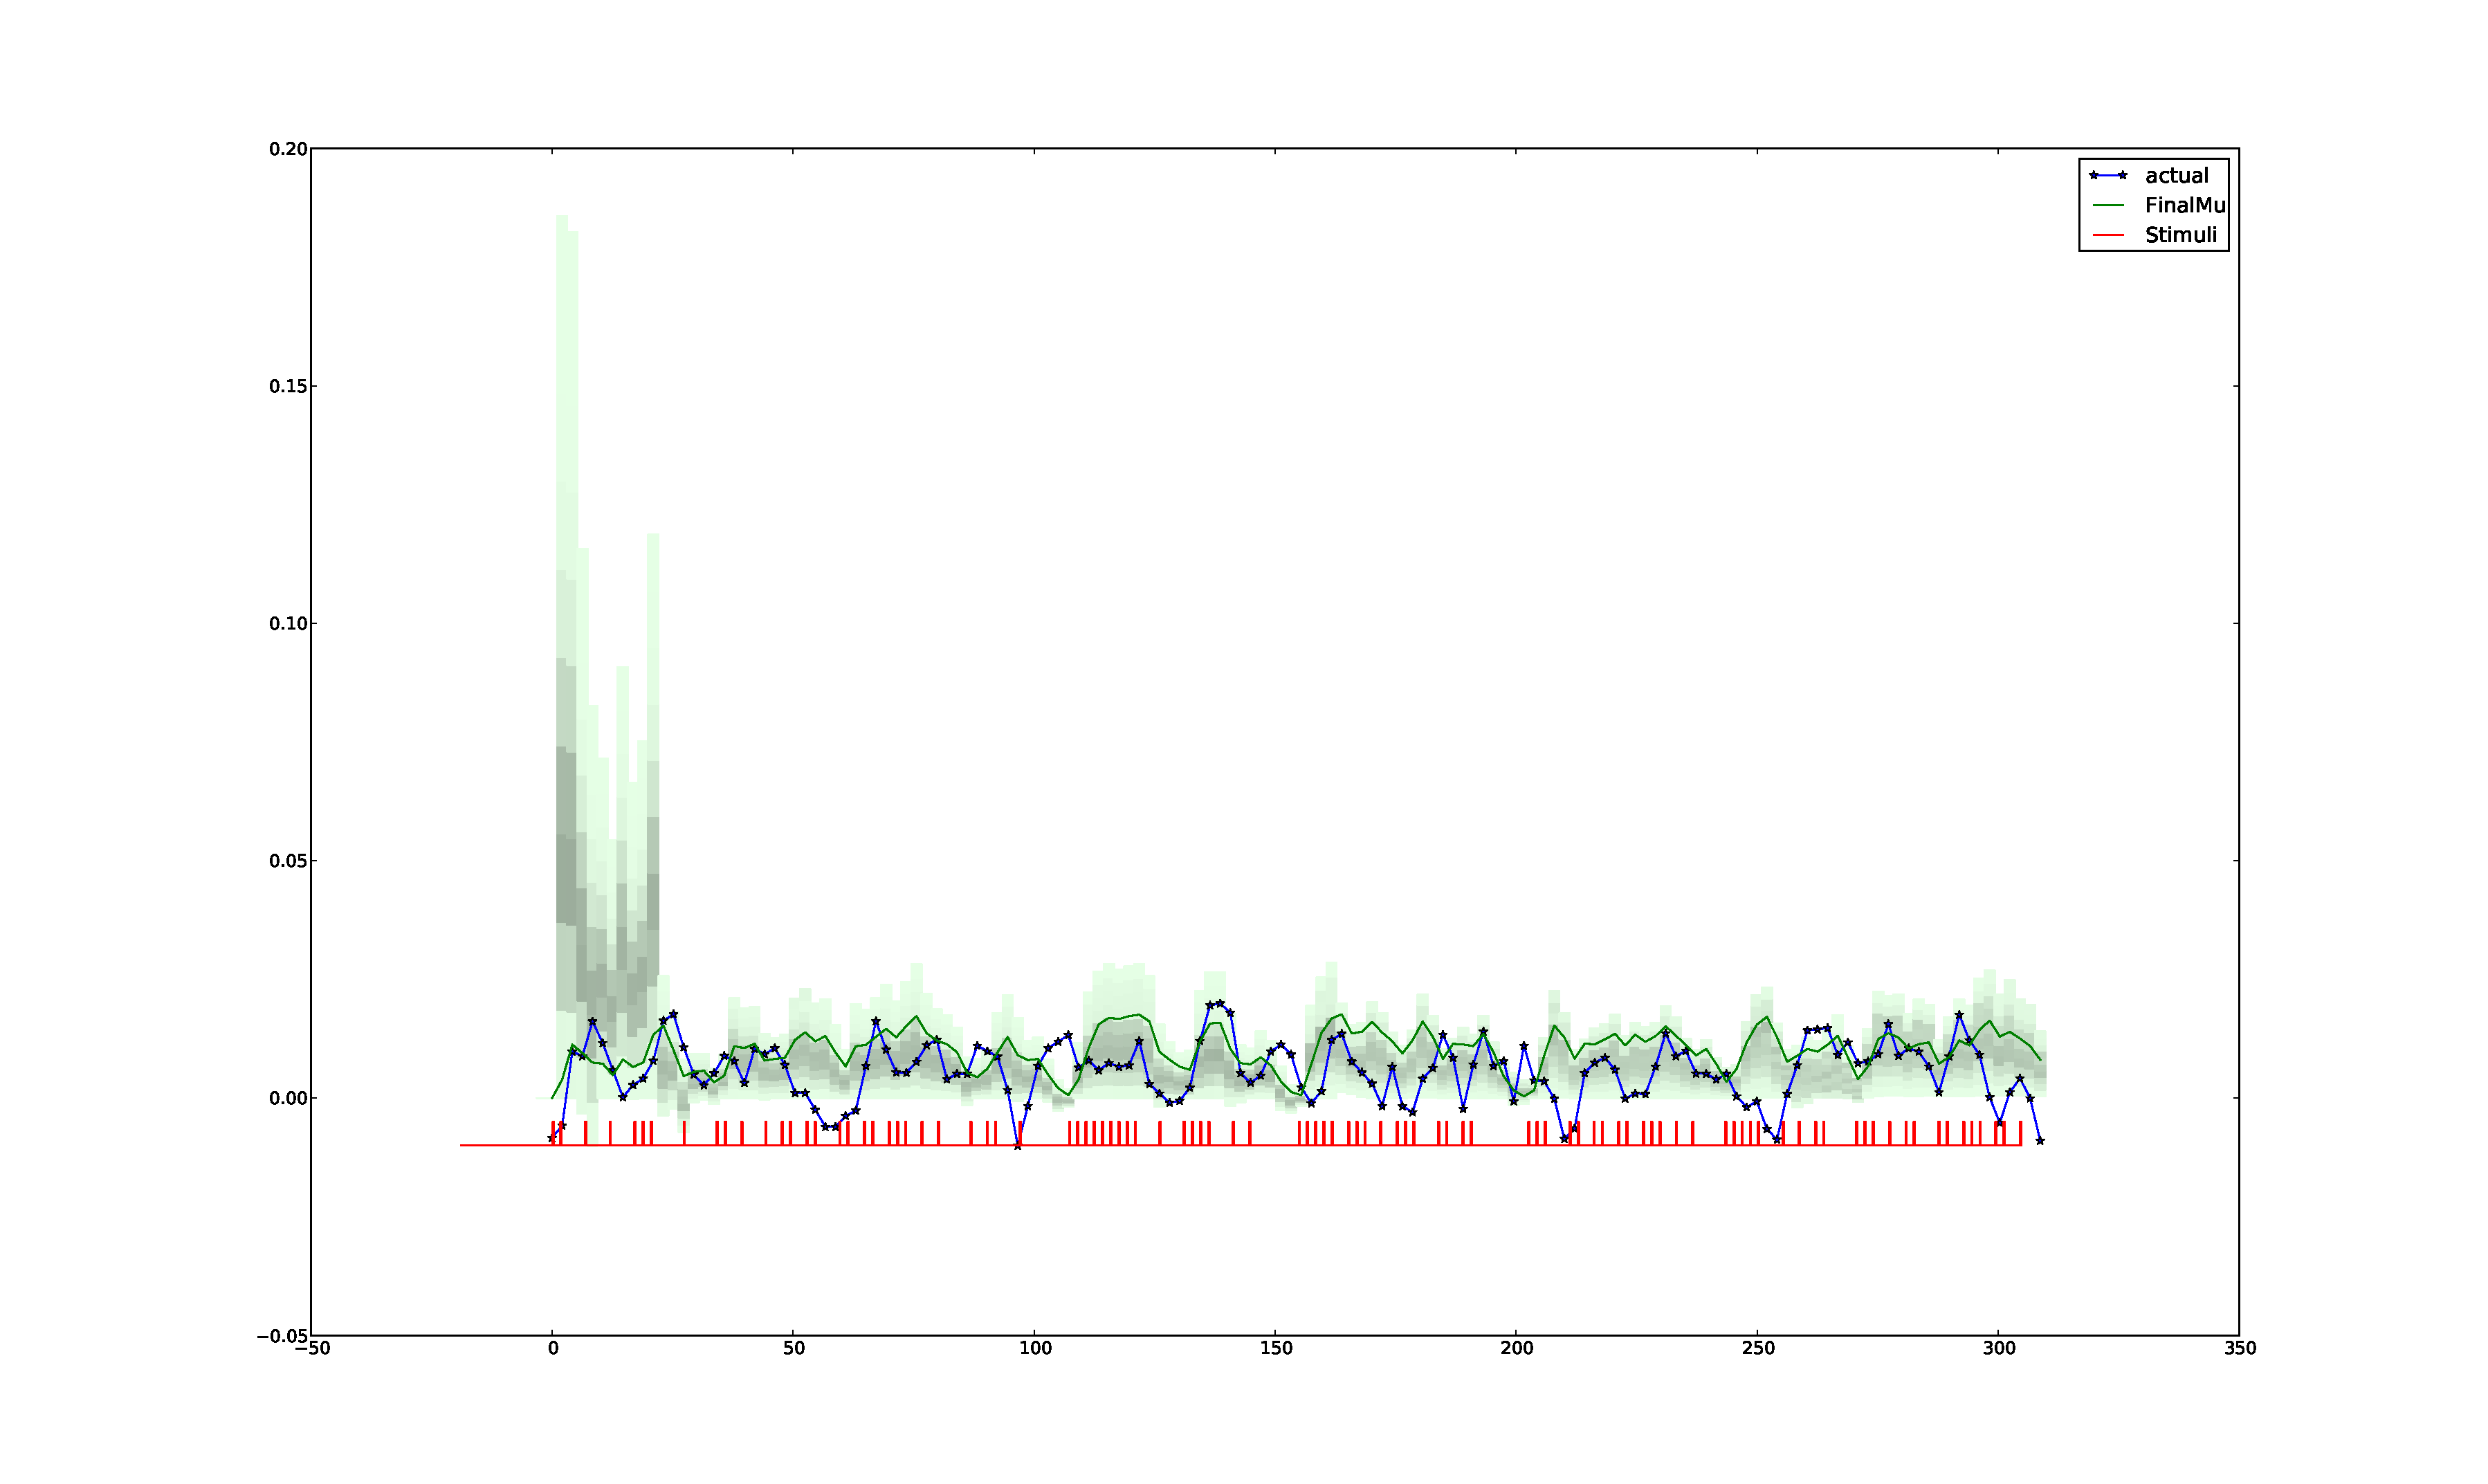
\includegraphics[clip=true,trim=6cm 2cm 6cm 3.5cm,width=17cm]{images/goodfit_param1}}
%\caption{The same priors gave rise to both fits.}
%\label{fig:badfit_param1}
%\end{figure}
%
%For this reason, I actually lowered the standard deviations of the time
%constants to prevent over-smoothing. This resulted in more consistent,
%though potentially slightly worse fits, two examples of which are 
%shown in \autoref{fig:param2_var}. 
%
%\begin{figure}
%\subfigure{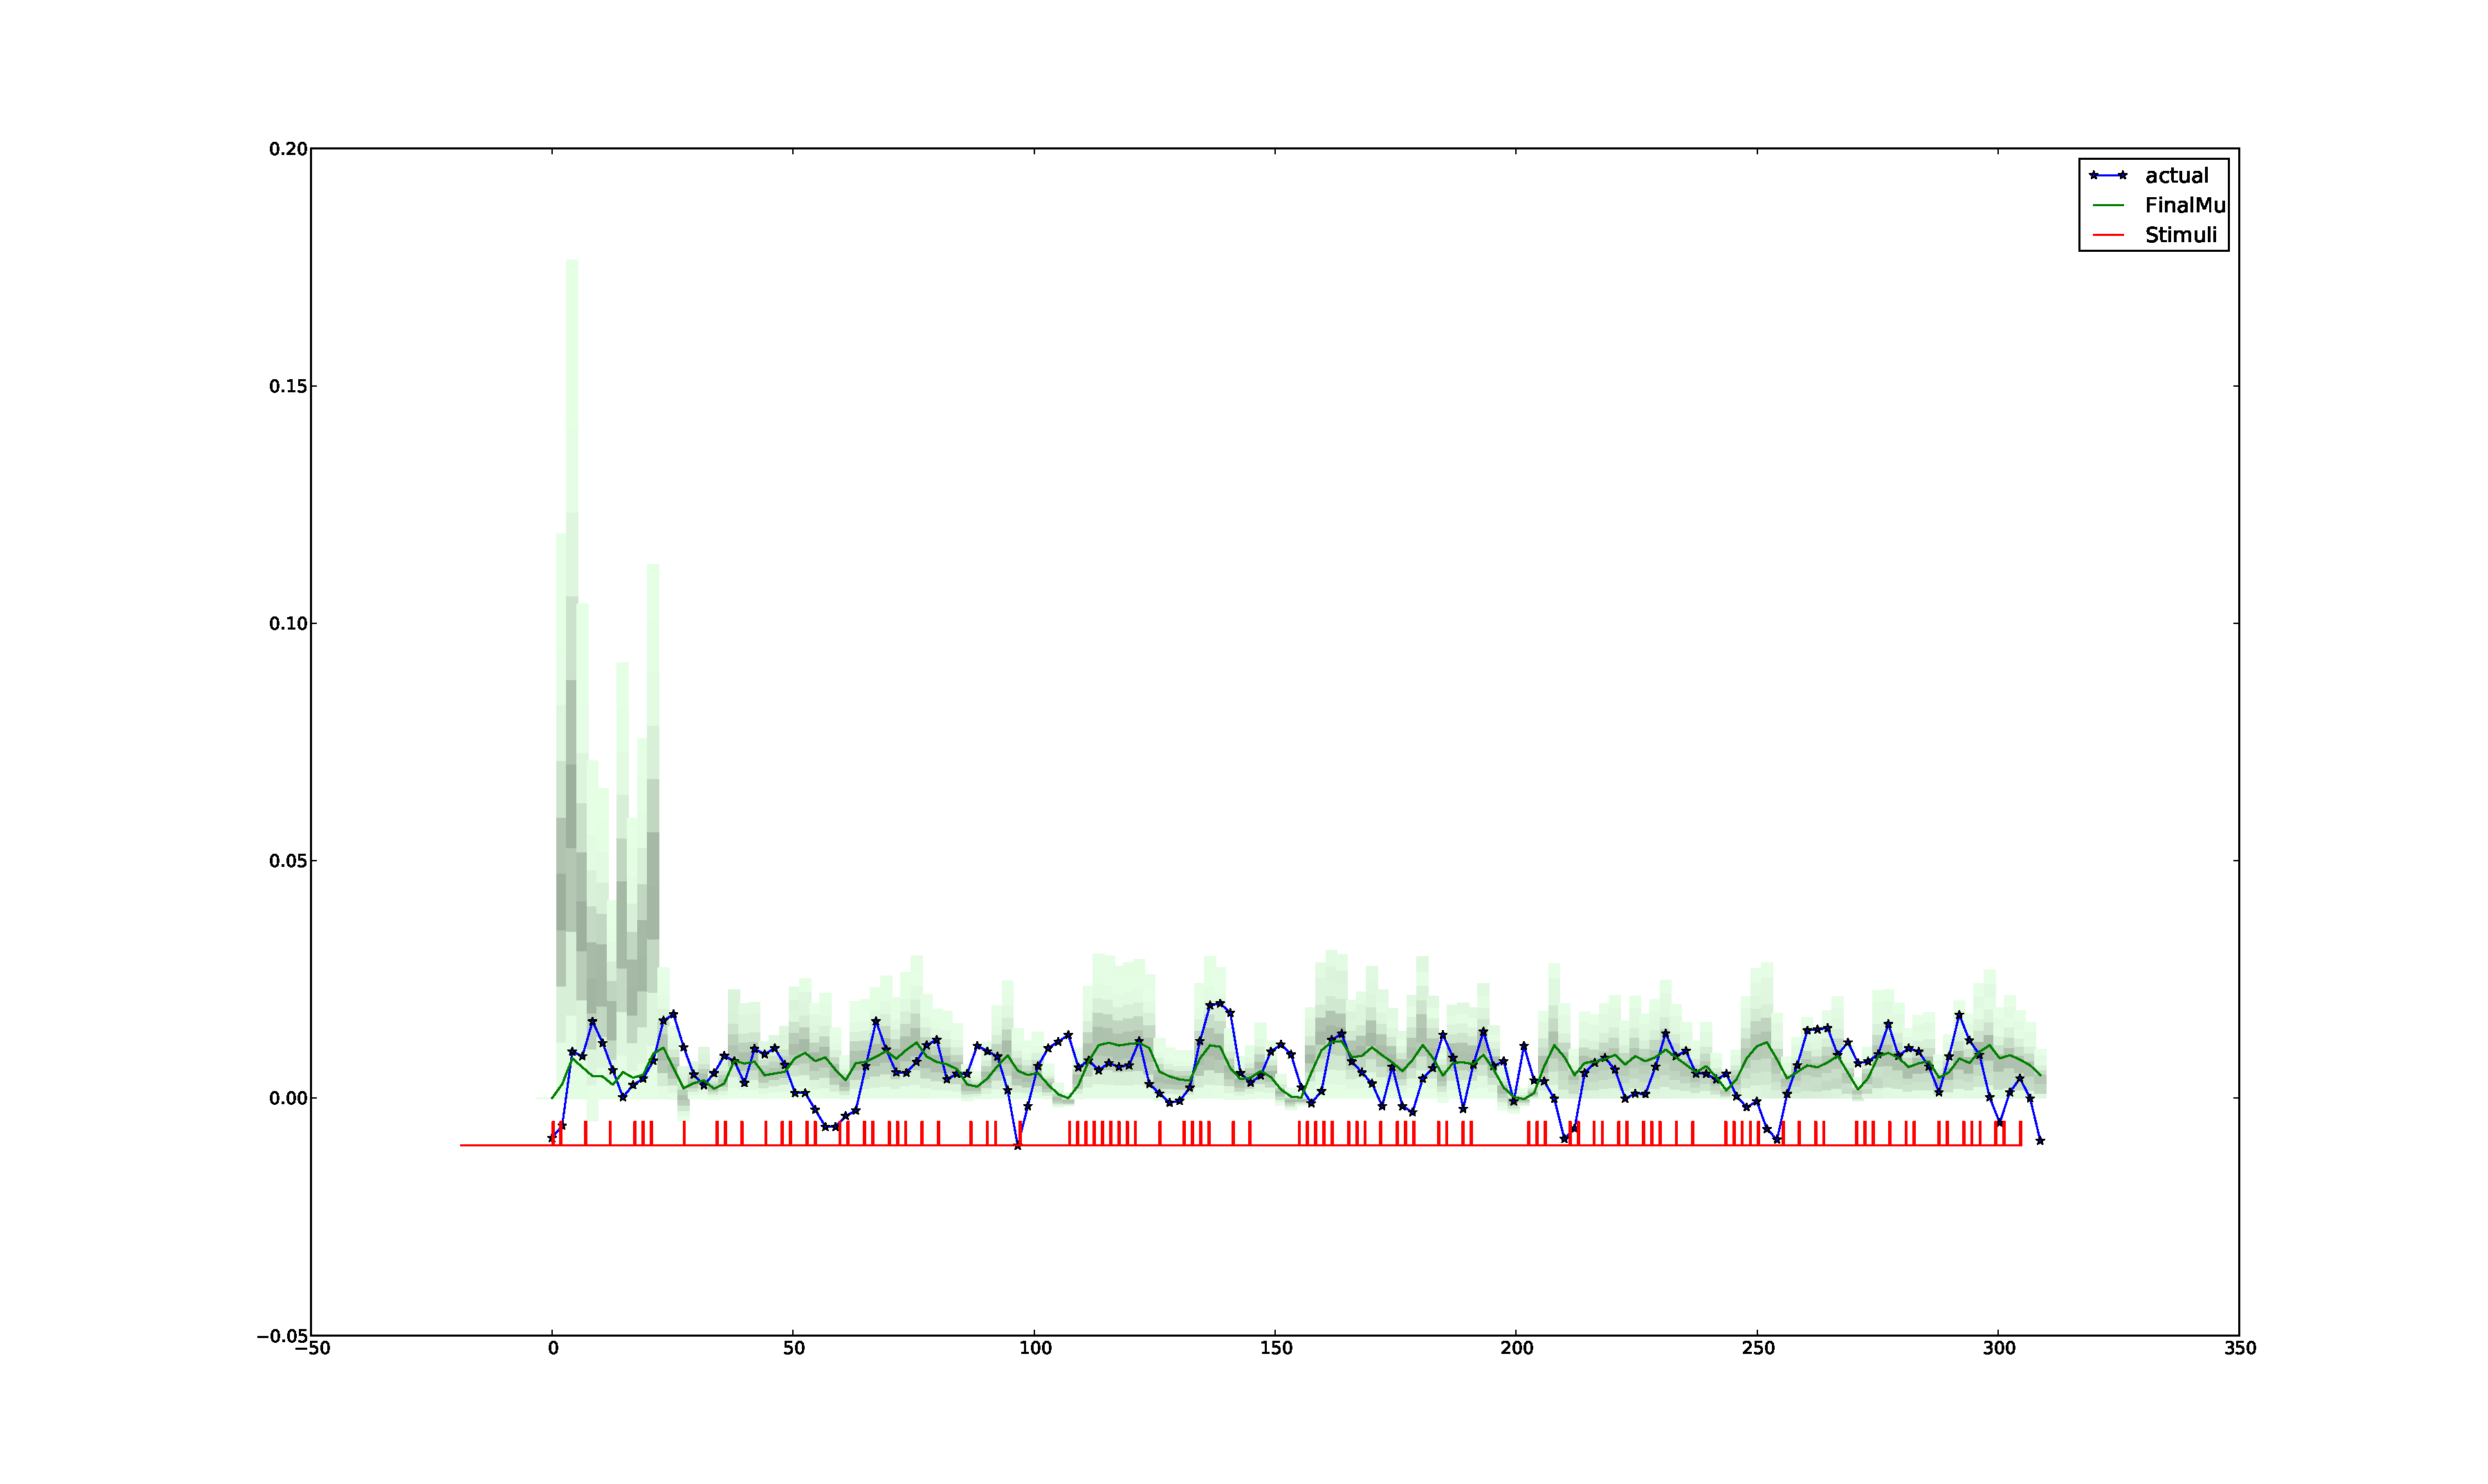
\includegraphics[clip=true,trim=6cm 2cm 6cm 3.5cm,width=17cm]{images/param2a}}
%\subfigure{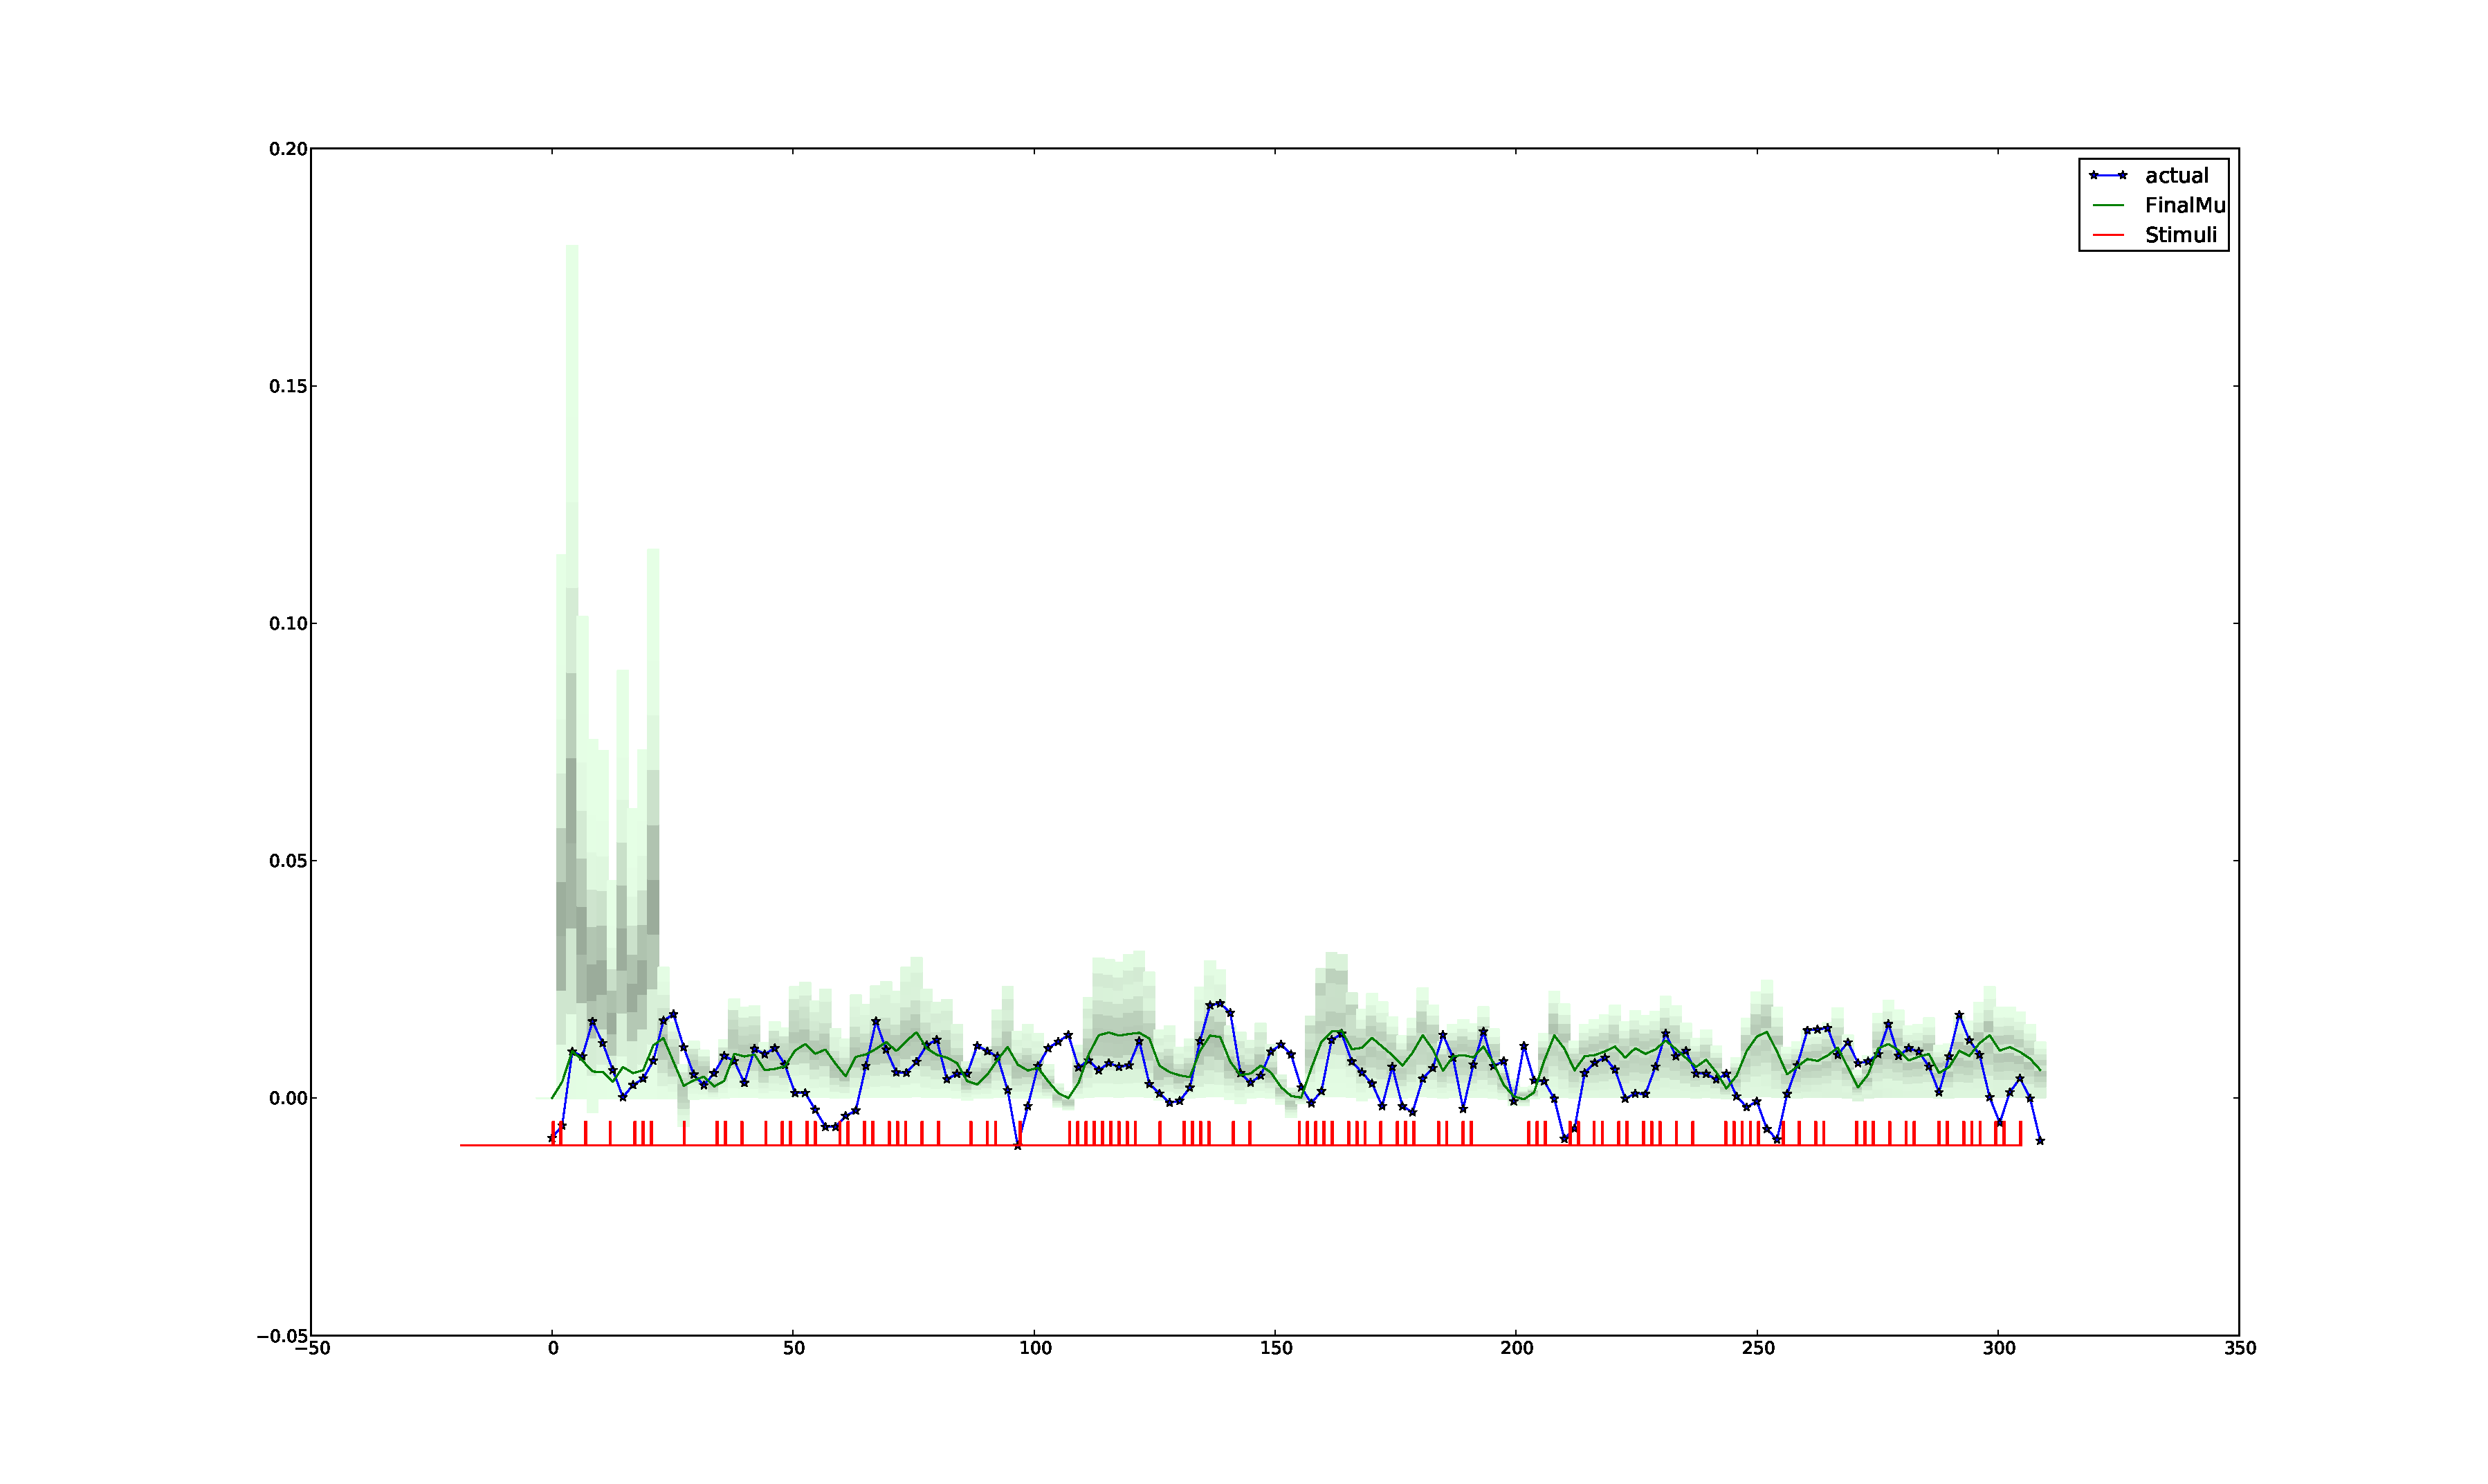
\includegraphics[clip=true,trim=6cm 2cm 6cm 3.5cm,width=17cm]{images/param2b}}
%\caption{A poor fit, using the same parameters as }
%\label{fig:param2_var}
%\end{figure}
%
%todo: stats of the 100 fits?
%
%\section{Single Time-Series Simulation}
%
\chapter{Real Data}
\label{sec:RealData}
Modeling the BOLD response is of course not of much use if does not work for
real FMRI.  Although this algorithm will hopefully lead to more novel methods 
of analysis, the standard use for modeling the BOLD signal is to locate activation.
Activation is defined as areas where the input is the primary drive
for the BOLD response, as opposed to intermediate factors controlling it. 
Once areas where the BOLD 
model may be accurately estimated are found, integrating the model will allow for accurate
estimation of the state between measurements, which could then be used for more 
advanced analysis, for instance of areas that are being driven by other brain regions.
It all begins with localizing the first activation regions in the
chain. Therefore this section compares the output of the particle filter 
with conventional SPM. 

The data described in this section are fundamentally different in several 
ways. SPM preprocesses the image by spatially smoothing the FMRI image (in this section 
SPM8 was used with an $8mm x 8mm x 8mm$ Gaussian kernel), whereas
this is not done in the particle filter algorithm. Additionally, a spline
was used to de-trend, rather than SPM8's high pass filter (with a cut
off based on a globally estimated autocorrelation). Thus the preprocessing pipelines 
are different; but the output of SPM8 is also different. Whereas SPM outputs
a t-statistic for each voxel, the output 
of the particle filter is a posterior probability distribution of the parameters
at every voxel. To validate the quality of the particle filter results 
it is necessary to compare the both the location and the fit calculated by the particle filter
with SPM's location and fit.

\section{Results}
The results from T-values from SPM8 are shown in \autoref{fig:hm_canon_spm} (threshold of
4), and the results from 
the particle filter are shown in \autoref{fig:hm_canon_pfilter} and \autoref{fig:hm_canon_pfilter_mi}.
Note that the scales for all three images are different, because the metrics are different.
SPM measures using T-Tests to determine the likelihood of a false positive. \autoref{fig:hm_canon_pfilter}
uses simple normalized residuals, meaning that lower indicates less error.  
\autoref{fig:hm_canon_pfilter_mi} measures in terms of the dependence between the 
measured signal and the estimated signal; thus higher indicates a better fit. The particle
filter data shows a large number of false positives, however application of a threshold
of $.85$ on the residual map removes these false positives. Similarly, in the mutual information
map, the false positives may be elminated by upping the threshold to $.15$. However, just
because the results disagree with SPM does not necessarily mean they are false positives.
SPM operates on smoothed data (8mm x 8mm x 8mm), so there are certainly active 
areas that have been missed because of the smoothing. 

\begin{figure}[H]
\subfigure[]{\label{fig:hm_spm} \includegraphics[scale=.85]{images/spm_hm}}
\subfigure[]{\label{fig:hm_canon_spm_x} \includegraphics[scale=3]{images/spm_hm_x}}
\subfigure[]{\label{fig:hm_canon_spm_y} \includegraphics[scale=3]{images/spm_hm_y}}
\subfigure[]{\label{fig:hm_canon_spm_z} \includegraphics[scale=3]{images/spm_hm_z}}
\subfigure{\label{fig:scale_spm} \includegraphics[scale=.5]{images/scale1}}
\caption{Sagittal, coronal and axial slices of SPM results (\autoref{fig:hm_canon_spm_x} \autoref{fig:hm_canon_spm_y} 
         \autoref{fig:hm_canon_spm_x}), as well as a series of axial slices, \autoref{fig:hm_spm}. Units
         of activation are in Student's T-scores. Higher indicates higher assurance that the signal cannot
         have occurred through noise alone.}
\label{fig:hm_canon_spm}
\end{figure}

\begin{figure}[H]
\subfigure[]{\label{fig:hm_pfilter} \includegraphics[scale=.85]{images/pfilter_hm}}
\subfigure[]{\label{fig:hm_canon_pfilter_x} \includegraphics[scale=3]{images/pfilter_hm_x}}
\subfigure[]{\label{fig:hm_canon_pfilter_y} \includegraphics[scale=3]{images/pfilter_hm_y}}
\subfigure[]{\label{fig:hm_canon_pfilter_z} \includegraphics[scale=3]{images/pfilter_hm_z}}
\subfigure{\label{fig:scale_pfilter} \includegraphics[scale=.5]{images/scale2}}
\caption{Sagittal, coronal and axial (\autoref{fig:hm_canon_pfilter_x} \autoref{fig:hm_canon_pfilter_y} 
         \autoref{fig:hm_canon_pfilter_x}), as well as a series of axial slices, \autoref{fig:hm_pfilter}. 
         Units of match is normalized residual. The lowest (best) levels were $.7$.
         The highest error shown is $1$.}
\label{fig:hm_canon_pfilter}
\end{figure}

%\begin{figure}[H]
%\subfigure[]{\label{fig:hm_pfilter85} \includegraphics[scale=.75]{images/pfilter85_hm}}
%\subfigure[]{\label{fig:hm_canon_pfilter85_x} \includegraphics[scale=3]{images/pfilter_hm85_x}}
%\subfigure[]{\label{fig:hm_canon_pfilter85_y} \includegraphics[scale=3]{images/pfilter_hm85_y}}
%\subfigure[]{\label{fig:hm_canon_pfilter85_z} \includegraphics[scale=3]{images/pfilter_hm85_z}}
%\subfigure{\label{fig:scale_pfilter85} \includegraphics[scale=.5]{images/scale3}}
%\caption{Sagittal, coronal and axial (\autoref{fig:hm_canon_pfilter_x} \autoref{fig:hm_canon_pfilter_y} 
%         \autoref{fig:hm_canon_pfilter_x}), as well as a series of axial slices, \autoref{fig:hm_pfilter}. 
%         Units of match is normalized residual. The lowest (best) levels were $.7$.
%         The highest error shown is $.85$.}
%\label{fig:hm_canon_pfilter85}
%\end{figure}

\begin{figure}[H]
\subfigure[]{\label{fig:hm_mi} \includegraphics[scale=.85]{images/mi_hm}}
\subfigure[]{\label{fig:hm_canon_mi_x} \includegraphics[scale=3]{images/mi_hm_x}}
\subfigure[]{\label{fig:hm_canon_mi_y} \includegraphics[scale=3]{images/mi_hm_y}}
\subfigure[]{\label{fig:hm_canon_mi_z} \includegraphics[scale=3]{images/mi_hm_z}}
\subfigure{\label{fig:scale_mi} \includegraphics[scale=.5]{images/scale4}}
\caption{Sagittal, coronal and axial (\autoref{fig:hm_canon_pfilter_x} \autoref{fig:hm_canon_pfilter_y} 
         \autoref{fig:hm_canon_pfilter_x}), as well as a series of axial slices, \autoref{fig:hm_pfilter}. 
         Units of match is bits (standard for base-2 Mutual Information). The highest (best) levels are 
         $.42$. The worst shown is $.1$.}
\label{fig:hm_canon_pfilter_mi}
\end{figure}

\begin{figure}
\subfigure[Particle Filter]{\label{fig:comp1pfilter} \includegraphics[clip=true,trim=5cm 1cm 4cm 1cm,width=15cm]{images/1_pfilter_37_14_7}}\\
\subfigure[SPM]{\label{fig:comp1spm} \includegraphics[clip=true,trim=5cm 1cm 4cm 1cm,width=15cm]{images/1_spm_37_14_7}}
\caption{Section 1, Estimated vs. Actual BOLD response}
\label{fig:comp1}
\end{figure}

 
\begin{figure}
\subfigure[Particle Filter]{\label{fig:comp2pfilter} \includegraphics[clip=true,trim=5cm 1cm 4cm 1cm,width=15cm]{images/2_pfilter_34_12_7}}\\
\subfigure[SPM]{\label{fig:comp2spm} \includegraphics[clip=true,trim=5cm 1cm 4cm 1cm,width=15cm]{images/2_spm_34_12_7}}
\caption{Section 2, Estimated vs. Actual BOLD response}
\label{fig:comp2}
\end{figure}

I chose several voxels to discuss further from \autoref{fig:hm_canon_pfilter} and \autoref{fig:hm_canon_spm}.
The first voxel, labeled 1, had a very high T-score, high mutual information,  as well as 
a low error (around $.7$). Thus, the
fit should be very good in both the SPM and particle filter output; this comparison is shown in 
\autoref{fig:comp1}. Recall that SPM worked on a slightly less noisy time series because of the
spatial smoothing; this explains the lack of the sharp peak in the particle filter's preprocessed
data. Regardless, as expected, both work. 

I chose the second voxel (\autoref{fig:comp2}) because it was active in SPM and it would appear to be in a prime
location to be active in the SPM image (given the results in the surrounding voxels). The fit,
however shows just why the residual was high and the mutual information was low. This is a
prime example of a false positive due to the large smoothing kernel applied by SPM. 
For instance at 75 seconds, the stimulus is not present, and so the signal should drop off; yet
it doesn't. While a few peaks seem to match, most of the signal does not correlate with the
expected state progression. This voxel is not being driven direcly by the input, although it
may be gated or driven through intermediate region. 

The third voxel, compared in \autoref{fig:comp3}, was far away from any other active voxels 
and yet had a very low (around $.7$) residual. At the same time, the mutual information was
high enough to make the point suspect. Although the estimated signal seems to run down the
middle of the measurement signal; it is clear that there is a significant amount of noise
present in the signal that is not being explained by the particle filter, 
In both preprocessed time-series the input is extremely noisy, yet by the normalized residual 
the response is good. This is an example of a false positive from the residual metric. 

The fourth voxel (\autoref{fig:comp4}selected for anyalysis had a relatively high residual, and was not picked
for activation by SPM. On the other hand, the mutual information was above the threshold
for the image (todo). It is simple to see why the residual was not acceptable in this case.
At the same time, the peaks do seem to correlate with the measurement peaks. Regardless,
this is an example of a  false positive from the mutual information metric. 

The fifth voxel (\autoref{fig:comp5}) is an example of a region with increased activation
due to smoothing. The fit provided by the BOLD particle filter is not very good, and the time
series input to SPM is far less noisy. Regardless this is another case where the peaks
seem to match, yet nothing else does. Take for instance the measurements from $30$ seconds
to $40$ seconds. At that point there is a significant spike in the BOLD signal, yet the
actual measured signal declines. This is an indication that the BOLD signal is not directly
being driven by the input. It is likeley that the cause of the activation in this reason is
not true activation, but recieved from surrounding active regions through spatial smoothing. 

\begin{figure}
\subfigure[Particle Filter]{\label{fig:comp3pfilter} \includegraphics[clip=true,trim=5cm 1cm 4cm 1cm,width=15cm]{images/3_pfilter_23_21_7}}\\
\subfigure[SPM]{\label{fig:comp3spm} \includegraphics[clip=true,trim=5cm 1cm 4cm 1cm,width=15cm]{images/3_spm_23_21_7}}
\caption{Section 3, Estimated vs. Actual BOLD response}
\label{fig:comp3}
\end{figure}

\begin{figure}[H]
\subfigure[Particle Filter]{\label{fig:comp4pfilter} \includegraphics[clip=true,trim=5cm 1cm 4cm 1cm,width=15cm]{images/4_pfilter_26_15_7}}\\
\subfigure[SPM]{\label{fig:comp4spm} \includegraphics[clip=true,trim=5cm 1cm 4cm 1cm,width=15cm]{images/4_spm_26_15_7}}
\caption{Section 4, Estimated vs. Actual BOLD response}
\label{fig:comp4}
\end{figure}

% or in original coordinates 29-9-13
\begin{figure}
\subfigure[Particle Filter]{\label{fig:comp5pfilter} \includegraphics[clip=true,trim=5cm 1cm 4cm 1cm,width=15cm]{images/5_pfilter_29_9_13}}\\
\subfigure[SPM]{\label{fig:comp5spm} \includegraphics[clip=true,trim=5cm 1cm 4cm 1cm,width=15cm]{images/5_spm_29_9_13}}
\caption{Section 5, Below threshold in both particle filter checks, but above threshold in SPM. Mutual Information of $0.0212822$, T-Value
of $4.17399$ and $MSE$ of $1.14171$.}
\label{fig:comp5}
\end{figure}

%23-10-18 or in original coordinates 36-17-19
\begin{figure}
\subfigure[Particle Filter]{\label{fig:comp5pfilter} \includegraphics[clip=true,trim=5cm 1cm 4cm 1cm,width=15cm]{images/6_pfilter_36_17_19}}\\
\subfigure[SPM]{\label{fig:comp5spm} \includegraphics[clip=true,trim=5cm 1cm 4cm 1cm,width=15cm]{images/6_spm_36_17_19}}
\caption{Section 6, MI of $0.335504$, T Value: $2.49154$, normalized error: $0.783348$ Not visible in SPM}
\label{fig:comp6}
\end{figure}

%16-19-0 or in original coordinates 29-26-1
\begin{figure}
\subfigure[Particle Filter]{\label{fig:comp5pfilter} \includegraphics[clip=true,trim=5cm 1cm 4cm 1cm,width=15cm]{images/7_pfilter_29_26_1}}\\
%\subfigure[SPM]{\label{fig:comp5spm} \includegraphics[clip=true,trim=5cm 1cm 4cm 1cm,width=15cm]{images/5_spm_25_34_25}}
\caption{Section 7, $.1052$ in MI, $1.31534$ in SPM (which left this flat) and $1.09992$ normalized $\sqrt{MSE}$. Only visible in MI map. }
\label{fig:comp7}
\end{figure}

Voxel 6 (\autoref{comp6}) is another region that is active according to both metrics used
in this work, yet was missed by SPM. The time series in \autoref{comp6} shows an extremely
good fit, perhaps the best in this batch, for the particle filter. In contrast, the
fit for SPM is abysmal. In spite of the fact that several other areas around are active
as well, the smoothing seems to have completely wiped out activation in this voxel. 

Finally voxel 7 is a completely ambiguous time series. While the thresholds applied here
are empirical, this voxel is on the borderline of the thresholds for both mutual information
and the residual. The signal itself is extremely noisy, it should the voxel should be rejected.
However this case is reminiscent of the pure-noise tests performed in the previous chapter. 
This time series an extremely good example of the danger of false positives. In spite of the
fact that the signal oscillates far faster than the BOLD estimate, because of that, it is somehow
able to maintain a mutual information value of $.1052$ and a residual of just $1.09992$.
As such, a clear method of detecting these sorts of regions is necessary if the results
of the particle filter algorithm are toe be trusted. 

\section{Parameter Estimates}
Although the parameters are not uniquely identifiable by a single time-series, that
does not mean estimating them is not without benefit. The parameters still contain useful
information about the system. Additionally, as an aggregate they form a distribution of
the feasible parameters parameters for a particular patient. Therefore \autoref{fig:parammaps}
contains the parameter maps for the system and \autoref{} is a histogram across all voxels
for which the mutual information was greater than $.15$. As before, the threshold is not
scientifically derived, yet in tests this threshold provided a decent balance to remove most
of the questionably active voxels in the system. 

\begin{figure}[H]
\centering
\subfigure{\includegraphics[width=13cm]{images/pmap0}}
\subfigure{\includegraphics[scale=.5]{images/pscale_00}}
\caption{$\tau_0$ Estimates}
\end{figure}

\begin{figure}[H]
\centering
\subfigure{\includegraphics[width=13cm]{images/pmap1}}
\subfigure{\includegraphics[scale=.5]{images/pscale_01}}
\caption{$\alpha$ Estimates}
\end{figure}

\begin{figure}[H]
\centering
\subfigure{\includegraphics[width=13cm]{images/pmap2}}
\subfigure{\includegraphics[scale=.5]{images/pscale_02}}
\caption{$E_0$ Estimates}
\end{figure}

\begin{figure}[H]
\centering
\subfigure{\includegraphics[width=13cm]{images/pmap3}}
\subfigure{\includegraphics[scale=.5]{images/pscale_03}}
\caption{$V_0$ Estimates}
\end{figure}

\begin{figure}[H]
\centering
\subfigure{\includegraphics[width=13cm]{images/pmap4}}
\subfigure{\includegraphics[scale=.5]{images/pscale_04}}
\caption{$\tau_f$ Estimates}
\end{figure}

\begin{figure}[H]
\centering
\subfigure{\includegraphics[width=13cm]{images/pmap5}}
\subfigure{\includegraphics[scale=.5]{images/pscale_05}}
\caption{$\tau_s$ Estimates}
\end{figure}

\begin{figure}[H]
\centering
\subfigure{\includegraphics[width=13cm]{images/pmap6}}
\subfigure{\includegraphics[scale=.5]{images/pscale_06}}
\caption{$\epsilon$ Estimates}
\end{figure}

Regions with poor fit cannot have reliable parameter estimates because the input did not meaningfully
correlate input with output. Therefore before creating the maps,
each parameters map was masked to regions with mutual information greater than $.15$. I chose mutual
information over the residual because in the maps comparing regression fitness, the mutual information
maps had more coherency and less randomness. Additionally, in the single voxel tests (\autoref{sec:SingleVoxelReview}) 
there was more separation between the no signal case and the signal case than there was in the 
residual metric. 

\begin{figure}
\centering
\includegraphics[clip=truew,trim=8cm 4cm 8cm 4cm,width=16cm]{images/realhist}
\caption{Histogram of parameters in active regions ($M.I. > .15$).}
\label{fig:FinalHist}
\end{figure}

The parameter maps show consistency parameter across active regions, however, 
the histogram of parameter estimates across all regions with $M.I. > .15$ is the
more interesting result (\autoref{fig:FinalHist}). 

\section{Discussion}
From the maps generated, the similarities to SPM8's results are encouraging. At the 
very least the output of the particle filter seems to meet the quality of SPM. The normalization
of the residual is certainly necessary. Although there is no hard threshold on the 
normalized residual, it would appear that the normalization is providing a reasonable
ordering of regression quality. Mutual information also shows promising results.
Many of the differences between SPM and the particle filter seem to be driven
more by the pre-processing methods than the regression methd. The reason for 
SPM applying such extrensive smoothing is to combat false positives. While this is
extremely important, regions such as \autoref{fig:comp6} show the problem with doing 
so. In all, the particle filter method does very good job of estimating parameters that
fit the measurements; and at the very least this method is a workable, albiet
computationally intensive, alternative to SPM. 

\chapter{Discussion}
\label{sec:Discussion}
\section{Review of Results}
% Overview of results
%% Parameters under-constrained
%% Output estimates good
The results unequivocally show that the parameters of the BOLD model are under
constrained. While unsurprising given the sensitivity analysis in \cite{Deneux2006},
it is still an important limitation when calculating parameters. Thus, other methods
that depend on a point estimate of the parameters, such as least squares 
or kalman filters (which uses the first two moments) are limited. While estimates of
the  BOLD signal may still be correct, the estimate
of the underlying parameters and state variables are suspect. Similarly, as the
histograms in \autoref{sec:Multi-voxel Simulation} and \autoref{sec:Real Data Parameter Estimates}
show, using the mean to estimate parameters also makes little sense in the particle filter
case. Attributing the variance of estimate to the underlying parameter distribution would
also be a mistake; given that variance persisted even in simulated data. While parameters 
definitely vary from person to person and cortex to cortex, the estimated distributions 
in \autoref{sec:Real Data Parameter Estimates} are wider than the true underlying 
distribution. For this reason and because of the nonlinear relation between
parameters, any analysis should take the entire posterior estimate into account, 
rather than relying on an idealized Gaussian. In this sense, particle filters represent
an important step forward in BOLD parameter estimation. Representing
the uncertainty in parameters as a Gaussian is insufficient; so using a particle filter
or Bayesian estimate of the posterior is not simply an enhancement, but a necessary precaution.

Although point estimates of parameters are not dependable estimates of the 
true parameters, they still useful. Analysis of differences in parameters
could be medically relevant for instance. Additionally, a single estimate for parameters is still able
to form an accurate estimate of the BOLD signal. This trait bridges the gap with earlier types 
of activation tests, such as the statistical
parametric mapping. As the results in \autoref{sec:RealData} show, the heatmaps, especially
those of mutual information, closely resembled the results of SPM. While the activation
tests were more sensitive, there were some false positive, though at this point it is
difficult to quantify. It is
worth noting that certain enhancements could be useful in reducing false positives; for instance
by using the maximum likelihood, or median of the final distribution.  Future work may 
shed further light on these techniques. 

% Pros/Cons
%% Cons
%%% Computation longer than SPM
%%% Harder to interpret
%% Pro
%%% Non-parametric
%%% Real time
%%% Full Posterior
%%% More intuitive
\section{Particle Filter Review}
The Particle Filter algorithm was originally designed for on-line parameter 
estimation. For this reason, there is no guarantee of optimality or even 
convergence for finite measurements. However, for the BOLD nonlinear ODE 
this is less of a concern than it might first appear to be. For this
particular problem there can be no guarantee of a global minimum, and although
other techniques guarantee a local minimum, the particle filter doesn't settle 
to one of these local minima because it can settle into multiple ones. This
difference typifies the major difference between the particle filter and 
competing approaches. 

One difficulty
with the use of a particle filter with a finite number of datapoint is the calculation of a good
weight function $P(y_k | x_k)$  that will converge reasonably quickly. If the weight
function does not sufficiently differentiate particles, the final distribution will 
no be significantly different from the prior distribution. On the other hand, if the 
weight function is too thin, it will unfairly eliminate viable particles. Given sufficient
measurements it is better to let the algorithm take longer to converge, because the
convergence will be better (more accurate). The particle filter takes longer
to run than Volterra approximation method from \autoref{sec:Background Linear Approximation};
however, it is free from the uncertainty of whether a quadratic approximation is 
sufficient for the BOLD model. 

The particle filter certainly has significant advantages over other estimation procedures
discussed in \autoref{sec:Prior Works}. The most important advantage is that it provides
an estimate of the posterior probability, rather than a single estimate. While it is natural
to want a simple estimate of parameters, such an estimate is impossible with this particular
model. The results are more difficult to interpret, but this is a necessity. The fact that 
the final distribution is not dependent on any particular distribution is also advantageous.
Of particular note; the final distribution does not need to conform to any parametric
distribution. While the particle filter was not fast for full brain calculations, its speed
was sufficient on a quad core machine to perform real time calculations of small regions
(approximate run time .27 seconds per voxel-measurement). Today it would be possible
 to perform real time analysis of 10 voxels on an average quad core. The algorithm also scales
well and does not require burdensome amounts of memory (approximately 11 megabytes). 
For this reason this algorithm is perfect for extension to vector or video card
based processors. 

A more practical benefit with the particle filter is that it is mathematically
simple. An understanding of Bayesian statistics is all that is necessary to understand
how the particle filter works. This is in contrast to the Volterra based approach
of \cite{Friston2000}, which is quite complex. Additionally very few assumptions
are needed for the particle filter. It is a common problem in traditional statistics 
for assumptions to be unrealistic which means the results may be invalid or at 
least in question.  Fewer and more realistic assumptions mean that the particle 
filter is more robust to unforeseen difficulties in FMRI data. 

\chapter{Future Work}
\label{sec:FutureWork}
% Enhancements/Dehancements 
%% prior
%%% flatten prior
%%% Larger variance
%% Detrending
%%% \% difference using spline?
%%% "smart knots"
%%% DC gain as a parameter
%%% linearizing
%% Experimental Changes
%%% Variations in stimuli
%%% longer timeseries or artificial
%%% Automatic estimation of measurement error.
\section{Improving the Particle Filter}
\label{sec:Particle Filter Variations}

There are a few areas where future research may improve upon the current
work. The first is modifying the Prior 
Distribution. The choice in this paper to use the distribution calculated in
\cite{Friston2000}, may not be optimal and so is open to modification. The
second major area is in preprocessing, in particular the method used to remove
drift in the FMRI signal. This is an area of ongoing research and so future
algorithms could be strengthened by applying the latest technique rather than a 
spline. Third, the experiment itself may be modified to improve results.
And the last method is improving the , by using a more
advanced version.

\subsection{Prior Distribution}
The prior distribution used in this work is listed in \autoref{tab:Prior}, 
and is based on the findings of \cite{Friston2000}. Unfortunately, that
result depended on a quadratic approximation (Volterra Series) which has
not been extensively tested (at least not in a published work). As such,
the prior is probably not complete. Additionally, the current prior is
based only around the BOLD output, which is why it is capable of generating
good estimates of the BOLD signal. However, it would be advantagous to have
in-vivo estimates of the actual parameters. Better estimates could be found
using population studies with additional measurements as discussed in 
\autoref{sec:Sideways Measurements}. Changes to this prior could
boost the power of the BOLD particle filter algorithm described here. 

Starting with a flattened
prior (by setting weights to be non-uniform after the initial particles have
been drawn) was not used in the final analysis. The reason for not flattening
the prior was a practical issue with weighting points in a 
7 dimensional joint distribution. Often differences in particle weights approached machine 
precision, meaning that the flattened prior was actually far from flat. Instead
the distribution became unpredictable, which made the results unpredictable. This
is quantization issue that will exist unless the prior were made to be deterministic
or the initial number particles was raised to computationally prohibitive levels.

Another improvement that could be made to the prior is increasing the initial variance.
This would allow the particle filter to learn a wider range of parameters; at the cost
of decreased convergence rate and support density. In tests, both real and simulated,
increasing the variance tended to allow the particle filter to over-smooth 
(ex \autoref{fig:badfit_param1}). In 
essence the particle filter tended to converge to a mean where the time constants
dominated the results by smoothing out all the peaks and troughs. The result is that
no other parameters alter the estimated BOLD signal. 
\begin{figure}
\includegraphics[clip=true,trim=6cm 2cm 6cm 3.5cm,width=7cm]{images/badfit_param1}
\caption{Large variance in time constants over-smoothing.}
\label{fig:badfit_param1}
\end{figure}
In \autoref{fig:badfit_param1}, the particle filter still had not fully converged, and
given more measurements it could still converge to a better estimate. Thus, increases
in the prior variance necessarily must be accompanied by more measurements,
although re-presenting data could be used to artificially extend the measurements. 

\subsection{Detrending}
A large number of de-trending methods were tested, but all had some major problem. 
One viable method that could be utilized given the right experimental design is detrending
based on areas of low activity. This has the advantage that it wouldn't require an arbitrary
constant to be added to the pre-processed signal for the BOLD model to fit properly.
The disadvantage of this approach is that it could hide long fall times by normalizing them
out. It also requires periodic breaks in the stimulus, which could reduce value of those
samples for fitting purposes. 

Another potential way to deal with detrending is to 
linearize. This would use the delta between measurements for fitting rather than the 
direct value. This has the advantage of not requiring detrending and thus 
gives nearly raw data to the particle filter
for processing. The effectiveness of this method depends directly on the type of stimulus.
In an event driven stimulus with sparse stimuli this could be extremely effective because
the DC level has minimal data; however the longer high levels are held the less effective
this will be. On the other hand, splines will also reduce the plateaus, so its possible
linearizing may be just as effective. I found in tests that large drift-low white noise
type signals performed much better with a linearization approach, as one might expect. 
The results were equal to or worse in real data; but that was only for one particular
stimulus sequence. 

A subtle difference that could be made in detrending is how the percent difference
is calculated. In this work the spline was subtracted, and then the result
was divided by the average of the initial signal. A more correct method may be dividing
by the spline value at that particular point. The reason for not dividing by the spline
at that point is that it could be less stable, and in a sense the trend has already
been removed. The difference is not particularly large though 
(dividing by 1020 rather than 1000 for instance) as long as the spline didn't have heavy swings. 

Finally, rather than adding a constant to the detrended data before
applying the particle filter, a DC gain parameter could be added to the model. In
tests, this could work well, however, it often did not. The problem with this
could simply be the addition of another degree of freedom without any increase in
the number of particles. Increasing the number of particles further though
can be computationally intractable. Thus, while this is in a sense the correct
solution, it is an impractical one. 

\subsection{Experimental Changes}
\label{sec:Sideways Measurements}
One definite way of improving the results of the particle filter is more 
measurements. While increasing the sample rate of FMRI scanners may
not be possible, simultaneous measurements of volume and flow is
possible \cite{Hu2009}, albeit at 9T in a cat. Just one of those measurements
though would be extremely powerful when incorporated into the BOLD
model. By adding another measurement, especially for one of the other state
variables (like blood volume and blood flow), the
variance in the parameter estimates would certainly drop. Of course, more measurements
may be gained by simply performing longer FMRI tests, or concatenating several 
together. Even more basic, its possible to artificially increase the number of 
measurements by presenting them the time-series several times. 
This activity is similar to the process used in neural networks,
and gives the particle filter longer to converge to the optimal estimate. On the 
downside, this increases runtime and artificially reduces variance. 
Thus it does not necessarily improve the results. In tests, it did reduce the
final covariance but did not lead to better estimates. 

Additionally, given the non-linearities in the system, differences in stimuli
can make a huge difference in the observability of parameters. The mentality 
for using a physiologically based nonlinear model for BOLD signal is to model 
those nonlinearities. Its logical then that nonlinear parameters may not
be identifiable when the input is primarily an impulse response. Therefore,
a wide range of inputs may shed further light on the parameters than found 
in this work.

As discussed in \autoref{sec:Methods Weighting Function}, choosing a weighting
function is difficult. Automatically estimating measurement error could improve
the quality of the particle filter results. Although I made some attempts to do
this, finding a generic, consistent solution is complex, and often depends on the
experimental design. This problem strikes at the very of heart of the difficulty
in analyzing FMRI, and so it is not likely to be solved soon. 

% Future works
%% Using s as the input to other regions. 
%% Comparison of posterior of parameters
\section{Applications}
There are a number of advantages to the particle filter approach presented
here. In the past FMRI data has been analyzed strictly for determining
correlation between a stimulus and response. With this new method
the correlation is simply a means to determining the joint posterior distribution
of the parameters. While only regions that correlate with the input will 
be calculable, this method exploits that correlation to constrain the 
prior distribution of the parameters. The resulting distribution, while difficult 
to visualize because of the high-dimensionality, could nevertheless be 
correlated with neural pathologies. Despite the fact that the parameters
are under-determined, the final distribution is still a reduction in the
uncertainty of the parameters. This reduction in uncertainty naturally
contains information which may be exploited based on non-parametric 
statistical analyses. 

Because of the limitations present in every image modality in neuroimaging,
its becoming increasingly clear that combining data from multiple sources
will be necessary to push neurology forward. In order to do so however, the
output of each source needs to fully represent what information that source
can provide. Combining the sources using Bayesian statistics is promising
yet often difficult because full probability distributions are hard to come by.
However, in this case, the particle filter provides a full posterior which
is extremely versatile. Therefore, future works will easily be able to
plug in data from multiple sources if they all output Bayesian posteriors.
For instance, if two different modalities have calculated the probability
distribution of neural efficiency, those two beliefs may be combined into
one conditional belief for the probability of neural efficiency. 

An advantageous aspect of using a physiological model such as this, is that
it permits estimates of otherwise hidden parameters. In particular the BOLD
model gives an estimate of the value of the flow inducing signal, $s$. Having
this value available opens up new avenues for determining inter-regional
dependencies. All the regions for which the value of $s$ are trustworthy
correlate closely with the original stimuli, so determining the connection
between their values of $s$ would be less than edifying. Instead, the values
of $s$, which in some sense is the activation in a particular region, could
be used to drive other inputs. Thus, the particle filter could be re-run
with the time-series of a particular voxel's $s$ value as an additional stimulus.
In this way, it could be possible to determine chains of events. This is just
one possible benefit being able to determine the time course of the hidden
state variables present in the BOLD equations; the potential benefits of being
able to determine this information is limitless. Of course, improving the quality
of the parameter estimates is necessary if such information is to be fully
trusted. 



%\chapter{Conclusion}
\label{sec:Conclusion}
This work has proposed and demonstrated the use of a particle filter
for the estimation of BOLD model parameters. Because many of the parameters
were under constrained from the point of view of the BOLD response, a
full posterior estimate was a more logical approach to parameter estimation
than typical point estimates of parameters. The particle filter also converged
quickly to correct output estimates, and thus provides a framework
for future real-time FMRI experiments. Final BOLD estimates were also comparable
to the results of SPM. 

% Overview of results
%% Parameters under-constrained
%% Output estimates good
\section{Review of Results}
The results unequivocally show that the parameters of the BOLD model are under
constrained. While unsurprising given the sensitivity analysis in \cite{Deneux2006},
it is still an important limitation when calculating parameters. Thus, other methods
that depend on a single point estimate of the parameters, such as kalman filters
or even least squares are limited to estimating the BOLD signal, but the estimate
of the underlying parameters and state variables are suspect at best. Similarly, as the
histograms in \autoref{sec:Multi-voxel Simulation} and \autoref{sec:Real Data Parameter Estimates}
show, using the mean to estimate parameters also makes little sense in the particle filter
case. Attributing the variance of estimate to the underlying parameter distribution would
also be a mistake. While it is definitely true that parameters vary from person to person
and region to region, the estimated distributions in \autoref{sec:Real Data Parameter Estimates} 
are smoothed versions of those distributions. For this reason, any analysis of parameters should
take the entire estimated posterior distribution into account, and perform F-tests on that
distribution, rather than an idealized Gaussian. In this sense, particle filters represent
an important step forward in BOLD parameter estimation. It is now clear that representing
the uncertainty in parameters as a Gaussian is insufficient; so using a particle filter
or Bayesian estimate of the posterior is not simply an enhancement, but a necessary precaution.

Although point estimates of parameters are not dependable estimates of the 
true parameters, they are by no means usefulness. Analysis of differences in parameters
could be medically relevant. Additionally, a single estimate for parameters is still able
to form a good estimate of the BOLD signal. This factor adds bridge to 
earlier types of activation tests, such as the statistical
parametric mapping. As the results in \autoref{sec:RealData} show, the heatmaps, especially
those of mutual information closely resembled the results of SPM. While the activation
tests were more sensitive, they were also more prone to false positive. However, it is
worth noting that certain enhancements could be useful in reducing false positives; for instance
by using the maximum likelihood of the final distribution, or even the median. The 
usefulness of these techniques depend on the degree to which the algorithm converged, 
and thus on the experimental design. Future work may shed further light on these
techniques. 

% Pros/Cons
%% Cons
%%% Computation longer than SPM
%%% Harder to interpret
%% Pro
%%% Non-parametric
%%% Real time
%%% Full Posterior
%%% More intuitive
\section{Particle Filter Approach}
The Particle Filter algorithm was originally designed for on-line parameter 
estimation. For this reason, there is no guarantee of optimality or even 
convergence for finite measurements. However, for the BOLD nonlinear ODE there
can be no guarantee of an optimal solution. A guaranteed local minimum,
which nonlinear least squares provides, however would be helpful. One difficulty
with the use of a particle filter with finite data is the calculation of a good
weight function $P(y_k | x_k)$  that will converge at a decent rate. If the weight
function does not sufficiently differentiate particles, the final distribution will 
no be significantly different from the prior distribution. On the other hand, if the 
weight function is too thin, it will unfairly eliminate viable particles. Given sufficient
measurements it is better to let the algorithm take longer to converge, because the
convergence will be better (more accurate). The particle filter takes longer
to run than Volterra approximation method from \autoref{sec:Background Linear Approximation};
however, it is free from the uncertainty of whether a quadratic approximation is 
sufficient for the BOLD model. 

The particle filter certainly has significant advantages over other estimation procedures
discussed in \autoref{sec:Prior Works}. The most important advantage is that it provides
an estimate of the posterior probability, rather than a single estimate. While it is natural
to want a simple estimate of parameters, such an estimate is impossible with this particular
model. The results are more difficult to interpret, but this is a necessity. The fact that 
the final distribution is not dependent on any particular distribution is also advantageous.
Of particular note; the final distribution does not need to conform to any parametric
distribution. While the particle filter was not fast for full brain calculations, its speed
was sufficient on a quad core machine to perform real time calculations of small regions
(approximate run time .27 seconds per voxel-measurement). Today it would be possible
 to perform real time analysis of 10 voxels on an average quad core. The algorithm also scales
well and does not require burdensome amounts of memory (approximately 11 megabytes). 
For this reason this algorithm is perfect for extension to vector or video card
based processors. 

A more practical concern with the particle filter is that it is mathematically
simple. Only a basic understanding of Bayesian statistics is needed to understand
how the particle filter works. This is in contrast to the Volterra based approach
of \cite{Friston2000}, which is quite complex. Additionally very few assumptions
are needed for the particle filter. It is a common problem in traditional statistics 
for assumptions to be unrealistic which means the results may be invalid or at 
least in question. 
Fewer and more realistic assumptions mean that the particle filter is more robust
to unforeseen difficulties in FMRI data. 

% Enhancements/Dehancements 
%% flatten prior
%% \% difference using spline?
%% "smart knots"
%% DC gain as a parameter
%% linearizing

% Future works
%% Extensive test of quality of volterra kernel estimate from friston
%% Better de-trending
%% Automatic estimation of measurement error.

As result, it is possible to use
the particle filter to localize areas where a known stimuli most directly drives
neural activation. In the future it will be possible to use the estimated states
($v,q,s,f$) to drive other models and learn more about how regions of the brain
interact. 

A limitation often reached in previous works was an inconsistency of
parameter estimates, most likely because of covariance between the model parameters.
Although individual studies got consistent results, those results often differed
widely from other similar studies. The reason for this is rather clear from the
simulation results in \autoref{sec:SimLowNoise}. There is a significant amount of
trade off between parameters to the point that a signal set of parameters
is most likely not possible to derive from the BOLD response alone. It
will therefore be beneficial to combine BOLD studies with cerebral blood
flow or cerebral blood volume studies to gain multiple more measurements and
further constrain the model. That said, the benefit of the particle filter
is that it provides a full posterior distribution at the final time step.
As such the true solution should be encoded in the particle filter's final 
distribution given priors that encompass the true parameters. This is beneficial
in two ways; first, if, after the fact, some parameter becomes known 
from outside observation, it is then possible to construct a new probability
conditional on the new observation. Secondly the results from multiple runs
may be reasonably concatenated, using the final distribution from the previous
run as the prior distribution of the next run. Rather than simply providing a 
staring point for parameters to converge from, it in fact continues convergence
from the previous stopping point. 

Although many versions of the BOLD model exist, and it is tempting to use 
more detailed models; from the results found here the issue of bias error
from the BOLD model is not the biggest concern. Clarifying the distributions
of parameters for the prior should be the first concern; currently no multi-patient
full-volume studies have been done to estimate parameters.
One future study that would be beneficial in this way  would
be an extensive study of what the priors should truly be. Although \cite{Friston2000}
gives an estimate of what is thought to be reasonable values, and later studies
published their estimate of the distributions, given the interplay between
parameters it is unlikely that these priors are true to actual distribution
that occurs in vivo. As I mentioned previously, the addition of simultaneous
flow or volume measurements are another potentially powerful way to further confine the model,
and thus deal with the elasticity of parameters. As I mentioned in 
\autoref{sec:BackgroundConclusion}, a chief advantage of using physiologically
plausible models is that such data may in fact be added with relative ease.

Automatic detection of the noise level in the signal, to get a decent wieghting
function. Large scale activation to get more parameter estimates. 
Viscoelastic effects from \cite{Buxton2004}, discussed in \cite{Deneux2006}.

In conclusion, using particle filters to estimate the BOLD response are 
a powerful method of fitting to noisy data. The technique also
holds great promise as extensible platform to build more advanced models
and techniques on top of. Integrating further information is necessary to
move beyond the traditional Statistical Parametric Mapping and moving
toward biologically and medically relevant FMRI scanning techniques. 


\bibliographystyle{plain}
%\bibliographystyle{abbrvnat}
%\bibliographystyle{apalike}
%\bibliographystyle{abbrvnat}
%\bibliographystyle{abbrv}
\bibliography{library}

\end{document}

%\chapter{Introduction}
%\markright{Albert J. Kippleby \hfill Chapter 1. Introduction \hfill}
%
%William Shakespeare has profoundly affected the field of literature
%worldwide.  In the United States there was a surge of Shakespearean
%literature starting in the 1960s, with the opening of the Montgomery
%Shakespearean festival and continuing into the present ...

%%%%%%%%%%%%%%%%%
%
% Include an EPS figure with this command:
%   \epsffile{filename.eps}
%

%%%%%%%%%%%%%%%%
%
% Do tables like this:

%%%%%%%%%%%%%%%%%%%%%%%%%%%%%%%%

%%
%% PROJECT: <ETD> Electronic Thesis and Dissertation Initiative
%%   TITLE: LaTeX report template for ETDs in LaTeX
%%  AUTHOR: Neill Kipp, nkipp@vt.edu
%%     URL: http://etd.vt.edu/latex/
%% SAVE AS: etd.tex
%% REVISED: September 6, 1997
%% 
%
%% Instructions: Remove the data from this document and replace it with your own,
%% keeping the style and formatting information intact.  More instructions
%% appear on the Web site listed above.
%
%\documentclass[12pt,dvips]{report}
%
%\setlength{\textwidth}{6.5in}
%\setlength{\textheight}{8.5in}
%\setlength{\evensidemargin}{0in}
%\setlength{\oddsidemargin}{0in}
%\setlength{\topmargin}{0in}
%
%\setlength{\parindent}{0pt}
%\setlength{\parskip}{0.1in}
%
%% Uncomment for double-spaced document.
%% \renewcommand{\baselinestretch}{2}
%
%% \usepackage{epsf}
%
%\begin{document}
%
%\thispagestyle{empty}
%\pagenumbering{roman}
%\begin{center}
%
%% TITLE
%{\Large 
%Use of Metaphor in Shakespeare's Plays and its Potential
%Application in Twenty-first Century Literature
%}
%
%\vfill
%
%Albert J. Kippleby
%
%\vfill
%
%Dissertation submitted to the Faculty of the \\
%Virginia Polytechnic Institute and State University \\
%in partial fulfillment of the requirements for the degree of
%
%\vfill
%
%Doctor of Philosophy \\
%in \\
%Literature and Technology
%
%\vfill
%
%Neill A. Kipp, Chair \\
%Emilio J. Arce \\
%Scott A. Guyer \\
%Laura Weiss
%
%\vfill
%
%July 16, 1997 \\
%Blacksburg, Virginia
%
%\vfill
%
%Keywords: Metaphysics, Information Retrieval, Spacecraft
%\\
%Copyright 1997, Albert J. Kippleby
%
%\end{center}
%
%\pagebreak
%
%\thispagestyle{empty}
%\begin{center}
%
%{\large Use of Metaphor in Shekespeare's Plays and its Potential
%Application in Twenty-first Century Literature}
%
%\vfill
%
%Albert J. Kippleby
%
%\vfill
%
%(ABSTRACT)
%
%\vfill
%
%\end{center}
%
%The need for concrete examples increases when technology becomes
%difficult to explain.  In documentation for computer systems
%especially, we see a wide audience of field experts attempting to
%comprehend documentation for computer software and hardware of which
%they should only require a cursory understanding.  Additionally, as
%the pace of the information age quickens we see document authors
%struggle for \textit{examplia-concretes} with wide applicability, and
%consistently rely on excerpts from Shakespearean literature as a
%public-domain source for their various explications.
%
%We predict the twenty-first century will be no different.  Actuarial
%studies show explosion in the information industry such that four out
%of five persons will be \textit{bona fide} electronic document
%authors; many of those will have one or more college degrees.  We
%prove through computer simulation \textsc{Machinum Simitatores} that
%authors of twenty-first century literature will be affected by these
%examples and will include metaphor with Shakespearean source into
%their writing with increasing frequency.
%
%\vfill
%
%% GRANT INFORMATION
%
%That this work received support from the Southeastern Universities
%Research Association (SURA) ``Monticello Library Project'' is purely
%coincidental.
%
%\pagebreak
%
%% Dedication and Acknowledgments are both optional
%% \chapter*{Dedication}
%% \chapter*{Acknowledgments}
%
%\tableofcontents
%\pagebreak
%
%\listoffigures
%\pagebreak
%
%\listoftables
%\pagebreak
%
%\pagenumbering{arabic}
%\pagestyle{myheadings}
%
%\chapter{Introduction}
%\markright{Albert J. Kippleby \hfill Chapter 1. Introduction \hfill}
%
%William Shakespeare has profoundly affected the field of literature
%worldwide.  In the United States there was a surge of Shakespearean
%literature starting in the 1960s, with the opening of the Montgomery
%Shakespearean festival and continuing into the present ...
%
%%%%%%%%%%%%%%%%%%
%%
%% Include an EPS figure with this command:
%%   \epsffile{filename.eps}
%%
%
%%%%%%%%%%%%%%%%%
%%
%% Do tables like this:
%
% \begin{table}
% \caption{The Graduate School wants captions above the tables.}
%\begin{center}
% \begin{tabular}{ccc}
% x & 1 & 2 \\ \hline
% 1 & 1 & 2 \\
% 2 & 2 & 4 \\ \hline
% \end{tabular}
%\end{center}
% \end{table}
%
%%%%%%%%%%%%%%%%%%%%%%%%%%%%%%%%%
%
%% If you are using BibTeX, uncomment the following:
%% \thebibliography
%%
%% Otherwise, uncomment the following:
%% \chapter*{Bibliography}
%
%% \appendix
%
%% In LaTeX, each appendix is a "chapter"
%% \chapter{Program Source}
%
%
%% Finally, the VITA
%\chapter*{Vita}
%
%Albert was born on a sunny day...
%
%\end{document}
